% Arquivo LaTeX de exemplo de dissertação/tese a ser apresentada à CPG do IME-USP
%
% Criação: Jesús P. Mena-Chalco
% Revisão: Fabio Kon e Paulo Feofiloff
% Adaptação para UTF8, biblatex e outras melhorias: Nelson Lago
%
% Except where otherwise indicated, these files are distributed under
% the MIT Licence. The example text, which includes the tutorial and
% examples as well as the explanatory comments in the source, are
% available under the Creative Commons Attribution International
% Licence, v4.0 (CC-BY 4.0) - https://creativecommons.org/licenses/by/4.0/


%%%%%%%%%%%%%%%%%%%%%%%%%%%%%%%%%%%%%%%%%%%%%%%%%%%%%%%%%%%%%%%%%%%%%%%%%%%%%%%%
%%%%%%%%%%%%%%%%%%%%%%%%%%%%%%% PREÂMBULO LaTeX %%%%%%%%%%%%%%%%%%%%%%%%%%%%%%%%
%%%%%%%%%%%%%%%%%%%%%%%%%%%%%%%%%%%%%%%%%%%%%%%%%%%%%%%%%%%%%%%%%%%%%%%%%%%%%%%%

% "Book" tem capítulos (e partes, mas normalmente não usamos) e, se o documento
% é frente-e-verso, cada capítulo começa em uma página de numeração ímpar.
% Report é similar, mas cada capítulo começa em uma nova página, par ou ímpar.
% É possível mudar esse comportamento com a opção "openany". Observe que você
% pode adaptar este modelo para escrever artigos, mudando a classe do
% documento de "book" para "article" ou a classe de algum periódico específico.
% No entanto, o arquivo "artigo.tex" é um ponto de partida melhor: ele é
% similar a este, mas já inclui as mudanças necessárias para a classe article.
%
% A opção frente-e-verso aqui significa, por exemplo, que as margens das páginas
% ímpares e pares são diferentes ou que números de página aparecem à direita
% ou à esquerda alternadamente. Nada impede que você crie um documento "só
% frente" e, ao imprimir, faça a impressão frente-e-verso.
%
% Aqui também definimos a língua padrão do documento e línguas adicionais. A
% classe em si não usa essa informação mas, passando as opções de língua aqui,
% elas são repassadas para todas as packages, e diversas packages mudam
% seu comportamento em função da língua (em especial, babel/polyglossia).
% A última língua da lista é a língua padrão do documento.
%\documentclass[12pt,twoside,brazil,english]{book}
\documentclass[12pt,twoside,brazil,english]{book}

% Com papel tamanho A4, queremos estas margens:
%
% topo: 32mm
% pé: 28mm
% esquerda/interna: 24mm
% direita/externa: 34mm
%
% Para isso, definimos os tamanhos do texto, do cabeçalho e do rodapé,
% e deixamos a package geometry calcular os demais valores. Assim,
% obtemos o mesmo resultado impresso, mas com margens diferentes, se
% o tamanho do papel for diferente.

\usepackage[a4paper]{geometry}

\geometry{
  %top=32mm,
  %bottom=28mm,
  %left=24mm,
  %right=34mm,
  textwidth=152mm, % 210-24-34
  textheight=237mm, % 297-32-28
  vmarginratio=8:7, % 32:28
  hmarginratio=12:17, % 24:34
  % Com geometry, esta medida não é tão relevante; basta garantir que ela
  % seja menor que "top" e que o texto do cabeçalho caiba nela.
  headheight=25.4mm,
  % distância entre o início do texto principal e a base do cabeçalho;
  % ou seja, o cabeçalho "invade" a margem superior nessa medida. Essa
  % é a medida que determina a posição do cabeçalho
  headsep=11mm,
  footskip=10mm,
  marginpar=20mm,
  marginparsep=5mm,
}

% Vários pacotes e opções de configuração genéricos; para personalizar o
% resultado, modifique estes arquivos.
%%%%%%%%%%%%%%%%%%%%%%%%%%%%%%%%%%%%%%%%%%%%%%%%%%%%%%%%%%%%%%%%%%%%%%%%%%%%%%%%
%%%%%%%%%%%%%%%%%%%%%%% CONFIGURAÇÕES E PACOTES BÁSICOS %%%%%%%%%%%%%%%%%%%%%%%%
%%%%%%%%%%%%%%%%%%%%%%%%%%%%%%%%%%%%%%%%%%%%%%%%%%%%%%%%%%%%%%%%%%%%%%%%%%%%%%%%

% Vários comandos auxiliares para o desenvolvimento de packages e classes;
% aqui, usamos em alguns comandos de formatação e condicionais.
\usepackage{etoolbox}
\usepackage{xstring}
\usepackage{xparse}
\usepackage{regexpatch}
% Algumas packages dependem de xpatch e tentam carregá-la, causando conflitos
% com regexpatch. Como regexpatch oferece todos os recursos de xpatch (ela
% é uma versão estendida de xpatch, mas ainda considerada experimental), vamos
% fazê-las acreditar que xpatch já foi carregada.
\expandafter\xdef\csname ver@xpatch.sty\endcsname{2012/10/02}

% Arithmetic expressions in \set{length,counter} & \addto{length,counter};
% commands \widthof, \heightof, \depthof, \totalheightof, \settototalheight
\usepackage{calc}

% Sempre que possível, é melhor usar os recursos de etoolbox ao invés de
% ifthen; no entanto, várias packages dependem dela.
%\usepackage{ifthen}
% Estas não estão em uso mas podem ser úteis.
%\usepackage{ltxcmds}
%\usepackage{letltxmacro}
%\usepackage{xfp} % Floating-point calculations

% Esta package permite detectar XeTeX, LuaTeX e pdfTeX, mas pode não estar
% disponível em todas as instalações de TeX.
%\usepackage{iftex}
% Por conta disso, usaremos estas (que não detectam pdfTeX):
\usepackage{ifxetex}
\usepackage{ifluatex}

\newbool{unicodeengine}
\ifboolexpr{bool{xetex} or bool{luatex}}
  {\booltrue{unicodeengine}}
  {\boolfalse{unicodeengine}}

% Detecta se estamos produzindo um arquivo PDF ou DVI (lembrando que tanto
% pdfTeX quanto LuaTeX podem gerar ambos)
\usepackage{ifpdf}

% Algumas packages "padrão" da AMS, que são praticamente  obrigatórias.
% Algumas delas devem ser carregadas antes de unicode-math ou das
% definições das fontes do documento.
\usepackage{amssymb}
\usepackage{amsthm}
\usepackage{amsmath}
\usepackage{mathtools}

% "fontenc" é um parâmetro do NFSS (sistema de gestão de fontes do
% LaTeX; consulte "texdoc fntguide" e "texdoc fontenc"). O default
% é OT1, mas ele tem algumas limitações; a mais importante é que,
% com ele, palavras acentuadas não podem ser hifenizadas. Por
% conta disso, quase todos os documentos LaTeX utilizam o fontenc
% T1. A escolha do fontenc tem consequências para as fontes que
% podem ser usadas com NFSS; hoje em dia T1 tem mais opções de
% qualidade, então não se perde nada em usá-lo. A package fontspec
% (para gestão de fontes usando outro mecanismo, compatível apenas
% com lualatex e xelatex) carrega fontenc automaticamente, mas
% usando outra codificação ("TU" e não "T1"). Ainda assim, é útil
% carregar o fontenc T1 (antes de carregar fontspec!) para o caso
% de alguma fonte "antiga" ser utilizada no documento (embora isso
% não seja recomendado: lualatex e xelatex só são capazes de
% hifenizar palavras acentuadas com o fontenc TU).
\usepackage[T1]{fontenc}

\ifunicodeengine
  % Não é preciso carregar inputenc com LuaTeX e XeTeX, pois
  % com eles utf8 é obrigatório.
  \usepackage{fontspec}

  % Ao invés de usar o sistema tradicional de LaTeX para gerir
  % as fontes matemáticas, utiliza as extensões matemáticas do
  % formato otf definidas pela microsoft. Ao ativar esta package
  % o mecanismo tradicional não funciona mais! Há poucas fontes
  % com suporte a unicode-math.
  \usepackage{unicode-math}
\else
  % O texto está escrito em utf8.
  \usepackage[utf8]{inputenc}

  % Permitem utilizar small caps + itálico (e outras pequenas
  % melhorias). Em geral, desnecessário com fontspec, a menos
  % que alguma package utilize especificamente. Algumas raras
  % packages de fontes podem causar conflitos com fontaxes, em
  % geral por utilizarem a package "concorrente" nfssext-cfr.
  \usepackage{fontaxes}
  \usepackage{mweights}
\fi

% Acesso a símbolos adicionais, como \textrightarrow, \texteuro etc.,
% disponíveis na maioria das fontes através do fontenc TS1 ou mudando
% momentaneamente para computer modern/latin modern. Raramente útil
% com lualatex/xelatex, mas não causa problemas. Várias packages de
% fontes carregam textcomp, às vezes com opções específicas; assim,
% para evitar problemas, vamos carregá-la no final do preâmbulo para
% o caso de ela não ter sido carregada antes.
\AtBeginDocument{\usepackage{textcomp}}

% Internacionalização dos nomes das seções ("chapter" X "capítulo" etc.),
% hifenização e outras convenções tipográficas. babel deve ser um dos
% primeiros pacotes carregados. É possível passar a língua do documento
% como parâmetro aqui, mas já fizemos isso ao carregar a classe, no início
% do documento.
\usepackage{babel}

% É possível personalizar as palavras-chave que babel utiliza, por exemplo:
%\addto\extrasbrazil{\renewcommand{\chaptername}{Chap.}}
% Com BibTeX, isso vale também para a bibliografia; com BibLaTeX, é melhor
% usar o comando "DefineBibliographyStrings".

% Para línguas baseadas no alfabeto latino, como o inglês e o português,
% o pacote babel funciona muito bem, mas com outros alfabetos ele às vezes
% falha. Por conta disso, o pacote polyglossia foi criado para substituí-lo.
% polyglossia só funciona com LuaTeX e XeTeX; como babel também funciona com
% esses sistemas, provavelmente não há razão para usar polyglossia, mas é
% possível que no futuro esse pacote se torne o padrão.
%\usepackage{polyglossia}
%\setdefaultlanguage{brazil}
%\setotherlanguage{english}

% Alguns pacotes (espeficicamente, tikz) usam, além de babel, este pacote
% como auxiliar para a tradução de palavras-chave, como os meses do ano.
\usepackage{translator}

% microajustes no tamanho das letras, espaçamento etc. para melhorar
% a qualidade visual do resultado. LaTeX tradicional não dá suporte a
% nenhum tipo de microajuste; pdfLaTeX dá suporte a todos. LuaLaTeX
% e XeLaTeX dão suporte a alguns:
%
% * expansion não funciona com XeLaTeX
% * tracking não funciona com XeLaTeX; é possível obter o mesmo resultado
%   com a opção "LetterSpace" do pacote fontspec, mas a configuração é
%   totalmente manual. Por padrão, aumenta o afastamento entre caracteres
%   nas fontes "small caps"; o resultado não se presta ao uso na
%   bibliografia ou citações, então melhor desabilitar.
% * kerning e spacing só funcionam com pdfLaTex; ambas são funções
%   consideradas experimentais e nem sempre produzem resultados vantajosos.

\newcommand\microtypeopts{
  protrusion=true,
  tracking=false,
  kerning=false,
  spacing=false
}

% TeXLive 2018 inclui a versão 2.7a da package microtype e a versão
% 1.07 de luatex. Essa combinação faz aparecer um bug:
% https://tex.stackexchange.com/questions/476740/microtype-error-with-lualatex-attempt-to-call-field-warning-a-nil-value
% Aqui, aplicamos a solução sugerida, que não tem "contra-indicações".
\ifluatex
  \usepackage{luatexbase}
\fi

\ifxetex
  \usepackage[expansion=false,\microtypeopts]{microtype}
\else
  \usepackage[expansion=true,\microtypeopts]{microtype}
\fi

% Alguns "truques" (sujos?) para minimizar over/underfull boxes.
%
% Para fazer um texto justificado, é preciso modificar o tamanho dos espaços
% em cada linha para mais ou para menos em relação ao seu tamanho ideal. Para
% escolher as quebras de linha, TeX vai percorrendo o texto procurando lugares
% possíveis para quebrar as linhas considerando essa flexibilidade mas dentro
% de um certo limite mínimo/máximo. Nesse processo, ele associa a cada possível
% linha o valor *badness*, que é o nível de distorção do tamanho dos espaços
% daquela linha em relação ao ideal, e ignora opções que tenham badness muito
% grande (esse limite é dado por \tolerance). Depois de encontradas todas
% as possíveis quebras de linha e a badness de cada uma, TeX calcula as
% *penalties* das quebras encontradas, que são uma medida de quebras "ruins".
% Por exemplo, na configuração padrão, quebrar uma linha hifenizando uma
% palavra gera uma penalty de 50; já uma quebra que faça a última linha
% do parágrafo ficar sozinha na página seguinte gera uma penalty de 150.
% Finalmente, TeX calcula a "feiúra" de cada possível linha (demerits)
% com base na badness e nas penalties e escolhe a solução que minimiza os
% demerits totais do parágrafo. Os comandos \linebreak e \pagebreak funcionam
% simplesmente acrescentando uma penalty negativa ao lugar desejado para a
% quebra.
%
% Para cada fonte, o espaço em TeX tem um tamanho ideal, um tamanho mínimo e um
% tamanho máximo. TeX nunca reduz um espaço para menos que o mínimo da fonte,
% mas pode aumentá-lo para mais que o máximo. Se os espaços de uma linha ficam
% com o tamanho ideal, a badness da linha é 0; se o tamanho é
% reduzido/aumentado 50% do mínimo/máximo, a badness da linha é 12; se o
% tamanho é reduzido/aumentado para o mínimo/máximo, a badness é 100. Se esse
% aumento for de 30% além do máximo, a badness da linha é 200; se for de 45%
% além do máximo, a badness é 300; se for de 60% além do máximo, a badness é
% 400; se for de 100% além do máximo, a badness é 800. O valor máximo possível
% para badness é 10.000, que significa "badness infinita".
%
% \tolerance indica a badness máxima que TeX aceita para uma linha; seu valor
% default é 200. Assim, aumentar para, digamos, 300 ou 400, permite que
% TeX escolha parágrafos com maior variação no espaçamento entre as linhas.
% No entanto, no cálculo de demerits, a badness e as penalties de cada linha
% são elevadas ao quadrado, então TeX geralmente prefere escolher outras
% opções no lugar de uma linha ruim. Por exemplo, órfãs/viúvas têm demerit
% de 22.500 e dois hífens seguidos têm demerit de 10.000; já uma linha com
% badness 400 tem demerit 160.000. Portanto, não é surpreendente que a maioria
% dos parágrafos tenha demerits abaixo de 40.000, quase todos abaixo de 100.000
% e praticamente nenhum acima de 1.000.000. Isso significa que, para a grande
% maioria dos parágrafos, aumentar \tolerance não faz diferença: uma linha com
% badness 400 nunca será efetivamente escolhida se houver qualquer outra opção
% com badness menor. Também fica claro que não há muita diferença real entre
% definir \tolerance como 800 ou 9.999.
%
% O problema muda de figura se TeX não consegue encontrar uma solução. Isso
% pode acontecer em dois casos: (1) o parágrafo tem ao menos uma linha que não
% pode ser quebrada com badness < 10.000 ou (2) o parágrafo tem ao menos uma
% linha que não pode ser quebrada com badness < tolerance (mas essa badness é
% menor que 10.000).
%
% No primeiro caso, se houver várias possibilidades de linhas que não podem ser
% quebradas, TeX não vai ser capaz de compará-las e escolher a melhor: todas
% têm a badness máxima (10.000) e, portanto, a que gerar menos deméritos no
% restante do parágrafo será a escolhida. Na realidade, no entanto, essas
% linhas *não* são igualmente ruins entre si, o que pode levar TeX a fazer uma
% má escolha. Para evitar isso, TeX tenta novamente aplicando
% \emergencystretch, que "faz de conta" que o tamanho máximo ideal dos espaços
% da linha é maior que o definido na fonte. Isso reduz a badness de todas as
% linhas, o que soa parecido com aumentar \tolerance. Há três diferenças, no
% entanto: (1) essa mudança só afeta os parágrafos que falharam; (2) soluções
% que originalmente teriam badness = 10.000 (e, portanto, seriam vistas como
% equivalentes) podem ser avaliadas e comparadas entre si; e (3) como a badness
% de todas as linhas diminui, a possibilidade de outras linhas que
% originalmente tinham badness alta serem escolhidas aumenta. Esse último ponto
% significa que \emergencystretch pode fazer TeX escolher linhas mais
% espaçadas, fazendo o espaçamento do parágrafo inteiro aumentar e, portanto,
% tornando o resultado mais homogêneo mesmo com uma linha particularmente ruim.
%
% É esse último ponto que justifica o uso de \emergencystretch no segundo caso
% também: apenas aumentar a tolerância, nesse caso, poderia levar TeX a
% diagramar uma linha ruim em meio a um parágrafo bom, enquanto
% \emergencystretch pode fazer TeX aumentar o espaçamento de maneira geral no
% parágrafo, minimizando o contraste da linha problemática com as demais.
% Colocando a questão de outra maneira, aumentar \tolerance para lidar com
% esses parágrafos problemáticos pode fazê-los ter uma linha especialmente
% ruim, enquanto \emergencystretch pode dividir o erro entre várias linhas.
% Assim, definir \tolerance em torno de 800 parece razoável: no caso geral,
% não há diferença e, se um desses casos difíceis não pode ser resolvido com
% uma linha de badness até 800, \emergencystretch deve ser capaz de gerar um
% resultado igual ou melhor.
%
% Penalties & demerits: https://tex.stackexchange.com/a/51264
% Definições (fussy, sloppy etc.): https://tex.stackexchange.com/a/241355
% Mais definições (hfuzz, hbadness etc.): https://tex.stackexchange.com/a/50850
% Donald Arseneau defendendo o uso de \sloppy: https://groups.google.com/d/msg/comp.text.tex/Dhf0xxuQ66E/QTZ7aLYrdQUJ
% Artigo detalhado sobre \emergencystretch: https://www.tug.org/TUGboat/tb38-1/tb118wermuth.pdf
% Esse artigo me leva a crer que algo em torno de 1.5em é suficiente

\tolerance=800
\hyphenpenalty=100 % Default 50; se o texto é em 2 colunas, 50 é melhor
\setlength{\emergencystretch}{1.5em}

% Não gera warnings para Overfull menor que 1pt
\hfuzz=1pt
\vfuzz\hfuzz

% Não gera warnings para Underfull com badness < 1000
\hbadness=1000
\vbadness=1000

% Por padrão, o algoritmo LaTeX para textos não-justificados é (muito) ruim;
% este pacote implementa um algoritmo bem melhor
\usepackage[newcommands]{ragged2e}

% ragged2e funciona porque permite que LaTeX hifenize palavras em textos
% não-justificados quando necessário. No caso de textos centralizados,
% no entanto, isso em geral não é desejável. Assim, newcommands não é
% interessante para \centering e \begin{center}. newcommands também
% causa problemas com legendas se o float correspondente usa \centering
% (o que é muito comum). Assim, vamos voltar \centering e \begin{center}
% à definição padrão.
\let\centering\LaTeXcentering
\let\center\LaTeXcenter

% Com ragged2e e a opção "newcommands", textos curtos não-justificados
% podem gerar warnings sobre "underfull \hbox". Não há razão para pensar
% muito nesses warnings, então melhor desabilitá-los.
% https://tex.stackexchange.com/questions/17659/ragged2e-newcommands-option-produces-underfull-hbox-warnings
\makeatletter
\g@addto@macro{\raggedright}{\hbadness=\@M}
\g@addto@macro{\RaggedRight}{\hbadness=\@M}
\g@addto@macro{\raggedleft}{\hbadness=\@M}
\g@addto@macro{\RaggedLeft}{\hbadness=\@M}
\g@addto@macro{\flushleft}{\hbadness=\@M}
\g@addto@macro{\FlushLeft}{\hbadness=\@M}
\g@addto@macro{\flushright}{\hbadness=\@M}
\g@addto@macro{\FlushRight}{\hbadness=\@M}
\makeatother

% Espaçamento entre linhas configurável (\singlespacing, \onehalfspacing etc.)
\usepackage{setspace}

% LaTeX às vezes coloca notas de rodapé logo após o final do texto da
% página ao invés de no final da página; este pacote evita isso e faz
% notas de rodapé funcionarem corretamente em títulos de seções.
% Esta package deve ser carregada depois de setspace.
\usepackage[stable,bottom]{footmisc}

% Se uma página está vazia, não imprime número de página ou cabeçalho
\usepackage{emptypage}

% hyperref deve preferencialmente ser carregada próximo ao final
% do preâmbulo mas, para o caso de alguma package forçar a sua
% carga antes de executarmos \usepackage explicitamente, vamos
% garantir que estas opções estejam ativas.
\PassOptionsToPackage{
  unicode=true,
  pdfencoding=unicode,
  plainpages=false,
  pdfpagelabels,
  bookmarksopen=true,
  breaklinks=true,
  %hyperfootnotes=false, % polui desnecessariamente com bordercolor
}{hyperref}

% Carrega nomes de cores disponíveis (podem ser usados com hyperref e listings)
\usepackage[hyperref,svgnames,x11names,table]{xcolor}

% LaTeX define os comandos "MakeUppercase" e "MakeLowercase", mas eles têm
% algumas limitações; esta package define os comandos MakeTextUppercase e
% MakeTextLowercase que resolvem isso.
\usepackage{textcase}

% Em documentos frente-e-verso, LaTeX faz o final da página terminar sempre
% no mesmo lugar (exceto no final dos capítulos). Esse comportamento pode ser
% ativado explicitamente com o comando "\flushbottom". Mas se, por alguma
% razão, o volume de texto na página é "pequeno", essa página vai ter espaços
% verticais artificialmente grandes. Uma solução para esse problema é utilizar
% "\raggedbottom" (padrão em documentos que não são frente-e-verso): com essa
% opção, as páginas podem terminar em alturas ligeiramente diferentes. Outra
% opção é corrigir manualmente cada página problemática, por exemplo com o
% comando "\enlargethispage".
%\raggedbottom
\flushbottom

% Por padrão, LaTeX coloca uma espaço aumentado após sinais de pontuação;
% Isso não é tão bom quanto alguns TeX-eiros defendem :) .
% Esta opção desabilita isso e, consequentemente, evita problemas com
% "id est" (i.e.) e "exempli gratia" (e.g.)
\frenchspacing

% Trechos de texto "puro" (tabs, quebras de linha etc. não são modificados)
\usepackage{verbatim}

% LaTeX procura por arquivos adicionais no diretório atual e nos diretórios
% padrão do sistema. Assim, é preciso usar caminhos relativos para incluir
% arquivos de subdiretórios: "\input{diretorio/arquivo}". No entanto, há
% duas limitações:
%
% 1. É necessário dizer "\input{diretorio/arquivo} mesmo quando o arquivo
%    que contém esse comando já está dentro do subdiretório.
%
% 2. Isso não deve ser usado para packages ("\usepackage{diretorio/package}"),
%    embora na prática funcione.
%
% O modo recomendado de resolver esses problemas é modificando o arquivo
% texmf.cnf ou a variável de ambiente TEXINPUTS ou colocando os arquivos
% compartilhados na árvore TEXMF (geralmente, no diretório texmf dentro do
% diretório do usuário), o que é um tanto complicado para usuários menos
% experientes.
%
% O primeiro problema pode ser solucionado também com a package import,
% mas não há muita vantagem pois é preciso usar outro comando no lugar de
% "\input". O segundo problema é mais importante, pois torna muito difícil
% colocar packages adicionais em um diretório separado. Para contorná-lo,
% vamos usar um truque que é suficiente para nossa necessidade, embora
% *não* seja normalmente recomendado.
%\usepackage{import}

\newcommand\dowithsubdir[2]{
    \csletcs{@oldinput@path}{input@path}
    \csappto{input@path}{{#1}}
    #2
    \csletcs{input@path}{@oldinput@path}
}

%%%%%%%%%%%%%%%%%%%%%%%%%%%%%%%%%%%%%%%%%%%%%%%%%%%%%%%%%%%%%%%%%%%%%%%%%%%%%%%%
%%%%%%%%%%%%%%%%%%%%%%%%%%%%%%%%%%% FONTE %%%%%%%%%%%%%%%%%%%%%%%%%%%%%%%%%%%%%%
%%%%%%%%%%%%%%%%%%%%%%%%%%%%%%%%%%%%%%%%%%%%%%%%%%%%%%%%%%%%%%%%%%%%%%%%%%%%%%%%

% LaTeX normalmente usa quatro tipos de fonte:
%
% * uma fonte serifada, para o corpo do texto;
% * uma fonte com design similar à anterior, para modo matemático;
% * uma fonte sem serifa, para títulos ou "entidades". Por exemplo, "a classe
%   \textsf{TimeManager} é responsável..." ou "chamamos \textsf{primos} os
%   números que...". Observe que em quase todos os casos desse tipo é mais
%   adequado usar negrito ou itálico;
% * uma fonte "teletype", para trechos de programas.
%
% A escolha de uma família de fontes para o documento normalmente é feita
% carregando uma package específica que, em geral, seleciona as quatro fontes
% de uma vez.
%
% LaTeX usa por default a família de fontes "Computer Modern". Essas fontes
% precisaram ser re-criadas diversas vezes em formatos diferentes, então há
% diversas variantes dela. Com o fontenc OT1 (default "ruim" do LaTeX), a
% versão usada é a BlueSky Computer Modern, que é de boa qualidade, mas com
% os problemas do OT1. Com fontenc T1 (padrão deste modelo e recomendado), o
% LaTeX usa o conjunto "cm-super". Com fontspec (ou seja, com LuaLaTeX e
% XeLaTeX), LaTeX utiliza a versão "Latin Modern". Ao longo do tempo, versões
% diferentes dessas fontes foram recomendadas como "a melhor"; atualmente, a
% melhor opção para usar a família Computer Modern é a versão "Latin Modern".
%
% Você normalmente não precisa lidar com isso, mas pode ser útil saber: O
% mecanismo tradicionalmente usado por LaTeX para gerir fontes é o NFSS
% (veja "texdoc fntguide"). Ele funciona com todas as versões de LaTeX,
% mas só com fontes que foram adaptadas para funcionar com LaTeX. LuaLaTeX
% e XeLaTeX podem usar NFSS mas também são capazes de utilizar um outro
% mecanismo (através da package fontspec), que permite utilizar quaisquer
% fontes instaladas no computador.

\ifunicodeengine
    % Com LuaLaTex e XeLaTeX, Latin Modern é a fonte padrão. Existem
    % diversas packages e "truques" para melhorar alguns aspectos de
    % Latin Modern, mas eles foram feitos para pdflatex (veja o "else"
    % logo abaixo). Assim, se você pretende usar Latin Modern como a
    % fonte padrão do documento, é melhor usar pdfLaTeX. Deve ser
    % possível implementar essas melhorias com fontspec também, mas
    % este modelo não faz isso, apenas ativamos Small Caps aqui.

    \ifluatex
      % Com LuaTeX, basta indicar o nome de cada fonte; para descobrir
      % o nome "certo", use o comando "otfinfo -i" e veja os itens
      % "preferred family" e "full name"
      \setmainfont{Latin Modern Roman}[
        SmallCapsFont = {LMRomanCaps10-Regular},
        ItalicFeatures = {
          SmallCapsFont = {LMRomanCaps10-Oblique},
        },
        SlantedFont = {LMRomanSlant10-Regular},
        SlantedFeatures = {
          SmallCapsFont = {LMRomanCaps10-Oblique},
          BoldFont = {LMRomanSlant10-Bold}
        },
      ]
    \fi

    \ifxetex
      % Com XeTeX, é preciso informar o nome do arquivo de cada fonte.
      \setmainfont{lmroman10-regular.otf}[
        SmallCapsFont = {lmromancaps10-regular.otf},
        ItalicFeatures = {
          SmallCapsFont = {lmromancaps10-oblique.otf},
        },
        SlantedFont = {lmromanslant10-regular.otf},
        SlantedFeatures = {
          SmallCapsFont = {lmromancaps10-oblique.otf},
          BoldFont = {lmromanslant10-bold.otf}
        },
      ]
    \fi

\else
    % Usando pdfLaTeX

    % Ativa Latin Modern como a fonte padrão.
    \usepackage{lmodern}

    % Alguns truques para melhorar a aparência das fontes Latin Modern;
    % eles não funcionam com LuaLaTeX e XeLaTeX.

    % Latin Modern não tem fontes bold + Small Caps, mas cm-super sim;
    % assim, vamos ativar o suporte às fontes cm-super (sem ativá-las
    % como a fonte padrão do documento) e configurar substituições
    % automáticas para que a fonte Latin Modern seja substituída por
    % cm-super quando o texto for bold + Small Caps.
    \usepackage{fix-cm}

    % Com Latin Modern, é preciso incluir substituições para o encoding TS1
    % também por conta dos números oldstyle, porque para inclui-los nas fontes
    % computer modern foi feita uma hack: os dígitos são declarados como sendo
    % os números itálicos da fonte matemática e, portanto, estão no encoding TS1.
    %
    % Primeiro forçamos o LaTeX a carregar a fonte Latin Modern (ou seja, ler
    % o arquivo que inclui "DeclareFontFamily") e, a seguir, definimos a
    % substituição
    \fontencoding{TS1}\fontfamily{lmr}\selectfont
    \DeclareFontShape{TS1}{lmr}{b}{sc}{<->ssub * cmr/bx/n}{}
    \DeclareFontShape{TS1}{lmr}{bx}{sc}{<->ssub * cmr/bx/n}{}

    \fontencoding{T1}\fontfamily{lmr}\selectfont
    \DeclareFontShape{T1}{lmr}{b}{sc}{<->ssub * cmr/bx/sc}{}
    \DeclareFontShape{T1}{lmr}{bx}{sc}{<->ssub * cmr/bx/sc}{}

    % Latin Modern não tem "small caps + itálico", mas tem "small caps + slanted";
    % vamos definir mais uma substituição aqui.
    \fontencoding{T1}\fontfamily{lmr}\selectfont % já feito acima, mas tudo bem
    \DeclareFontShape{T1}{lmr}{m}{scit}{<->ssub * lmr/m/scsl}{}
    \DeclareFontShape{T1}{lmr}{bx}{scit}{<->ssub * lmr/bx/scsl}{}

    % Se fizermos mudanças manuais na fonte Latin Modern, estes comandos podem
    % vir a ser úteis
    %\newcommand\lmodern{%
    %  \renewcommand{\oldstylenums}[1]{{\fontencoding{TS1}\selectfont ##1}}%
    %  \fontfamily{lmr}\selectfont%
    %}
    %
    %\DeclareRobustCommand\textlmodern[1]{%
    %  {\lmodern #1}%
    %}
\fi

% Algumas packages mais novas que tratam de fontes funcionam corretamente
% tanto com fontspec (LuaLaTeX/XeLaTeX) quanto com NFSS (qualquer versão
% de LaTeX, mas menos poderoso que fontspec). No entanto, muitas funcionam
% apenas com NFSS. Nesse caso, em LuaLaTeX/XeLaTeX é melhor usar os
% comandos de fontspec, como exemplificado mais abaixo.

% É possível mudar apenas uma das fontes. Em particular, a fonte
% teletype da família Computer Modern foi criada para simular
% as impressoras dos anos 1970/1980. Sendo assim, ela é uma fonte (1)
% com serifas e (2) de espaçamento fixo. Hoje em dia, é mais comum usar
% fontes sem serifa para representar código-fonte. Além disso, ao imprimir,
% é comum adotar fontes que não são de espaçamento fixo para fazer caber
% mais caracteres em uma linha de texto. Algumas opções de fontes para
% esse fim:
%\usepackage{newtxtt} % Não funciona com fontspec (lualatex / xelatex)
%\usepackage{DejaVuSansMono}
% inconsolata é uma boa fonte, mas não tem variante itálico
%\ifunicodeengine
%  \setmonofont{inconsolatan}
%\else
%  \usepackage[narrow]{inconsolata}
%\fi
\usepackage[scale=.85]{sourcecodepro}

% Ao invés da família Computer Modern, é possível usar outras como padrão.
% Uma ótima opção é a libertine, similar (mas não igual) à Times mas com
% suporte a Small Caps e outras qualidades. A fonte teletype da família
% é serifada, então é melhor definir outra; a opção "mono=false" faz
% o pacote não carregar sua própria fonte, mantendo a escolha anterior.
% Versões mais novas de LaTeX oferecem um fork desta fonte, libertinus.
% As packages libertine/libertinus funcionam corretamente com pdfLaTeX,
% LuaLaTeX e XeLaTeX.
\makeatletter
\IfFileExists{libertinus.sty}
    {
      \usepackage[mono=false]{libertinus}
      % Com LuaLaTeX/XeLaTeX, Libertinus configura também
      % a fonte matemática; aqui só precisamos corrigir \mathit
      \ifunicodeengine
        \ifluatex
          \setmathfontface\mathit{Libertinus Serif Italic}
        \fi
        \ifxetex
          % O nome de arquivo da fonte mudou na versão 2019-04-04
          \@ifpackagelater{libertinus-otf}{2019/04/03}
              {\setmathfontface\mathit{LibertinusSerif-Italic.otf}}
              {\setmathfontface\mathit{libertinusserif-italic.otf}}
        \fi
      \fi
    }
    {
      % Libertinus não está disponível; vamos usar libertine
      \usepackage[mono=false]{libertine}

      % Com Libertine, é preciso modificar também a fonte
      % matemática, além de \mathit
      \ifunicodeengine
        \ifluatex
	  \setmathfont{Libertinus Math}
          \setmathfontface\mathit{Linux Libertine O Italic}
        \fi

        \ifxetex
          \setmathfont{libertinusmath-regular.otf}
          \setmathfontface\mathit{LinLibertine_RI.otf}
        \fi
      \fi
    }
\makeatother

\ifunicodeengine
  \relax
\else
  % A família libertine por padrão não define uma fonte matemática
  % específica para pdfLaTeX; uma opção que funciona bem com ela:
  %\usepackage[libertine]{newtxmath}
  % Outra, provavelmente melhor:
  \usepackage{libertinust1math}
\fi

% Ativa apenas a fonte biolinum, que é a fonte sem serifa da família.
%\IfFileExists{libertinus.sty}
%  \usepackage[sans]{libertinus}
%\else
%  \usepackage{biolinum}
%\fi

% Também é possível usar a Times como padrão; nesse caso, a fonte
% sem serifa usualmente é a Helvetica. Mas provavelmente libertine
% é uma opção melhor.
%\ifunicodeengine
%  % Clone da fonte Times como fonte principal
%  \setmainfont{TeX Gyre Termes}
%  \setmathfont[Scale=MatchLowercase]{TeX Gyre Termes Math}
%  % TeX Gyre Termes Math tem um bug e não define o caracter
%  % \setminus; Vamos contornar esse problema usando apenas
%  % esse caracter da fonte STIX Two Math
%  \setmathfont[range=\setminus]{STIX Two Math}
%  % Clone da fonte Helvetica como fonte sem serifa
%  \setsansfont{TeX Gyre Heros}
%  % Clone da Courier como fonte teletype, mas provavelmente
%  % é melhor utilizar sourcecodepro
%  %\setmonofont{TeX Gyre Cursor}
%\else
%  \usepackage[helvratio=0.95,largesc]{newtxtext}
%  \usepackage{newtxtt} % Fonte teletype
%  \usepackage{newtxmath}
%\fi

% Cochineal é outra opção de qualidade; ela define apenas a fonte
% com serifa.
%
% Com NFSS (recomendado no caso de cochineal):
%\usepackage{cochineal}
%\usepackage[cochineal,vvarbb]{newtxmath}
%\usepackage[cal=boondoxo]{mathalfa}
%
% Com fontspec (até a linha "setmathfontface..."):
%
%\setmainfont{Cochineal}[
%  Extension=.otf,
%  UprightFont=*-Roman,
%  ItalicFont=*-Italic,
%  BoldFont=*-Bold,
%  BoldItalicFont=*-BoldItalic,
%  %Numbers={Proportional,OldStyle},
%]
%
%\DeclareRobustCommand{\lfstyle}{\addfontfeatures{Numbers=Lining}}
%\DeclareTextFontCommand{\textlf}{\lfstyle}
%\DeclareRobustCommand{\tlfstyle}{\addfontfeatures{Numbers={Tabular,Lining}}}
%\DeclareTextFontCommand{\texttlf}{\tlfstyle}
%
%% Cochineal não tem uma fonte matemática; com fontspec, provavelmente
%% o melhor a fazer é usar libertinus.
%\setmathfont{Libertinus Math}
%\setmathfontface\mathit{Cochineal-Italic.otf}

% gentium inclui apenas uma fonte serifada, similar a Garamond, que busca
% cobrir todos os caracteres unicode
%\usepackage{gentium}

% LaTeX normalmente funciona com fontes que foram adaptadas para ele, ou
% seja, ele não usa as fontes padrão instaladas no sistema: para usar
% uma fonte é preciso ativar o pacote correspondente, como visto acima.
% É possível escapar dessa limitação e acessar as fontes padrão do sistema
% com XeTeX ou LuaTeX. Com eles, além dos pacotes de fontes "tradicionais",
% pode-se usar o pacote fontspec para usar fontes do sistema.
%\usepackage{fontspec}
%\setmainfont{DejaVu Serif}
%\setmainfont{Charis SIL}
%\setsansfont{DejaVu Sans}
%\setsansfont{Libertinus Sans}[Scale=1.1]
%\setmonofont{DejaVu Sans Mono}

% fontspec oferece vários recursos interessantes para manipular fontes.
% Por exemplo, Garamond é uma fonte clássica; a versão EBGaramond é muito
% boa, mas não possui versões bold e bold-italic; aqui, usamos
% CormorantGaramond ou Gentium para simular a versão bold.
%\setmainfont{EBGaramond12}[
%  Numbers        = {Lining,} ,
%  Scale          = MatchLowercase ,
%  UprightFont    = *-Regular ,
%  ItalicFont     = *-Italic ,
%  BoldFont       = gentiumbasic-bold ,
%  BoldItalicFont = gentiumbasic-bolditalic ,
%%  BoldFont       = CormorantGaramond Bold ,
%%  BoldItalicFont = CormorantGaramond Bold Italic ,
%]
%
%\newfontfamily\garamond{EBGaramond12}[
%  Numbers        = {Lining,} ,
%  Scale          = MatchLowercase ,
%  UprightFont    = *-Regular ,
%  ItalicFont     = *-Italic ,
%  BoldFont       = gentiumbasic-bold ,
%  BoldItalicFont = gentiumbasic-bolditalic ,
%%  BoldFont       = CormorantGaramond Bold ,
%%  BoldItalicFont = CormorantGaramond Bold Italic ,
%]

% Crimson tem Small Caps, mas o recurso é considerado "em construção".
% Vamos utilizar Gentium para Small Caps
%\setmainfont{Crimson}[
%  Numbers           = {Lining,} ,
%  Scale             = MatchLowercase ,
%  UprightFont       = *-Roman ,
%  ItalicFont        = *-Italic ,
%  BoldFont          = *-Bold ,
%  BoldItalicFont    = *-Bold Italic ,
%  SmallCapsFont     = Gentium Plus ,
%  SmallCapsFeatures = {Letters=SmallCaps} ,
%]
%
%\newfontfamily\crimson{Crimson}[
%  Numbers           = {Lining,} ,
%  Scale             = MatchLowercase ,
%  UprightFont       = *-Roman ,
%  ItalicFont        = *-Italic ,
%  BoldFont          = *-Bold ,
%  BoldItalicFont    = *-Bold Italic ,
%  SmallCapsFont     = Gentium Plus ,
%  SmallCapsFeatures = {Letters=SmallCaps} ,
%]

% Com o pacote fontspec, também é possível usar o comando "\fontspec" para
% selecionar uma fonte temporariamente, sem alterar as fontes-padrão do
% documento.

%%%%%%%%%%%%%%%%%%%%%%%%%%%%%%%%%%%%%%%%%%%%%%%%%%%%%%%%%%%%%%%%%%%%%%%%%%%%%%%%
%%%%%%%%%%%%%%%%%%%%%%%%%%%%% FIGURAS / FLOATS %%%%%%%%%%%%%%%%%%%%%%%%%%%%%%%%%
%%%%%%%%%%%%%%%%%%%%%%%%%%%%%%%%%%%%%%%%%%%%%%%%%%%%%%%%%%%%%%%%%%%%%%%%%%%%%%%%

% LaTeX escolhe automaticamente o "melhor" lugar para colocar cada float.
% Por padrão, ele tenta colocá-los no topo da página e depois no pé da
% página; se não tiver sucesso, vai para a página seguinte e recomeça.
% Se esse algoritmo não tiver sucesso "logo", LaTeX cria uma página só
% com floats. É possível modificar esse comportamento com as opções de
% posicionamento: "tp", por exemplo, instrui LaTeX a considerar apenas
% o topo da página ou uma página só de floats (ignorando o pé da página),
% e "htbp" o instrui para tentar "aqui" como a primeira opção. A ordem
% dessas opções não é relevante: dentre as opções disponíveis, LaTeX
% sempre tenta "aqui, topo, pé, página". Os pacotes "float" e "floatrow"
% acrescentam a opção "H", que significa "aqui, incondicionalmente".
%
% A escolha do "melhor" lugar leva em conta os parâmetros abaixo, mas é
% possível ignorá-los com a opção de posicionamento "!". Dado que os
% valores default não são muito bons para floats "grandes" ou documentos
% com muitos floats, é muito comum usar "!" ou "H". No entanto, modificando
% estes parâmetros o algoritmo automático tende a funcionar melhor. Ainda
% assim, vale ler a discussão a respeito na seção "Limitações do LaTeX"
% deste modelo.

% Fração da página que pode ser ocupada por floats no topo. Default: 0.7
\renewcommand{\topfraction}{.85}
% Idem para documentos em colunas e floats que tomam as 2 colunas. Default: 0.7
\renewcommand{\dbltopfraction}{.66}
% Fração da página que pode ser ocupada por floats no pé. Default: 0.3
\renewcommand{\bottomfraction}{.7}
% Fração mínima da página que deve conter texto. Default: 0.2
\renewcommand{\textfraction}{.15}
% Numa página só de floats, fração mínima que deve ser ocupada. Default: 0.5
% floatpagefraction *deve* ser menor que topfraction.
\renewcommand{\floatpagefraction}{.66}
% Idem para documentos em colunas e floats que tomam as 2 colunas. Default: 0.5
\renewcommand{\dblfloatpagefraction}{.66}
% Máximo de floats no topo da página. Default: 2
\setcounter{topnumber}{9}
% Idem para documentos em colunas e floats que tomam as 2 colunas. Default: 2
\setcounter{dbltopnumber}{9}
% Máximo de floats no pé da página. Default: 1
\setcounter{bottomnumber}{9}
% Máximo de floats por página. Default: 3
\setcounter{totalnumber}{20}

% A package float é amplamente utilizada; ela permite definir novos tipos
% de float e também acrescenta a possibilidade de definir "H" como opção de
% posicionamento do float, que significa "aqui, incondicionalmente". No
% entanto, ela tem algumas fragilidades e não é atualizada desde 2001.
% floatrow é uma versão aprimorada e com mais recursos da package "float",
% mas também não é atualizada desde 2009. Aqui utilizamos alguns recursos
% disponibilizados por ambas e é possível escolher qual delas utilizar.
% Um dos principais recursos dessas packages é permitir a criação de novos
% tipos de float; veja o arquivo source-code.tex para um exemplo.
%\usepackage{float}
\usepackage{floatrow}

% Por padrão, LaTeX prefere colocar floats no topo da página que
% onde eles foram definidos; vamos mudar isso. Este comando depende
% do pacote "floatrow", carregado logo acima.
\floatplacement{table}{htbp}
\floatplacement{figure}{htbp}

% Em alguns casos, um float pode aparecer antes do local do texto em que
% foi definido (ou seja, no topo da página ao invés do meio da página).
% Esta package garante que floats (tabelas e figuras) só apareçam após
% o local no texto em que foram definidos; veja os detalhes em
% https://tex.stackexchange.com/a/297580 . Note que, se o float tem a
% opção "h", normalmente LaTeX *não* coloca o float no topo da página
% atual: se o float não pode ser colocado "here", ele é delegado para
% a página seguinte.
\usepackage{flafter}

% Às vezes um float pode ser adiado por muitas páginas; é possível forçar
% LaTeX a imprimir todos os floats pendentes com o comando \clearpage mas,
% para isso, o usuário deve identificar os casos problemáticos e inserir
% \clearpage manualmente. Esta package acrescenta o comando \FloatBarrier,
% que executa \clearpage automaticamente se necessário no local em que é
% chamado. A opção "section" faz o comando ser aplicado automaticamente
% a cada nova seção. "above" e "below" desabilitam a barreira quando os
% floats estão na mesma página. A desvantagem de placeins é que, para
% funcionar, ela gera quebras de página que muitas vezes são inesperadas.
%\usepackage[above,below]{placeins}

% Em documentos com duas colunas, floats normalmente são colocados como
% parte de uma das colunas. No entanto, é possível usar "\begin{figure*}"
% ou "\begin{table*}" para criar floats que ocupam as duas colunas. Floats
% "duplos" desse tipo têm algumas limitações:
%
% 1. Mesmo que haja espaço disponível na página atual, eles são sempre
%    inseridos na página seguinte ao lugar em que foram definidos (então
%    é comum defini-los antes do lugar "certo" para compensar isso)
%
% 2. Eles só podem aparecer no topo da página ou em uma página de floats,
%    ou seja, nunca "here" nem no pé da página.
%
% 3. Em alguns casos, eles podem aparecer fora da ordem em relação aos
%    demais floats do mesmo tipo (o que não acontece com floats "normais")
%
% Esta package:
%
% 1. Soluciona parcialmente o primeiro problema: floats "duplos" podem
%    aparecer na página em que são definidos se sua definição está contida
%    no texto da coluna da esquerda;
%
% 2. Soluciona o segundo problema: floats "duplos" podem aparecer tanto no
%    topo quanto no pé da página. Observe que eles *não* podem aparecer
%    "here" porque isso não faz sentido: a figura interromperia o fluxo
%    do texto da "outra" coluna.
%
% 3. Soluciona o terceiro problema.
\usepackage{stfloats}

% Às vezes é interessante utilizar uma imagem mais larga que o texto.
% Por padrão, \centering *não* vai centralizar a imagem corretamente
% nesse caso. Com esta package, podemos acrescentar a opção "center"
% ao comando \includegraphics para resolver esse problema
% (ou seja, \includegraphics[width=1.2\textwidth,center]{imagem}.
% A package tem muitos outros recursos também
\usepackage[export]{adjustbox}

% Define o ambiente "\begin{landscape} -- \end{landscape}"; o texto entre
% esses comandos é impresso em modo paisagem, podendo se estender por várias
% páginas. A rotação não inclui os cabeçalhos e rodapés das páginas.
% O principal uso desta package é em conjunto com a package longtable: se
% você precisa mostrar uma tabela muito larga (que precisa ser impressa em
% modo paisagem) e longa (que se estende por várias páginas), use
% "\begin{landscape}" e "\begin{longtable}" em conjunto. Note que o modo
% landscape entra em ação imediatamente, ou seja, "\begin{landscape}" gera
% uma quebra de página no local em que é chamado. Na maioria dos casos, o
% que se quer não é isso, mas sim um "float paisagem"; isso é o que a
% package rotating oferece (veja abaixo).
\usepackage{pdflscape}

% Define dois novos tipos de float: sidewaystable e sidewaysfigure, que
% imprimem a figura ou tabela sozinha em uma página em modo paisagem. Além
% disso, permite girar elementos na página de diversas outras maneiras.
\usepackage[figuresright,clockwise]{rotating}

% Captions com fonte menor, indentação normal, corpo do texto
% negrito e nome do caption itálico
\usepackage[
  font=small,
  format=plain,
  labelfont=bf,up,
  textfont=it,up]{caption}

% Em geral, a package caption é capaz de "adivinhar" se o caption
% está acima ou abaixo da figura/tabela, mas isso não funciona
% corretamente com longtable. Aqui, forçamos a package a considerar
% que os captions ficam abaixo das tabelas.
\captionsetup*[longtable]{position=bottom}

% Sub-figuras (e seus captions) - observe que existe uma package chamada
% "subfigure", mas ela é obsoleta; use esta no seu lugar.
\usepackage{subcaption}

% Permite criar imagens com texto ao redor
\usepackage{wrapfig}

% Permite incorporar um arquivo PDF como uma página adicional. Útil se
% for necessário importar uma imagem ou tabela muito grande ou ainda
% para definir uma capa personalizada.
\usepackage{pdfpages}

% Permite importar figuras. LaTeX "tradicional" só é capaz de trabalhar com
% figuras EPS; hoje em dia não há nenhuma boa razão para usar essa versão.
% Já pdfTeX, XeTeX e LuaTeX podem usar figuras nos formatos PDF, JPG e PNG.
% Em algumas instalações, essas versões conseguem converter automaticamente
% arquivos EPS para PDF, mas não isso é garantido, então é melhor evitar o
% formato EPS.
\usepackage{graphicx}

% Caixas de texto coloridas
%\usepackage{tcolorbox}


%%%%%%%%%%%%%%%%%%%%%%%%%%%%%%%%%%%%%%%%%%%%%%%%%%%%%%%%%%%%%%%%%%%%%%%%%%%%%%%%
%%%%%%%%%%%%%%%%%%%%%%%%%%%%%%%%%% TABELAS %%%%%%%%%%%%%%%%%%%%%%%%%%%%%%%%%%%%%
%%%%%%%%%%%%%%%%%%%%%%%%%%%%%%%%%%%%%%%%%%%%%%%%%%%%%%%%%%%%%%%%%%%%%%%%%%%%%%%%

% Tabelas simples são fáceis de fazer em LaTeX; tabelas com alguma sofisticação
% são trabalhosas, pois é difícil controlar alinhamento, largura das colunas,
% distância entre células etc. Ou seja, é muito comum que a tabela final fique
% "torta". Por isso, em muitos casos, vale mais a pena gerar a tabela em uma
% planilha, como LibreOffice calc ou excel, transformar em PDF e importar como
% figura, especialmente se você quer controlar largura/altura das células
% manualmente etc. No entanto, se você quiser fazer as tabelas em LaTeX para
% garantir a consistência com o tipo e o tamanho das fontes, é possível e o
% resultado é muito bom. Aqui há alguns pacotes que incrementam os recursos de
% tabelas do LaTeX e alguns comandos pré-prontos que podem facilitar um pouco
% seu uso.

% LaTeX por padrão não permite notas de rodapé dentro de tabelas. De maneira
% geral, notas de rodapé em tabelas são consideradas "ruins" em termos de
% tipografia, mas às vezes são necessárias. Se esse é o caso, o recomendado
% é que as notas de rodapé apareçam no "rodapé" da tabela, com numeração
% própria, e não no rodapé da página. Você pode fazer isso com esta package:
\usepackage{threeparttable}
% Formatação personalizada das notas de threeparttable:
\appto{\TPTnoteSettings}{\footnotesize\itshape}
\def\TPTtagStyle{\textit}

% Se você realmente quer notas de rodapé em tabelas que aparecem como as
% demais notas de rodapé (no final da página e mantendo a sequência numérica),
% você pode usar a package abaixo. No entanto, ela não funciona com floats
% duplos (floats que ocupam toda a largura da página em um documento de duas
% colunas) e, em alguns casos, a nota pode desaparecer ou aparecer em uma
% página diferente da tabela (mova o lugar do texto em que ela é definida
% para resolver esse problema).
\usepackage{tablefootnote}

% Por padrão, cada coluna de uma tabela tem a largura do maior texto contido
% nela, ou seja, se uma coluna contém uma célula muito larga, LaTeX não
% força nenhuma quebra de linha e a tabela "estoura" a largura do papel. A
% solução simples, nesses casos, é inserir uma ou mais quebras de linha
% manualmente, o que além de deselegante não é totalmente trivial (é preciso
% usar \makecell).
% Esta package estende o ambiente tabular para permitir definir um tamanho
% fixo para uma ou mais colunas; nesse caso, LaTeX quebra as linhas se uma
% célula é larga demais para a largura definida. Encontrar valores "bons"
% para as larguras das colunas, no entanto, também é um trabalho manual
% um tanto penoso. As packages tabularx e tabulary permitem configurar
% algumas colunas como "largura automática", evitando a necessidade da
% definição manual. Finalmente, ltxtable permite utilizar tabularx e
% longtable juntas. Neste modelo, não usamos tabularx/tabulary, mas você
% pode carregá-las se quiser.
\usepackage{array}

% Se você quer ter um pouco mais de controle sobre o tamanho de cada coluna da
% tabela, utilize estes tipos de coluna (criados com base nos recursos do pacote
% array). É só usar algo como M{número}, onde "número" (por exemplo, 0.4) é a
% fração de \textwidth que aquela coluna deve ocupar. "M" significa que o
% conteúdo da célula é centralizado; "L", alinhado à esquerda; "J", justificado;
% "R", alinhado à direita. Obviamente, a soma de todas as frações não pode ser
% maior que 1, senão a tabela vai ultrapassar a linha da margem.
\newcolumntype{M}[1]{>{\centering}m{#1\textwidth}}
\newcolumntype{L}[1]{>{\RaggedRight}m{#1\textwidth}}
\newcolumntype{R}[1]{>{\RaggedLeft}m{#1\textwidth}}
\newcolumntype{J}[1]{m{#1\textwidth}}

% Permite alinhar os elementos de uma coluna pelo ponto decimal; dê
% preferência à package siunitx (carregada em utils.tex), que também
% oferece esse recurso e muitos outros.
\usepackage{dcolumn}

% Define tabelas do tipo "longtable", similares a "tabular" mas que podem ser
% divididas em várias páginas. "longtable" também funciona corretamente com
% notas de rodapé. Note que, como uma longtable pode se estender por várias
% páginas, não faz sentido colocá-las em um float "table". Por conta disso,
% longtable define o comando "\caption" internamente.
\usepackage{longtable}

% Permite agregar linhas de tabelas, fazendo colunas "compridas"
\usepackage{multirow}

% Cria comando adicional para possibilitar a inserção de quebras de linha
% em uma célula de tabela, entre outros
\usepackage{makecell}

% Às vezes a tabela é muito larga e não cabe na página. Se os cabeçalhos da
% tabela é que são demasiadamente largos, uma solução é inclinar o texto das
% células do cabeçalho. Para fazer isso, use o comando "\rothead".
\renewcommand{\rothead}[2][60]{\makebox[11mm][l]{\rotatebox{#1}{\makecell[c]{#2}}}}

% Se quiser criar uma linha mais grossa no meio de uma tabela, use
% o comando "\thickhline".
\newlength\savedwidth
\newcommand\thickhline{
  \noalign{
    \global\savedwidth\arrayrulewidth
    \global\arrayrulewidth 1.5pt
  }
  \hline
  \noalign{\global\arrayrulewidth\savedwidth}
}

% Modifica (melhora) o layout default das tabelas e acrescenta os comandos
% \toprule, \bottomrule, \midrule e \cmidrule
\usepackage{booktabs}

% Permite colorir linhas, colunas ou células
\usepackage{colortbl}

% Ao invés de digitar os dados de uma tabela dentro do seu documento,
% você pode fazer LaTeX ler os dados de um arquivo CSV e criar uma
% tabela automaticamente com uma destas duas packages:
%\usepackage{csvsimple}     % mais simples
%\usepackage{pgfplotstable} % mais complexa

% Você também pode se interessar pelo ambiente "tabbing", que permite
% criar tabelas simples com algumas vantagens em relação a "tabular",
% ou por esta package, que permite criar tabulações.
%\usepackage{tabto-ltx}

%%%%%%%%%%%%%%%%%%%%%%%%%%%%%%%%%%%%%%%%%%%%%%%%%%%%%%%%%%%%%%%%%%%%%%%%%%%%%%%%
%%%%%%%%%%%%%%%%%%%%%%% SUMÁRIO, CABEÇALHOS, SEÇÕES %%%%%%%%%%%%%%%%%%%%%%%%%%%%
%%%%%%%%%%%%%%%%%%%%%%%%%%%%%%%%%%%%%%%%%%%%%%%%%%%%%%%%%%%%%%%%%%%%%%%%%%%%%%%%

% Formatação personalizada do sumário, lista de tabelas/figuras etc.
%\usepackage{titletoc}

% Coloca as linhas "Apêndices" e "Anexos" no sumário. Com a opção "inline",
% cada apêndice/anexo aparece como "Apêndice X" ao invés de apenas "X".
\dowithsubdir{extras/}{\usepackage{appendixlabel}}

% titlesec permite definir formatação personalizada de títulos, seções etc.
% Observe que titlesec é incompatível com os comandos refsection
% e refsegment do pacote biblatex!
\makeatletter
\ltx@IfUndefined{chapter}
    {
        % A classe atual não define "chapter" e, portanto, não faz sentido
        % carregar imagechapter. Ao invés disso, vamos usar titlesec apenas
        % para fazer títulos, seções etc. não serem justificados.
        \usepackage[raggedright]{titlesec}
    }
    {
        % Esta package utiliza titlesec e implementa a possibilidade de incluir
        % uma imagem no título dos capítulos com o comando \imgchapter (leia
        % os comentários no arquivo da package).
        \dowithsubdir{extras/}{\usepackage{imagechapter}}
    }
\makeatother

% Permite saber o número total de páginas; útil para colocar no
% rodapé algo como "página 3 de 10" com "\thepage de \pageref{LastPage}"
%\usepackage{lastpage}

% Permite definir cabeçalhos e rodapés
%\usepackage{fancyhdr}

% Personalização de cabeçalhos e rodapés com o estilo deste modelo
\dowithsubdir{extras/}{\usepackage{imeusp-headers}}

% biblatex pode ser configurado para inserir a bibliografia no sumário;
% bibtex não oferece essa possibilidade. Com esta package, resolvemos
% esse problema.
\usepackage[nottoc,notlot,notlof]{tocbibind}

% Só olha até o nível 2 (subseções) para gerar o sumário e os
% cabeçalhos, ou seja, não coloca nomes de subsubseções (nível 3)
% no sumário nem nos cabeçalhos.
\setcounter{tocdepth}{2}

% Só numera até o nível 2 (subseções, como 2.3.1), ou seja, não numera
% sub-subseções (como 2.3.1.1). Veja que isso afeta referências
% cruzadas: se você fizer \ref{uma-sub-subsecao} sem que ela seja
% numerada, a referência vai apontar para a seção um nível acima.
\setcounter{secnumdepth}{2}

% Normalmente, o capítulo de introdução não deve ser numerado, mas
% deve aparecer no sumário. Por padrão, LaTeX não oferece uma solução
% para isso, então criamos aqui os comandos \unnumberedchapter,
% \unnumberedsection e \unnumberedsubsection.
\newcommand{\unnumberedchapter}[2][]{
  \ifblank{#1}
    {
      \chapter*{#2}
      \phantomsection
      \addcontentsline{toc}{chapter}{#2}
      \chaptermark{#2}
    }
    {
      \chapter*{#2}
      \phantomsection
      \addcontentsline{toc}{chapter}{#1}
      \chaptermark{#1}
    }
}

\newcommand{\unnumberedsection}[2][]{
  \ifblank{#1}
    {
      \section*{#2}
      \phantomsection
      \addcontentsline{toc}{section}{#2}
      \sectionmark{#2}
    }
    {
      \section*{#2}
      \phantomsection
      \addcontentsline{toc}{section}{#1}
      \sectionmark{#1}
    }
}

\newcommand{\unnumberedsubsection}[2][]{
  \ifblank{#1}
    {
      \subsection*{#2}
      \phantomsection
      \addcontentsline{toc}{subsection}{#2}
    }
    {
      \subsection*{#2}
      \phantomsection
      \addcontentsline{toc}{subsection}{#1}
    }
}


%%%%%%%%%%%%%%%%%%%%%%%%%%%%%%%%%%%%%%%%%%%%%%%%%%%%%%%%%%%%%%%%%%%%%%%%%%%%%%%%
%%%%%%%%%%%%%%%%%%%%%%%%%% ESPAÇAMENTO E ALINHAMENTO %%%%%%%%%%%%%%%%%%%%%%%%%%%
%%%%%%%%%%%%%%%%%%%%%%%%%%%%%%%%%%%%%%%%%%%%%%%%%%%%%%%%%%%%%%%%%%%%%%%%%%%%%%%%

% LaTeX por default segue o estilo americano e não faz a indentação da
% primeira linha do primeiro parágrafo de uma seção; este pacote ativa essa
% indentação, como é o estilo brasileiro
\usepackage{indentfirst}

% A primeira linha de cada parágrafo costuma ter um pequeno recuo para
% tornar mais fácil visualizar onde cada parágrafo começa. Além disso, é
% possível colocar um espaço em branco entre um parágrafo e outro. Esta
% package coloca o espaço em branco e desabilita o recuo; como queremos
% o espaço *e* o recuo, é preciso guardar o valor padrão do recuo e
% redefini-lo depois de carregar a package.
\newlength\oldparindent
\setlength\oldparindent\parindent
\usepackage[parfill]{parskip}
\setlength\parindent\oldparindent


%%%%%%%%%%%%%%%%%%%%%%%%%%%%%%%%%%%%%%%%%%%%%%%%%%%%%%%%%%%%%%%%%%%%%%%%%%%%%%%%
%%%%%%%%%%%%%%%%%%%%%%%%%%%% DEDICATÓRIA E EPÍGRAFE %%%%%%%%%%%%%%%%%%%%%%%%%%%%
%%%%%%%%%%%%%%%%%%%%%%%%%%%%%%%%%%%%%%%%%%%%%%%%%%%%%%%%%%%%%%%%%%%%%%%%%%%%%%%%

% A dedicatória vai em uma página separada, sem numeração,
% com o texto alinhado à direita e margens esquerda e
% superior muito grandes. Vamos fazer isso com uma minipage.
\makeatletter
\newenvironment{dedicatoria} {
  \if@openright\cleardoublepage\else\clearpage\fi

  \thispagestyle{empty}
  \vspace*{140mm plus 0mm minus 100mm}
  \noindent
  \begin{FlushRight}
     \begin{minipage}[b][100mm][b]{100mm}
       \begin{FlushRight}
         \itshape
} {
       \end{FlushRight}
     \end{minipage}\hspace*{3em}
  \end{FlushRight}
  \vspace*{50mm plus 0mm minus 10mm}
  \if@openright\cleardoublepage\else\clearpage\fi
}
\makeatother

% O formato padrão do pacote epigraph é bem feinho...
% Outra opção para epígrafes é o pacote quotchap
\usepackage{epigraph}

\setlength\epigraphwidth{.85\textwidth}

% Sem linha entre o texto e o autor
\setlength{\epigraphrule}{0pt}

% Ambiente auxiliar para colocar margem à direita da epígrafe
% (como sempre, o modo mais simples de mudar as margens de um
% pagrágrafo é fazer de conta que é uma lista)
\newenvironment{epShiftLeft}
  {
    \par\begin{list}{}
      {
        \leftmargin 0pt
        \labelwidth 0pt
        \labelsep 0pt
        \itemsep 0pt
        \topsep 0pt
	\partopsep 0pt
        \rightmargin 2em
      }
    \item\FlushRight
  }
  {
    \end{list}
    % O espaço padrão que epigraph coloca entre a citação
    % e o autor é muito pequeno; vamos aumentar um pouco
    \vspace*{.3\baselineskip}
  }

\renewcommand\textflush{epShiftLeft}
\renewcommand\sourceflush{epShiftLeft}

\newcommand{\epigrafe}[2] {%
  \ifthenelse{\equal{}{#2}}{
    \epigraph{\itshape #1}{}
  }{
    \epigraph{\itshape #1}{--- #2}
  }
}

%%%%%%%%%%%%%%%%%%%%%%%%%%%%%%%%%%%%%%%%%%%%%%%%%%%%%%%%%%%%%%%%%%%%%%%%%%%%%%%%
%%%%%%%%%%%%%%%%%%%%%%%%%%%%%% ÍNDICE REMISSIVO %%%%%%%%%%%%%%%%%%%%%%%%%%%%%%%%
%%%%%%%%%%%%%%%%%%%%%%%%%%%%%%%%%%%%%%%%%%%%%%%%%%%%%%%%%%%%%%%%%%%%%%%%%%%%%%%%

% Cria índice remissivo. Este pacote precisa ser carregado antes de hyperref.
% A criação do índice remissivo depende de um programa auxiliar, que pode ser
% o "makeindex" (default) ou o xindy. xindy é mais poderoso e lida melhor com
% línguas diferentes e caracteres acentuados, mas o programa não está mais
% sendo mantido e índices criados com xindy não funcionam em conjunto com
% hyperref. Se quiser utilizar xindy mesmo assim, é possível contornar esse
% segundo problema configurando hyperref para *não* gerar hyperlinks no
% índice (mais abaixo) e configurando xindy para que ele gere esses hyperlinks
% por conta própria. Para isso, modifique a chamada ao pacote imakeidx (aqui)
% e altere as opções do pacote hyperref.
\providecommand\theindex{} % evita erros de compilação se a classe não tem index
%\usepackage[xindy]{imakeidx} % usando xindy
\usepackage{imakeidx} % usando makeindex

% Cria o arquivo de configuração para xindy lidar corretamente com hyperlinks.
\begin{filecontents*}{hyperxindy.xdy}
(define-attributes ("emph"))
(markup-locref :open "\hyperpage{" :close "}" :attr "default")
(markup-locref :open "\textbf{\hyperpage{" :close "}}" :attr "textbf")
(markup-locref :open "\textit{\hyperpage{" :close "}}" :attr "textit")
(markup-locref :open "\emph{\hyperpage{" :close "}}" :attr "emph")
\end{filecontents*}

% Cria o arquivo de configuração para makeindex colocar um cabeçalho
% para cada letra do índice.
\begin{filecontents*}{mkidxhead.ist}
headings_flag 1
heading_prefix "{\\bfseries "
heading_suffix "}\\nopagebreak\n"
\end{filecontents*}

% Por padrão, o cabeçalho das páginas do índice é feito em maiúsculas;
% vamos mudar isso e deixar fancyhdr definir a formatação
\indexsetup{
  othercode={\chaptermark{\indexname}},
}

\makeindex[
  noautomatic,
  intoc,
  % Estas opções são usadas por xindy
  % "-C utf8" ou "-M lang/latin/utf8.xdy" são truques para contornar este
  % bug, que existe em outras distribuições tambem:
  % https://bugs.launchpad.net/ubuntu/+source/xindy/+bug/1735439
  % Se "-C utf8" não funcionar, tente "-M lang/latin/utf8.xdy"
  %options=-C utf8 -M hyperxindy.xdy,
  %options=-M lang/latin/utf8.xdy -M hyperxindy.xdy,
  % Estas opções são usadas por makeindex
  options=-s mkidxhead.ist -l -c,
]

\PassOptionsToPackage{
  % hyperref não gera hyperlinks corretos em índices remissivos criados
  % com xindy; assim, é possível desabilitar essa função aqui e gerar os
  % os hyperlinks através da configuração de xindy definida anteriormente.
  % Com makeindex (o default), quem precisa criar os hyperlinks é hyperref.
  %hyperindex=false,
}{hyperref}

%%%%%%%%%%%%%%%%%%%%%%%%%%%%%%%%%%%%%%%%%%%%%%%%%%%%%%%%%%%%%%%%%%%%%%%%%%%%%%%%
%%%%%%%%%%%%%%%%%%%%%%%%%% HIPERLINKS E REFERÊNCIAS %%%%%%%%%%%%%%%%%%%%%%%%%%%%
%%%%%%%%%%%%%%%%%%%%%%%%%%%%%%%%%%%%%%%%%%%%%%%%%%%%%%%%%%%%%%%%%%%%%%%%%%%%%%%%

% O comando \ref por padrão mostra apenas o número do elemento a que se
% refere; assim, é preciso escrever "veja a Figura~\ref{grafico}" ou
% "como visto na Seção~\ref{sec:introducao}". Usando o pacote hyperref
% (carregado mais abaixo), esse número é transformado em um hiperlink.
%
% Se você quiser mudar esse comportamento, ative as packages varioref
% e cleveref e também as linhas "labelformat" e "crefname" mais abaixo.
% Nesse caso, você deve escrever apenas "veja a \ref{grafico}" ou
% "como visto na \ref{sec:introducao}" etc. e o nome do elemento será
% gerado automaticamente como hiperlink.
%
% Se, além dessa mudança, você quiser usar os recursos de varioref ou
% cleveref, mantenha as linhas labelformat comentadas e use os comandos
% \vref ou \cref, conforme sua preferência, também sem indicar o nome do
% elemento, que é inserido automaticamente. Vale lembrar que o comando
% \vref de varioref pode causar problemas com hyperref, impedindo a
% geração do PDF final.
%
% ATENÇÃO: varioref, hyperref e cleveref devem ser carregadas nessa ordem!
%\usepackage{varioref}

%\labelformat{figure}{Figura~#1}
%\labelformat{table}{Tabela~#1}
%\labelformat{equation}{Equação~#1}
%% Isto não funciona corretamente com os apêndices; o comando seguinte
%% contorna esse problema
%%\labelformat{chapter}{Capítulo~#1}
%\makeatletter
%\labelformat{chapter}{\@chapapp~#1}
%\makeatother
%\labelformat{section}{Seção~#1}
%\labelformat{subsection}{Seção~#1}
%\labelformat{subsubsection}{Seção~#1}

% Cria hiperlinks para capítulos, seções, \ref's, URLs etc.
\usepackage{hyperref}

% TODO: check border colors
\hypersetup{
  colorlinks=true,
  %citecolor=black,
  %linkcolor=black,
  %urlcolor=black,
  %filecolor=black,
  citecolor=DarkGreen,
  linkcolor=NavyBlue,
  urlcolor=DarkRed,
  filecolor=green,
  %pdfborder={0 0 .6},
  %pdfborderstyle={/S/U/W .6},
  %urlbordercolor=red!30!white,
  %citebordercolor=green!30!white,
  %linkbordercolor=blue!30!white,
  %filebordercolor=green!30!white,
}

%\usepackage[nameinlink,noabbrev,capitalise]{cleveref}
%% cleveref não tem tradução para o português
%\crefname{figure}{Figura}{Figuras}
%\crefname{table}{Tabela}{Tabelas}
%\crefname{chapter}{Capítulo}{Capítulos}
%\crefname{section}{Seção}{Seções}
%\crefname{subsection}{Seção}{Seções}
%\crefname{subsubsection}{Seção}{Seções}
%\crefname{appendix}{Apêndice}{Apêndices}
%\crefname{subappendix}{Apêndice}{Apêndices}
%\crefname{subsubappendix}{Apêndice}{Apêndices}
%\crefname{line}{Linha}{Linhas}
%\crefname{subfigure}{Figura}{Figuras}
%\crefname{equation}{Equação}{Equações}
%\crefname{listing}{Código-fonte}{Códigos-fonte}
%\crefname{lstlisting}{Código-fonte}{Códigos-fonte}
%\crefname{lstnumber}{Linha}{Linhas}
%\crefrangelabelformat{chapter}{#3#1#4~a~#5#2#6}
%\crefrangelabelformat{section}{#3#1#4~a~#5#2#6}
%\newcommand{\crefrangeconjunction}{ e }
%\newcommand{\crefpairconjunction}{ e }
%\newcommand{\crefmiddleconjunction}{, }
%\newcommand{\creflastconjunction}{ e }
%\crefmultiformat{type}{first}{second}{middle}{last}
%\crefrangemultiformat{type}{first}{second}{middle}{last}

% ao criar uma referência hyperref para um float, a referência aponta
% para o final do caption do float, o que não é muito bom. Este pacote
% faz a referência apontar para o início do float (é possível personalizar
% também). Esta package é incompatível com a classe beamer (usada para
% criar posters e apresentações), então testamos a compatibilidade antes
% de carregá-la.
\ifboolexpr{
  test {\ifcsdef{figure}} and
  test {\ifcsdef{figure*}} and
  test {\ifcsdef{table}} and
  test {\ifcsdef{table*}}
}{\usepackage[all]{hypcap}}{}

% hyperref detecta url's definidas com \url que começam com "http" e
% "www" e cria links adequados. No entanto, quando a url não começa
% com essas strings (por exemplo, "usp.br"), hyperref considera que
% se trata de um link para um arquivo local. Isto força todas as
% \url's que não tem esquema definido a serem do tipo http.
\hyperbaseurl{http://}

% XMP (eXtensible Metadata Platform) é um mecanismo proposto pela Adobe
% para a inclusão dos metadados de um documento no próprio documento.
% Esta package se integra com hyperref e não depende de praticamente
% nenhuma modificação em documentos que já utilizam os mecanismos de
% hyperref para a definição de metadados PDF. Ela deve ser carregada
% depois de hyperref mas antes de as opções relacionadas a metadados
% de hyperref serem definidas.
\usepackage{hyperxmp}

% HACK ALERT! hyperxmp usa atenddvi, que tem este bug:
% https://github.com/ho-tex/atenddvi/issues/1 . Aparentemente, ele não
% afeta xelatex (cf https://github.com/latex3/latex2e/issues/94 ), então
% só precisamos nos preocupar com pdflatex e lualatex. Com pdflatex,
% hyperxmp não deveria utilizar atenddvi, mas às vezes usa. Com lualatex,
% atenddvi parece também não ser necessária, pois hyperxmp não usa
% \special ou \write com lualatex. Então, vamos deixar hyperxmp carregar
% atenddvi mas (1) vamos impedi-la de funcionar e (2) vamos garantir que
% hyperxmp sempre use AtEndDocument com pdflatex e lualatex. Há ainda um
% outro truque para contornar esse problema na configuração da bibliografia,
% mas não podemos ter certeza de que apenas a bibliografia pode ser afetada
% por este bug.

% TODO: remover isto quando o bug for corrigido
\makeatletter
\ifpdf
  \ifxetex
    \relax
  \else
    \let\AtEndDvi@AtBeginShipout\relax
    \let\AtEndDvi@CheckImpl\relax
    \let\hyxmp@at@end\AtEndDocument
  \fi
\fi
\makeatother

% Para formatar código-fonte (ex. em Java). listings funciona bem mas
% tem algumas limitações (https://tex.stackexchange.com/a/153915 ).
% Se isso for um problema, a package minted pode oferecer resultados
% melhores; a desvantagem é que ela depende de um programa externo,
% o pygments (escrito em python).
%
% listings também não tem suporte específico a pseudo-código, mas
% incluímos uma configuração para isso que deve ser suficiente.
% Caso contrário, há diversas packages específicas para a criação
% de pseudocódigo:
%
%  * a mais comum é algorithmicx ("\usepackage{algpseudocode}");
%  * algorithm2e é bastante flexível, mas um tanto complexa;
%  * clrscode3e foi usada no livro "Introduction to Algorithms"
%    de Cormen, Leiserson, Rivert e Stein.
%  * pseudocode foi usada no livro "Combinatorial Algorithms"
%    de Kreher e Stinson.

\usepackage{listings}
\usepackage{lstautogobble}
% Carrega a "linguagem" pseudocode para listings
\appto{\lstaspectfiles}{,lstpseudocode.sty}
\appto{\lstlanguagefiles}{,lstpseudocode.sty}
\dowithsubdir{extras/}{\lstloadaspects{simulatex,invisibledelims,pseudocode}}
\dowithsubdir{extras/}{\lstloadlanguages{[base]pseudocode,[english]pseudocode,[brazil]pseudocode}}

% O pacote listings não lida bem com acentos! No caso dos caracteres acentuados
% usados em português é possível contornar o problema com a tabela abaixo.
% From https://en.wikibooks.org/wiki/LaTeX/Source_Code_Listings#Encoding_issue
\lstset{literate=
  {á}{{\'a}}1 {é}{{\'e}}1 {í}{{\'i}}1 {ó}{{\'o}}1 {ú}{{\'u}}1
  {Á}{{\'A}}1 {É}{{\'E}}1 {Í}{{\'I}}1 {Ó}{{\'O}}1 {Ú}{{\'U}}1
  {à}{{\`a}}1 {è}{{\`e}}1 {ì}{{\`i}}1 {ò}{{\`o}}1 {ù}{{\`u}}1
  {À}{{\`A}}1 {È}{{\'E}}1 {Ì}{{\`I}}1 {Ò}{{\`O}}1 {Ù}{{\`U}}1
  {ä}{{\"a}}1 {ë}{{\"e}}1 {ï}{{\"i}}1 {ö}{{\"o}}1 {ü}{{\"u}}1
  {Ä}{{\"A}}1 {Ë}{{\"E}}1 {Ï}{{\"I}}1 {Ö}{{\"O}}1 {Ü}{{\"U}}1
  {â}{{\^a}}1 {ê}{{\^e}}1 {î}{{\^i}}1 {ô}{{\^o}}1 {û}{{\^u}}1
  {Â}{{\^A}}1 {Ê}{{\^E}}1 {Î}{{\^I}}1 {Ô}{{\^O}}1 {Û}{{\^U}}1
  {Ã}{{\~A}}1 {ã}{{\~a}}1 {Õ}{{\~O}}1 {õ}{{\~o}}1
  {œ}{{\oe}}1 {Œ}{{\OE}}1 {æ}{{\ae}}1 {Æ}{{\AE}}1 {ß}{{\ss}}1
  {ű}{{\H{u}}}1 {Ű}{{\H{U}}}1 {ő}{{\H{o}}}1 {Ő}{{\H{O}}}1
  {ç}{{\c c}}1 {Ç}{{\c C}}1 {ø}{{\o}}1 {å}{{\r a}}1 {Å}{{\r A}}1
  {€}{{\euro}}1 {£}{{\pounds}}1 {«}{{\guillemotleft}}1
  {»}{{\guillemotright}}1 {ñ}{{\~n}}1 {Ñ}{{\~N}}1 {¿}{{?`}}1
}

% Opções default para o pacote listings
% Ref: http://en.wikibooks.org/wiki/LaTeX/Packages/Listings
\lstset{
  columns=[l]fullflexible,            % do not try to align text with proportional fonts
  basicstyle=\footnotesize\ttfamily,  % the font that is used for the code
  numbers=left,                       % where to put the line-numbers
  numberstyle=\footnotesize\ttfamily, % the font that is used for the line-numbers
  stepnumber=1,                       % the step between two line-numbers. If it's 1 each line will be numbered
  numbersep=20pt,                     % how far the line-numbers are from the code
  autogobble,                         % ignore irrelevant indentation
  commentstyle=\color{Brown}\upshape,
  stringstyle=\color{black},
  identifierstyle=\color{DarkBlue},
  keywordstyle=\color{cyan},
  showspaces=false,                   % show spaces adding particular underscores
  showstringspaces=false,             % underline spaces within strings
  showtabs=false,                     % show tabs within strings adding particular underscores
  %frame=single,                       % adds a frame around the code
  framerule=0.6pt,
  tabsize=2,                          % sets default tabsize to 2 spaces
  captionpos=b,                       % sets the caption-position to bottom
  breaklines=true,                    % sets automatic line breaking
  breakatwhitespace=false,            % sets if automatic breaks should only happen at whitespace
  escapeinside={\%*}{*)},             % if you want to add a comment within your code
  backgroundcolor=\color[rgb]{1.0,1.0,1.0}, % choose the background color.
  rulecolor=\color{darkgray},
  extendedchars=true,
  inputencoding=utf8,
  xleftmargin=30pt,
  xrightmargin=10pt,
  framexleftmargin=25pt,
  framexrightmargin=5pt,
  framesep=5pt,
}

% Um exemplo de estilo personalizado para listings (tabulações maiores)
\lstdefinestyle{wider} {
  tabsize = 4,
  numbersep=15pt,
  xleftmargin=25pt,
  framexleftmargin=20pt,
}

% Outro exemplo de estilo personalizado para listings (sem cores)
\lstdefinestyle{nocolor} {
  commentstyle=\color{darkgray}\upshape,
  stringstyle=\color{black},
  identifierstyle=\color{black},
  keywordstyle=\color{black}\bfseries,
}

% Um exemplo de definição de linguagem para listings (XML)
\lstdefinelanguage{XML}{
  morecomment=[s]{<!--}{-->},
  morecomment=[s]{<!-- }{ -->},
  morecomment=[n]{<!--}{-->},
  morecomment=[n]{<!-- }{ -->},
  morestring=[b]",
  morestring=[s]{>}{<},
  morecomment=[s]{<?}{?>},
  morekeywords={xmlns,version,type}% list your attributes here
}

% Estilo padrão para a "linguagem" pseudocode
\lstdefinestyle{pseudocode}{
  basicstyle=\rmfamily\small,
  commentstyle=\itshape,
  keywordstyle=\bfseries,
  identifierstyle=\itshape,
  % as palavras "function" e "procedure"
  procnamekeystyle=\bfseries\scshape,
  % funções precedidas por function/procedure ou com \func{}
  procnamestyle=\ttfamily,
  specialidentifierstyle=\ttfamily\bfseries,
}
\lstset{defaultdialect=[english]{pseudocode}}

% A package listings tem seu próprio mecanismo para a criação de
% captions, lista de programas etc. Neste modelo não usamos esses
% recursos (veja mais abaixo), mas utilizamos estes nomes:
\addto\extrasbrazil{%
  \gdef\lstlistlistingname{Lista de Programas}%
  \gdef\lstlistingname{Programa}%
}
\addto\extrasenglish{%
  \gdef\lstlistlistingname{List of Programs}%
  \gdef\lstlistingname{Program}%
}

% Novo tipo de float para programas, possível graças à package float
% ou floatrow.
% Observe que a lista de floats de cada tipo é criada automaticamente
% pela package float/floatrow, mas precisamos:
%  1. Definir o nome do comando ("\begin{program}")
%  2. Definir o nome do float em cada língua ("Figura X", "Programa X")
%  3. Definir a extensão do arquivo temporário a ser usada. Pode ser
%     qualquer coisa, desde que não haja repetições. Aqui, usamos "lop";
%     lembre-se que LaTeX já usa várias outras, como "lof", "lot" etc.,
%     então seja cuidadoso na escolha!
%  4. Acrescentar os comandos correspondentes em folhas-de-rosto.tex

\makeatletter
\@ifpackageloaded{floatrow}
  {
    \ltx@IfUndefined{chapter}
        % O novo ambiente se chama "program" ("\begin{program}") e a extensão
        % temporária é "lop"
        {\DeclareNewFloatType{program}{placement=htbp,fileext=lop}}
        {\DeclareNewFloatType{program}{placement=htbp,fileext=lop,within=chapter}}

    % Ajusta ligeiramente o espaçamento do estilo "ruled".
    \DeclareFloatVCode{customrule}{{\kern 0pt\hrule\kern 2.5pt\relax}}
    \floatsetup[program]{style=ruled,precode=customrule}
  }
  {
    % Não temos a package floatrow; vamos assumir que temos a package float.

    % O estilo padrão do novo float a ser criado (veja mais sobre isso na
    % documentação da package float). Para "program" usamos "ruled", mas
    % para outros floats provavelmente é melhor usar o mesmo formato de
    % Figuras e Tables (plain).
    \floatstyle{ruled}

    \ltx@IfUndefined{chapter}
        % O novo ambiente se chama "program" ("\begin{program}") e a extensão
        % temporária é "lop"
        {\newfloat{program}{htbp}{lop}}
        {\newfloat{program}{htbp}{lop}[chapter]}

    % Retorna o estilo dos floats para o padrão
    \floatstyle{plain}
  }
\makeatother

\captionsetup*[program]{style=ruled,position=top}

% "Program X / Programa X" e "Lista de Programas / List of Programs"
\floatname{program}{\lstlistingname}
\gdef\programlistname{\lstlistlistingname}

% Se um programa é maior que uma página, ele não pode ser inserido em
% um float. Nesse caso, vamos criar o ambiente "programruledcaption",
% que cria a mesma estrutura visual e os mesmos captions que os floats
% do tipo "program", mas sem ser um float. Para isso, vamos usar recursos
% da package framed (a package tcolorbox poderia ter sido usada também).
%
% Observe que "programruledcaption" funciona *apenas* para os floats do
% tipo "program". Se quiser criar algo similar para outro tipo de float,
% você vai precisar criar um novo comando ("myfloatruledcaption")
% copiando os comandos abaixo e modificando-os conforme necessário.
\newsavebox{\programCaptionTextBox}
\usepackage{framed}
\newenvironment{programruledcaption}[2][]{
  % All spacing measurements were adjusted to visually reproduce
  % the float captions
  \setlength\fboxsep{0pt}

  % topsep means space before AND after
  \setlength\topsep{.28\baselineskip plus .3\baselineskip minus 0pt}

  \vspace{.3\baselineskip} % Some extra top space

  % For whatever reason, the framed package actually calls "\captionof"
  % multiple times, messing up the counter. We need to prevent this,
  % so we put the caption in a box once and reuse the box.

  \savebox{\programCaptionTextBox}{%
    \parbox[b]{\textwidth}{%
      \ifstrempty{#1}
        {\captionof{program}[#2]{#2}}%
        {\captionof{program}[#1]{#2}}%
    }
  }

  \def\fullcaption{
    \vspace*{-.325\baselineskip}
    \noindent\usebox{\programCaptionTextBox}%
    \vspace*{-.56\baselineskip}%
    \kern 2pt\hrule\kern 2pt\relax
  }

  \def\FrameCommand{
    \hspace{-.007\textwidth}%
    \CustomFBox
      {\fullcaption}
      {\vspace{.13\baselineskip}}
      {.8pt}{.4pt}{0pt}{0pt}
  }

  \def\FirstFrameCommand{
    \hspace{-.007\textwidth}%
    \CustomFBox
      {\fullcaption}
      {\hfill\textit{cont}\enspace$\longrightarrow$}
      {.8pt}{0pt}{0pt}{0pt}
  }

  \def\MidFrameCommand{
    \hspace{-.007\textwidth}%
    \CustomFBox
      {$\longrightarrow$\enspace\textit{cont}\par\vspace*{.3\baselineskip}}
      {\hfill\textit{cont}\enspace$\longrightarrow$}
      {0pt}{0pt}{0pt}{0pt}
  }

  \def\LastFrameCommand{
    \hspace{-.007\textwidth}%
    \CustomFBox
      {$\longrightarrow$\enspace\textit{cont}\par\vspace*{.3\baselineskip}}
      {\vspace{.13\baselineskip}}
      {0pt}{.4pt}{0pt}{0pt}
  }

  \MakeFramed{\FrameRestore}

}{
  \endMakeFramed
}

%%%%%%%%%%%%%%%%%%%%%%%%%%%%%%%%%%%%%%%%%%%%%%%%%%%%%%%%%%%%%%%%%%%%%%%%%%%%%%%%
%%%%%%%%%%%%%%%%%%%%%%%%%%%% OUTROS PACOTES ÚTEIS %%%%%%%%%%%%%%%%%%%%%%%%%%%%%%
%%%%%%%%%%%%%%%%%%%%%%%%%%%%%%%%%%%%%%%%%%%%%%%%%%%%%%%%%%%%%%%%%%%%%%%%%%%%%%%%

% Você provavelmente vai querer ler a documentação de alguns destes pacotes
% para personalizar algum aspecto do trabalho ou usar algum recurso específico.

% A classe Book inclui o comando \appendix, que (obviamente) permite inserir
% apêndices no documento. No entanto, não há suporte similar para anexos. Esta
% package (que não é padrão do LaTeX, foi criada para este modelo) define o
% comando \annex. Ela deve ser carregada depois de hyperref.
\dowithsubdir{extras/}{\usepackage{annex}}

% Para inserir separações no texto que não correspondem a seções com um nome
% definido, é comum usar um ornamento ou florão (em inglês e francês: fleuron).
% Esta package define o comando \frufru que insere um florão desse tipo.
\dowithsubdir{extras/}{\usepackage{frufru}}

% Formatação personalizada das listas "itemize", "enumerate" e
% "description", além de permitir criar novos tipos de listas.
% Com a opção "inline", a package define os novos ambientes "itemize*",
% "description*" e "enumerate*", que fazem os itens da lista como
% parte de um único parágrafo. Como ela causa problemas com
% beamer, apenas a carregamos se não estivermos usando beamer.
\makeatletter
\@ifclassloaded{beamer}
  {}
  {\usepackage[inline]{enumitem}}
\makeatother

% Sublinhado e outras formas de realce de texto
\usepackage{soul}
\usepackage{soulutf8}

% Melhorias e personalização do sublinhado com soul (comando \ul)

% Distância e largura do sublinhado
\setul{1.4pt}{.5pt}

% btul -> "Better Underline" (https://alexwlchan.net/2017/10/latex-underlines/ )
% Sublinhado sem cruzar as linhas descendentes dos caracteres
\usepackage[outline]{contour}
\contourlength{1.1pt}
\let\ORIGul\ul
\newcommand{\btul}[2][white]{%
  \contourlength{1.1pt}%
  \setul{1.4pt}{.5pt}%
  \ORIGul{{\phantom{#2}}}% Faz o sublinhado; precisa das chaves adicionais!
  \llap{\contour{#1}{#2}}% Escreve o texto com fundo branco/colorido
}

% Não faço ideia se isto pode ter efeitos colaterais
% indesejáveis, então melhor deixar desabilitado
%\let\ul\btul
%\let\underline\btul

% Notação bra-ket
%\usepackage{braket}

% Vários recursos para apresentação de números e grandezas (unidades, notação
% científica, melhor apresentação de números longos etc.), além de permitir
% alinhar números em tabelas pelo ponto decimal (como a package dcolumn)
% através do tipo de coluna "S". Por exemplo, \SI{10}{\hertz} ou
% \num[round-mode=places,round-precision=2]{3.1415926}.
\usepackage[binary-units]{siunitx}
\sisetup{
  mode=text,
  round-mode=places,
}

\providetranslation[to=Portuguese]{to (numerical range)}{a}
\providetranslation[to=Portuguese]{and}{e}
\addto\extrasbrazil{\sisetup{output-decimal-marker = {,}}}

% Citações melhores; se você pretende fazer citações de textos
% relativamente extensos, vale a pena ler a documentação. biblatex
% utiliza recursos deste pacote.
\usepackage{csquotes}

\usepackage{url}
% URL com fonte sem serifa ao invés de teletype
\urlstyle{sf}

% Permite inserir comentários, muito bom durante a escrita do texto;
% você também pode se interessar pela package pdfcomment.
\usepackage[textsize=scriptsize,colorinlistoftodos,textwidth=2.5cm]{todonotes}
\presetkeys{todonotes}{color=orange!40!white}{}

% Comando para fazer notas com highlight no texto correspondente:
% \hltodo[texto][opções]{comentário}
\makeatletter
\if@todonotes@disabled
  \NewDocumentCommand{\hltodo}{O{} O{} +m}{#1}
\else
  \NewDocumentCommand{\hltodo}{O{} O{} +m}{
    \ifstrempty{#1}{}{\texthl{#1}}%
    \todo[#2]{#3}{}%
  }
\fi
\makeatother

% Vamos reduzir o espaçamento entre linhas nas notas/comentários
\makeatletter
\xpatchcmd{\@todo}
  {\renewcommand{\@todonotes@text}{#2}}
  {\renewcommand{\@todonotes@text}{\begin{spacing}{0.5}#2\end{spacing}}}
  {}
  {}
\makeatother

% Símbolos adicionais, como \celsius, \ohm, \perthousand etc.
%\usepackage{gensymb}

% Permite criar listas como glossários, listas de abreviaturas etc.
% https://en.wikibooks.org/wiki/LaTeX/Glossary
%\usepackage{glossaries}

% Permite formatar texto em colunas
\usepackage{multicol}

% Gantt charts; útil para fazer o cronograma para o exame de
% qualificação, por exemplo.
\usepackage{pgfgantt}

% Na versão 5 do pacote pgfgantt, a opção "compress calendar"
% deixou de existir, sendo substituída por "time slot unit=month".
% Aqui, um truque para funcionar com ambas as versões.
\makeatletter
\@ifpackagelater{pgfgantt}{2018/01/01}
  {\ganttset{time slot unit=month}}
  {\ganttset{compress calendar}}
\makeatother

% Estes parâmetros definem a aparência das gantt charts e variam
% em função da fonte do documento.
\ganttset{
    time slot format=isodate-yearmonth,
    vgrid,
    x unit=1.7em,
    y unit title=3ex,
    y unit chart=4ex,
    % O "strut" é necessário para alinhar o baseline dos nomes dos meses
    title label font=\strut\footnotesize,
    group label font=\footnotesize\bfseries,
    bar label font=\footnotesize,
    milestone label font=\footnotesize\itshape,
    % "align=right" é necessário para \ganttalignnewline funcionar
    group label node/.append style={align=right},
    bar label node/.append style={align=right},
    milestone label node/.append style={align=right},
    group incomplete/.append style={fill=black!50},
    bar/.append style={fill=black!25,draw=black},
    bar incomplete/.append style={fill=white,draw=black},
    % Não é preciso imprimir "0%"
    progress label text=\ifnumequal{#1}{0}{}{(#1\%)},
    % Formato e tamanho dos elementos
    title height=.9,
    group top shift=.4,
    group left shift=0,
    group right shift=0,
    group peaks tip position=0,
    group peaks width=.2,
    group peaks height=.3,
    milestone height=.4,
    milestone top shift=.4,
    milestone left shift=.8,
    milestone right shift=.2,
}

% Em inglês, tanto o nome completo quanto a abreviação do mês de maio
% são "May"; por conta disso, na tradução em português LaTeX erra a
% abreviação. Como talvez usemos o nome inteiro do mês em outro lugar,
% ao invés de forçar a tradução para "Mai" globalmente, fazemos isso
% apenas em ganttchart.
\AtBeginEnvironment{ganttchart}{\deftranslation[to=Portuguese]{May}{Mai}}

% Ilustrações, diagramas, gráficos etc. criados diretamente em LaTeX.
% Também é útil se você quiser importar gráficos gerados com GnuPlot.
\usepackage{tikz}

% Gráficos gerados diretamente em LaTeX; é possível usar tikz para
% isso também.
\usepackage{pgfplots}
% sobre níveis de compatibilidade do pgfplots, veja
% https://tex.stackexchange.com/a/81912/183146
%\pgfplotsset{compat=1.14} % TeXLive 2016
%\pgfplotsset{compat=1.15} % TeXLive 2017
%\pgfplotsset{compat=1.16} % TeXLive 2019
\pgfplotsset{compat=newest}

% Importação direta de arquivos gerados por gnuplot com o
% driver/terminal "lua tikz"; esta package não faz parte da
% instalação padrão do LaTeX, mas sim do gnuplot.
%\usepackage{gnuplot-lua-tikz}

% O formato pdf permite anexar arquivos ao documento, que aparecem
% na página como ícones "clicáveis"; esta package implementa esse
% recurso em LaTeX.
%\usepackage{attachfile}

% Os comandos \TeX e \LaTeX são nativos do LaTeX; esta package acrescenta os
% comandos \XeLaTeX e \LuaLaTeX. Você provavelmente não precisa desse recurso
% e, portanto, pode removê-la.
\usepackage{metalogo}
\providecommand{\ConTeXt}{\textsc{Con\TeX{}t}}
% Outros logos da família TeX; você também pode remover estas linhas:
\usepackage{hologo}
\renewcommand{\ConTeXt}{\hologo{ConTeXt}}


% Diretórios onde estão as figuras; com isso, não é preciso colocar o caminho
% completo em \includegraphics (e nem a extensão).
\graphicspath{{figuras/},{logos/}}

% Comandos rápidos para mudar de língua:
% \en -> muda para o inglês
% \br -> muda para o português
% \texten{blah} -> o texto "blah" é em inglês
% \textbr{blah} -> o texto "blah" é em português
\babeltags{br = brazil, en = english}

% Espaçamento simples
\singlespacing


%%%%%%%%%%%%%%%%%%%%%%%%%%%%%%% BIBLIOGRAFIA %%%%%%%%%%%%%%%%%%%%%%%%%%%%%%%%%%%

%%%%%%%%%%%% Usando bibtex (preterido): %%%%%%%%%%%%

% citação bibliográfica alpha (alpha-ime.bst)
%\dowithsubdir{extras/}{\usepackage[square,sort,nonamebreak,comma]{natbib-ime}}

% citação bibliográfica textual(plainnat-ime.bst)
%\dowithsubdir{extras/}{\usepackage[round,sort,nonamebreak]{natbib-ime}}

%%%%%%%%%%%


%%%%%%%%%%% Usando biblatex (preferido): %%%%%%%%%%%

\usepackage[
  % "natbib=true" faz biblatex reconhecer comandos no estilo
  % do pacote natbib (\citet, \citep)
  natbib=true,
  %
  % Aqui definimos estilo de citação e de lista
  % de referências usado por biblatex
  %
  % Estilo similar a plainnat, uma variante de autor-data
  style=extras/plainnat-ime,
  % Estilo similar a alpha
  %style=alphabetic,
  % O estilo numérico é comum em artigos
  %style=numeric,
  % autor-data "padrão" do biblatex
  %style=authoryear-comp,
  % APA, uma variante de autor-data muito usada
  %style=apa,
  % Um estilo que busca ser compatível com a ABNT:
  %style=abnt,
  %style=bwl-FU,
]{biblatex}

% O arquivo com os dados bibliográficos para biblatex; você pode usar
% este comando mais de uma vez para acrescentar múltiplos arquivos
\addbibresource{bibliografia.bib}

%%%%%%%%%%%


% Para personalizar outros aspectos da bibliografia
% e citações, modifique este arquivo.
%%%%%%%%%%%%%%%%%%%%%%%%%%%%%%%%%%%%%%%%%%%%%%%%%%%%%%%%%%%%%%%%%%%%%%%%%%%%%%%%
%%%%%%%%%%%%%%%%%%%%%%%%%%%%%%% BIBLIOGRAFIA %%%%%%%%%%%%%%%%%%%%%%%%%%%%%%%%%%%
%%%%%%%%%%%%%%%%%%%%%%%%%%%%%%%%%%%%%%%%%%%%%%%%%%%%%%%%%%%%%%%%%%%%%%%%%%%%%%%%

% Tradicionalmente, bibliografias no LaTeX são geradas com uma combinação entre
% LaTeX (muitas vezes usando o pacote natbib) e um programa auxiliar chamado
% bibtex. Nesse esquema, LaTeX e natbib são responsáveis por formatar as
% referências ao longo do texto e a formatação da bibliografia fica por conta
% do programa bibtex. A configuração dessa formatação é feita através de um
% arquivo auxiliar de "estilo", com extensão ".bst". Vários journals etc.
% fornecem o arquivo .bst que corresponde ao formato esperado da bibliografia.
%
% bibtex e natbib funcionam bem e, se você tiver alguma boa razão para usá-los,
% obterá bons resultados. No entanto, bibtex tem dois problemas: não lida
% corretamente com caracteres acentuados (embora, na prática, funcione com
% os caracteres usados em português) e o formato .bst, que define a formatação
% da bibliografia, é complexo e pouco flexível.
%
% Por conta disso, a comunidade está migrando para um novo sistema chamado
% biblatex. No biblatex, as formatações da bibliografia e das citações são
% feitas pelo próprio pacote biblatex, dentro do LaTeX. Assim, é bem mais fácil
% modificar e personalizar o estilo da bibliografia. biblatex usa o mesmo
% formato de arquivo de dados do bibtex (".bib") e, portanto, não é difícil
% migrar de um para o outro. biblatex também usa um programa auxiliar (biber),
% mas não para realizar a formatação da bibliografia. A maior desvantagem de
% biblatex é que ele é significativamente mais lento que bibtex.
%
% Observe que biblatex pode criar bibliografias independentes por capítulo
% ou outras divisões do texto. Normalmente é preciso indicar essas seções
% manualmente, mas as opções "refsection" e "refsegment" fazem biblatex
% identificar cada capítulo/seção/etc como uma nova divisão desse tipo.
% No entanto, refsection e refsegment são incompatíveis com o pacote
% titlesec, mencionado em thesis-formatting.tex. Se você pretende criar
% bibliografias independentes por seções, há duas soluções: (1) desabilitar
% o pacote titlesec; (2) indicar as seções manualmente.

\makeatletter
\@ifpackageloaded{biblatex}
{
  %%%%%%%%%%% Usando biblatex: %%%%%%%%%%%
  % https://tex.stackexchange.com/questions/12806/guidelines-for-customizing-biblatex-styles
  % https://github.com/PaulStanley/biblatex-tutorial/releases

  \ExecuteBibliographyOptions{
    % Ativa o suporte ao pacote hyperref
    hyperref=true,
    % Se um item da bibliografia tem língua definida (com langid), permite
    % hifenizar com base na língua selecionada.
    autolang=hyphen,
    % Inclui, em cada item da bibliografia, links para as páginas onde o
    % item foi citado
    backref=true,
    % Com mais de 5 nomes, usa "et. al." na bibliografia
    maxbibnames=5,
    % Com mais de 2 nomes, usa "et. al." nas citações (só faz
    % diferença nos estilos autor-data, como plainnat-ime)
    maxcitenames=2,
  }

  % Sobrenomes nas citações e na bibliografia em Small Caps
  \renewcommand{\mkbibnamefamily}[1]{\textsc{#1}}

  % Autores no formato "nome sobrenome"
  \DeclareNameAlias{sortname}{given-family}
  \DeclareNameAlias{default}{given-family}

  % Autores no formato "sobrenome, nome"
  %\DeclareNameAlias{sortname}{family-given}
  %\DeclareNameAlias{default}{family-given}

  % Vamos deixar um pequeno espaço entre cada item da bibliografia
  \setlength{\bibitemsep}{1em}

  % A primeira linha de cada item da bibliografia pode ter margem menor
  % que as demais; aqui definimos essa diferença:
  \setlength{\bibhang}{2em}

  % Para mudar o tamanho da fonte na bibliografia:
  %\renewcommand*{\bibfont}{\footnotesize}

  \DefineBibliographyStrings{brazilian}{
    % Na bibliografia, criamos links para as páginas onde uma
    % determinada obra foi citada. O texto padrão para indicar
    % isso é "ver...", vamos trocar.
    backrefpage  = {citado na pg\adddot},
    backrefpages = {citado nas pgs\adddot},
    page         = {pg\adddot},
    pages        = {pgs\adddot},
  }

  % Por padrão, biblatex mantém a caixa alta/baixa dos títulos como
  % digitados no arquivo bib, mas fornece a possibilidade de modificar
  % esse comportamento em função da língua. Se a opção abaixo for
  % ativada, plainnat-ime mantém maiúsculas/minúsculas como no arquivo
  % .bib, exceto para artigos ou capítulos de livro (essa é uma convenção
  % comum). Para mais opções, leia os comentários em plainnat-ime.bbx.
  %
  % Aqui, ativamos esse mecanismo para a língua portuguesa:
  \DeclareCaseLangs{brazilian,brazil,portuges}

  % Impede que um item da bibliografia seja dividido em duas páginas.
  % À parte a estética, isso contorna este bug, que afeta links na
  % úlima página do trabalho, ou seja, pode afetar a bibliografia
  % (atenddvi pode ser carregada por hyperxmp):
  % https://github.com/ho-tex/atenddvi/issues/1
  \AtBeginBibliography{\interlinepenalty=10000\raggedbottom}
}
{
  %%%%%%%%%%% Usando bibtex: %%%%%%%%%%%%
  \usepackage[hyperpageref]{backref}
  \renewcommand*{\backref}[1]{}
  \renewcommand*{\backrefalt}[4]{%
    \scriptsize%
    \ifcase #1\relax%
    \or(Citado na pg. #2)%
    \else(Citado nas pgs. #2)%
    \fi%
  }
}
\makeatother


% Este comando permite acrescentar itens à lista de referências sem incluir
% uma referência de fato no texto (pode ser usado em qualquer lugar do texto)
%\nocite{bronevetsky02,schmidt03:MSc, FSF:GNU-GPL, CORBA:spec, MenaChalco08}
% Com este comando, todos os itens do arquivo .bib são incluídos na lista
% de referências
%\nocite{*}


%%%%%%%%%%%%%%%%%%%%%%% METADADOS (TÍTULO, AUTOR ETC.) %%%%%%%%%%%%%%%%%%%%%%%%%

% Estes comandos definem o título e autoria do trabalho e devem sempre ser
% definidos, pois além de serem utilizados para criar a capa (tanto no estilo
% do IME quanto com o comando padrão \maketitle), também são armazenados nos
% metadados do PDF.
\title{Amplification Pipelines}
\author{Caio Truzzi Lente}

% O pacote hyperref armazena alguns metadados no PDF gerado (em particular,
% o conteúdo de "\title" e "\author"). Também é possível armazenar outros
% dados, como uma lista de palavras-chave.
\hypersetup{
  pdfkeywords={recommender system, algorithmic bias, machine learning},
}

% Este pacote define o formato sugerido da capa, páginas de rosto,
% dedicatória e resumo. Se você pretende criar essas páginas manualmente,
% não precisa carregar este pacote nem carregar o arquivo folhas-de-rosto.
\dowithsubdir{extras/}{\usepackage{imeusp-capa}}

% É possível definir como determinadas palavras podem (ou não) ser
% hifenizadas; no entanto, a hifelização automática geralmente funciona bem
\hyphenation{documentclass latexmk Fu-la-no}


%%%%%%%%%%%%%%%%%%%%%%%%%%%%%%%%%%%%%%%%%%%%%%%%%%%%%%%%%%%%%%%%%%%%%%%%%%%%%%%%
%%%%%%%%%%%%%%%%%%%%%%% AQUI COMEÇA O CONTEÚDO DE FATO %%%%%%%%%%%%%%%%%%%%%%%%%
%%%%%%%%%%%%%%%%%%%%%%%%%%%%%%%%%%%%%%%%%%%%%%%%%%%%%%%%%%%%%%%%%%%%%%%%%%%%%%%%

\begin{document}

% Aqui vai o conteúdo inicial que aparece antes do capítulo 1, ou seja,
% página de rosto, resumo, sumário etc. O comando frontmatter faz números
% de página aparecem em algarismos romanos ao invés de arábicos e
% desabilita a contagem de capítulos.
\frontmatter

% Este formato está (re)definido na package imeusp-headers
\pagestyle{plain}


%%%%%%%%%%%%%%%%%%%%%%%%%%% CAPA E FOLHAS DE ROSTO %%%%%%%%%%%%%%%%%%%%%%%%%%%%%

% Para gerar o título sem seguir o formato deste modelo, você pode usar o
% comando padrão do LaTeX "\maketitle".
%\maketitle

% Capa e folhas de rosto no formato sugerido para teses/dissertações do IME/USP.
% Se for gerar a capa etc. manualmente, remova.
\onehalfspacing % Espaçamento 1,5 nas páginas iniciais
%%!TeX root=../tese.tex
%("dica" para o editor de texto: este arquivo é parte de um documento maior)
% para saber mais: https://tex.stackexchange.com/q/78101/183146

%%%%%%%%%%%%%%%%%%%%%%%%%%%%%%%%%%%%%%%%%%%%%%%%%%%%%%%%%%%%%%%%%%%%%%%%%%%%%%%%
%%%%%%%%%%%%%%%%%%%%%%%%%%%%% METADADOS DA TESE %%%%%%%%%%%%%%%%%%%%%%%%%%%%%%%%
%%%%%%%%%%%%%%%%%%%%%%%%%%%%%%%%%%%%%%%%%%%%%%%%%%%%%%%%%%%%%%%%%%%%%%%%%%%%%%%%

% O título (\title) e o autor (\author) do trabalho são definidos no arquivo
% tese.tex, porque têm significado "especial" para o LaTeX; em particular,
% eles são gravados nos metadados do arquivo pdf final.

% Se "\title" está em inglês, você pode definir o título em português aqui;
% caso contrário, remova
\tituloport{Viés inescapável}

% Se "\title" está em português, você pode definir o título em inglês aqui;
% caso contrário, remova
\tituloeng{Inescapable bias}

% Se o trabalho não tiver subtítulo, basta remover isto.
\subtitulo{O papel de sistemas de recomendação na radicalização das mídias sociais}

% Se isto não for definido, "\subtitulo" é utilizado no lugar
\subtituloeng{The role of recommender systems in social media radicalization}

% Para TCCs, este comando define o supervisor
\orientador[masc]{Prof. Dr. Roberto Hirata Jr.}

% Se isto não for definido, "\orientador" é utilizado no lugar
\orientadoreng{Prof. Dr. Roberto Hirata Jr.}

% Se não houver, remova
% \coorientador[masc]{Prof. Dr. Ciclano}

% Se isto não for definido, "\coorientador" é utilizado no lugar
% (isto é útil quando se trata de "Profª. Drª.", por exemplo)
%\coorientadoreng{Prof. Dr. Ciclano}

\programa{Ciência da Computação}

% Se isto não for definido, "\programa" é utilizado no lugar
\programaeng{Computer Science}

% Se não houver, remova
% \apoio{Durante o desenvolvimento deste trabalho o autor recebeu auxílio
% financeiro da XXXX}

% Se isto não for definido, "\apoio" é utilizado no lugar
% \apoioeng{During this work, the author was supported by XXX}

\localdefesa{São Paulo}

\datadefesa{10 de agosto de 2017}

% Se isto não for definido, "\datadefesa" é utilizado no lugar
\datadefesaeng{August 10th, 2017}

% Necessário para criar a referência do documento que aparece
% na página do resumo
\ano{2021}

\banca{
  \begin{itemize}
    \item Prof. Dr. Roberto Hirata Jr. (orientadora) -- IME-USP [sem ponto final]
    \item Prof. Dr. Nome Completo -- IME-USP [sem ponto final]
    \item Prof. Dr. Nome Completo -- IMPA [sem ponto final]
  \end{itemize}
}

% Se isto não for definido, "\banca" é utilizado no lugar
\bancaeng{
  \begin{itemize}
    \item Prof. Dr. Roberto Hirata Jr. (advisor) -- IME-USP [sem ponto final]
    \item Prof. Dr. Nome Completo -- IME-USP [sem ponto final]
    \item Prof. Dr. Nome Completo -- IMPA [sem ponto final]
  \end{itemize}
}

% Palavras-chave separadas por ponto e finalizadas também com ponto.
\palavraschave{sistemas de recomendação. viés algorítmico. aprendizagem de máquina.}

\keywords{recommender system. algorithmic bias. machine learning.}

% Define os textos padrão ("mestrado" X "doutorado", "tese" X
% "dissertação" etc.) da capa e da referência que vai na página
% do resumo; "masc" ou "fem" definem se serão usadas palavras
% no masculino ou feminino (Mestre/Mestra, Doutor/Doutora,
% candidato/candidata). O segundo parâmetro é opcional e
% determina que se trata de exame de qualificação.
% \mestrado[fem]
\mestrado[masc][quali]
%\doutorado[masc]
%\doutorado[masc][quali]
%\tcc[masc]

% Se quiser estabelecer regras diferentes, converse com seu
% orientador
\direitos{I hereby authorize the reproduction and distribution
in full or in part of this work, in any conventional or electronic
medium, for study or research, as long as properly cited.}

% Isto deve ser preparado em conjunto com o bibliotecário
%\fichacatalografica{
% nome do autor, título, etc.
%}

%%%%%%%%%%%%%%%%%%%%%%%%%%% CAPA E FOLHAS DE ROSTO %%%%%%%%%%%%%%%%%%%%%%%%%%%%%

% Embora as páginas iniciais *pareçam* não ter numeração, a numeração existe,
% só não é impressa. O comando \mainmatter (mais abaixo) reinicia a contagem
% de páginas e elas passam a ser impressas. Isso significa que existem duas
% páginas com o número "1": a capa e a página do primeiro capítulo. O pacote
% hyperref não lida bem com essa situação. Assim, vamos desabilitar hyperlinks
% para números de páginas no início do documento e reabilitar mais adiante.
\hypersetup{pageanchor=false}

% A capa; o parâmetro pode ser "port" ou "eng" para definir a língua
%\capaime[port]
\capaime[eng]

% Se você não quiser usar a capa padrão, você pode criar uma outra
% capa manualmente ou em um programa diferente. No segundo caso, é só
% importar a capa como uma página adicional usando o pacote pdfpages.
%\includepdf{./arquivo_da_capa.pdf}

% A página de rosto da versão para depósito (ou seja, a versão final
% antes da defesa) deve ser diferente da página de rosto da versão
% definitiva (ou seja, a versão final após a incorporação das sugestões
% da banca). Os parâmetros podem ser "port/eng" para a língua e
% "provisoria/definitiva" para o tipo de página de rosto.
% Observe que TCCs não têm página de rosto; nesse caso, desabilite
% todas as opções.
%\pagrostoime[port]{definitiva}
%\pagrostoime[port]{provisoria}
%\pagrostoime[eng]{definitiva}
\pagrostoime[eng]{provisoria}

%%%%%%%%%%%%%%%%%%%% DEDICATÓRIA, RESUMO, AGRADECIMENTOS %%%%%%%%%%%%%%%%%%%%%%%

% A definição deste ambiente está no pacote imeusp-capa.sty; se você não
% carregar esse pacote, precisa cuidar desta página manualmente.
\begin{dedicatoria}
To my four parents and one and a half siblings.
\end{dedicatoria}

% Após a capa e as páginas de rosto, começamos a numerar as páginas; com isso,
% podemos também reabilitar links para números de páginas no pacote hyperref.
% Isso porque, embora contagem de páginas aqui começe em 1 e no primeiro
% capítulo também, o fato de uma numeração usar algarismos romanos e a outra
% algarismos arábicos é suficiente para evitar problemas.
\pagenumbering{roman}
\hypersetup{pageanchor=true}

% Agradecimentos:
% Se o candidato não quer fazer agradecimentos, deve simplesmente eliminar
% esta página. A epígrafe, obviamente, é opcional; é possível colocar
% epígrafes em todos os capítulos. O comando "\chapter*" faz esta seção
% não ser incluída no sumário.
% \chapter*{Agradecimentos}
% \epigrafe{Do. Or do not. There is no try.}{Mestre Yoda}
% 
% Texto texto texto texto texto texto texto texto texto texto texto texto texto
% texto texto texto texto texto texto texto texto texto texto texto texto texto
% texto texto texto texto texto texto texto texto texto texto texto texto texto
% texto texto texto texto. Texto opcional.

%%!TeX root=../tese.tex
%("dica" para o editor de texto: este arquivo é parte de um documento maior)
% para saber mais: https://tex.stackexchange.com/q/78101/183146

% O resumo é obrigatório, em português e inglês. Este comando também gera
% automaticamente a referência para o próprio documento, conforme as normas
% sugeridas da USP
\begin{resumo}{port}
Algoritmos de recomendação tornaram-se essenciais para o funcionamento de
diversos sistemas que usamos no dia a dia, desde quais filmes assistir até quais
produtos comprar. Entretanto, com a proliferação destes modelos nas redes
sociais, surgiram também novas preocupações. Evidências anedóticas e um corpo
cada vez mais robusto de pesquisa têm indicado que os algoritmos das redes
sociais, por valorizarem engajamento, podem estar radicalizando usuários através
da criação das chamadas câmaras de eco. Este trabalho pretende estudar
algoritmos de recomendação como sistemas dinâmicos de modo a identificar ciclos
de retroalimentação degenerados.
\end{resumo}

% O resumo é obrigatório, em português e inglês. Este comando também gera
% automaticamente a referência para o próprio documento, conforme as normas
% sugeridas da USP
\begin{resumo}{eng}
Recommendation algorithms have become essential to various day to day systems we
use, from what movies to watch to what products to buy. However, with the
proliferation of these models on social networks, new concerns have come to
light. Anecdotal evidence and an ever growing body of research indicate that
social network algorithms that promote engaging content might be radicalizing
users, creating what has become known as echo chambers. The present study aims
to study recommendation algorithms as dynamical systems as a means to identify
degenerate feedback loops.
\end{resumo}

%!TeX root=../tese.tex
%("dica" para o editor de texto: este arquivo é parte de um documento maior)
% para saber mais: https://tex.stackexchange.com/q/78101/183146

% O resumo é obrigatório, em português e inglês. Este comando também gera
% automaticamente a referência para o próprio documento, conforme as normas
% sugeridas da USP
\begin{resumo}{port}
Algoritmos de recomendação tornaram-se essenciais para o funcionamento de
diversos sistemas que usamos no dia a dia, desde quais filmes assistir até quais
produtos comprar. Entretanto, com a proliferação destes modelos nas redes
sociais, surgiram também novas preocupações. Evidências anedóticas e um corpo
cada vez mais robusto de pesquisa têm indicado que os algoritmos das redes
sociais, por valorizarem engajamento, podem estar radicalizando usuários através
da criação das chamadas câmaras de eco. Este trabalho pretende estudar
algoritmos de recomendação como sistemas dinâmicos de modo a identificar ciclos
de retroalimentação degenerados.
\end{resumo}

% O resumo é obrigatório, em português e inglês. Este comando também gera
% automaticamente a referência para o próprio documento, conforme as normas
% sugeridas da USP
\begin{resumo}{eng}
Recommendation algorithms have become essential to various day to day systems we
use, from what movies to watch to what products to buy. However, with the
proliferation of these models on social networks, new concerns have come to
light. Anecdotal evidence and an ever growing body of research indicate that
social network algorithms that promote engaging content might be radicalizing
users, creating what has become known as echo chambers. The present study aims
to study recommendation algorithms as dynamical systems as a means to identify
degenerate feedback loops.
\end{resumo}



%%%%%%%%%%%%%%%%%%%%%%%%%%% LISTAS DE FIGURAS ETC. %%%%%%%%%%%%%%%%%%%%%%%%%%%%%

% Como as listas que se seguem podem não incluir uma quebra de página
% obrigatória, inserimos uma quebra manualmente aqui.
\makeatletter
\if@openright\cleardoublepage\else\clearpage\fi
\makeatother

% Todas as listas são opcionais; Usando "\chapter*" elas não são incluídas
% no sumário. As listas geradas automaticamente também não são incluídas
% por conta das opções "notlot" e "notlof" que usamos mais acima.

% Normalmente, "\chapter*" faz o novo capítulo iniciar em uma nova página, e as
% listas geradas automaticamente também por padrão ficam em páginas separadas.
% Como cada uma destas listas é muito curta, não faz muito sentido fazer isso
% aqui, então usamos este comando para desabilitar essas quebras de página.
% Se você preferir, comente as linhas com esse comando e des-comente as linhas
% sem ele para criar as listas em páginas separadas. Observe que você também
% pode inserir quebras de página manualmente (com \clearpage, veja o exemplo
% mais abaixo).
\newcommand\disablenewpage[1]{{\let\clearpage\par\let\cleardoublepage\par #1}}

% Nestas listas, é melhor usar "raggedbottom" (veja basics.tex). Colocamos
% a opção correspondente e as listas dentro de um par de chaves para ativar
% raggedbottom apenas temporariamente.
{
\raggedbottom

%%%%% Listas criadas manualmente

%\chapter*{Lista de Abreviaturas}
%\disablenewpage{\chapter*{Lista de Abreviaturas}}
%
%\begin{tabular}{rl}
%         CFT         & Transformada contínua de Fourier (\emph{Continuous Fourier Transform})\\
%         DFT         & Transformada discreta de Fourier (\emph{Discrete Fourier Transform})\\
%        EIIP         & Potencial de interação elétron-íon (\emph{Electron-Ion Interaction Potentials})\\
%        STFT         & Transformada de Fourier de tempo reduzido (\emph{Short-Time Fourier Transform})\\
%	ABNT         & Associação Brasileira de Normas Técnicas\\
%	URL          & Localizador Uniforme de Recursos (\emph{Uniform Resource Locator})\\
%	IME          & Instituto de Matemática e Estatística\\
%	USP          & Universidade de São Paulo
%\end{tabular}

%\chapter*{Lista de Símbolos}
%\disablenewpage{\chapter*{Lista de Símbolos}}
%
%\begin{tabular}{rl}
%        $\omega$    & Frequência angular\\
%        $\psi$      & Função de análise \emph{wavelet}\\
%        $\Psi$      & Transformada de Fourier de $\psi$\\
%\end{tabular}

% Quebra de página manual
%\clearpage

%%%%% Listas criadas automaticamente

% Você pode escolher se quer ou não permitir a quebra de página
%\listoffigures
\disablenewpage{\listoffigures}

% Você pode escolher se quer ou não permitir a quebra de página
%\listoftables
\disablenewpage{\listoftables}

% Esta lista é criada "automaticamente" pela package float quando
% definimos o novo tipo de float "program" (em utils.tex)
% Você pode escolher se quer ou não permitir a quebra de página
%\listof{program}{\programlistname}
\disablenewpage{\listof{program}{\programlistname}}

% Sumário (obrigatório)
\tableofcontents

} % Final de "raggedbottom"

% Referências indiretas ("x", veja "y") para o índice remissivo (opcionais,
% pois o índice é opcional). É comum colocar esses itens no final do documento,
% junto com o comando \printindex, mas em alguns casos isso torna necessário
% executar texindy (ou makeindex) mais de uma vez, então colocar aqui é melhor.
%\index{Inglês|see{Língua estrangeira}}
%\index{Figuras|see{Floats}}
%\index{Tabelas|see{Floats}}
%\index{Código-fonte|see{Floats}}
%\index{Subcaptions|see{Subfiguras}}
%\index{Sublegendas|see{Subfiguras}}
%\index{Equações|see{Modo Matemático}}
%\index{Fórmulas|see{Modo Matemático}}
%\index{Rodapé, notas|see{Notas de rodapé}}
%\index{Captions|see{Legendas}}
%\index{Versão original|see{Tese/Dissertação, versões}}
%\index{Versão corrigida|see{Tese/Dissertação, versões}}
%\index{Palavras estrangeiras|see{Língua estrangeira}}
%\index{Floats!Algoritmo|see{Floats, Ordem}}

%!TeX root=../tese.tex
%("dica" para o editor de texto: este arquivo é parte de um documento maior)
% para saber mais: https://tex.stackexchange.com/q/78101/183146

%%%%%%%%%%%%%%%%%%%%%%%%%%%%%%%%%%%%%%%%%%%%%%%%%%%%%%%%%%%%%%%%%%%%%%%%%%%%%%%%
%%%%%%%%%%%%%%%%%%%%%%%%%%%%% METADADOS DA TESE %%%%%%%%%%%%%%%%%%%%%%%%%%%%%%%%
%%%%%%%%%%%%%%%%%%%%%%%%%%%%%%%%%%%%%%%%%%%%%%%%%%%%%%%%%%%%%%%%%%%%%%%%%%%%%%%%

% O título (\title) e o autor (\author) do trabalho são definidos no arquivo
% tese.tex, porque têm significado "especial" para o LaTeX; em particular,
% eles são gravados nos metadados do arquivo pdf final.

% Se "\title" está em inglês, você pode definir o título em português aqui;
% caso contrário, remova
\tituloport{Viés inescapável}

% Se "\title" está em português, você pode definir o título em inglês aqui;
% caso contrário, remova
\tituloeng{Inescapable bias}

% Se o trabalho não tiver subtítulo, basta remover isto.
\subtitulo{O papel de sistemas de recomendação na radicalização das mídias sociais}

% Se isto não for definido, "\subtitulo" é utilizado no lugar
\subtituloeng{The role of recommender systems in social media radicalization}

% Para TCCs, este comando define o supervisor
\orientador[masc]{Prof. Dr. Roberto Hirata Jr.}

% Se isto não for definido, "\orientador" é utilizado no lugar
\orientadoreng{Prof. Dr. Roberto Hirata Jr.}

% Se não houver, remova
% \coorientador[masc]{Prof. Dr. Ciclano}

% Se isto não for definido, "\coorientador" é utilizado no lugar
% (isto é útil quando se trata de "Profª. Drª.", por exemplo)
%\coorientadoreng{Prof. Dr. Ciclano}

\programa{Ciência da Computação}

% Se isto não for definido, "\programa" é utilizado no lugar
\programaeng{Computer Science}

% Se não houver, remova
% \apoio{Durante o desenvolvimento deste trabalho o autor recebeu auxílio
% financeiro da XXXX}

% Se isto não for definido, "\apoio" é utilizado no lugar
% \apoioeng{During this work, the author was supported by XXX}

\localdefesa{São Paulo}

\datadefesa{10 de agosto de 2017}

% Se isto não for definido, "\datadefesa" é utilizado no lugar
\datadefesaeng{August 10th, 2017}

% Necessário para criar a referência do documento que aparece
% na página do resumo
\ano{2021}

\banca{
  \begin{itemize}
    \item Prof. Dr. Roberto Hirata Jr. (orientadora) -- IME-USP [sem ponto final]
    \item Prof. Dr. Nome Completo -- IME-USP [sem ponto final]
    \item Prof. Dr. Nome Completo -- IMPA [sem ponto final]
  \end{itemize}
}

% Se isto não for definido, "\banca" é utilizado no lugar
\bancaeng{
  \begin{itemize}
    \item Prof. Dr. Roberto Hirata Jr. (advisor) -- IME-USP [sem ponto final]
    \item Prof. Dr. Nome Completo -- IME-USP [sem ponto final]
    \item Prof. Dr. Nome Completo -- IMPA [sem ponto final]
  \end{itemize}
}

% Palavras-chave separadas por ponto e finalizadas também com ponto.
\palavraschave{sistemas de recomendação. viés algorítmico. aprendizagem de máquina.}

\keywords{recommender system. algorithmic bias. machine learning.}

% Define os textos padrão ("mestrado" X "doutorado", "tese" X
% "dissertação" etc.) da capa e da referência que vai na página
% do resumo; "masc" ou "fem" definem se serão usadas palavras
% no masculino ou feminino (Mestre/Mestra, Doutor/Doutora,
% candidato/candidata). O segundo parâmetro é opcional e
% determina que se trata de exame de qualificação.
% \mestrado[fem]
\mestrado[masc][quali]
%\doutorado[masc]
%\doutorado[masc][quali]
%\tcc[masc]

% Se quiser estabelecer regras diferentes, converse com seu
% orientador
\direitos{I hereby authorize the reproduction and distribution
in full or in part of this work, in any conventional or electronic
medium, for study or research, as long as properly cited.}

% Isto deve ser preparado em conjunto com o bibliotecário
%\fichacatalografica{
% nome do autor, título, etc.
%}

%%%%%%%%%%%%%%%%%%%%%%%%%%% CAPA E FOLHAS DE ROSTO %%%%%%%%%%%%%%%%%%%%%%%%%%%%%

% Embora as páginas iniciais *pareçam* não ter numeração, a numeração existe,
% só não é impressa. O comando \mainmatter (mais abaixo) reinicia a contagem
% de páginas e elas passam a ser impressas. Isso significa que existem duas
% páginas com o número "1": a capa e a página do primeiro capítulo. O pacote
% hyperref não lida bem com essa situação. Assim, vamos desabilitar hyperlinks
% para números de páginas no início do documento e reabilitar mais adiante.
\hypersetup{pageanchor=false}

% A capa; o parâmetro pode ser "port" ou "eng" para definir a língua
%\capaime[port]
\capaime[eng]

% Se você não quiser usar a capa padrão, você pode criar uma outra
% capa manualmente ou em um programa diferente. No segundo caso, é só
% importar a capa como uma página adicional usando o pacote pdfpages.
%\includepdf{./arquivo_da_capa.pdf}

% A página de rosto da versão para depósito (ou seja, a versão final
% antes da defesa) deve ser diferente da página de rosto da versão
% definitiva (ou seja, a versão final após a incorporação das sugestões
% da banca). Os parâmetros podem ser "port/eng" para a língua e
% "provisoria/definitiva" para o tipo de página de rosto.
% Observe que TCCs não têm página de rosto; nesse caso, desabilite
% todas as opções.
%\pagrostoime[port]{definitiva}
%\pagrostoime[port]{provisoria}
%\pagrostoime[eng]{definitiva}
\pagrostoime[eng]{provisoria}

%%%%%%%%%%%%%%%%%%%% DEDICATÓRIA, RESUMO, AGRADECIMENTOS %%%%%%%%%%%%%%%%%%%%%%%

% A definição deste ambiente está no pacote imeusp-capa.sty; se você não
% carregar esse pacote, precisa cuidar desta página manualmente.
\begin{dedicatoria}
To my four parents and one and a half siblings.
\end{dedicatoria}

% Após a capa e as páginas de rosto, começamos a numerar as páginas; com isso,
% podemos também reabilitar links para números de páginas no pacote hyperref.
% Isso porque, embora contagem de páginas aqui começe em 1 e no primeiro
% capítulo também, o fato de uma numeração usar algarismos romanos e a outra
% algarismos arábicos é suficiente para evitar problemas.
\pagenumbering{roman}
\hypersetup{pageanchor=true}

% Agradecimentos:
% Se o candidato não quer fazer agradecimentos, deve simplesmente eliminar
% esta página. A epígrafe, obviamente, é opcional; é possível colocar
% epígrafes em todos os capítulos. O comando "\chapter*" faz esta seção
% não ser incluída no sumário.
% \chapter*{Agradecimentos}
% \epigrafe{Do. Or do not. There is no try.}{Mestre Yoda}
% 
% Texto texto texto texto texto texto texto texto texto texto texto texto texto
% texto texto texto texto texto texto texto texto texto texto texto texto texto
% texto texto texto texto texto texto texto texto texto texto texto texto texto
% texto texto texto texto. Texto opcional.

%%!TeX root=../tese.tex
%("dica" para o editor de texto: este arquivo é parte de um documento maior)
% para saber mais: https://tex.stackexchange.com/q/78101/183146

% O resumo é obrigatório, em português e inglês. Este comando também gera
% automaticamente a referência para o próprio documento, conforme as normas
% sugeridas da USP
\begin{resumo}{port}
Algoritmos de recomendação tornaram-se essenciais para o funcionamento de
diversos sistemas que usamos no dia a dia, desde quais filmes assistir até quais
produtos comprar. Entretanto, com a proliferação destes modelos nas redes
sociais, surgiram também novas preocupações. Evidências anedóticas e um corpo
cada vez mais robusto de pesquisa têm indicado que os algoritmos das redes
sociais, por valorizarem engajamento, podem estar radicalizando usuários através
da criação das chamadas câmaras de eco. Este trabalho pretende estudar
algoritmos de recomendação como sistemas dinâmicos de modo a identificar ciclos
de retroalimentação degenerados.
\end{resumo}

% O resumo é obrigatório, em português e inglês. Este comando também gera
% automaticamente a referência para o próprio documento, conforme as normas
% sugeridas da USP
\begin{resumo}{eng}
Recommendation algorithms have become essential to various day to day systems we
use, from what movies to watch to what products to buy. However, with the
proliferation of these models on social networks, new concerns have come to
light. Anecdotal evidence and an ever growing body of research indicate that
social network algorithms that promote engaging content might be radicalizing
users, creating what has become known as echo chambers. The present study aims
to study recommendation algorithms as dynamical systems as a means to identify
degenerate feedback loops.
\end{resumo}

%!TeX root=../tese.tex
%("dica" para o editor de texto: este arquivo é parte de um documento maior)
% para saber mais: https://tex.stackexchange.com/q/78101/183146

% O resumo é obrigatório, em português e inglês. Este comando também gera
% automaticamente a referência para o próprio documento, conforme as normas
% sugeridas da USP
\begin{resumo}{port}
Algoritmos de recomendação tornaram-se essenciais para o funcionamento de
diversos sistemas que usamos no dia a dia, desde quais filmes assistir até quais
produtos comprar. Entretanto, com a proliferação destes modelos nas redes
sociais, surgiram também novas preocupações. Evidências anedóticas e um corpo
cada vez mais robusto de pesquisa têm indicado que os algoritmos das redes
sociais, por valorizarem engajamento, podem estar radicalizando usuários através
da criação das chamadas câmaras de eco. Este trabalho pretende estudar
algoritmos de recomendação como sistemas dinâmicos de modo a identificar ciclos
de retroalimentação degenerados.
\end{resumo}

% O resumo é obrigatório, em português e inglês. Este comando também gera
% automaticamente a referência para o próprio documento, conforme as normas
% sugeridas da USP
\begin{resumo}{eng}
Recommendation algorithms have become essential to various day to day systems we
use, from what movies to watch to what products to buy. However, with the
proliferation of these models on social networks, new concerns have come to
light. Anecdotal evidence and an ever growing body of research indicate that
social network algorithms that promote engaging content might be radicalizing
users, creating what has become known as echo chambers. The present study aims
to study recommendation algorithms as dynamical systems as a means to identify
degenerate feedback loops.
\end{resumo}



%%%%%%%%%%%%%%%%%%%%%%%%%%% LISTAS DE FIGURAS ETC. %%%%%%%%%%%%%%%%%%%%%%%%%%%%%

% Como as listas que se seguem podem não incluir uma quebra de página
% obrigatória, inserimos uma quebra manualmente aqui.
\makeatletter
\if@openright\cleardoublepage\else\clearpage\fi
\makeatother

% Todas as listas são opcionais; Usando "\chapter*" elas não são incluídas
% no sumário. As listas geradas automaticamente também não são incluídas
% por conta das opções "notlot" e "notlof" que usamos mais acima.

% Normalmente, "\chapter*" faz o novo capítulo iniciar em uma nova página, e as
% listas geradas automaticamente também por padrão ficam em páginas separadas.
% Como cada uma destas listas é muito curta, não faz muito sentido fazer isso
% aqui, então usamos este comando para desabilitar essas quebras de página.
% Se você preferir, comente as linhas com esse comando e des-comente as linhas
% sem ele para criar as listas em páginas separadas. Observe que você também
% pode inserir quebras de página manualmente (com \clearpage, veja o exemplo
% mais abaixo).
\newcommand\disablenewpage[1]{{\let\clearpage\par\let\cleardoublepage\par #1}}

% Nestas listas, é melhor usar "raggedbottom" (veja basics.tex). Colocamos
% a opção correspondente e as listas dentro de um par de chaves para ativar
% raggedbottom apenas temporariamente.
{
\raggedbottom

%%%%% Listas criadas manualmente

%\chapter*{Lista de Abreviaturas}
%\disablenewpage{\chapter*{Lista de Abreviaturas}}
%
%\begin{tabular}{rl}
%         CFT         & Transformada contínua de Fourier (\emph{Continuous Fourier Transform})\\
%         DFT         & Transformada discreta de Fourier (\emph{Discrete Fourier Transform})\\
%        EIIP         & Potencial de interação elétron-íon (\emph{Electron-Ion Interaction Potentials})\\
%        STFT         & Transformada de Fourier de tempo reduzido (\emph{Short-Time Fourier Transform})\\
%	ABNT         & Associação Brasileira de Normas Técnicas\\
%	URL          & Localizador Uniforme de Recursos (\emph{Uniform Resource Locator})\\
%	IME          & Instituto de Matemática e Estatística\\
%	USP          & Universidade de São Paulo
%\end{tabular}

%\chapter*{Lista de Símbolos}
%\disablenewpage{\chapter*{Lista de Símbolos}}
%
%\begin{tabular}{rl}
%        $\omega$    & Frequência angular\\
%        $\psi$      & Função de análise \emph{wavelet}\\
%        $\Psi$      & Transformada de Fourier de $\psi$\\
%\end{tabular}

% Quebra de página manual
%\clearpage

%%%%% Listas criadas automaticamente

% Você pode escolher se quer ou não permitir a quebra de página
%\listoffigures
\disablenewpage{\listoffigures}

% Você pode escolher se quer ou não permitir a quebra de página
%\listoftables
\disablenewpage{\listoftables}

% Esta lista é criada "automaticamente" pela package float quando
% definimos o novo tipo de float "program" (em utils.tex)
% Você pode escolher se quer ou não permitir a quebra de página
%\listof{program}{\programlistname}
\disablenewpage{\listof{program}{\programlistname}}

% Sumário (obrigatório)
\tableofcontents

} % Final de "raggedbottom"

% Referências indiretas ("x", veja "y") para o índice remissivo (opcionais,
% pois o índice é opcional). É comum colocar esses itens no final do documento,
% junto com o comando \printindex, mas em alguns casos isso torna necessário
% executar texindy (ou makeindex) mais de uma vez, então colocar aqui é melhor.
%\index{Inglês|see{Língua estrangeira}}
%\index{Figuras|see{Floats}}
%\index{Tabelas|see{Floats}}
%\index{Código-fonte|see{Floats}}
%\index{Subcaptions|see{Subfiguras}}
%\index{Sublegendas|see{Subfiguras}}
%\index{Equações|see{Modo Matemático}}
%\index{Fórmulas|see{Modo Matemático}}
%\index{Rodapé, notas|see{Notas de rodapé}}
%\index{Captions|see{Legendas}}
%\index{Versão original|see{Tese/Dissertação, versões}}
%\index{Versão corrigida|see{Tese/Dissertação, versões}}
%\index{Palavras estrangeiras|see{Língua estrangeira}}
%\index{Floats!Algoritmo|see{Floats, Ordem}}


% Um parágrafo em LaTeX termina com uma linha vazia; como não é possível ter
% certeza que um arquivo incluído (neste caso, "folhas-de-rosto") terminou
% com uma linha vazia, é recomendável usar o comando "par" após "input" para
% garantir que o último parágrafo do arquivo incluído realmente terminou.
\par


%%%%%%%%%%%%%%%%%%%%%%%%%%%%%%%% CAPÍTULOS %%%%%%%%%%%%%%%%%%%%%%%%%%%%%%%%%%%%%

% Aqui vai o conteúdo principal do trabalho, ou seja, os capítulos que compõem
% a dissertação/tese. O comando mainmatter reinicia a contagem de páginas,
% modifica a numeração para números arábicos e ativa a contagem de capítulos.
\mainmatter

% Este formato está definido na package imeusp-headers e só funciona com
% book/report, pois usa o nome dos capítulos nos cabeçalhos.
\pagestyle{mainmatter}

% Espaçamento simples
\singlespacing

%%!TeX root=../tese.tex
%("dica" para o editor de texto: este arquivo é parte de um documento maior)
% para saber mais: https://tex.stackexchange.com/q/78101/183146

% Os capítulos de compõem a dissertação/tese, com numeração normal, podem
% ser inseridos diretamente aqui ou "puxados" de outros arquivos.
% Em alguns (raros) casos, pode ser interessante usar \include ao
% invés de \input: https://tex.stackexchange.com/a/32058/183146
%!TeX root=../tese.tex
%("dica" para o editor de texto: este arquivo é parte de um documento maior)
% para saber mais: https://tex.stackexchange.com/q/78101/183146

%% ------------------------------------------------------------------------- %%
\chapter{Introduction}
\label{cap:introduction}

% Colocar uma prévia do trabalho em si, não só do contexto

Social networks have all but taken over contemporary daily life. From the
eponymous socializing, to reading news, to expressing ourselves, social media
has creeped into every corner of society. Most of its side-effects, it could be
argued, are positive (shortening distances, political accountability, social
organizing), but they are not perfect institutions.

Social media companies already face significant backlash for their questionable
business model and ethics. Cambridge Analytica's election meddling \citep{}, % Revealed: 50 million Facebook profiles harvested for Cambridge Analytica in major data breach
Facebook's subliminal experiments \citep{}, YouTube's problem with disturbing % Experimental evidence of massive-scale emotional contagion through social networks
content marketed at kids \citep{}, and Twitter's bot infestation \citep{} are % YouTube's latest hit: neon superheroes, giant ducks and plenty of lycra % Online Human-Bot Interactions: Detection, Estimation, and Characterization
just a few recent scandals that have put the societal role of social media into
question.

One particular controversy that has taken over public discourse around social
networks is the role that their algorithms might have in radicalizing users,
specially younger ones. The aforementioned experiments conducted by Facebook to
influence people's emotions and the proliferation of more than questionable
videos aimed at children on YouTube are instances that seem to corroborate the
notion that there is something fundamentally wrong with these companies'
algorithms.

News organizations, in general, have been skeptical of social networks.
Journalists and specialists alike argue that social media's algorithms
(specially recommender algorithms) are tuned to peddle conspiracy theories,
extremist views, and false information \citep{}. This would be the source cause % Mozilla Explains: Why Does YouTube Recommend Conspiracy Theory Videos?
for a plethora of what they consider contemporary evils: religious extremism,
anti-democratic leaders, widespread depression among teenagers, anti-science
movements, etc.

This narrative, of course, has been questioned for a variety of reasons. Some
say that it is self serving: traditional news organizations are being displaced
by social media and it would be convenient for them to mine the public's trust
in them \citep{munger_right-wing_2020}. Others claim that these recommender
algorithms are not to blame for political polarization and that social networks
even have a tendency to favor more left-wing viewpoints
\citep{ledwich_algorithmic_2019}.

The debate around the role of recommender systems in social media radicalization
is still, unfortunately, too recent and based in anecdotes. Since its impacts
are all but universal, more quality research is vital to inform both the public
and opinion makers about if and how much recommendation algorithms influence
social media users.

This dissertation aims to further such research.

\section{Social Networks}
\label{sec:social_networks}

Social networking services, also referred to as social networks and social
media, are notoriously difficult to define. Some definitions might be too narrow
(excluding instant messaging services), while some might be too broad (including
technologies such as telephone networks). Most definitions \citep{} include some % Social Network Sites: Definition, History, and Scholarship
common features:

\begin{itemize}
  \item Internet-based
  \item Focus on user-generated content
  \item Users have profiles
  \item Users can connect
\end{itemize}

While social-networking-like applications already existed in Usenet, Geocities,
launched in 1994, is usually regarded as the first major social network.
Friendster and Myspace followed in 2003, with Orkut and Facebook slightly
lagging behind in 2004. Each hit their peak at different moments and different
countries, but Facebook overtook all of them in 2009 when it became the most
popular social networking service in the world, still maintaining the title over
13 years latter at the moment of writing \citep{}. % Biggest social media platforms 2022

Even though all aforementioned social networks are multimedia, that is, users
can post text, photos and videos, some of the most popular services focus on a
specific type of media. For instance, YouTube (2009) centers around videos,
WhatsApp (2009) and WeChat (2011) were originally designed for text-based
communication, and Instagram's (2010) main focus is photos.

Parallel to all other features and idiosyncrasies, there lay the recommendation
algorithms. While a few social networking services (e.g. WhatsApp) do not
recommend any content or profiles to the user, most do and, according to recent
studies, these recommendations have become the main drivers of interactions
\citep{}. % acho que é um da stoica

\section{Recommender Systems}
\label{sec:recommender_systems}

Recommender systems (sometimes called recommendation systems or recommender
algorithms) first appeared in 1992 under the name ``collaborative filtering'',
even though that term nowadays refers to a subclass of recommender systems
\citep{goldberg_using_1992}. The aim of such an algorithm is providing users
with personalized product or service recommendations, an essential task when
considering the ever increasing number of possible videos to watch, music to
listen, products to buy.

The input of a recommender system is usually information about the preferences
(ratings, likes/dislikes, watch time, etc.) of consumers for a set of items.
Preference information can be gathered from explicit behaviors (e.g. rating a
product in a scale ranging from 0 to 5 stars) or from implicit behaviors (e.g.
how much time the user lingers on a product's page). These data can be combined
with information about the user (age, political leaning, etc.) in order to
create the best possible representation of the user's preferences.

The output of these systems can come in the form of a prediction or a list of
recommended items. In the first case, the goal of the algorithm is approximating
the rating a user would attribute to a yet unrated item, while the second type
of output involves gathering the items that most likely would interest the user.
Simple recommender systems that suggest items similar to the one being queried
do not necessarily involve rating predictions, but it is common to have the list
of recommended items based on the ratings the algorithms estimated the user
would give to those items.

Most recommender systems fall into one of four categories according to the
filtering algorithm they use, that it, the strategy for generating predictions
or selecting the top-N items: content-based filtering, demographic filtering,
collaborative filtering, and hybrid filtering
\citep{bobadilla_recommender_2013}.

Content-based filtering leverages characteristics of the content in order to
generate the recommendations \citep{ricci_introduction_2011}. One such algorithm
might use the genres of watched movies in order to recommend new ones, while
another might analyze the sound signature of a song to recommend similar ones,
but, either way, all content-based systems establish a similarity between items
as a basis for recommendations. Analogously, demographic filtering uses
demographic data to establish a similarity between users and recommend items
positively rated by similar people.

Collaborative filtering algorithms also recommend items that similar users
liked, but, in this case, the similarity between users is based on past ratings
and not demographic information \citep{ricci_introduction_2011}. Hybrid
filtering usually mix collaborative methods with either content-based or
demographic filtering \citep{ricci_introduction_2011}.

As with other knowledge-based systems, recommendation algorithms have quickly
incorporated neural networks and other machine learning techniques over the past
few years. Even though the implementation of YouTube's recommendation algorithm
is a trade secret, it is known to gather enormous amounts of data about the
user's interaction with the website and to require Google's own TPUs in order to
be trained. It also involves two distinct steps: candidate generation (when the
billions of videos available on the platform are quickly narrowed down to a few
hundreds that might be relevant) and ranking (when the algorithm actually
attempts to predict the score a user would implicitly give to the candidate
videos) \citep{}. % Improving Relevance Prediction with Transfer Learning in Large-scale Retrieval Systems

Another relevant aspect of recommender systems that is well-exemplified by
YouTube is the use of balancing factors such as novelty, dispersity, and
stability \citep{zhao_recommending_2019}. In the case of Google's video giant,
there is a baked-in bias for recency, strongly favoring newer videos in
detriment of older content \citep{zhao_recommending_2019}.

From this kind of bias stems much debate: as recommender systems explode in
popularity, so does research regarding its shortcommings. User radicalization
and algorithmic bias (explicitly programmed or not) are hotly debated subjects
in the literature.

\section{Radicalization and Bias}
\label{sec:radicalization_bias}

Opinion polarization is far from a recent phenomenon, and social media is only
the most recent communication medium where it can be detected and studied. An
important question is whether it facilitates or attenuates polarization:
anecdotal evidence might suggest that social network structures incentivize
users to gather into antagonistic communities, but this could be a result of
people simply being more likely to express their preferences online, not of some
intrinsic property of social media.

One possible byproduct of polarization is radicalization. Despite not being
entirely different phenomena, these concepts deserve distinct levels of
attention. While polarization can be considered a natural part of democratic
discourse, radicalization only happens when certain conditions are met. UNESCO
defines radicalization as \citep{seraphin_youth_2017}:

\begin{itemize}
  \item The individual person's search for fundamental meaning, origin and
        return to a root ideology;
  \item The individual as part of a group's adoption of a violent form of
        expansion of root ideologies and related oppositionist objectives;
  \item The polarization of the social space and the collective construction of
        a threatened ideal 'us' against 'them,' where the others are dehumanized
        by a process of scapegoating.
\end{itemize}

The third point is of special importance to the distinction between polarization
and radicalization. The first might be a simple consequence of democratic
disagreements between opposing parties, but the latter involves a dehumanization
of the opposition, which can lead to extremism: radicalism so intense that the
only effective strategy is physically exterminating the opposition.

Understanding how polarization might lead to radicalization (and, ultimately, to
extremism) is, therefore, of paramount significance to cultivate healthy
democracies, specially in the digital age. Since most social networks, as of
this writing, are still poorly moderated, they allow users to be exposed to a
plethora of viewpoints, from benign to insidious, possibly configuring a
``pipeline of radicalization'' through which regular users end up radicalized by
coming into contact with extreme content \citep{ribeiro_auditing_2020}.

Of course this argument is still very much open for debate. As will be shown in
Chapter~\ref{cap:review}, researchers have found evidences both for and against
the pipeline hypothesis and even proposed other means though which social media
might help radicalize users (e.g. the supply and demand hypothesis
\citep{munger_right-wing_2020}). Despite all disagreements, one common point
addressed by most research is the role of recommendation algorithms in serving
users with radicalizing content.

Proponents of the pipeline hypothesis, for instance, argue that recommendation
systems, aiming to maximize content consumption, suggest items that reinforce
preconceived notions of the user and that play on fear and paranoia
\citep{ribeiro_auditing_2020}. Content that appears urgent and leaves the user
fearful (for their live, their community, or their identity) could be more
engaging and, therefore, might be more susceptible to being considered as
relevant by the algorithm.

Even if the pipeline hypothesis is correct, specifics of how much algorithms are
to blame for radicalization are still unknown and hard to pin down. Most
research about the subject focuses on specific platforms (like Twitter and
YouTube) and have severe limitations with regards to how much data those
companies make available, not to mention the constant changes made to the
algorithms over the years that might alter their radicalization properties.
Definitive evidence for one theory or another must, therefore, apply to
recommender systems in general and be predictive of how they work both in
controlled and real life scenarios.

% mesclar parágrafo abaixo

YouTube, for example, currently has over 2 billion monthly logged-in users
\citep{}, but it makes no significant effort to clarify changes made to the % https://blog.youtube/press/
algorithm or even whether they fulfill their promises of reducing user exposure
to radicalizing content. With more than 500 hours of content being uploaded
every minute \citep{}, if 1\% of all videos can be considered radicalizing and % https://blog.youtube/press/
the algorithm can detect 99\% of them, that still leaves over 25.000 hours of
brand new extremist content free to spread on the platform every year. This goes
to show that, in the scale that these companies operate, even a small fraction
of content might still be enough to influence the overall recommendations made
by the algorithm. It is also worth noting that most of these platforms' efforts
are concentrated in their parent countries (usually the United States), so, even
if they actually try and remove the offending content, most of the
non-English-speaking world would still not be impacted by their policy changes.

Closely related to user radicalization is the subject of algorithmic bias.
YouTube, for example, has an explicit bias towards recency
\citep{covington_deep_2016}, meaning that more recent videos get "boosted" by
their recommendation algorithm. This is explicitly coded into the system, but
there are also implicit biases, learned by watching user behavior.

Stoica \citep{stoica_algorithmic_2018} studied Instagram profiles before and
after the implementation of their recommendation engine. They discovered that
male users had a slight predilection for following other men, while women
displayed no such preference and, as soon as the recommender system was
deployed, engagement with profiles of male users skyrocketed even though they
were the minority on the platform. The algorithm recognized and leveraged this
so called differentiated homophily effectively, but we might question whether or
not this should be the desired outcome of a good recommender system.

In social networks where recommendations are front and center, such as YouTube,
the algorithm could go from being a mere reflection of user preferences to
actively shaping user behavior. Hypothetically, a minoritary group of highly
engaged users with strong self-reinforcing consumption habits could tip the
scales of the algorithm and cause fringe content to be amplified; this is only
one way through which a radicalization pipeline could spontaneously form in a
social network.

% If this stuff happens at a sufficient scale (big % of the web), it could stop generative text models in their tracks -- their performance would degrade as they start training on their own output.

\section{Research Goals}
\label{sec:research_goals}

As explained in the previous sections, social networks' recommendation
algorithms might play a significant role in radicalizing users. This could be,
at least in part, be a result of implicit and explicit biases in recommender
systems.

This dissertation aims to explore the radicalization pipeline hypothesis and,
more specifically, understand the mechanisms through which recommender systems
can end up learning or developing biases. The research developed here revolves
around the dynamical properties of recommender systems (i.e., the sequence of
items suggested to an arbitrary user over time) and how feedback loops can
create ``amplification pipelines'' inside these engines.

In short, the main motivator of this research is to test the pipeline hypothesis
in a setting where recommendation algorithms learn dynamically.

\section{Outline}
\label{sec:outline}

...

\par

%!TeX root=../tese.tex
%("dica" para o editor de texto: este arquivo é parte de um documento maior)
% para saber mais: https://tex.stackexchange.com/q/78101/183146

\chapter{Literature review}
\label{cap:review}

There are three types of work that are relevant to the current topic: general
literature about recommender systems, evidences of algorithmic bias, and methods
of creating fairer recommendations. Since this area of study is still mostly
unexplored, there is no consensus on whether social media recommender systems
favor extremist content (or even whether they are actually deradicalisation
agents), which means that many references used in this work might disagree
amongst themselves.

\section{Scientific literature}
\label{cap:scientific}

General literature about recommendation algorithms is abound. One of the most
cited surveys was elaborated by \citet{bobadilla_recommender_2013}, but
works by \citet{he_interactive_2016} (about interactive recommender systems),
and by \citet{kunaver_diversity_2017} (about diversity in recommender systems)
were also used in order to draw a complete panorama of the field.

Another relevant article, by \citet{guy_social_2010}, is the landmark paper that
inaugurates the usage of user data alongside labels to create a recommendation
algorithm that is highly accurate and a staple of modern social networks. This
essentially starts the usage of recommenders systems in social media.

When talking specifically about YouTube's recommendation algorithms, two papers
deserve special attention. The first one, by \citet{covington_deep_2016}, marks
YouTube's move towards the usage of deep neural networks to generate video
recommendations. The authors describe a two-stage model that first generates a
list of candidates and then ranks them, also reporting dramatic performance
improvements. The second one, by \citet{zhao_recommending_2019}, describing a
more recent version of YouTube's recommendation algorithm, explores the
Multi-gate Mixture-of-Experts technique to optimize recommendations for more
than one ranking objective and the Wide \& Deep framework to mitigate selection
biases. The authors also make it clear that YouTube's recommender system has a
strong bias towards more recent content instead of more traditional metrics.

Many authors have also explored how biases in recommendation engines might lead
to user radicalization. \citet{agarwal_topic-specific_2015} developed an early
example of a technique to try and find extremist content on YouTube. Using
advanced machine learning methods, the authors create a YouTube crawler that
starts from a seed video and iteratively classifies featured channels and videos
according to their potential extremism. A more recent example of this can be
found in \citet{tangherlini_automated_2020}, where the authors propose a novel
approach for identifying conspiracy theories online. By analyzing the narrative
structure of a conspiracy theory (Pizzagate) and comparing it to an actual
conspiracy (Bridgegate), they create a model that can guess whether a
conspiratorial narrative is or not fabricated. According to their findings, a
multi-domain nature and the presence of keystone nodes are signs that strongly
indicate a conspiracy theory.

Besides just finding and identifying radicalizing content on YouTube, many
authors have been concerned with studying the radicalization dynamics directly.
\citet{alfano_technologically_2020}, for example, claim to be ``the first
systematic, pre-registered attempt to establish whether and to what extent the
recommender system tends to promote such [extremist] content.''
\citet{cho_search_2020} also attempt to understand how users can be radicalized
by the algorithm. By experimentally manipulating user search/watch history, the
authors concluded that algorithmically recommended content can reinforce a
participant's political opinions.

In the same vein, \citet{faddoul_longitudinal_2020}, after some high-profile
cases of users being radicalized through YouTube videos, studied the efforts
announced by the platform to curb the spread of conspiracy theories on the
website. The paper aimed to verify this claim by developing both an emulation of
YouTube's recommendation algorithm and a classifier that labeled whether a video
is conspiratorial or not. The authors describe an overall decrease in the number
of conspiracy recommendations, though not when weighing these recommendations by
views.

Three papers that deserve a closer look are those that investigate how regular
recommendation algorithms can learn covert biases in the users of a social
network and amplify them to previously unimaginable rates.
\citet{stoica_algorithmic_2018} explore the existence of an ``algorithmic glass
ceiling'' and introduces the concept of differentiated homophily. The authors
experiment on a Instagram dataset before and after the introduction of
algorithmic recommendations and discover that, even though most of that
network's users were female, the most followed profiles were male. They explain
this phenomenon by postulating that the algorithm learns biases in the
population, that is, male preference for male profiles (which doesn't happens
for females and thus characterizes an asymmetric---differentiated---homophily),
and ends up enhancing this effect. \citet{stoica_hegemony_2019}, building on top
of their previous work, create a proposal for new recommender systems that take
differentiated homophily into account in order to reduce the ``glass ceiling''
effect observed in non-corrected recommendation algorithms. The work focuses on
the theoretical description of the algorithm, but also attempts to validate its
hypothesis in real world data. \citet{stoica_algorithmic_2020}, in their most
recent paper, show that the most commonly used metrics in recommender systems
``exacerbate disparity between different communities'' because they reinforce
homophilic behavior of the network. This has profound implications, since these
algorithms might further suppress already minoritary viewpoints without being
explicitly programmed to do so.

Like the aforementioned articles, \citet{matakos_maximizing_2020} also propose a
novel recommendation algorithm that tries to strike a balance between
information spread and ensuring that the users are exposed to diverse
viewpoints. The authors show that this goal is important if we want to foster
healthy online debate, and that the algorithm is efficient and scalable with a
minor approximation. One possible inspiration for these papers might be one by
\citet{su_effect_2016} that studyed the network structure of Twitter before and
after the introduction of algorithmic recommendations (``Who to Follow''). The
authors of the paper discovered that all users benefitted recommendations, but
that users with already popular profiles benefitted even more, effectively
changing the network structure and dynamics. \citet{caton_fairness_2020} have
recently compiled other valuable information on fairness in machine learning
into a survey.

Because of data limitations, there still are few studies that investigate how
recommendation algorithms work dinamicaly, over time.
\citet{burke_evaluating_2010} point out that most methods for evaluating
recommender systems are static, that is, involve static snapshots of user and
item data. The authors propose a novel evaluation technique that helps provide
insight into the evolution of recommendation behavior: the ``temporal
leave-one-out'' approach. A more recent example of this approach was developed
by \citet{roth_tubes_2020}. Their paper delves into the confinement dynamics
possibly fostered by YouTube's recommendation algorithm. The authors create,
from a diverse set of seed videos, a graph of the videos iteratively recommended
by YouTube and, from this, study whether there were created ``filter bubbles''.
They find that indeed YouTubes recommendations are prone to confinement dynamics
be it topological, topical or temporal.

Even more recently, \citet{yao_measuring_2021} propose an approach for measuring
recommender system bias based on simulated users. Even though this work focuses
only on bias towards popular content, it is of particular importance because it
was written by researchers from Google itself. Some years before,
\citet{dash_network-centric_2019} also proposed a framework for auditing
recommender systems based on its network of users. Another contribution of their
work is a novel quantifications of diversity.

A different approach to understanding biases in recommendation algorithms range
from analyzing similarity metrics to developing theoretical bounded confidence
models. \citet{giller_statistical_2012} goes with the first strategy, and
identifies certain aspects of cosine similarity that are often overlooked.
Starting from simple theorems regarding the density of n-dimensional spheres,
the author concludes that the expected cosine similarity between random
bitstreams might be significantly different from the average. This is noteworthy
because many recommendation algorithms use cosine similarity in order to
determine the similarity between two items to recommend.
\citet{sirbu_algorithmic_2019} go with the latter, providing an interesting
theoretical model of how inherent biases in algorithmic recommendations might
highten opinion polarization. Using a bounded confidence model, the authors
propose the addition of a $\gamma$ term that represents the odds of an algorithm
recommending content that differs from that of a user.

Some recent papers also try to understand how YouTube might be favoring
right-wing and fascist content in specific, as opposed to trying to prove a more
general (and possibly less tractable) claim.
\citet{hosseinmardi_evaluating_2020} find evidence via a longitudinal study that
there exists ``a small but growing echo chamber of far-right content
consumption'' on YouTube. According to their research, these users are more
engaged than other, with YouTube generally accounting for a larger share of
their online news diet than the average. The authors, however, find no evidence
of this phenomenon being due to recommendations. A popular article in the field,
by \citet{ribeiro_auditing_2020}, explored the radicalization pipeline
hypothesis of algorithmic enabled radicalization. The authors collect huge
amounts of YouTube comment data over time, and determine a significant migration
of users from ``lighter'' content towards more extreme videos. This does not
prove that the pipeline exists, but is a strong argument for its existence.

Twitter was also found to consistently favor right-wing content.
\citet{huszar_algorithmic_2021} conducted a ''long-running, massive-scale
randomized experiment`` across 7 countries in order investigate the effects of
algorithmic personalization on users' feeds and, according to their results,
``mainstream political right enjoys higher algorithmic amplification than the
mainstream political left''.

Finally, feedback loops are of special interest to this discussion. Caused by
the inevitable fact that recommender systems must learn from users' reactions to
its own recommendations, they are a widely believed to be a powerful engine of
bias amplification and are discussed at length in the literature. Already in the
last decade, \citet{sinha_deconvolving_2017} investigated the viability of
identifying items affected by these feedback loops and attempted to created a
method of deconvolving them. More recently, \citet{jiang_degenerate_2019}
explored what they called ``degenerate feedback loops'' and their capability of
creating echo chambers, going as far as proposing a novel approach of slowing
down this tendency towards degeneracy. In a related study,
\citet{mansoury_feedback_2020} explored how recommender systems amplify already
popular content, but, more importantly, how this tendency might reduce content
diversity and cause users' tastes to shift over time. Depending on what a
systems values (recency, virality, controversy, engagement), this type of
feedback loop could possibly amplify not ``popular'' content, but divisive and
extremist content.

A minortiy of papers tries to disprove the hypothesis that social networks in
general, and YouTube in specific, have a radicalizing tendency.
\citet{munger_right-wing_2020} published a controversial article that postulates
a new model for YouTube radicalization. According to the authors, YouTube's
algorithm is not to blame, the users themselves are looking for extreme content
and the recommender system only supplies them. Its methods were highly
questioned by the community and is currently the only paper that spouses the
supply and demand hypothesis. \citet{ledwich_algorithmic_2019} also wrote a
highly controversial paper where its authors claim to have found evidence to
support the hypothesis that YouTube's recommendation algorithm favors mainstream
and left-leaning channels instead of right-wing ones. They categorize almost 800
channels into groups of similar political leaning and analyze recommentations
between each group, finding that YouTube might actually discourage users from
viewing radicalizing content. Most researchers though do not support the methods
employed by these two articles. In an even earlier study on news recommendations
of a major Dutch newspaper, \citet{moller_not_2018} claim that recommenders
systems had no significant impact on content diversity.

Even with a quickly growing body of research, further studies are needed in
order to shed more light into the inner workings of how recommendation
algorithms are used by social networks. Articles like the ones described in this
chapter are of utter importance to this task, but generalist studies that are
able to capture dynamics common to all or most recommender systems are still
nonexistent.

\section{Journalistic efforts}
\label{cap:journalistic}

Since this field of study is still in its infancy, many relevant sources are not
scientific in nature. Journalism, specially when investigative in nature, is a
valuable ally when trying to understand what is happening behind the curtains of
social platforms.

Some examples of journalistic endeavors that inform and guide scientific
research include, but are not limited to, a series by \citet{lecher_one_nodate}
on how different are Americans' Facebook feeds, a report (in Portuguese) by
\citet{ribeiro_como_2021} on how the far-right is still able to cheat YouTube's
attempts at curbing extremist content, and a whistleblower's account to
\citet{wong_how_2021} of how Facebook's executives resist on restricting
fake engagement that is able to distort global politics.

\par

%!TeX root=../tese.tex
%("dica" para o editor de texto: este arquivo é parte de um documento maior)
% para saber mais: https://tex.stackexchange.com/q/78101/183146

% Vamos definir alguns comandos auxiliares para facilitar.

% "textbackslash" é muito comprido.
% \newcommand{\sla}{\textbackslash}

% Vamos escrever comandos (como "make" ou "itemize") com formatação especial.
% \newcommand{\cmd}[1]{\textsf{#1}}

% Idem para packages; aqui estamos usando a mesma formatação de \cmd,
% mas poderíamos escolher outra.
% \newcommand{\pkg}[1]{\textsf{#1}}

% A maioria dos comandos LaTeX começa com "\"; vamos criar um
% comando que já coloca essa barra e formata com "\cmd".
% \newcommand{\ltxcmd}[1]{\cmd{\sla{}#1}}

\chapter{Static Analysis}
\label{cap:static}

Understanding how social networks recommend content to users is central to the
debate around political polarization and radicalization. There are many ways of
exploring recommender systems without examining their code, from simulating
their behavior after careful observation \citep{yao_measuring_2021} to directly
collecting recommendation data \citep{ribeiro_auditing_2020}, but most of them
allow us to examine only one perspective of the algorithm at a time. This means
that studying a social network's recommendation technique has inherent
limitations.

Most of the algorithms currently employed by social media companies are trade
secrets. They are also subject to constant experimentation and tuning
\citep{noauthor_congratulations_2020}, which might render worthless any research
performed before an update to the algorithm, no matter how careful the design of
the study was.

With our experiments we aim to make a tangible contribution to the field of
recommender systems, specifically how their design might (or might not) foster
confinement dynamics and create degenerate feedback loops. If it does, this
could mean that even a relatively small fraction of the content can tip the
algorithm in its favor, amplifying their message, creating filter bubbles, and
possibly sending users on a radicalization spiral if that topic is related to
politics or other contentious subjects.

In this chapter we will analyze a recommendation system statically, that is,
without taking into account its evolution after multiple rounds of training and
learning from new data. This step is essential insofar as it generates valuable
information to better orient our dynamic analyses.

\section{Datasets}
\label{sec:datasets03}

Before discussing any experiment, it is necessary to introduce the datasets used
in the models. The main dataset explored in this dissertation is MovieLens
\citep{harper_movielens_2015}, a well-known set of movie reviews that has been
featured in many recommender system tutorials and papers for the past few years.
The full dataset, with 27,000,000 ratings applied to 58,000 movies, was enriched
by \citet{banik_movies_2017} with information about the movies' credits,
metadata, keywords, and links. The first five rows of the dataset are reproduced
in Table~\ref{tab:tab03_head}.

\begin{table}[h]
  \begin{tabular}{ |r|r|r|r| }
    \hline
    user\_id & movie\_id & rating & timestamp\\
    \hline
    1 & 1193 & 5 & 978300760\\
    \hline
    1 & 661 & 3 & 978302109\\
    \hline
    1 & 914 & 3 & 978301968\\
    \hline
    1 & 3408 & 4 & 978300275\\
    \hline
    1 & 2355 & 5 & 978824291\\
    \hline
    1 & 1197 & 3 & 978302268\\
    \hline
  \end{tabular}

  \caption{First five rows of the MovieLens dataset.}
  \label{tab:tab03_head}
\end{table}

In the end, because of technical limitations, the dataset used in this chapter
was sampled until 30,689 movies were left; this was the largest dataset that
could be processed in a reasonable amount of time by the hardware we had access
to.

The second dataset, used for validation purposes only, was the Book-Crossing
Dataset \citep{ziegler_book-crossing_2004}. Just like the enriched MovieLens,
this dataset contained entries for ratings (1,149,780) applied by users
(278,858) to items (271,379 books), and information about these items like
title, author, publisher, etc. Since this dataset has fewer ratings, there was
no need to sample it before running any experiment.

\section{Models}
\label{sec:models}

The goal of the static analysis is to test the hypothesis that even a simple
recommendation algorithm can demonstrate some sort of bias towards a subset of
of items. More specifically, given an algorithm that is user agnostic, i.e.,
that cannot be influenced by users' personal preferences, would the resulting
recommender system still favor any items? Excluding user information is
important because, as demonstrated by \citet{stoica_algorithmic_2018}, users
might have their own biases and these could get transferred on to the model; the
objective here is to understand the algorithm by itself without external
influences.

We developed five different models for this purpose, which are described below.
All of them follow the same basic behavior: after the model is trained on the
relevant dataset, it is able to take an item $i$ as input and return the $n$
items most similar to it, i.e., $n$ recommendations. For example, a
recommendation algorithm applied the present version of the MovieLens dataset
would generate a list of $30,689 \times n$ items.

This mimics YouTube's sidebar, which suggests videos similar to the one
currently being watched, with the exception that our models do not take a user's
watch history into account.

\subsection{Trivial Model}
\label{subsec:trivial}

The first model we developed is the trivial model, which is a sampler that
returns $n$ movies at random when asked for a recommendation. It is the simplest
model against which we can compare all others, since it has no mechanism to
favor one item over the next.

\subsection{Vanilla Model}
\label{subsec:vanilla}

Besides the trivial model, the simplest model that excludes user information is
the content-based recommender. In the real world this is an algorithm that is
able to identify similar items based on their metadata (description, tags, etc.)
and suggest the closest items to the one being used as input. A straightforward
way of building such an algorithm is creating a vector representation of each
item and then using a similarity metric to recommend the items most similar to
the one in question. The chosen similarity metric was cosine similarity because
of its simplicity, robustness, and ubiquity \citep{sarwar_item-based_2001}.

The main non-trivial model used in this study was the one that simply generated
vector representations for the full MovieLens dataset, without any modifications
(which is why it will henceforth be referred to as the vanilla model). The
metadata for each movie was a bag-of-words made up of its keywords, main cast,
director, and genres. The vector transformation was very simple, with each
position representing one of the words of the corpus, and each element
indicating how many times that word appeared in the metadata for that movie.
When the recommendation for a movie was requested, the algorithm measured the
cosine similarity between it and every other movie, returning the IDs belonging
to the top $n$ most similar vectors.

\subsection{Cutoff Models}
\label{subsec:cutoff}

The vanilla model is at risk of being impacted by word frequency: for example,
movies whose metadata share rare words might be recommended less frequently than
movies whose metadata are not so unique. To mitigate this, we developed a model
with a cutoff point after which words would not be included in the vector
representation of the items anymore. Because of this feature, we called this
algorithm the cutoff model.

Three cutoff points were tested and only words with an absolute frequency larger
than or equal to $k$, $k = \{2, 5, 8\}$, could be included in the vector
representations.

\subsection{Similarity Models}
\label{subsec:similarity}

The next model we tested was intended to validate our choice of distance metric
for the vanilla model. In what we called similarity models, we used other
distance metrics besides cosine similarity \citep{ricci_introduction_2011}:
cosine distance, Euclidean distance and Manhattan distance. The goal here was to
verify whether other metrics could do a better (or worse) job at not creating a
subset of movies that ended up more recommended than the rest.

\subsection{Vanilla Model with Synthetic Metadata}
\label{subsec:synthetic}

The last model we developed was actually the vanilla model trained on a
variation of the original dataset. This validation step was necessary in order
to guarantee that the intrinsic properties of our data were not having an effect
on the recommendation profiles of our previous models.

The new dataset had synthetic (i.e., randomly generated) metadata: the metadata
text for each item was comprised of random words sampled uniformly from the full
metadata corpus. In the case of the MovieLens dataset, the baseline probability
of any given word $w_i$ being added to the metadata of a movie was equal to
$\overline{P(w)}$, the average probability over every word in the original
corpus.

In addition to this baseline probability, two extra sets of metadata were
constructed: one where each word was 10 times more likely to be selected than
$\overline{P(w)}$, and another where each word was 100 times more likely. All
three constructed datasets can be concisely described through the expression
$P(w_i) = C \times \overline{P(w)}, C = \{1, 10, 100\}$.

\section{Experiments}
\label{sec:experiments}

In order to evaluate these recommendation systems, at least qualitatively, we
can compare their recommendation profiles: a summary of how many times each item
is recommended overall by the model. To create this profile, the model is asked
to return $n = 10$ recommendations for each item in the dataset according to its
internal similarity metric.

The recommendation profile of the model is the number of times each item showed
up in the full set of recommendations arranged by ranking (i.e., from most
recommended to least recommended). After this computationally intensive
calculation, the occurrence of each ID would be counted and ranked accordingly
to facilitate interpretation of results, that is, the movie ranked number 1
would be the movie featured the most times in the set of all recommendations,
and so forth for every other rank.

This operation is very costly, approaching $O(MN)$ complexity, where $M$ is the
number of users in the dataset and $N$ is the number of distinct movies.

The baseline for the visualizations presented in this section is MovieLens'
original review distribution. Figure~\ref{fig:fig03_review_profile} ranks every
movie in the original dataset by their review count, i.e., the number of users
that reviewed each movie. It is important to note that we are not taking user
ratings into account for these profiles and this is deliberate: social networks
like YouTube seem to mostly ignore explicit user feedback when making
recommendations \citep{noauthor_mozilla_nodate}.

\begin{figure}
  \centering
  \begin{subfigure}{0.45\textwidth}
    \centering
    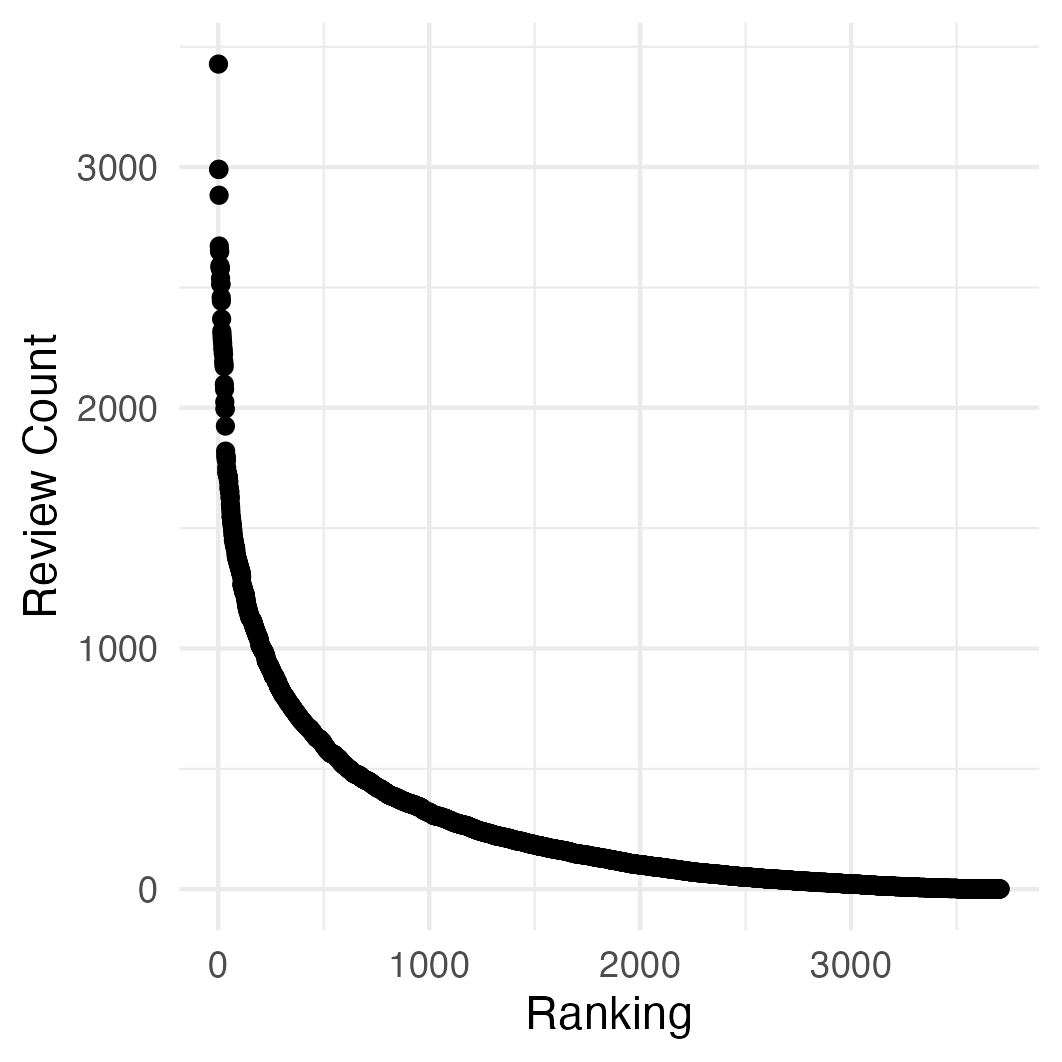
\includegraphics[width=\textwidth]{03_review_profile}
    \caption{Review profile.\label{fig:fig03_review_profile}}
  \end{subfigure}
  \begin{subfigure}{0.45\textwidth}
    \centering
    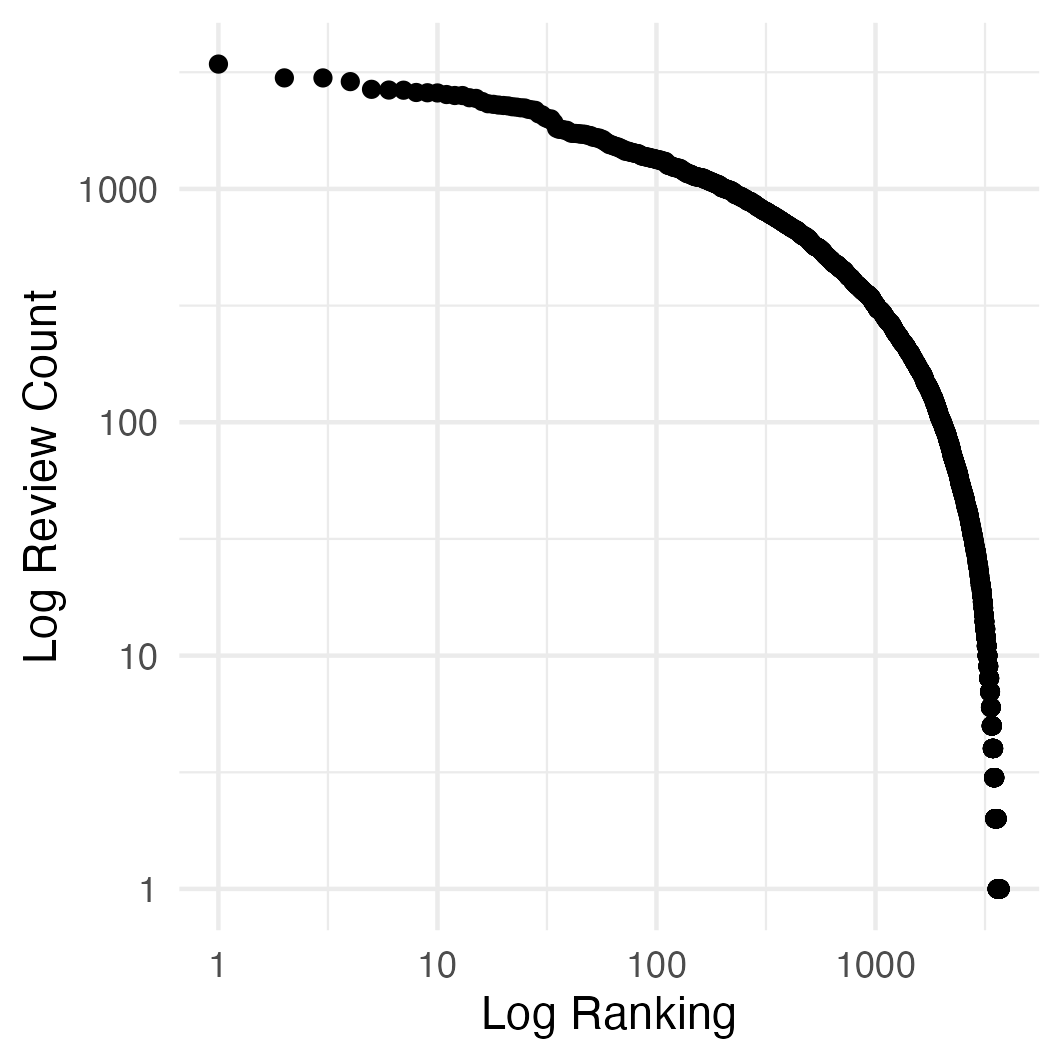
\includegraphics[width=\textwidth]{03_log_review_profile}
    \caption{Log-log plot.\label{fig:fig03_log_review_profile}}
  \end{subfigure}
  \caption{Review profile for the full dataset (a) and log-log
  plot (b).\label{fig:fig03_review_profile_both}}
\end{figure}

\subsection{Trivial Model}
\label{subsec:trivial}

Its recommendation profile can be seen in Figure~\ref{fig:fig1} and, since it is
the sum of many uniform samples, the number of times each movie is recommended
approaches a normal distribution and, therefore, the recommendation profile also
approaches the cumulative distribution function (CDF) of said distribution. The
most recommended movie appeared 25 times in the final list, while the least
recommended movie did not appear at all. Figure~\ref{fig:fig1b} shows the
log-log plot of the recommendation profile.

\begin{figure}
  \centering
  \begin{subfigure}{0.45\textwidth}
    \centering
    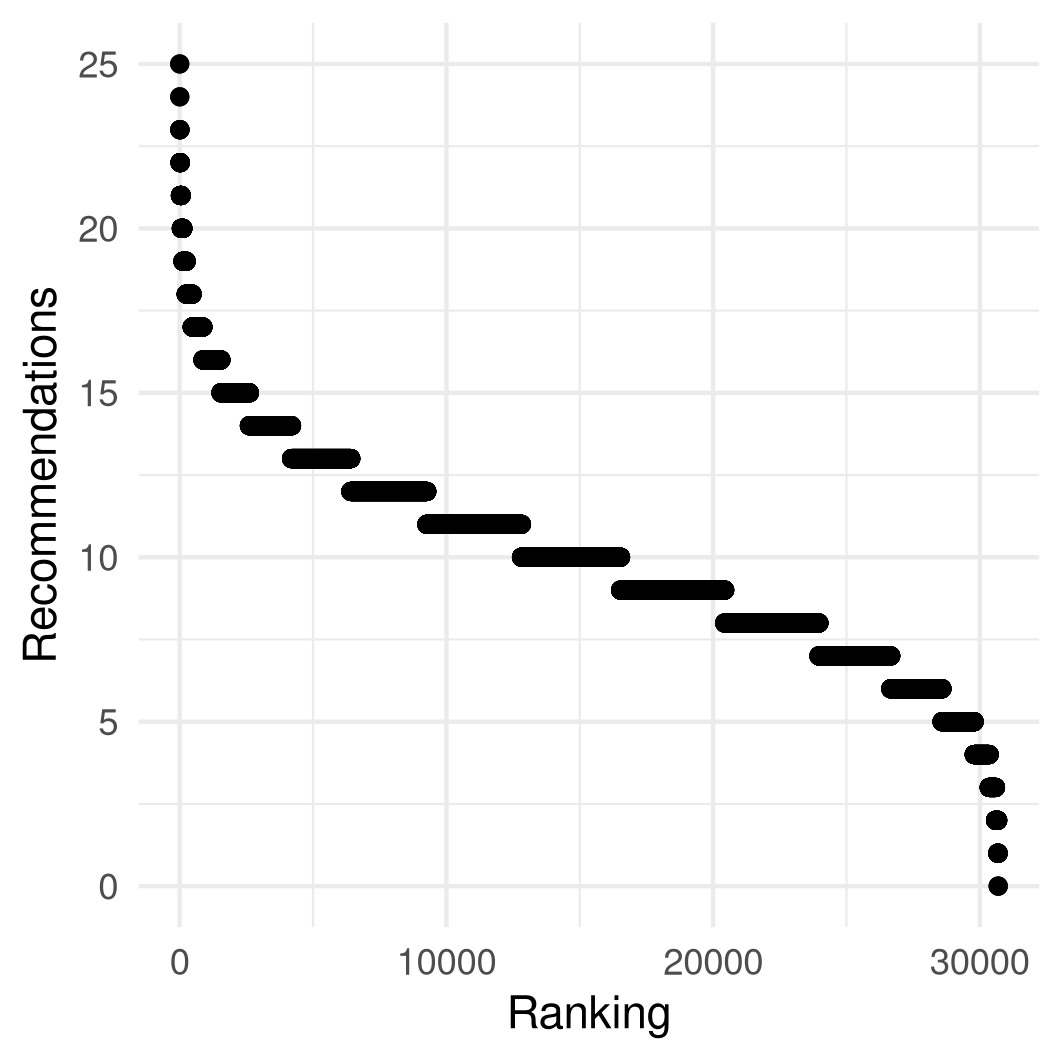
\includegraphics[width=\textwidth]{1a_random}
    \caption{Recommendation profile.\label{fig:fig1a}}
  \end{subfigure}
  \begin{subfigure}{0.45\textwidth}
    \centering
    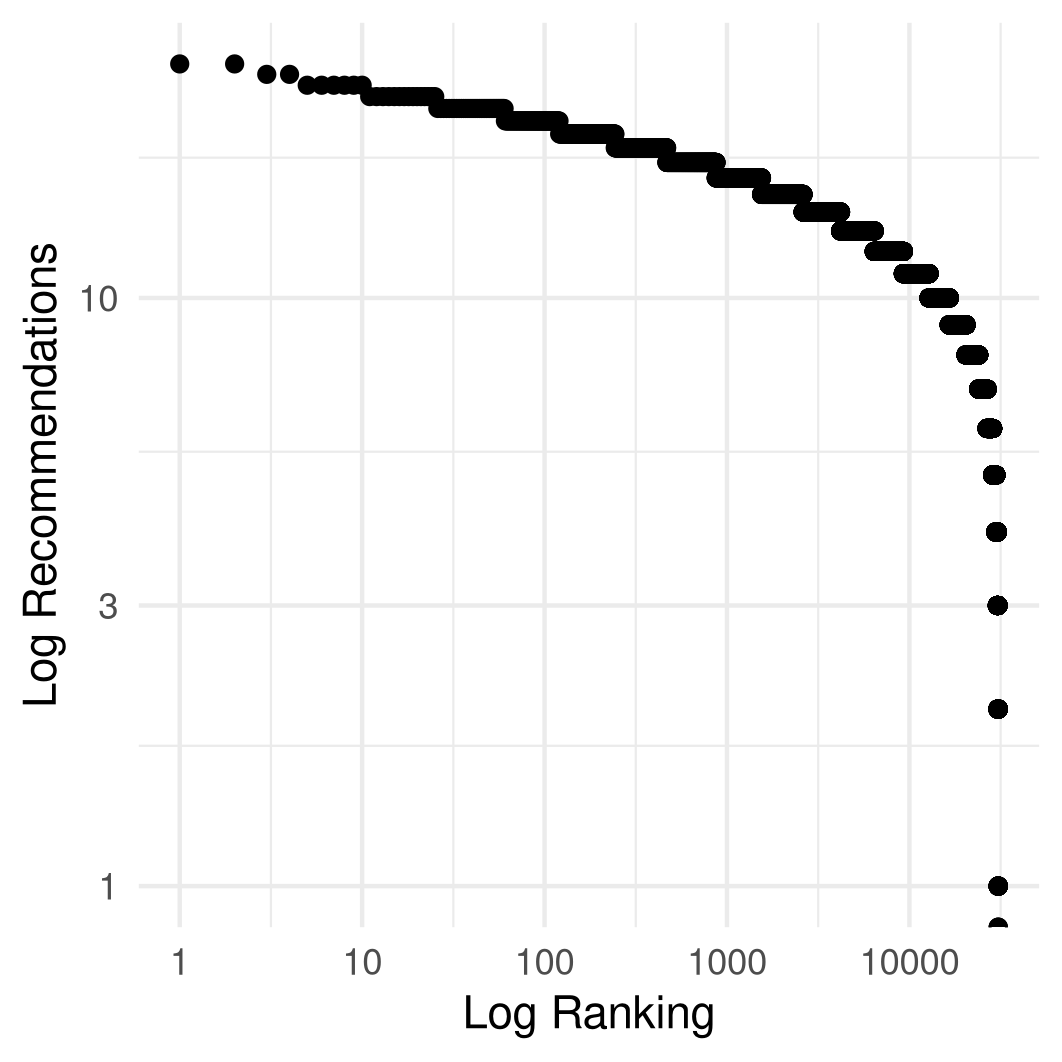
\includegraphics[width=\textwidth]{1b_random_log}
    \caption{Log-log plot.\label{fig:fig1b}}
  \end{subfigure}
  \caption{Recommendation profile for the trivial model (a) and log-log plot
    (b).\label{fig:fig1}}
\end{figure}

\subsection{Vanilla Model}
\label{subsec:vanilla}

The recommendation profile for the vanilla model can be seen in
Figure~\ref{fig:fig2a}. Here, the movie ranked number 1 appeared more than 2000
times in the full list of recommendations, with a power law decay in the number
of appearances from then on, as made evident by the log-log plot on
Figure~\ref{fig:fig2b}. This recommendation profile is a big departure from the
trivial model discussed above.

\begin{figure}
  \centering
  \begin{subfigure}{0.45\textwidth}
    \centering
    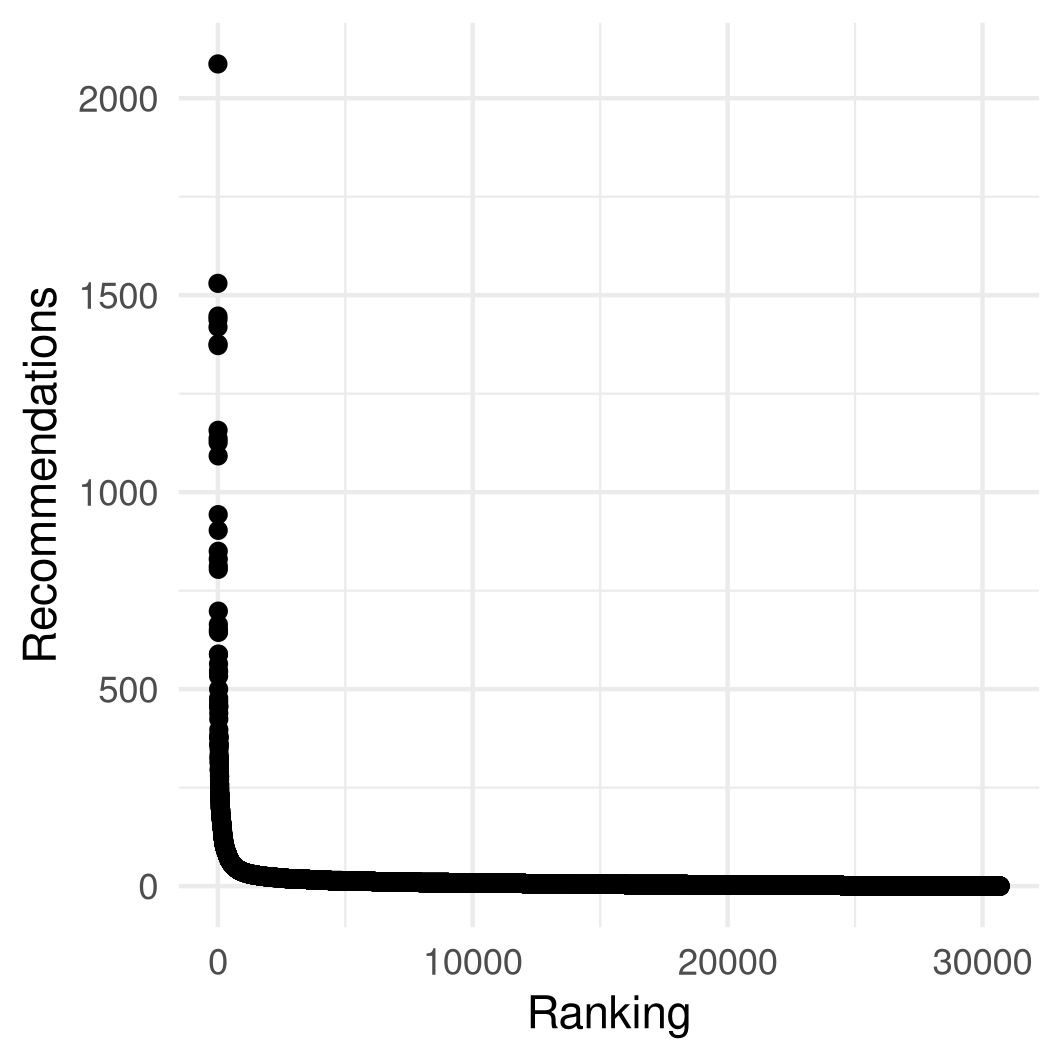
\includegraphics[width=\textwidth]{2a_vanilla}
    \caption{Recommendation profile.\label{fig:fig2a}}
  \end{subfigure}
  \begin{subfigure}{0.45\textwidth}
    \centering
    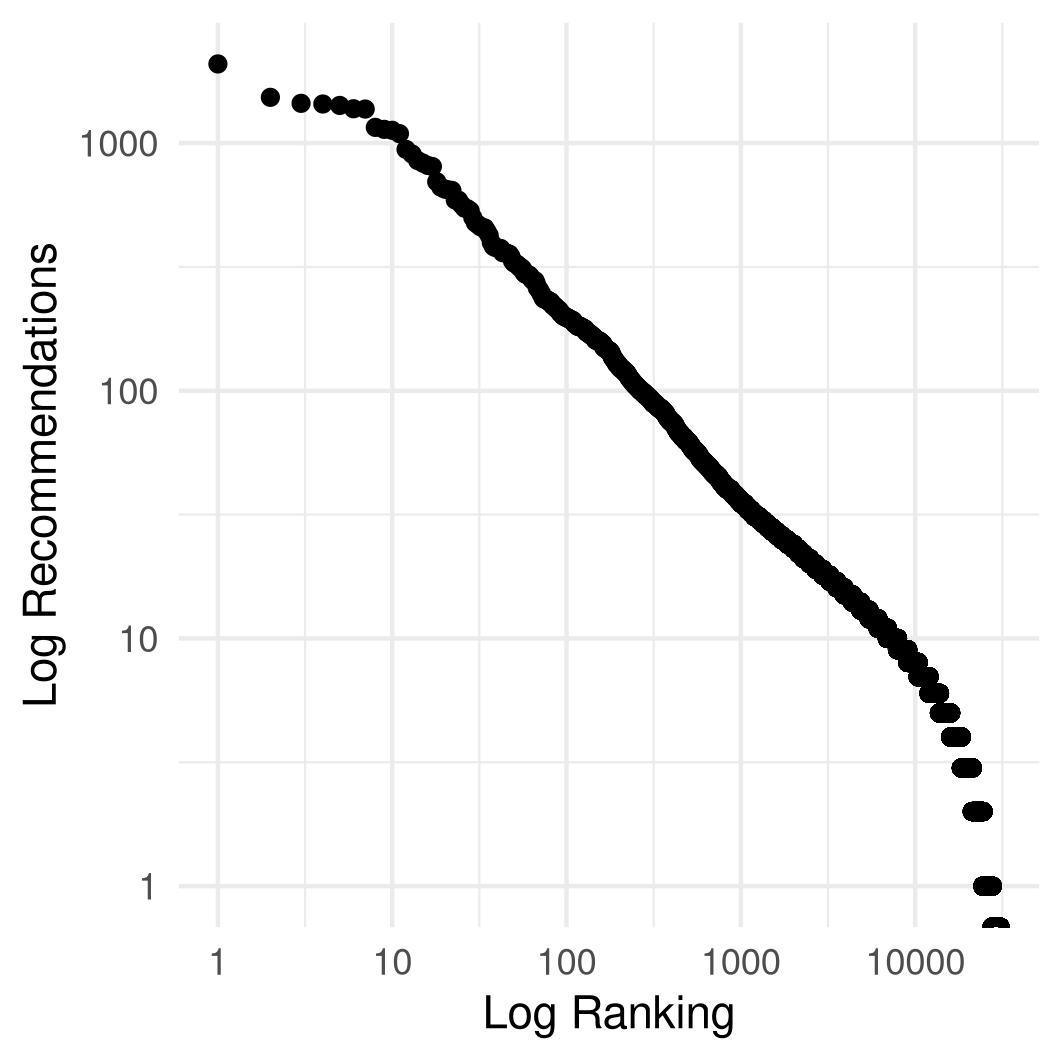
\includegraphics[width=\textwidth]{2b_vanilla_log}
    \caption{Log-log plot.\label{fig:fig2b}}
  \end{subfigure}
  \caption{Recommendation profile for the vanilla model (a) and log-log plot
    (b).\label{fig:fig2}}
\end{figure}

\subsection{Cutoff Models}
\label{subsec:cutoff}

A potential explanation for the difference between trivial and vanilla could
reside in the least used terms in the metadata and that is why we developed the
cutoff model. The results can be seen in Figure~\ref{fig:fig3} and, aside from
variations in the $y$-intercept, all plots are qualitatively very similar to
Figure~\ref{fig:fig2a}, indicating that rare words probably are not to blame for
the power law decay.

\begin{figure}
  \centering
  \begin{subfigure}{0.3\textwidth}
    \centering
    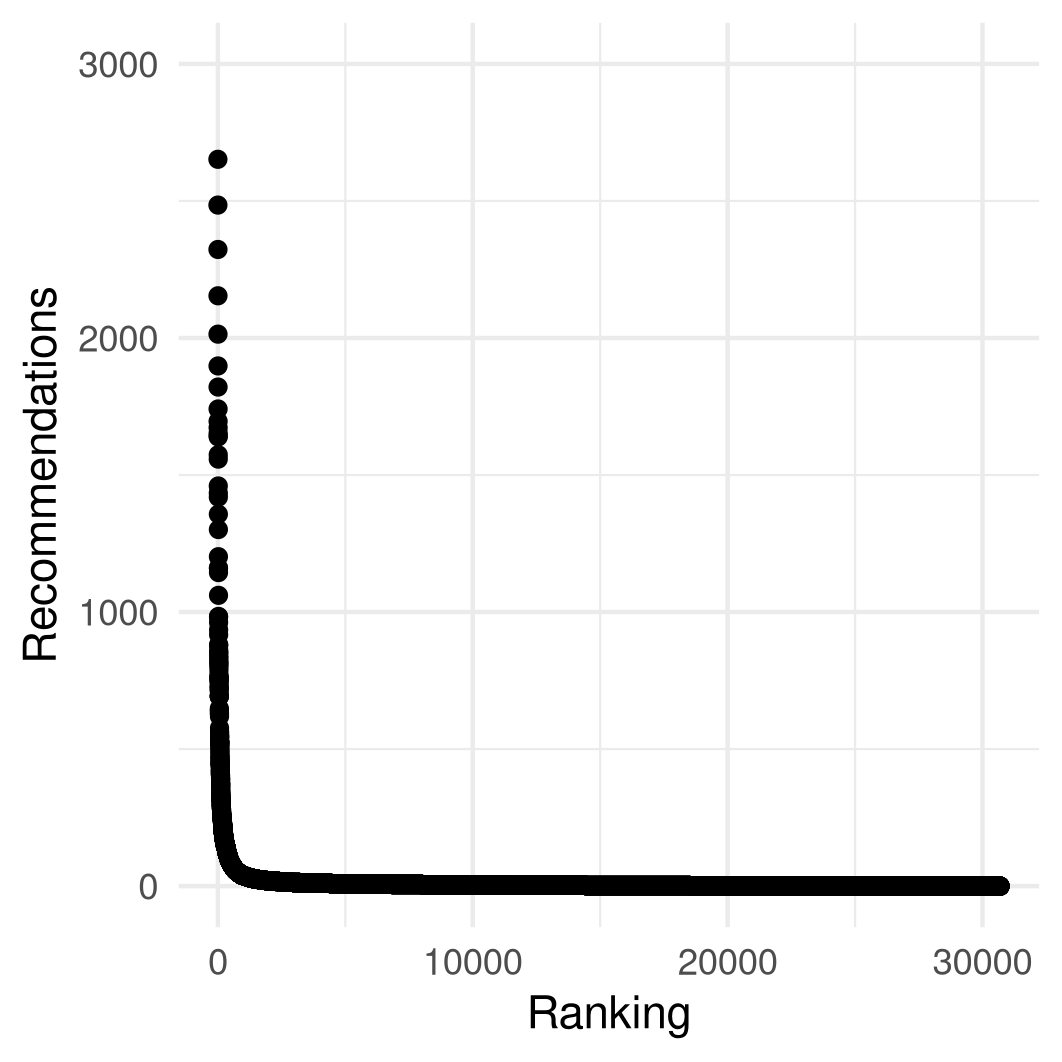
\includegraphics[width=\textwidth]{3a_cutoff_low}
    \caption{Cutoff $k = 2$.\label{fig:fig3a}}
  \end{subfigure}
  \begin{subfigure}{0.3\textwidth}
    \centering
    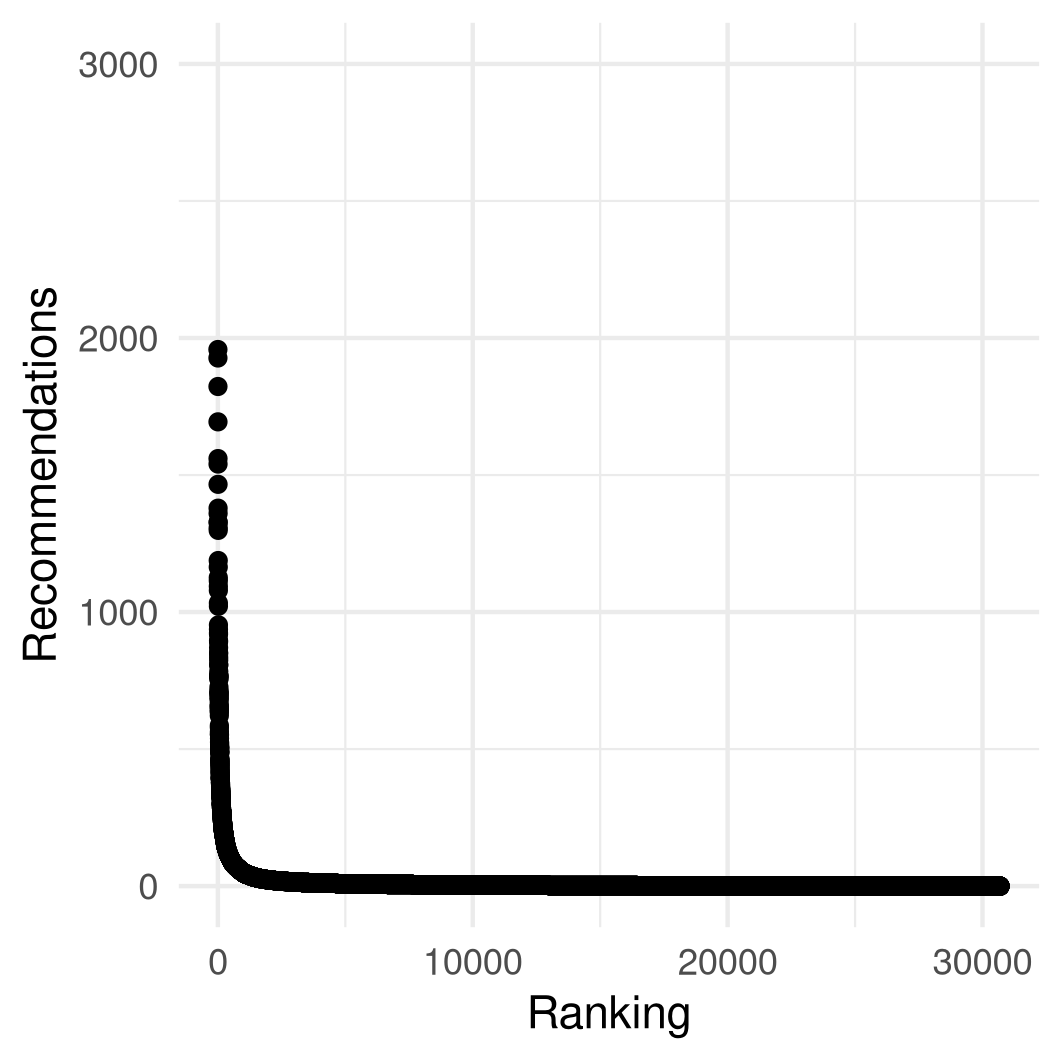
\includegraphics[width=\textwidth]{3b_cutoff_med}
    \caption{Cutoff $k = 5$.\label{fig:fig3b}}
  \end{subfigure}
  \begin{subfigure}{0.3\textwidth}
    \centering
    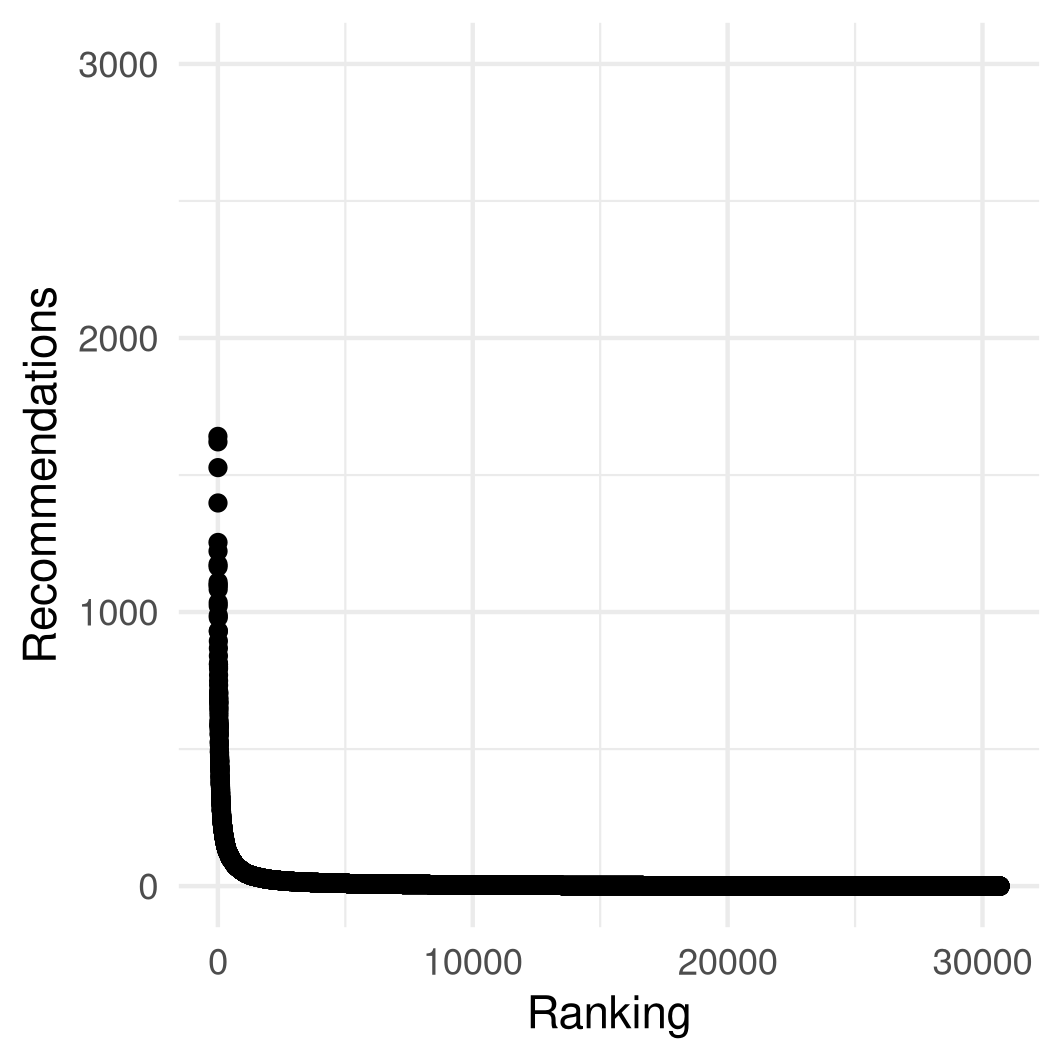
\includegraphics[width=\textwidth]{3c_cutoff_high}
    \caption{Cutoff $k = 8$.\label{fig:fig3c}}
  \end{subfigure}
  \caption{Recommendation profile for cutoff $k = 2$ (a), $5$ (b), and $8$
    (c).\label{fig:fig3}}
\end{figure}

\subsection{Similarity Models}
\label{subsec:similarity}

Since the similarity metric could also be a source of the strange behavior of
the recommendation profile, we conceived the three similarity models described
in the last section. Figure~\ref{fig:fig4} showcases a comparison between cosine
distance, euclidean distance and manhattan distance. It is clear that there are
no meaningful differences between the recommendation profiles generated by each
metric.

\begin{figure}
  \centering
  \begin{subfigure}{0.3\textwidth}
    \centering
    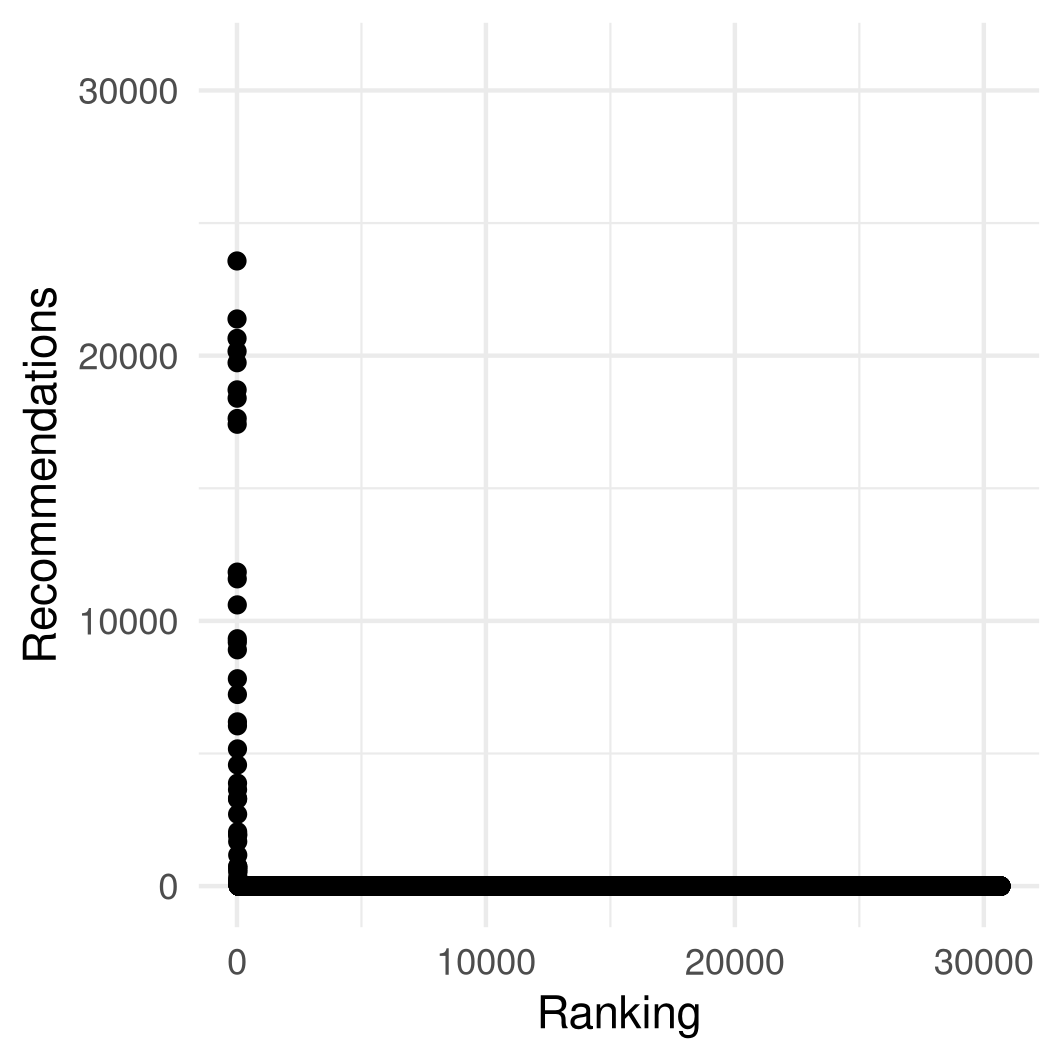
\includegraphics[width=\textwidth]{4a_cosine}
    \caption{Cosine distance (vanilla).\label{fig:fig4a}}
  \end{subfigure}
  \begin{subfigure}{0.3\textwidth}
    \centering
    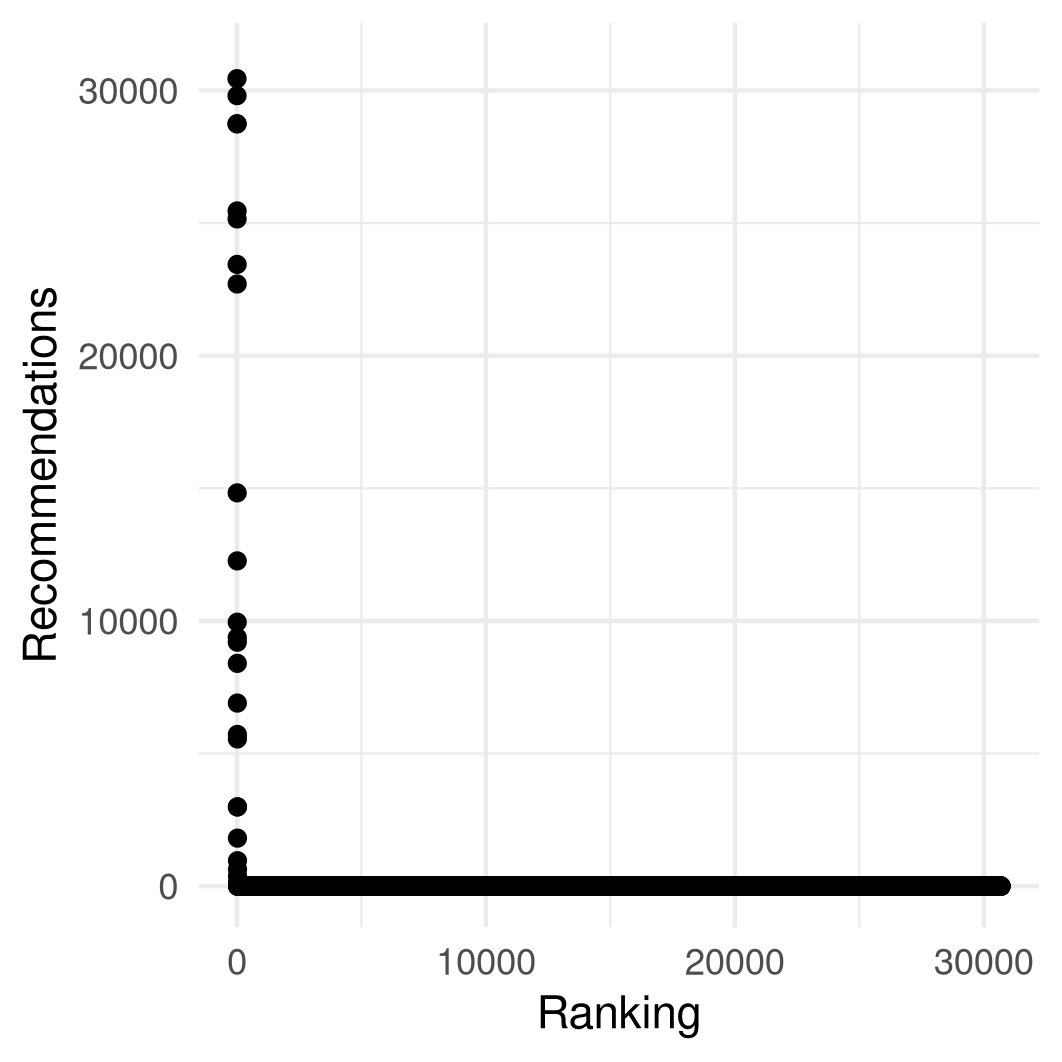
\includegraphics[width=\textwidth]{4b_euclidean}
    \caption{Euclidean distance.\label{fig:fig4b}}
  \end{subfigure}
  \begin{subfigure}{0.3\textwidth}
    \centering
    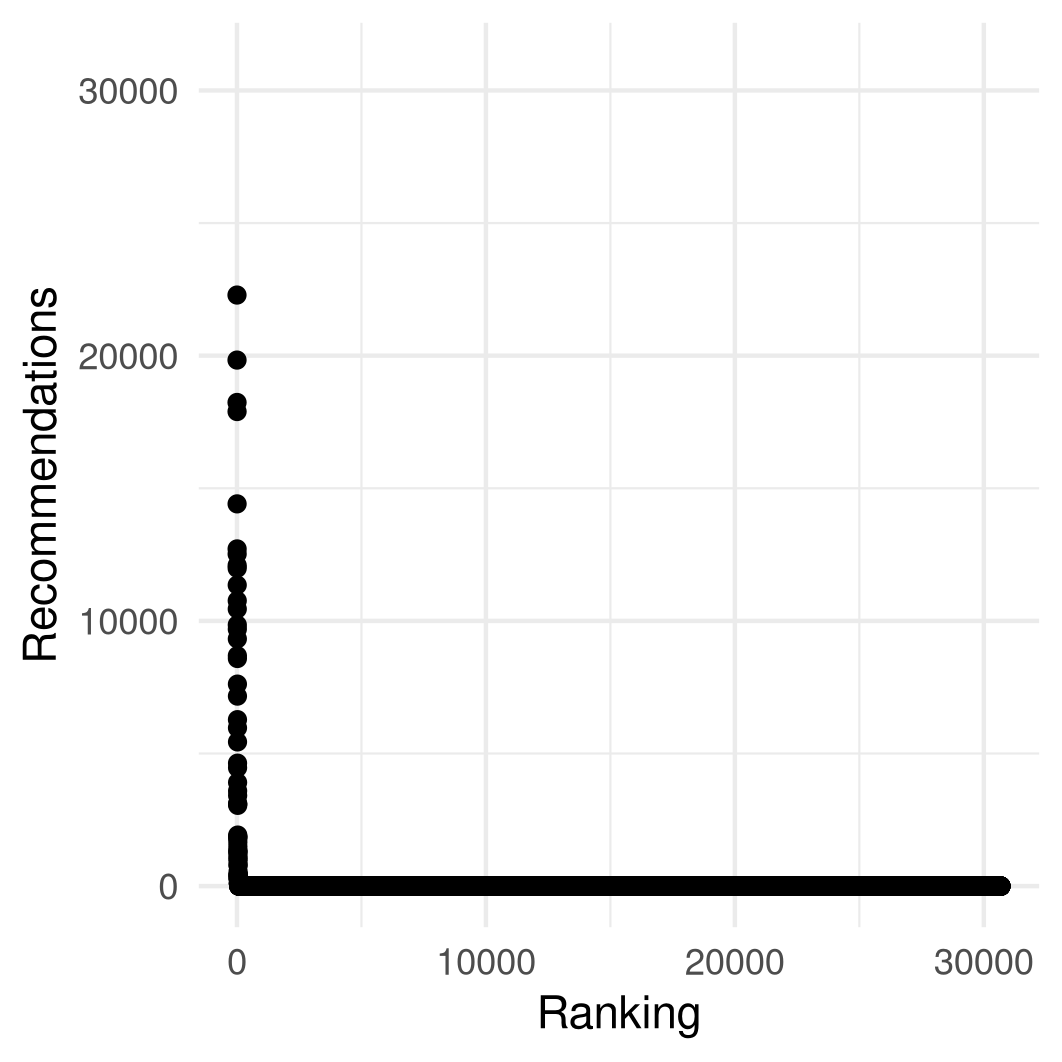
\includegraphics[width=\textwidth]{4c_manhattan}
    \caption{Manhattan distance.\label{fig:fig4c}}
  \end{subfigure}
  \caption{Recommendation profile for cosine (a), euclidean (b), and manhattan
    (c) distances.\label{fig:fig4}}
\end{figure}

\subsection{Vanilla Model with Synthetic Metadata}
\label{subsec:synthetic}

At this point it is safe to say that the type of decay seen in recommendation
frequencies up until now is not spurious and must have a clear cause. To better
investigate whether word frequency had an impact on the recommendation profiles
another hypothesis was taken into consideration: do metadata with less words
cause the recommendation curves to display a steep left-hand side?

Figure~\ref{fig:fig5} displays the recommendation profiles for the vanilla model
applied to datasets with synthetic metadata. Concretely, the figures are
equivalent to creating random metadata for the movies where the probability of
any single word being selected was approximately $1.54 \times 10^{-4}$, $1.54
\times 10^{-3}$, and $1.54 \times 10^{-2}$ respectively. The results do support
the aforementioned hypothesis since denser vectors indeed affected the decay.

\begin{figure}
  \centering
  \begin{subfigure}{0.3\textwidth}
    \centering
    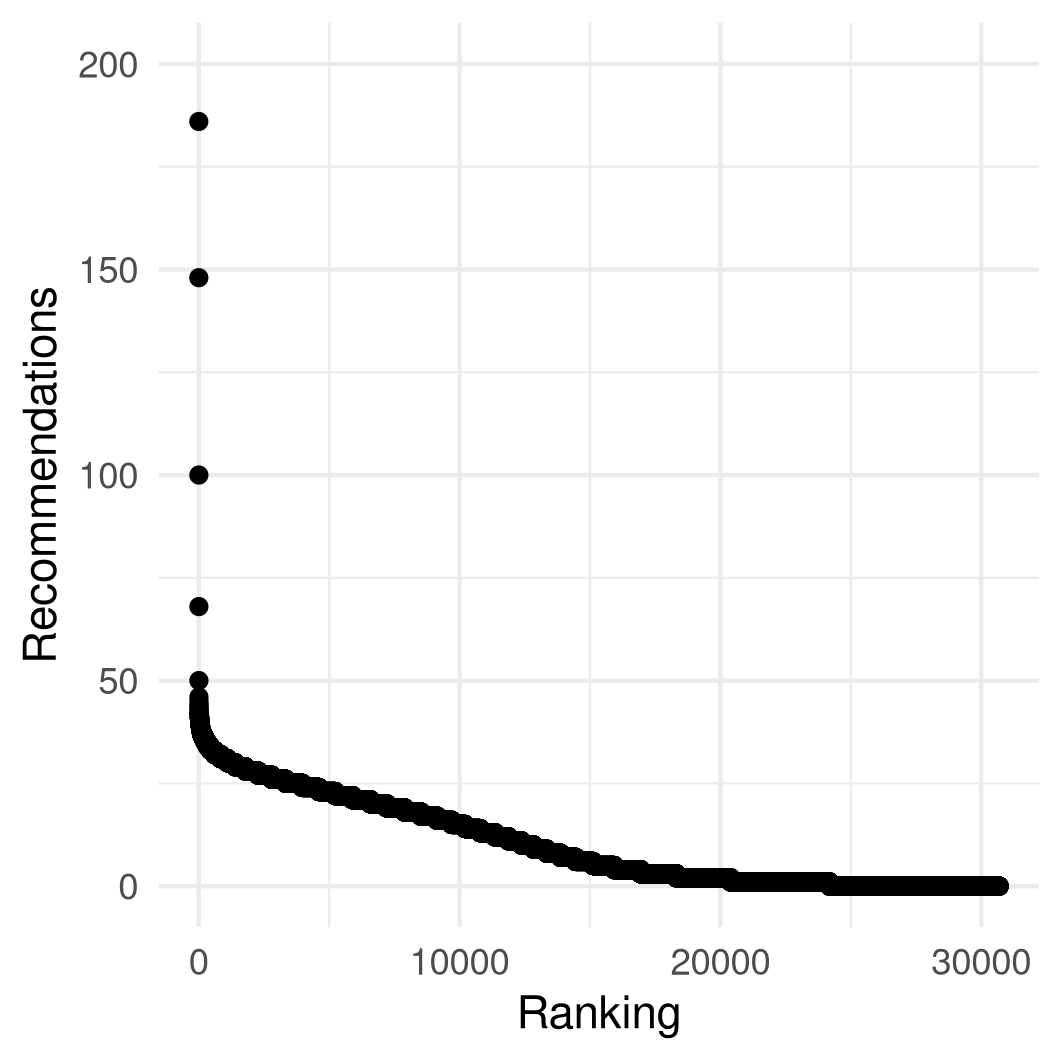
\includegraphics[width=\textwidth]{5a_p}
    \caption{$P(w_{i}) = 1 \times \overline{P(w)}$.\label{fig:fig5a}}
  \end{subfigure}
  \begin{subfigure}{0.3\textwidth}
    \centering
    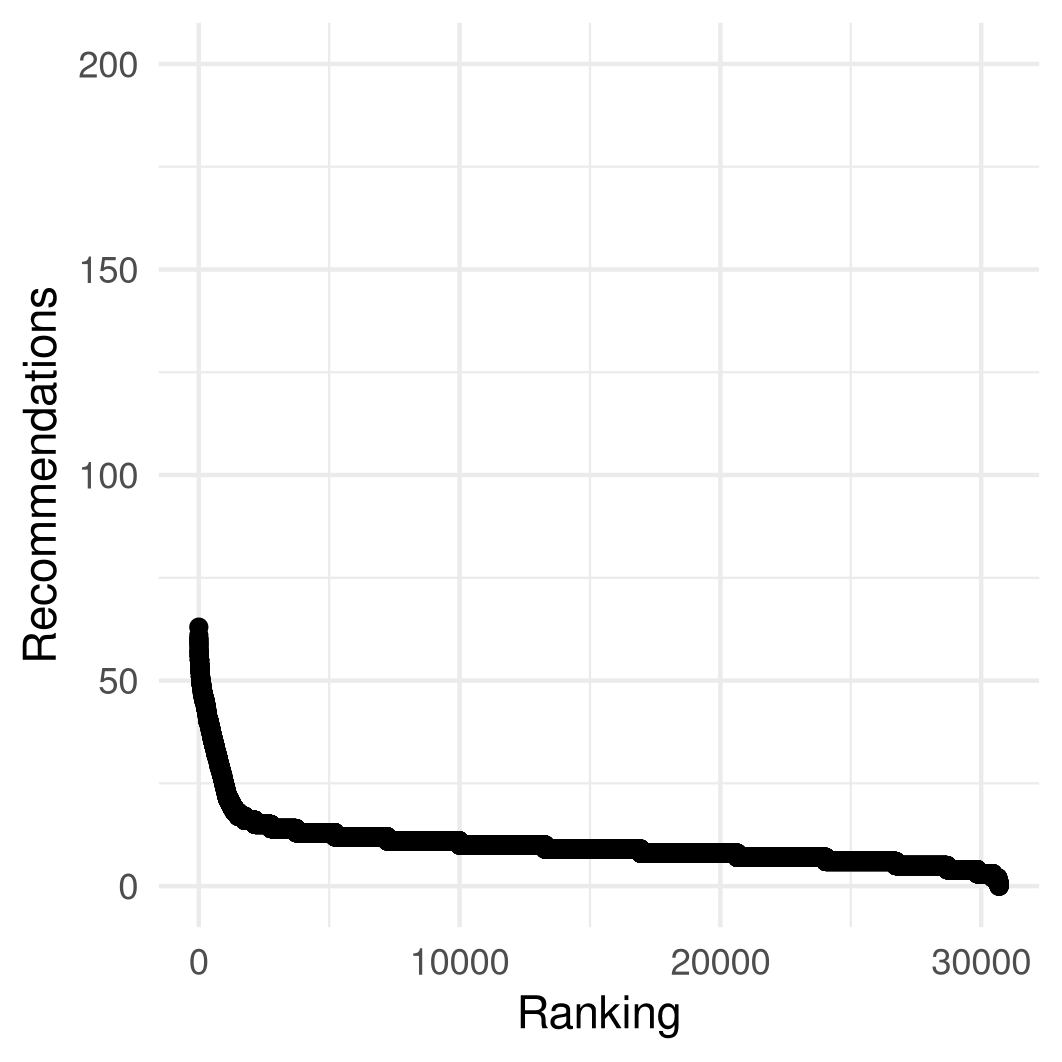
\includegraphics[width=\textwidth]{5b_p10}
    \caption{$P(w_{i}) = 10 \times \overline{P(w)}$.\label{fig:fig5b}}
  \end{subfigure}
  \begin{subfigure}{0.3\textwidth}
    \centering
    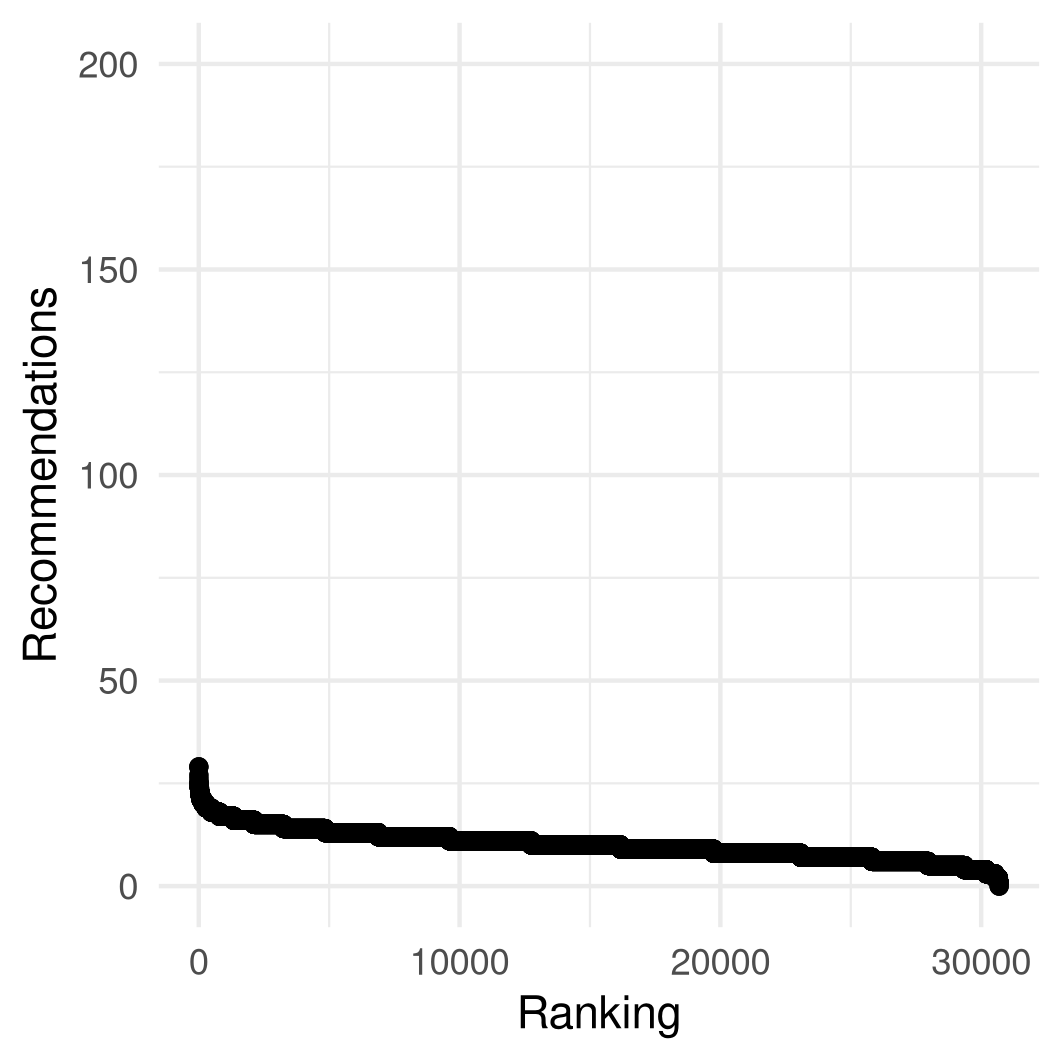
\includegraphics[width=\textwidth]{5c_p100}
    \caption{$P(w_{i}) = 100 \times \overline{P(w)}$.\label{fig:fig5c}}
  \end{subfigure}
  \caption{Recommendation profile of samples with
    $P(w_{i}) = C \times \overline{P(w)}$, $C = 1$ (a), $10$ (b), and $100$
    (c).\label{fig:fig5}}
\end{figure}

\subsection{Sanity Checks}
\label{subsec:sanity03}

After the previous experiments, sanity checks were needed in order to verify
that our previous results weren't spurious. The first check should check whether
an artificial movie created as a combination of the metadata from other movies
favored by the recommendation algorithm would also be favored (i.e. we are able
to create a popular movie from other popular movies), while the second should
check whether shorter vectors would change the decay already observed despite
being as sparse as their longer counterparts (i.e. the intrinsic properties of
the dataset aren't responsible for the power law decay). We repeated these tests
thousands of times and the results presented below are typical of what we found.

Figure~\ref{fig:fig6} showcases the two sanity checks. Figure~\ref{fig:fig6a}
was a model applied to the vanilla dataset with the addition of the movie
highlighted in red. As expected, this movie also showed up in the
top-recommended subset. Figure~\ref{fig:fig6b} comes from a model applied to
randomly generated vector representations in a similar fashion to the ones in
Figure~\ref{fig:fig5}, except each vector could only have 15,000 elements
instead of 55,681 (as with the vanilla model).

\begin{figure}
  \centering
  \begin{subfigure}{0.45\textwidth}
    \centering
    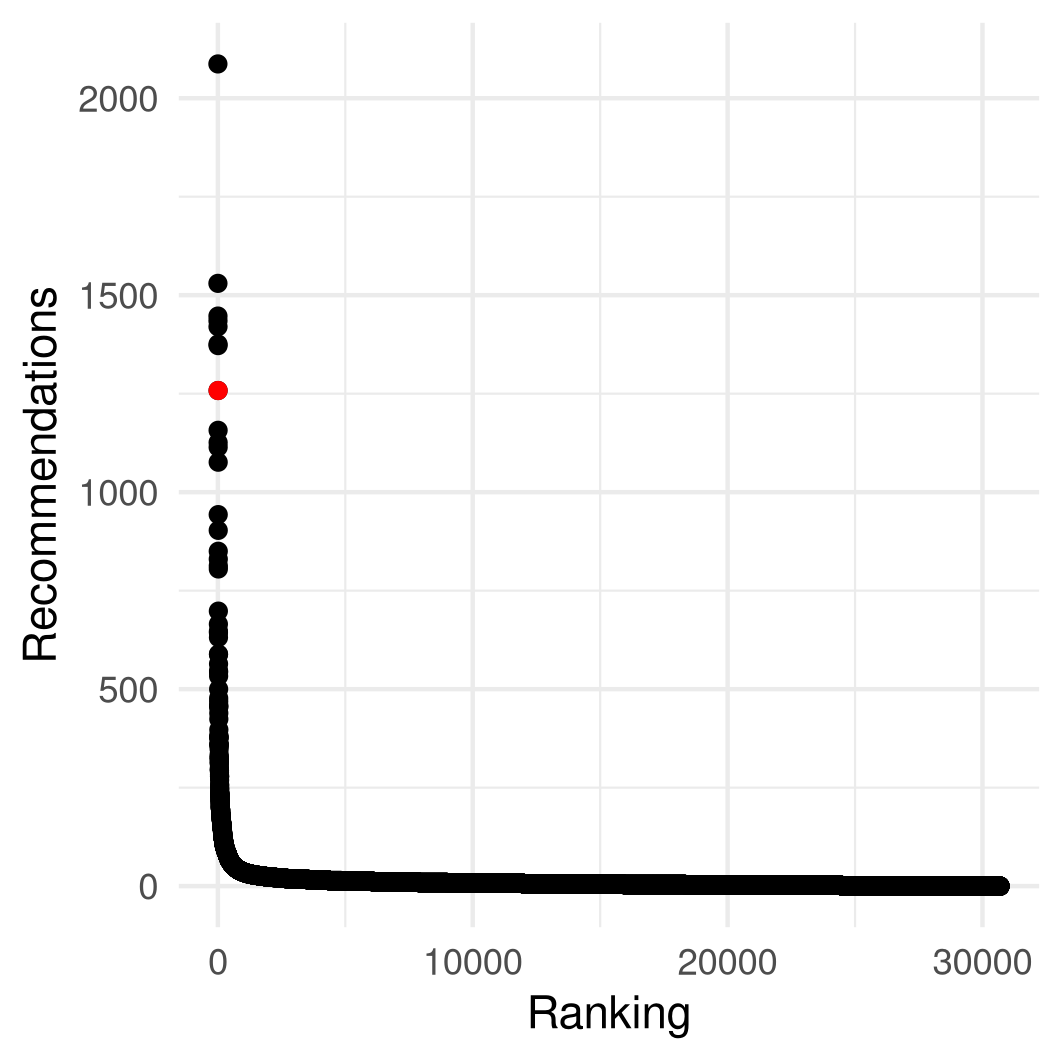
\includegraphics[width=\textwidth]{6a_artificial_movie}
    \caption{Vanilla model with artificial movie in red.\label{fig:fig6a}}
  \end{subfigure}
  \begin{subfigure}{0.45\textwidth}
    \centering
    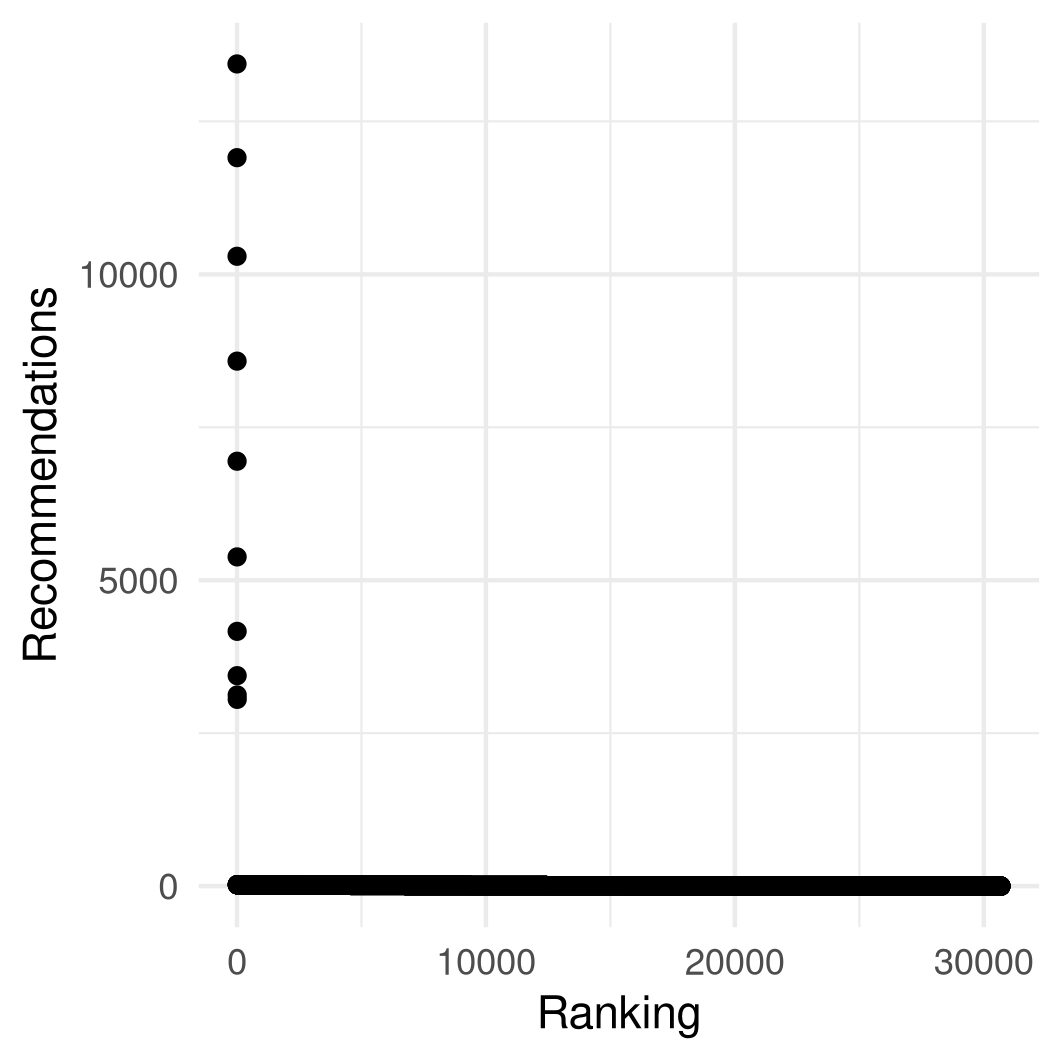
\includegraphics[width=\textwidth]{6b_long}
    \caption{Model with short vector representations.\label{fig:fig6b}}
  \end{subfigure}
  \caption{Recommendation profile for artificial movie (a) and short vector
    representations (b).\label{fig:fig6}}
\end{figure}

The last two models were considered the confirmations of the hypothesis that (at
least for this kind of recommendation systems) a subset of items was always much
more recommended than the rest as long as the data was sparse.
Figure~\ref{fig:fig7a} represents the same recommendation algorithm applied to
another dataset, the Book-Crossing dataset. Figure~\ref{fig:fig7b} contains the
results of the model applied to another set of random vector representations,
this time with the probability of each element being non-zero respecting the
marginal distributions of the vanilla dataset. Again, the power law decay
pattern persisted, only slightly less pronounced in the Book-Crossing case.

\begin{figure}
  \centering
  \begin{subfigure}{0.45\textwidth}
    \centering
    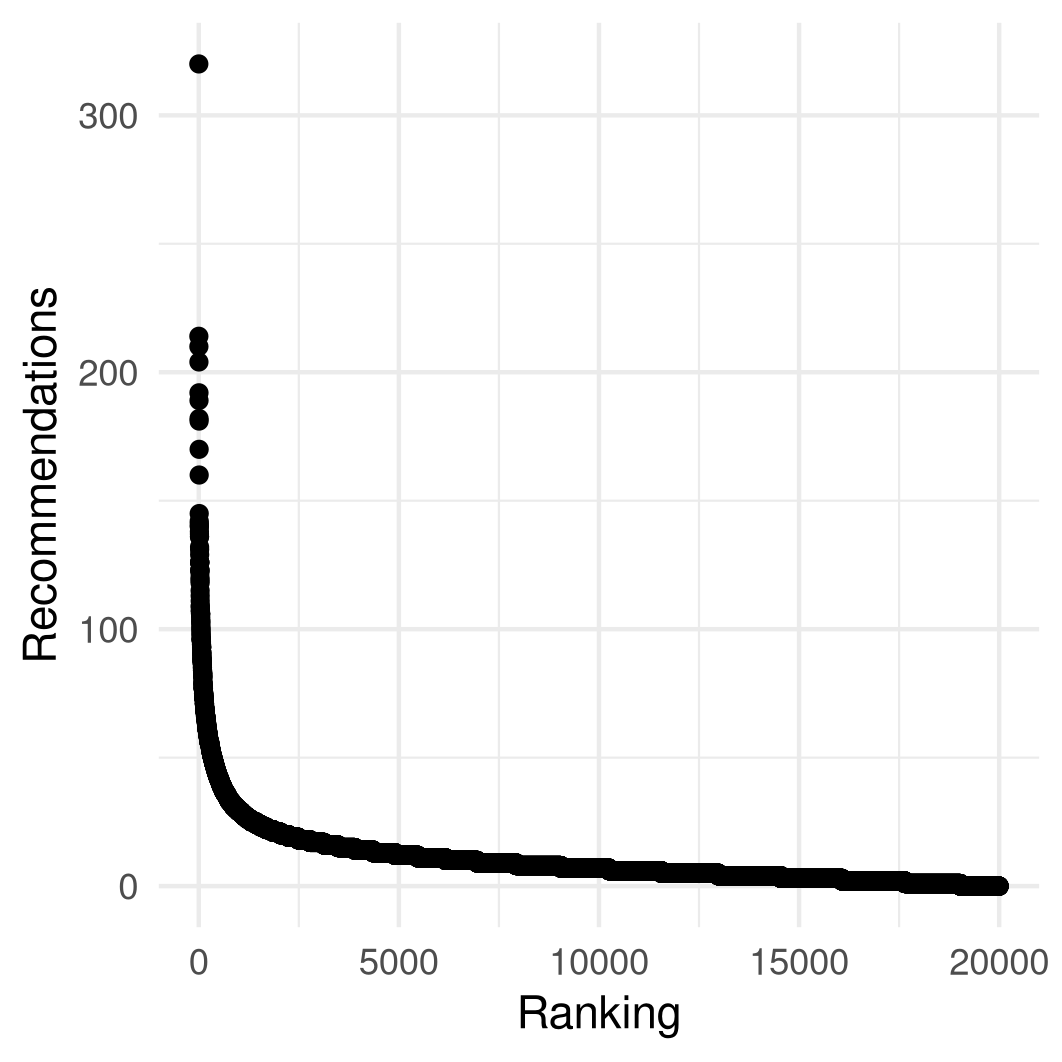
\includegraphics[width=\textwidth]{7a_books}
    \caption{Recommendation profile for book dataset.\label{fig:fig7a}}
  \end{subfigure}
  \begin{subfigure}{0.45\textwidth}
    \centering
    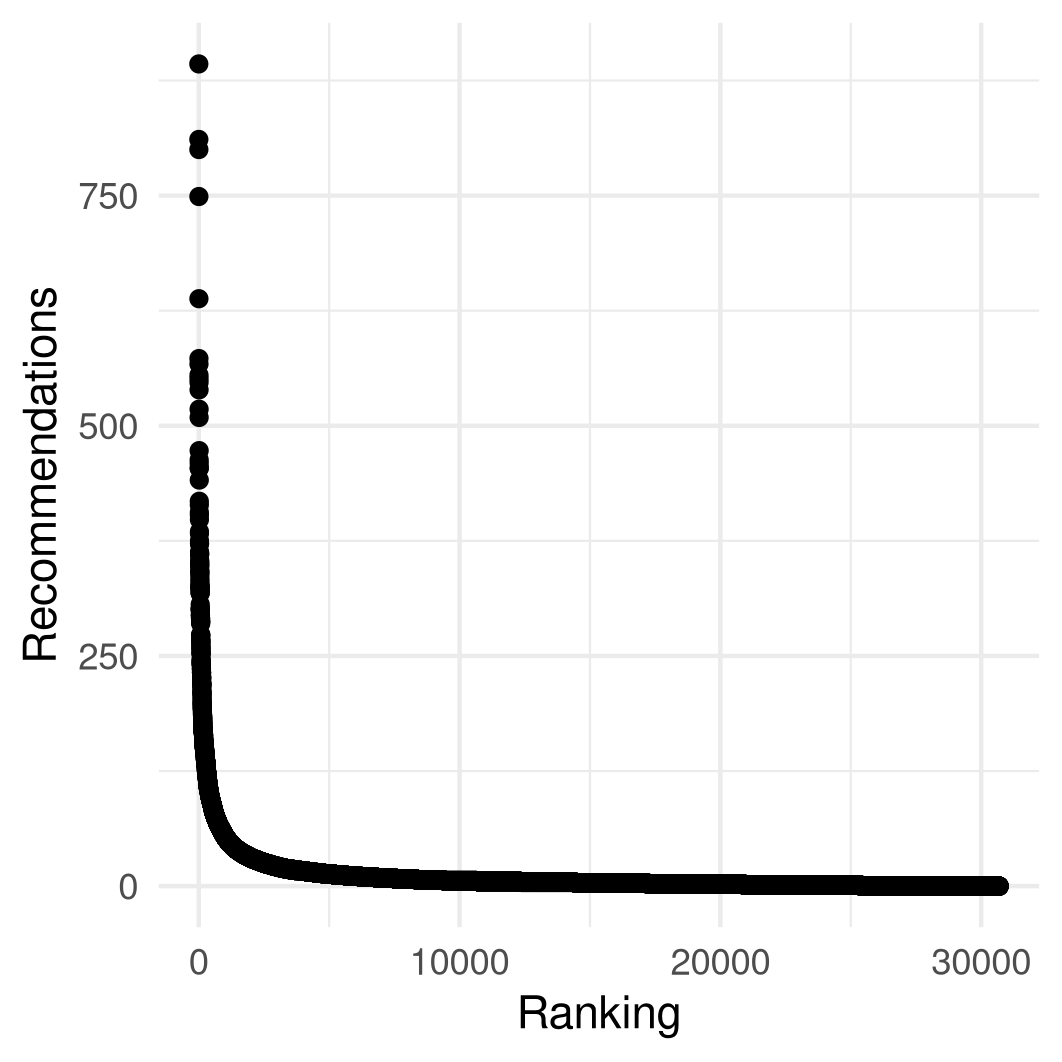
\includegraphics[width=\textwidth]{7b_mimic}
    \caption{Random simularion of vanilla.\label{fig:fig7b}}
  \end{subfigure}
  \caption{Recommendation profile for book dataset (a) and random simulation of
    vanilla (b).\label{fig:fig7}}
\end{figure}

The analysis up until now has been static, that is, the recommendation model
does not learn from the users' responses to its suggestions. There is no
interaction with users and no opportunity to evolve over time. The next chapter
addresses this point by using Google's newly released TensorFlow Recommenders
library \citep{noauthor_tensorflow_nodate} to gather data about what happens to
a system's recommendations as users follow its suggestions. Employing a deep
learning model that is able to improve over time is a significant departure from
the content-based models presented here and, if a similar recommendation profile
can also be detected for multi-criteria recommender systems on dynamic
scenarios, then the hypothesis ventilated in the section above would become even
more plausible.

\par

%!TeX root=../tese.tex
%("dica" para o editor de texto: este arquivo é parte de um documento maior)
% para saber mais: https://tex.stackexchange.com/q/78101/183146

\chapter{Dynamic Analysis}
\label{cap:dynamic}

Following the static analysis, it became clear that a dynamic analysis would be
of the utmost importance. Understanding how the recommendation model responds to
users reinforcing its internal biases, like the ones already detected, could
potentially lead to a better understanding of how these systems favor certain
kinds of content.

In order for this analysis to be more true to reality, we implemented a simple
recommendation algorithm using TensorFlow Recommenders \citep{}, a library for
machine learning developed by Google for use with its TensorFlow \citep{}
framework. This means that, even though our model is deliberately bare-bones, it
conforms to industry-standard technology and practices.

The choice to use a simple recommendation algorithm instead of a more complex
one was twofold: first, we didn't want to use a model that could introduce many
confounding parameters to the analysis (e.g. hyperparameters, hardware
requirements, etc.), and second, we wanted to study a baseline that could, in
the future, be used as a comparison point for more complex algorithms.

The goal of this analysis is to gather data on how the recommendation system
behaves over time. As will be explained in the next sections, is to understand
what happens to the recommendation profile of the algorithm as it interacts with
itself via users that follow the generated suggestions.

The expectation is that the recommendation profile will grow ever more steep,
which is a reasonable guess; if the users reinforce the beliefs of the
algorithm, then is stands to reason that it will recommend popular movies with
more and more frequently, to more and more users. How much more frequently,
however, is the true question.

For the sake of clarity, let's imagine two users with very distinct preferences:
Alice, who enjoys adventure movies, and Bob, who enjoys horror movies. In
principle, the algorithm should have very different recommendations for both of
them and, were they to follow them, their custom suggestions should grow
increasingly different. At the end of this experiment, users like Alice would
all be recommended the same movies, and users like Bob would have their own set
of very popular films; we should expect, therefore, a multimodal distribution of
the recommendation frequencies, with "typical" adventure movies and "typical"
horror movies being much more popular than comedy, for example.

However, if the final recommendation profile looked like what was showcased in
the previous chapter, i.e. a very small subset of movies being recommended to
most users, then we could infer that the system devolved into a degenerate
feedback loop, ignoring personal preferences and distinctions between films.

\section{Datasets}
\label{sec:datasets04}

For the dynamic experiments, we kept using the Movielens dataset \citep{}. This
time, however, we used the full ``1M'' dataset instead of sampling movies from
the larger ``25M'' version. Given that we wanted our dynamic analysis to be
conducted in a realistic scenario, we decided that it would be better not to
change the data. This whole experiment will, therefore, use a version of the
dataset commonly used for machine learning benchmarks with no alteration
whatsoever.

The 1M dataset contains 1,000,209 ratings of almost 4000 movies made by over
6000 anonymous MovieLens users who joined the platform in 2000. In this
particular version, each user has made at least 20 ratings. There are 4 columns
available:

\begin{itemize}
  \item \verb|UserID|: Unique user identifier, ranging from 1 to 6040.
  \item \verb|MovieID|: Unique movie identifier, ranging from 1 to 3952.
  \item \verb|Rating|: Movie rating according to user, from 0 to 5 stars.
  \item \verb|Timestamp|: When the user made the rating, in seconds since the
  epoch.
\end{itemize}

A second, auxiliary, dataset was also used to enrich the main one. ``Movies''
contains extra information about the movies in 1M, which allowed us to add more
variables to the recommendation system. This new dataset has 3 columns:

\begin{itemize}
  \item \verb|MovieID|: Unique user identifier, ranging from 1 to 6040.
  \item \verb|Title|: Title of the movie, as provided by IMDB.
  \item \verb|Genres|: Pipe-separated string with all applicable genres.
\end{itemize}

The other accompanying dataset, ``Users'', has not been used for the purposes of
this analysis. The reasoning behind this decision will be explained in greater
detail in the next section.

\section{Experiments}
\label{sec:experiments04}

The dynamic experiment starts in a manner much similar to the static experiment.
The full MovieLens dataset is fed as training data to a recommendation system in
order to get it ready for giving suggestions to users. As explained in the
opening section of this chapter, we chose a simple algorithm in order to reduce
the number of possible interferences architecture could have on our analysis.

The chosen recommendation algorithm was a basic ranking model described in
\citet{} using TensorFlow Recommenders \citep{}. It is composed of multiple
stacked dense layers and uses mean squared error as its loss function. The main
class in the model is reproduced below, and the full algorithm is listed in
Appendix~\ref{}.

%% Deixar o código em pseudo-código para ficar mais claro

\begin{verbatim}
class MovielensModel(tfrs.models.Model):

  def __init__(self):
    super().__init__()
    self.ranking_model: tf.keras.Model = RankingModel()
    self.task: tf.keras.layers.Layer = tfrs.tasks.Ranking(
      loss = tf.keras.losses.MeanSquaredError(),
      metrics=[tf.keras.metrics.RootMeanSquaredError()]
    )

  def call(self, features: Dict[str, tf.Tensor]) -> tf.Tensor:
    return self.ranking_model(
        (features["user_id"], features["movie_title"]))

  def compute_loss(self, features: Dict[Text, tf.Tensor],
                    training=False) -> tf.Tensor:
    labels = features.pop("user_rating")

    rating_predictions = self(features)

    # The task computes the loss and the metrics.
    return self.task(labels=labels, predictions=rating_predictions)
\end{verbatim}

In the first step of the experiment, we trained the recommendation model using
Movielens' 1M ratings dataset, which we will refer to as \verb|ratings0| from
now on. All available data was used and, in the end, we achieved a root mean
squared error (RMSE) of 0.92; this result is similar to TFRS' deep \& cross
network \citep{} results when trained on the same data. Once \verb|model0| was
ready for making recommendations, we applied it to every possible user-movie
pairing, generating a complete matrix of predicted ratings called
\verb|predictions0|.

In an environment like YouTube's recommendations sidebar, the user is presented
with a few items that the algorithm thinks they would like, and then they can
either ignore the sidebar or select one of the options to watch. Since our goal
was to explore what would happen when the recommendation system entered a
feedback loop, we picked one movie at random from each user's 10 best-ranked
entries.

This set of well-ranked movies was our way of simulating thousands of users
simultaneously approving of the algorithms recommendations and selecting one
option from their sidebars. The last step involved removing the oldest rating of
each each user from \verb|ratings0| and appending these these selections to the
dataset in order to create \verb|ratings1|. The full data flow is illustrated
in Figure~\ref{fig:fig04_dynamic_diagram}

\begin{figure}
  \centering
  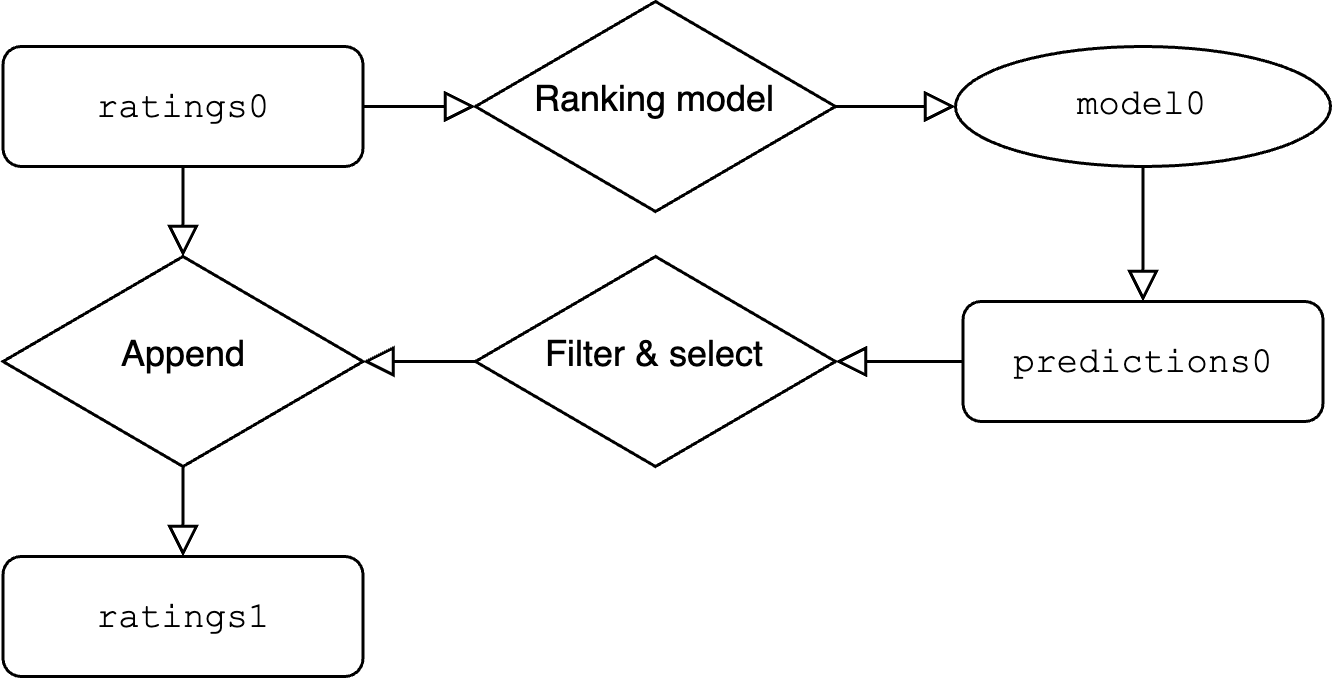
\includegraphics[width=\textwidth]{04_dynamic_diagram}
  \caption{Data flow diagram.\label{fig:fig04_dynamic_diagram}}
\end{figure}

% Explicar o que são os formatos no caption da figura.

A feedback loop, however, can't be created from a single iteration. For this
reason, the process just described was classified as the ``zeroth'' iteration in
the process (as it involved \verb|ratings0|). The ``first'' iteration began with
\verb|ratings1|, trained \verb|model1|, generated \verb|predictions1|, and ended
with \verb|ratings2|. We repeated this process until we got to \verb|ratings4|,
totaling 5 ratings datasets (one original and 4 derived through ranking models).

A simplified version of the R code that created \verb|ratingsN+1| from
\verb|ratingsN| can be found below. The omitted functions served mostly
auxiliary purposes which made the datasets conform to TensorFlow's format
expectations. The full code is listed in Appendix~\ref{}.

\begin{verbatim}
predictions |>
  group_by(user_id) |>
  slice_max(prediction, n = 10) |>
  slice_sample(n = 1) |>
  ungroup() |>
  bind_rows(old_ratings) |>
  group_by(user_id) |>
  slice_max(timestamp, n = -1, with_ties = FALSE) |>
  ungroup()
\end{verbatim}

With these new datasets we were able to analyze the differences between distinct
generations of models and understand exactly how the positive feedback loop
influenced the last iteration.

A series of analysis were conducted using these datasets as sources. We found
that, with each iteration, the recommendation profile got steeper and steeper,
that is, a few popular items got more recommended while the rest fell into
disfavor; this was predictably more noticeable in movies with higher average
ratings. In fact, a small set of around 20 movies were the only ones that
consistently rose in popularity with new iterations.

Figure~\ref{fig:fig04_profile_grouped} has five subplots which represent each
iteration of the recommendation system. For \verb|ratings0|, it's possible to
see that a number of well-rated movies were more popular, i.e., were rated by
more people. Once we generate the first batch of recommendations, we add up the
number of users each movie was recommended to; this is seen in the second plot,
\verb|ratings1|. We can clearly see that a small subset of movies strayed from
the pack and to more people that had watched them previously.

This process repeats itself until, in \verb|ratings4|, the most popular movie is
recommended more than 2000 times, while the most popular movie in
\verb|ratings0| was watched a little over 500 times.

As explained before, we expected that movies which where already popular would
be recommended more times, but these plots indicate a powerful feedback loop.
Examining the data, we saw that the algorithm was consistently recommending
movies which the users had already watched and this process only became more
accentuated with each subsequent iteration.

\begin{figure}
  \centering
  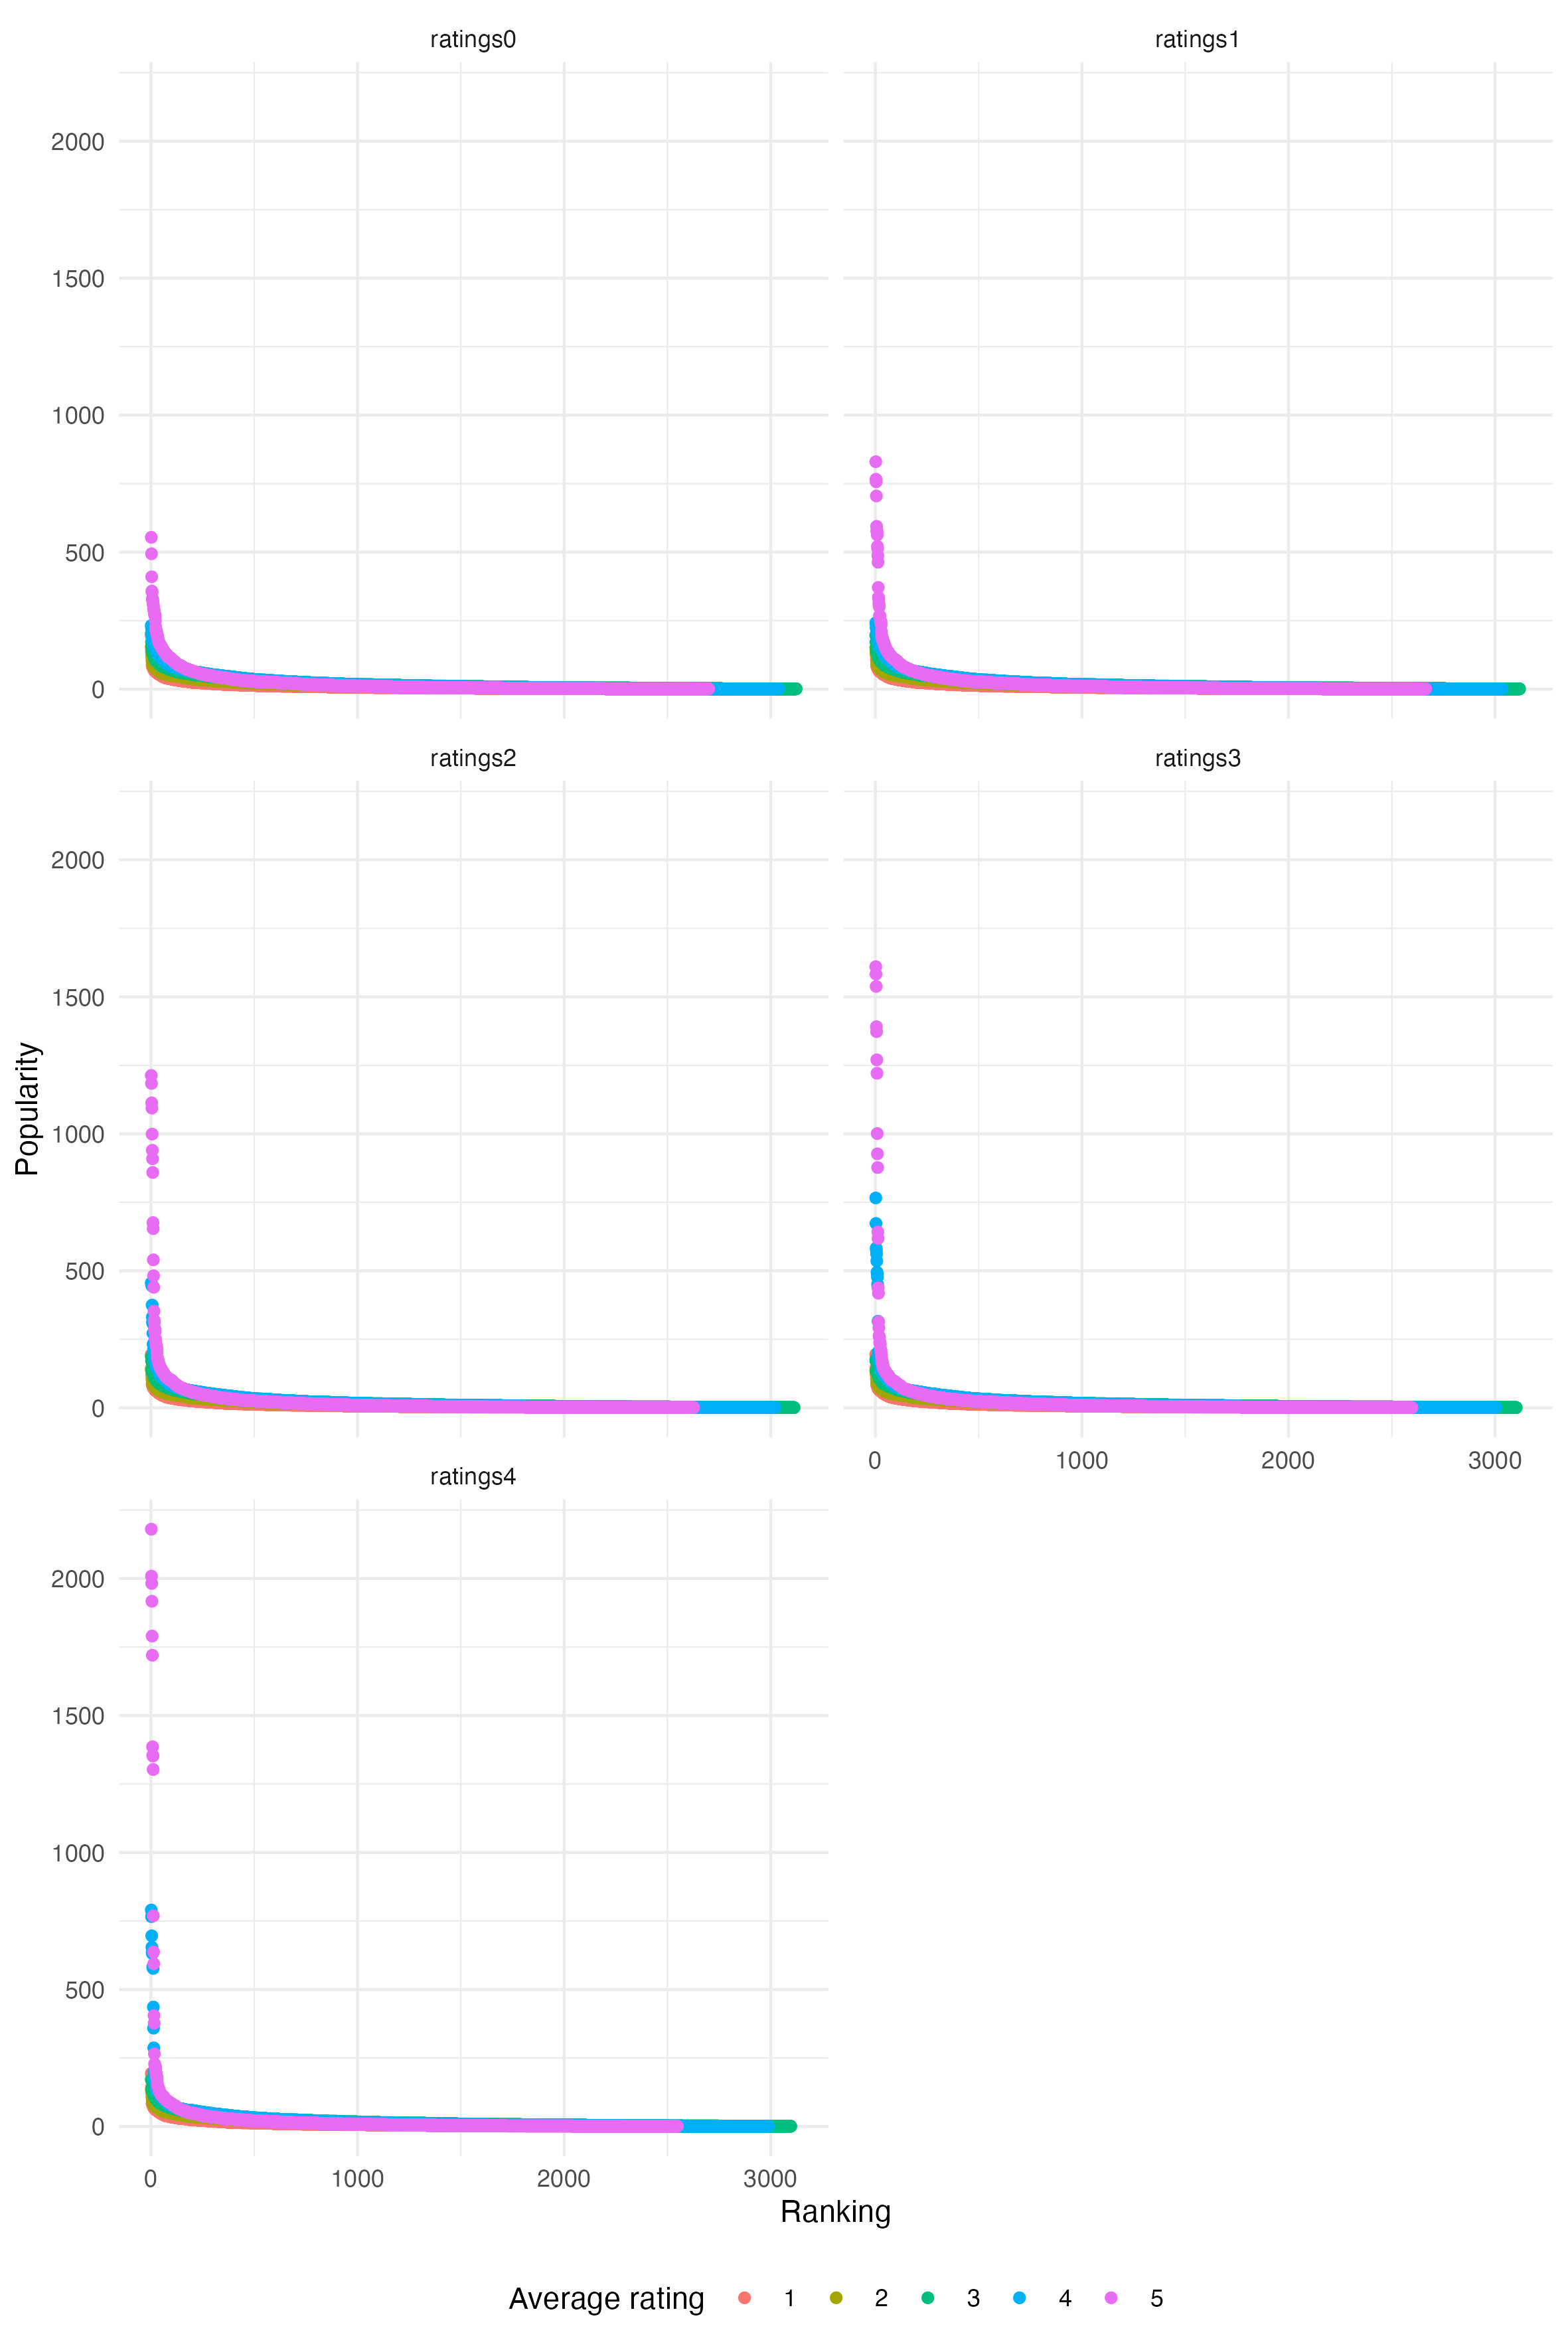
\includegraphics[width=\textwidth]{04_profile_grouped}
  \caption{Recommendation profile of every generation. Colors indicate average
  movie rating, which is a strong predictor of popularity over time.
  \label{fig:fig04_profile_grouped}}
\end{figure}

% explicar que, nos gráficos, popularidade significa número de recs para t = 1..4

A good way to measure how diverse were the recommendations made by the algorithm
is to calculate the entropy \citep{} of each set. In the extreme, if the same
movie is recommended to every user, than the entropy of the recommendations will
tend to zero. In absolute terms, the entropy of \verb|ratings0| was 7.42, and
the entropy of \verb|ratings4| was 6.08 (82\% lower). A comparison in relative
terms is displayed in Figure~\ref{fig:fig04_entropy}.

\begin{figure}
  \centering
  \begin{subfigure}{0.45\textwidth}
    \centering
    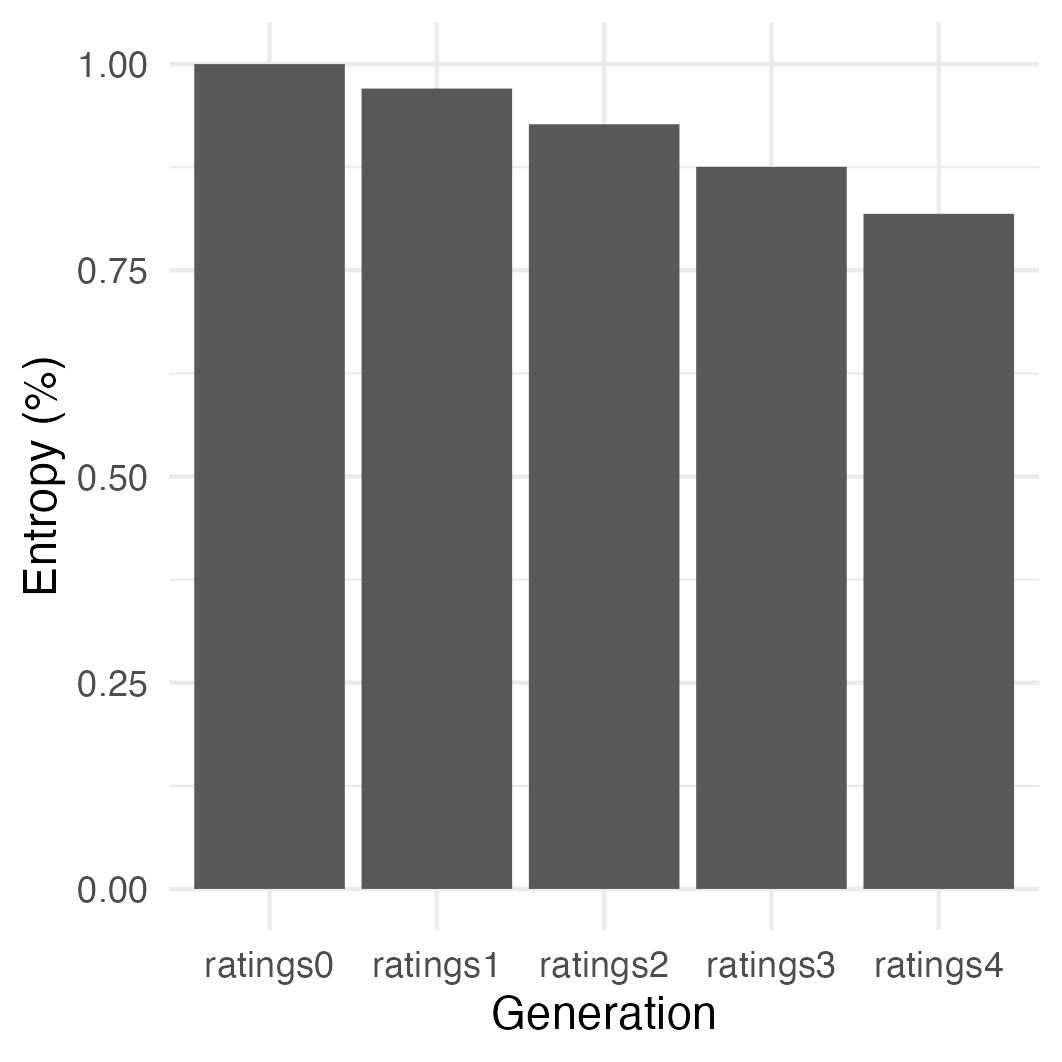
\includegraphics[width=\textwidth]{04_entropy}
  \end{subfigure}
  \caption{Recommendation entropy as a percentage of ratings0s entropy.
  \label{fig:fig04_entropy}}
\end{figure}

We can also observe this reduction of variety in an even more visual way. In
Figure~\ref{fig:fig04_popularity_time_both} we plotted movie popularity over
time; each line represents a movie and each step in the x-axis is a new
generation of the model. Figure~\ref{fig:fig04_popularity_time} makes it very
clear that no more than 15 movies rose in popularity over the four generations
of the recommendation system, becoming orders of magnitude more popular than the
rest. We also scaled the y-axis by taking the its log in
Figure~\ref{fig:fig04_log_popularity_time}, and we can see that, in fact, no
other movie rose in popularity besides the ones that stick out after
\verb|model2|.

It is also of note that the few movies that rise in popularity are not the most
popular ones from \verb|ratings0|, even though genre was the only metadata we
fed into the system. This uncovers a significant feature of the feedback loop we
observed in Figure~\ref{fig:fig04_profile_grouped}: the items that the algorithm
amplifies don't necessarily have to be the most mainstream, or in other words,
recommendation systems are able to boost content artificially.

\begin{figure}
  \centering
  \begin{subfigure}{0.45\textwidth}
    \centering
    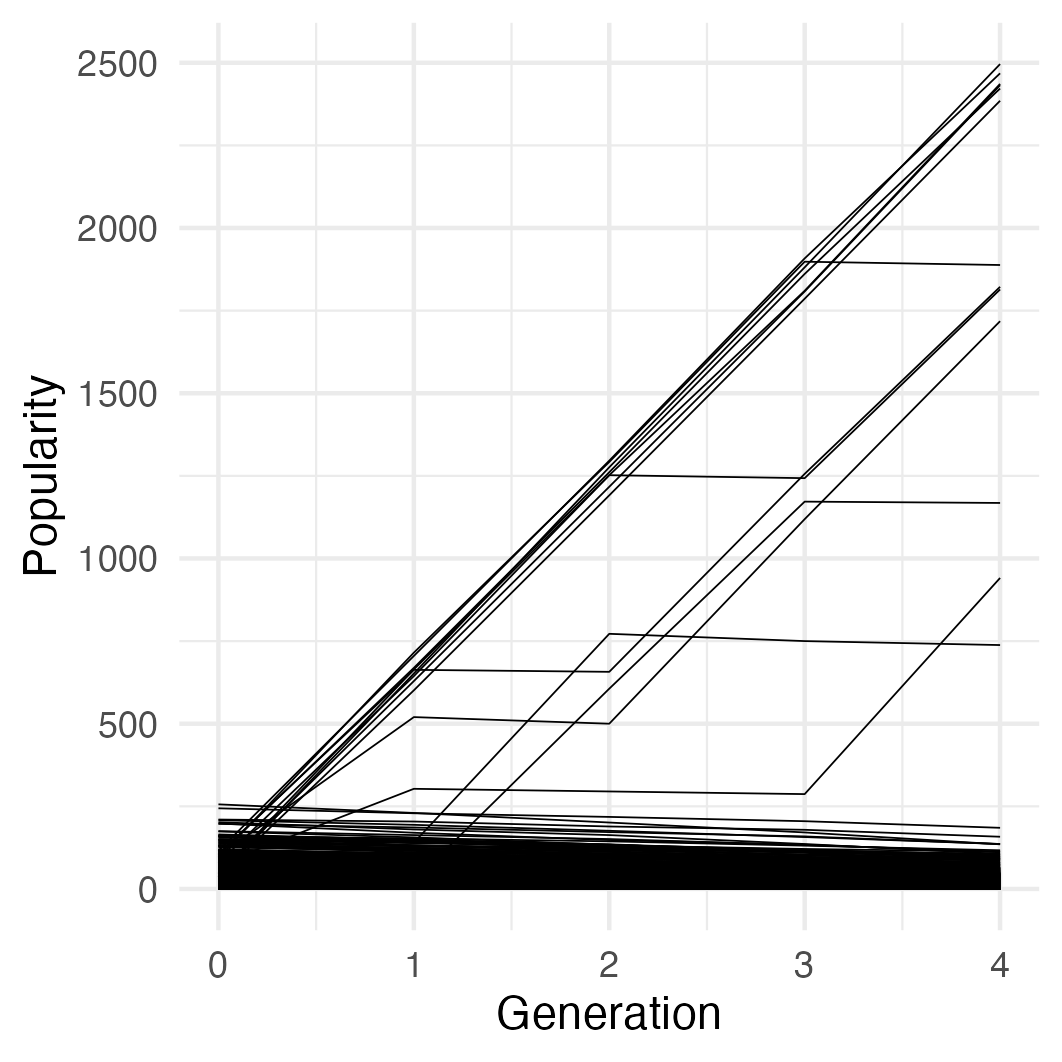
\includegraphics[width=\textwidth]{04_popularity_time}
    \caption{Movie popularity over time.\label{fig:fig04_popularity_time}}
  \end{subfigure}
  \begin{subfigure}{0.45\textwidth}
    \centering
    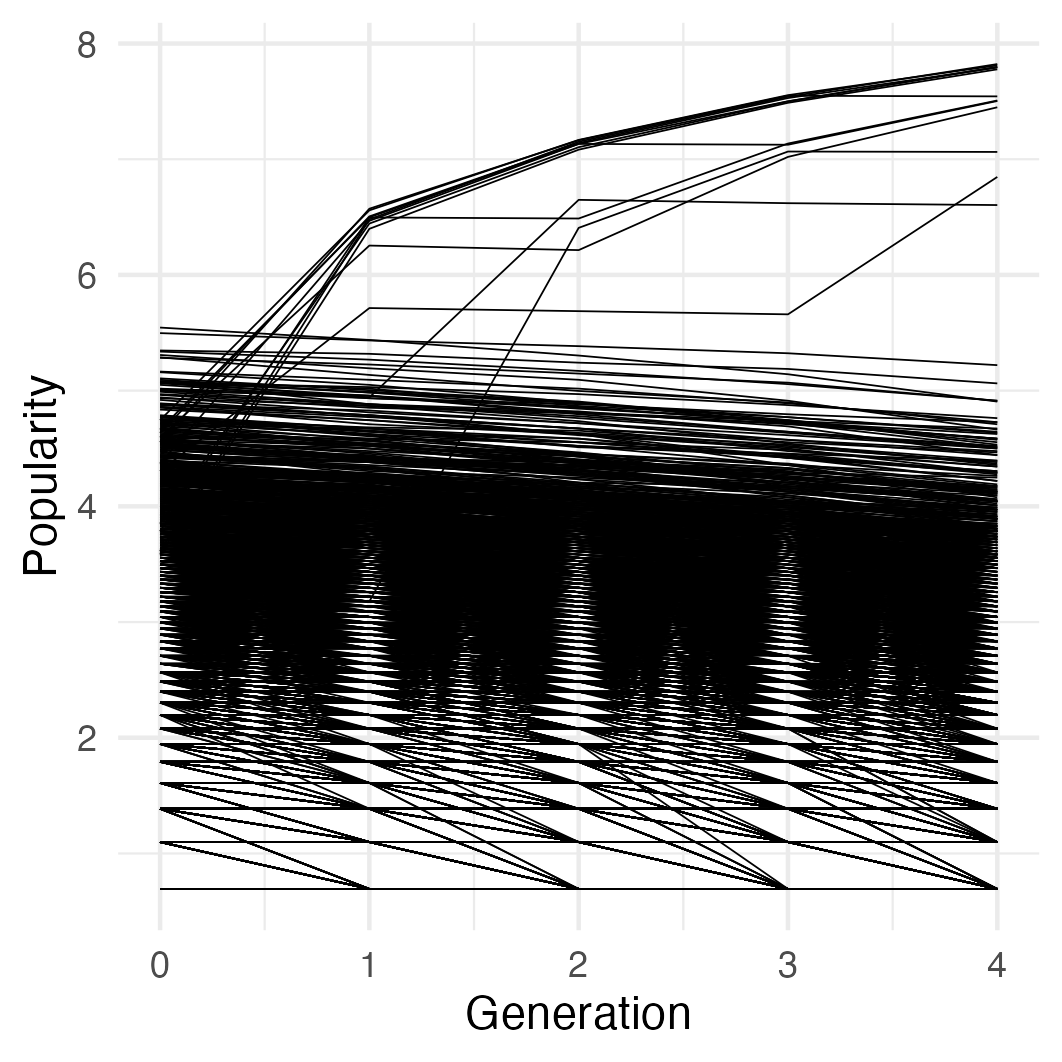
\includegraphics[width=\textwidth]{04_log_popularity_time}
    \caption{Movie log-popularity over time.\label{fig:fig04_log_popularity_time}}
  \end{subfigure}
  \caption{Popularity of every movie from ratings0 to ratings4.\label{fig:fig04_popularity_time_both}}
\end{figure}

\section{Modeling}
\label{sec:modeling04}

Having identified a feedback loop in the recommendation system, we decided to
fit a regression model on our generated data. The goal of this step is
essentially explainability \citep{}: to help better understand the algorithms
decisions.

% Computational Statistics do James E. Gentle

As is common in computational inference \citep{}, our process involved multiple
rounds of modeling. We started with a very simple model and, according to
goodness-of-fit measurements, made it more and more complex in order to achieve
a better representation of the behavior of the recommendation system. As we will
see later, even after feeding all of the the available data (and some extra
metadata that the recommender algorithm didn't have access to), our models were
not able to capture such a degenerate distribution.

The first model we attempted to use was a simple Poisson regression \citep{}.
Since the recommendation profiles displayed a strong positive skew and an
exponential-like decay, a log-linear model seemed like a good starting point.
For this kind of model \citep{}, we take a set of $\mathbf{x} \in
\mathbb{R}^{n}$ and fit a regression of the form

$$
\log(\operatorname{E} (Y \mid \mathbf{x})) = \alpha + \mathbf{\beta}'\mathbf{x},
$$

where $\alpha \in \mathbb{R}$ and $\mathbf{\beta} \in \mathbb{R}^{n}$. More
concretely, we used R's \verb|glm()| \citep{} function with the following
formula: \verb|pop ~ t * genre * rating|. In this expression, \verb|pop|
represents the popularity of a movie, \verb|t| represents the generation i.e.
the iteration from 0 to 4, and \verb|genre| represents the genre.

As the reader might be able to see, we used the genre variable in our regression
model even though we didn't feed it to the recommendation system. As explained
before, the algorithm only had access to the popularity and ratings of the
movies, but it is possible the there exists a latent effect of genre on the
other variables; since a machine learning system is much more flexible than a
regression model, we opted to explicitly feed the genre into the Poisson model
and all others that followed.

For illustrative purposes, we will present the full output of this model below.
It is notable how many coefficients are considered highly significant, meaning
that, individually, they were able to capture the feedback loop generated by
the recommendation system.

\begin{verbatim}
Call:
glm(formula = pop ~ t * genre * rating, family = "poisson", data = features)

Deviance Residuals:
    Min       1Q   Median       3Q      Max
-33.145   -3.088   -1.222    1.260   93.001

Coefficients:
                            Estimate Std. Error z value Pr(>|z|)
(Intercept)                9.210e-02  9.514e-02   0.968 0.333031
t                         -6.844e-02  4.200e-02  -1.629 0.103208
genreAnimation            -2.276e+00  1.475e-01 -15.430  < 2e-16 ***
genreChildren's            1.489e-02  1.754e-01   0.085 0.932347
genreComedy               -1.904e-01  1.041e-01  -1.828 0.067539 .
genreCrime                -4.898e+00  1.858e-01 -26.364  < 2e-16 ***
genreDocumentary          -1.801e+00  4.491e-01  -4.010 6.07e-05 ***
genreDrama                -1.035e+00  1.140e-01  -9.086  < 2e-16 ***
genreFilm-Noir            -1.631e+01  5.403e-01 -30.185  < 2e-16 ***
genreHorror                3.012e-01  1.178e-01   2.556 0.010582 *
genreMusical              -2.784e+00  4.813e-01  -5.784 7.31e-09 ***
genreMystery              -4.849e+00  2.464e-01 -19.681  < 2e-16 ***
genreRomance              -1.476e+00  5.299e-01  -2.785 0.005347 **
genreSci-Fi                1.583e+00  1.898e-01   8.341  < 2e-16 ***
genreThriller              3.854e-01  1.791e-01   2.152 0.031394 *
genreWestern              -4.253e+00  5.017e-01  -8.476  < 2e-16 ***
rating                     8.877e-01  2.740e-02  32.395  < 2e-16 ***
t:genreAnimation          -3.139e+00  6.223e-02 -50.435  < 2e-16 ***
t:genreChildren's         -5.212e-04  7.760e-02  -0.007 0.994641
t:genreComedy             -2.235e-02  4.602e-02  -0.486 0.627215
t:genreCrime              -3.561e+00  8.570e-02 -41.557  < 2e-16 ***
t:genreDocumentary         2.463e-01  1.933e-01   1.274 0.202583
t:genreDrama              -1.845e+00  5.015e-02 -36.799  < 2e-16 ***
t:genreFilm-Noir          -5.419e+00  1.944e-01 -27.872  < 2e-16 ***
t:genreHorror              7.776e-03  5.217e-02   0.149 0.881511
t:genreMusical             1.190e-01  2.140e-01   0.556 0.578236
t:genreMystery            -3.676e+00  1.032e-01 -35.632  < 2e-16 ***
t:genreRomance            -8.909e-02  2.334e-01  -0.382 0.702658
t:genreSci-Fi             -2.251e+00  8.076e-02 -27.869  < 2e-16 ***
t:genreThriller            6.362e-02  7.894e-02   0.806 0.420240
t:genreWestern             5.290e-02  2.211e-01   0.239 0.810874
t:rating                  -1.584e-02  1.212e-02  -1.307 0.191193
genreAnimation:rating      7.049e-01  3.938e-02  17.900  < 2e-16 ***
genreChildren's:rating    -4.814e-02  5.303e-02  -0.908 0.364006
genreComedy:rating         1.711e-02  2.989e-02   0.572 0.567055
genreCrime:rating          1.261e+00  4.818e-02  26.161  < 2e-16 ***
genreDocumentary:rating    5.638e-02  1.160e-01   0.486 0.626776
genreDrama:rating          1.163e-01  3.199e-02   3.635 0.000278 ***
genreFilm-Noir:rating      3.865e+00  1.239e-01  31.197  < 2e-16 ***
genreHorror:rating        -1.456e-01  3.541e-02  -4.111 3.95e-05 ***
genreMusical:rating        6.395e-01  1.255e-01   5.095 3.50e-07 ***
genreMystery:rating        1.286e+00  6.114e-02  21.030  < 2e-16 ***
genreRomance:rating        3.492e-02  1.506e-01   0.232 0.816639
genreSci-Fi:rating        -5.037e-01  5.457e-02  -9.230  < 2e-16 ***
genreThriller:rating      -1.952e-01  5.094e-02  -3.833 0.000127 ***
genreWestern:rating        9.773e-01  1.309e-01   7.467 8.19e-14 ***
t:genreAnimation:rating    8.263e-01  1.631e-02  50.671  < 2e-16 ***
t:genreChildren's:rating  -1.370e-03  2.350e-02  -0.058 0.953503
t:genreComedy:rating       6.194e-03  1.323e-02   0.468 0.639610
t:genreCrime:rating        9.129e-01  2.163e-02  42.204  < 2e-16 ***
t:genreDocumentary:rating -5.843e-02  5.002e-02  -1.168 0.242813
t:genreDrama:rating        5.028e-01  1.399e-02  35.927  < 2e-16 ***
t:genreFilm-Noir:rating    1.279e+00  4.402e-02  29.061  < 2e-16 ***
t:genreHorror:rating      -6.526e-03  1.573e-02  -0.415 0.678237
t:genreMusical:rating     -3.530e-02  5.588e-02  -0.632 0.527603
t:genreMystery:rating      9.553e-01  2.495e-02  38.291  < 2e-16 ***
t:genreRomance:rating      3.023e-02  6.624e-02   0.456 0.648140
t:genreSci-Fi:rating       6.707e-01  2.195e-02  30.551  < 2e-16 ***
t:genreThriller:rating    -1.870e-02  2.252e-02  -0.830 0.406351
t:genreWestern:rating     -1.209e-02  5.768e-02  -0.210 0.834031
---
Signif. codes:  0 ‘***’ 0.001 ‘**’ 0.01 ‘*’ 0.05 ‘.’ 0.1 ‘ ’ 1

(Dispersion parameter for poisson family taken to be 1)

    Null deviance: 562028  on 13559  degrees of freedom
Residual deviance: 268737  on 13500  degrees of freedom
AIC: 318813

Number of Fisher Scoring iterations: 6
\end{verbatim}

However, analyzing the coefficients by themselves is only one part of the full
picture. We used a simulation envelope \citep{} to assess global
goodness-of-fit, which is obtained by plotting the ordered absolute values of a
model diagnostic versus the expected order statistic of a normal distribution
\citep{}:

$$
\Phi^{-1}(\frac{i+3/8}{n+1/4})
$$

% Reescrever os 2 parágrafos abaixo. Eles foram tirados direto dos docs da
% hnp::hnp()

% Atkinson (1985)
\citet{} proposed the addition of a simulated envelope, which is such that under
the correct model the plot for the observed data is likely to fall within the
envelope. The objective is not to provide a region of acceptance, but some sort
of guidance to what kind of shape to expect.

Obtaining the simulated envelope is simple and consists of (1) fitting a model;
(2) extracting model diagnostics and calculating sorted absolute values; (3)
simulating 99 (or more) response variables using the same model matrix, error
distribution and fitted parameters; (4) fitting the same model to each simulated
response variable and obtaining the same model diagnostics, again sorted
absolute values; (5) computing the desired percentiles (e.g., 2.5 and 97.5) at
each value of the expected order statistic to form the envelope.

The resulting simulated envelope was generated with the \verb|hnp| \citep{} R
package and can be seen in Figure~\ref{fig:fig04_residual_poisson}. It is plain
to see that the model does not conform to the delimited region and, therefore,
isn't able to properly capture the variability of the data.

\begin{figure}
  \centering
  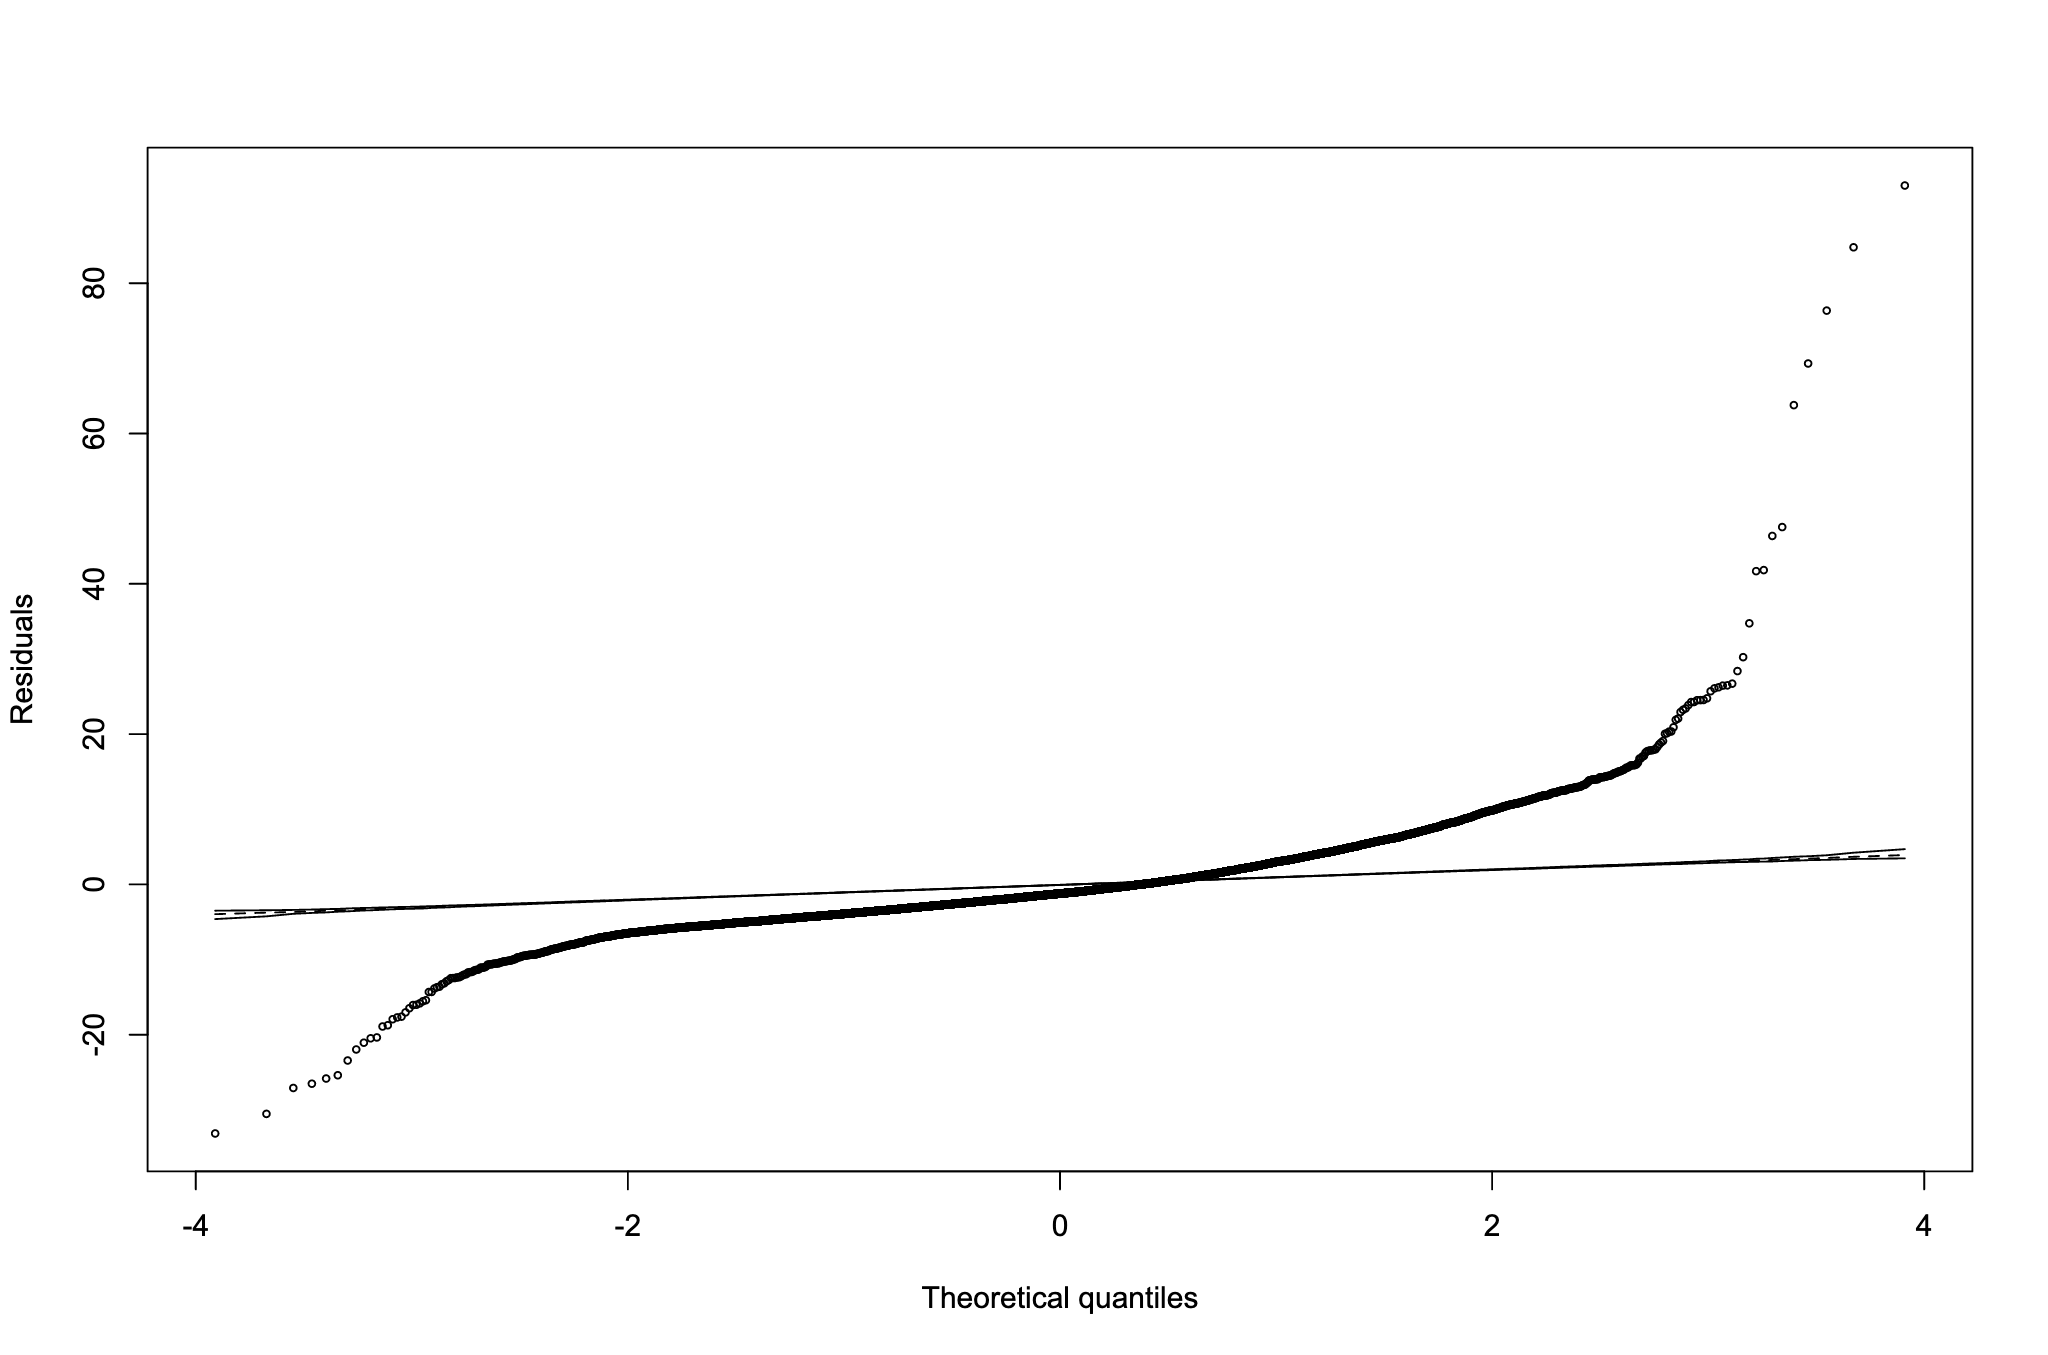
\includegraphics[width=\textwidth]{04_residual_poisson}
  \caption{Residual analysis via simulated envelope for the Poisson regression.\label{fig:fig04_residual_poisson}}
\end{figure}




..., and \verb|movie_id| is the ID of a movie. Note
that the genre was not used when training the recommendation models described
above, but it turned out that this feature could explain a lot of the models'
outputs.

\begin{verbatim}
  Family: nbinom2  ( log )
Formula:          pop ~ t * genre * rating + (1 | movie_id)
Data: features

     AIC      BIC   logLik deviance df.resid
 83863.8  84370.3 -41865.9  83731.8    15844

Random effects:

Conditional model:
 Groups   Name        Variance Std.Dev.
 movie_id (Intercept) 1.364    1.168
Number of obs: 15910, groups:  movie_id, 3182

Dispersion parameter for nbinom2 family ():   49

Conditional model:
                            Estimate Std. Error z value Pr(>|z|)
(Intercept)                -0.108714   0.272464  -0.399 0.689891
t                          -0.210272   0.021153  -9.941  < 2e-16 ***
genreAdventure              0.112129   0.574197   0.195 0.845174
genreAnimation             -2.286362   0.773873  -2.954 0.003132 **
genreChildren's             0.855196   0.755919   1.131 0.257915
genreComedy                -0.108159   0.352431  -0.307 0.758925
genreCrime                 -3.590470   0.850227  -4.223 2.41e-05 ***
genreDocumentary           -1.659325   1.508329  -1.100 0.271285
genreDrama                 -1.219969   0.409312  -2.981 0.002877 **
genreFilm-Noir            -16.633103   2.371128  -7.015 2.30e-12 ***
genreHorror                 0.512807   0.443025   1.158 0.247062
genreMusical               -4.259252   2.088483  -2.039 0.041410 *
genreMystery               -4.646920   1.461852  -3.179 0.001479 **
genreRomance               -2.118789   1.856289  -1.141 0.253699
genreSci-Fi                 0.363380   1.044431   0.348 0.727899
genreThriller               1.382908   0.855392   1.617 0.105944
genreWestern               -3.766758   2.108848  -1.786 0.074072 .
rating                      0.957533   0.085468  11.203  < 2e-16 ***
t:genreAdventure            0.161327   0.053403   3.021 0.002520 **
t:genreAnimation           -0.392012   0.067698  -5.791 7.01e-09 ***
t:genreChildren's           0.116028   0.066946   1.733 0.083068 .
t:genreComedy               0.119502   0.030504   3.918 8.94e-05 ***
t:genreCrime               -0.146821   0.085503  -1.717 0.085952 .
t:genreDocumentary          0.329357   0.195776   1.682 0.092507 .
t:genreDrama                0.005393   0.038739   0.139 0.889287
t:genreFilm-Noir           -0.730742   0.227275  -3.215 0.001303 **
t:genreHorror               0.148203   0.041813   3.544 0.000393 ***
t:genreMusical              0.265118   0.243060   1.091 0.275383
t:genreMystery             -1.150785   0.123034  -9.353  < 2e-16 ***
t:genreRomance              0.064921   0.227735   0.285 0.775590
t:genreSci-Fi              -0.311108   0.079779  -3.900 9.63e-05 ***
t:genreThriller             0.134758   0.077077   1.748 0.080403 .
t:genreWestern              0.184582   0.216581   0.852 0.394073
t:rating                    0.029594   0.006273   4.717 2.39e-06 ***
genreAdventure:rating      -0.209253   0.179840  -1.164 0.244606
genreAnimation:rating       0.594327   0.226301   2.626 0.008633 **
genreChildren's:rating     -0.473591   0.247951  -1.910 0.056131 .
genreComedy:rating         -0.194909   0.109223  -1.785 0.074341 .
genreCrime:rating           0.736375   0.243050   3.030 0.002448 **
genreDocumentary:rating    -0.113489   0.399299  -0.284 0.776242
genreDrama:rating          -0.031020   0.120957  -0.256 0.797601
genreFilm-Noir:rating       3.958891   0.595316   6.650 2.93e-11 ***
genreHorror:rating         -0.422452   0.151685  -2.785 0.005352 **
genreMusical:rating         0.944897   0.569196   1.660 0.096903 .
genreMystery:rating         1.092607   0.409047   2.671 0.007560 **
genreRomance:rating         0.013712   0.548422   0.025 0.980053
genreSci-Fi:rating         -0.423339   0.324094  -1.306 0.191477
genreThriller:rating       -0.729129   0.256016  -2.848 0.004400 **
genreWestern:rating         0.725673   0.578412   1.255 0.209625
t:genreAdventure:rating    -0.053250   0.015828  -3.364 0.000768 ***
t:genreAnimation:rating     0.110189   0.018603   5.923 3.16e-09 ***
t:genreChildren's:rating   -0.039499   0.020922  -1.888 0.059031 .
t:genreComedy:rating       -0.039790   0.008913  -4.464 8.04e-06 ***
t:genreCrime:rating         0.038460   0.022654   1.698 0.089557 .
t:genreDocumentary:rating  -0.088874   0.050610  -1.756 0.079076 .
t:genreDrama:rating        -0.006800   0.010754  -0.632 0.527202
t:genreFilm-Noir:rating     0.183567   0.054187   3.388 0.000705 ***
t:genreHorror:rating       -0.052874   0.013574  -3.895 9.81e-05 ***
t:genreMusical:rating      -0.082105   0.063538  -1.292 0.196285
t:genreMystery:rating       0.335177   0.032553  10.296  < 2e-16 ***
t:genreRomance:rating      -0.018634   0.064877  -0.287 0.773939
t:genreSci-Fi:rating        0.108210   0.023442   4.616 3.91e-06 ***
t:genreThriller:rating     -0.044310   0.022584  -1.962 0.049758 *
t:genreWestern:rating      -0.055461   0.056878  -0.975 0.329521
---
Signif. codes:  0 '***' 0.001 '**' 0.01 '*' 0.05 '.' 0.1 ' ' 1
\end{verbatim}

\begin{figure}
  \centering
  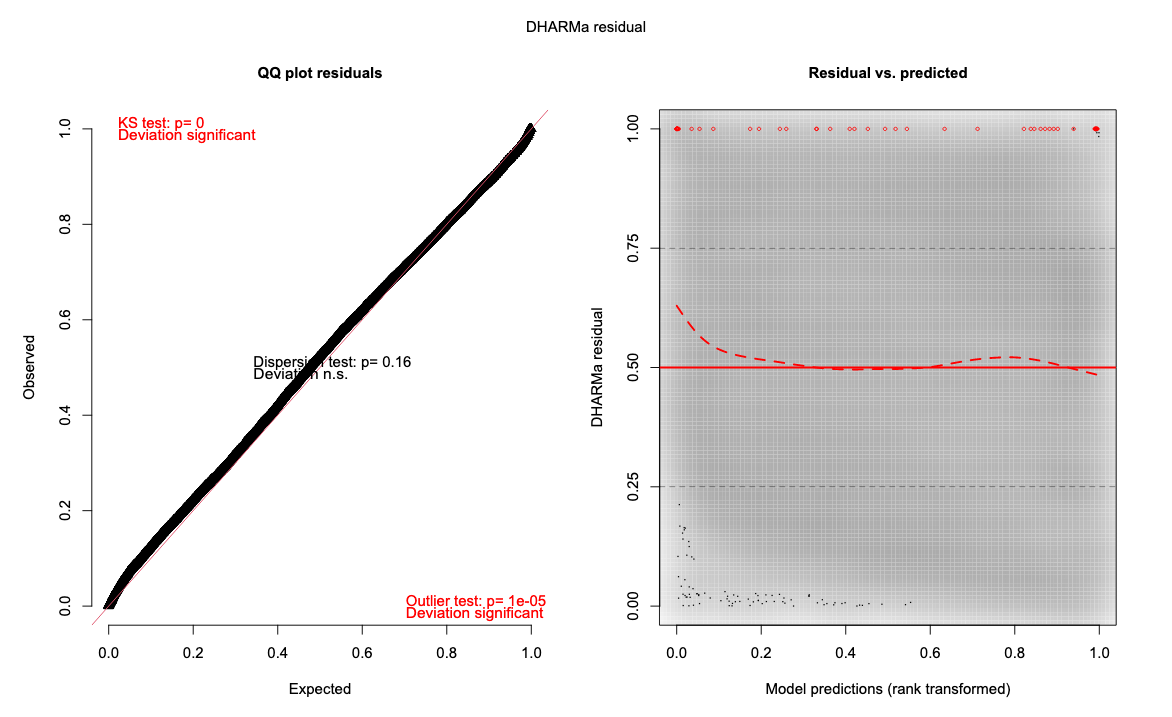
\includegraphics[width=\textwidth]{04_residual_mmnb2}
  \caption{Residual analysis for glmmTMB model.\label{fig:fig04_residual_mmnb2}}
\end{figure}

\par

%!TeX root=../tese.tex
%("dica" para o editor de texto: este arquivo é parte de um documento maior)
% para saber mais: https://tex.stackexchange.com/q/78101/183146

\chapter{Conclusion}
\label{cap:conclusion}

In this work, we studied recommender system bias. As detailed in
Chapter~\ref{cap:introduction}, these algorithms are pervasive in modern live
and have significant impact on our information diet; however, a growing body of
evidence indicates that these systems, specially when deployed in large social
networks, can display significant biases in their recommendations. Researchers
and activists alike worry that these biases might create echo chambers and
radicalization pipelines by amplifying extremist content. In broad terms, our
goal was to study one way through which these algorithms might be boosting
fringe viewpoints and radicalizing users: degenerate feedback loops.

Degeneracy in recommender systems has been explored before by
\citet{nguyen_exploring_2014} and \citet{jiang_degenerate_2019}. They concluded
that these algorithms show a tendency to reduce the diversity of recommended
content over time because of the feedback loop that occurs when the system must
learn from the its own outputs. Our main research objective was to further
characterize and model this behavior using both qualitative and quantitative
methods.

In Chapter~\ref{cap:review}, we reviewed the scientific literature that deals
with this topic and presented a few different viewpoints on the matter. Works by
\citet{hosseinmardi_evaluating_2020}, \citet{huszar_algorithmic_2021}, and
others suggest that social networks tend to amplify far-right views, while
\citet{munger_right-wing_2020} and \citet{ledwich_algorithmic_2019} posit that
this is not the case. \citet{ribeiro_auditing_2020} found evidence that, in
general, YouTube users tend to migrate from "lighter" content towards more
extreme videos, and \citet{stoica_algorithmic_2018} coined the term
``algorithmic glass ceiling'' to describe recommender system's propensity to
reinforce homophilic behavior.

We also drew attention to non-scientific endeavors that attempt to better
understand filter bubbles, echo chambers, and their impacts on the public. While
this issue is being debated in academia, journalists and whistleblowers like
\citet{ribeiro_como_2021} or \citet{wong_how_2021} hold social media companies
accountable by gathering anecdotal evidence and personal accounts about
algorithmic bias.

Our main contributions come in Chapters~\ref{cap:static} and \ref{cap:dynamic},
where we describe and conduct multiple experiments on recommender algorithms.

% Ver o que foi escrito em 2022 e colocar aqui para não ser pego de surpresa

\section{Static Analysis}
\label{sec:static}

Chapter~\ref{cap:static} started with a question: can recommender systems send
users in radicalization spirals? Given the many limitations of social media
analysis, we argue that the best way to answer this question is to explore the
simplest and most bare-bones algorithm possible. Our hypothesis is that, if such
a simple algorithm displays a feedback loop dynamic, then there might be some
intrinsic property of this type of system that pushes recommendations towards
degeneracy.

We designed multiple experiments with the goal of analyzing the recommendation
profile of our algorithm of choice: a simple, content-based recommender that
used cosine similarity as its internal metric. Recommendation profile is a
concept we developed as a shorthand for an algorithm's characteristic tendency
to recommend more frequently a smaller (or larger) subset of the original data.

Our expectation was that a systems's recommendation profile would be
approximately the same as the original dataset's item popularity distribution;
users that enjoyed less popular movies would be recommended other unpopular
items and users that enjoyed the more popular movies would likewise be
recommended other prominent items. This, however, was not the case.

In the original MovieLens \citep{harper_movielens_2015} dataset, the popularity
distribution was sub-exponential, meaning that there was not a sharp decrease in
the number of reviews from the most popular movies to the least popular ones.
This was in stark contrast to our vanilla model's exponential recommendation
profile. Figure ~\ref{fig:fig05_profile_comparison} displays the two profiles
side-by-side for ease of reference.

\begin{figure}
  \centering
  \begin{subfigure}{0.45\textwidth}
    \centering
    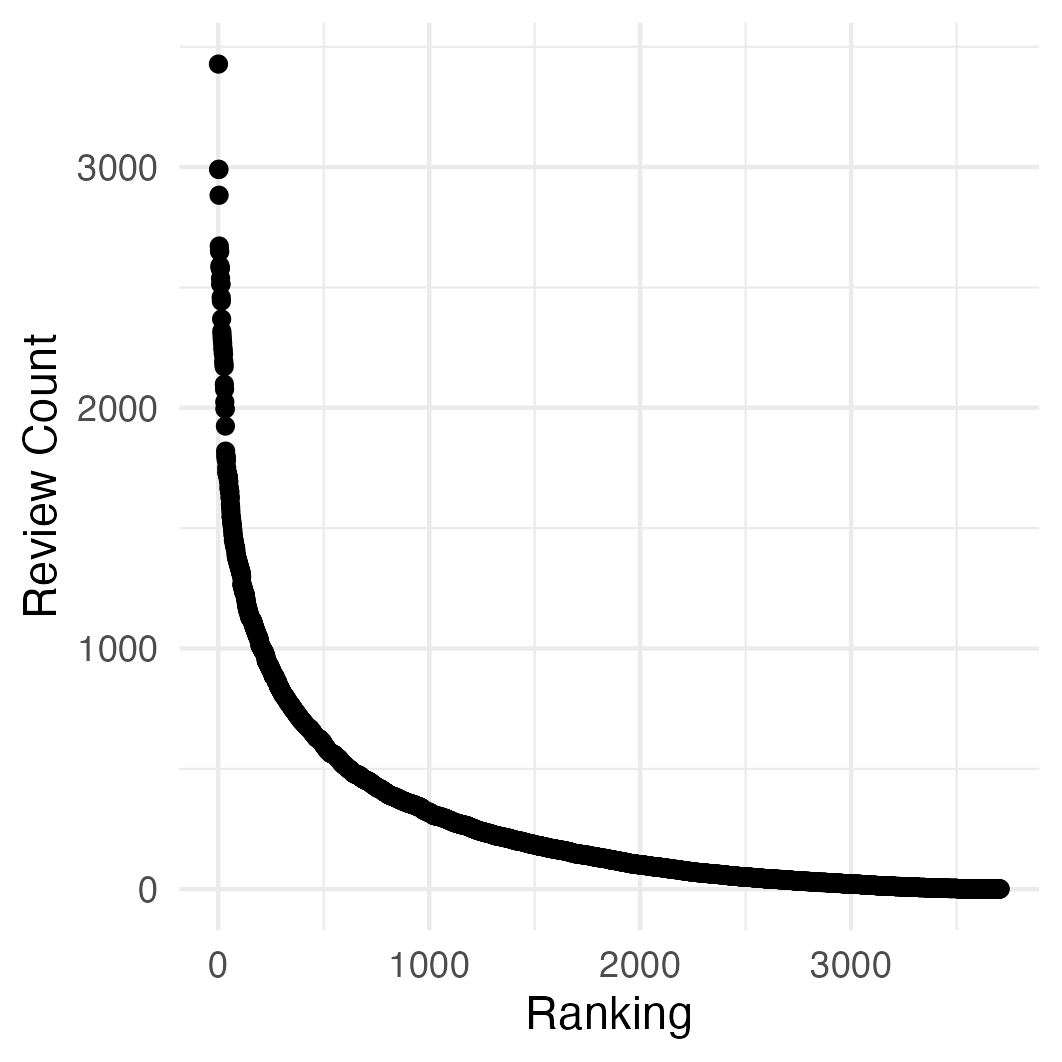
\includegraphics[width=\textwidth]{03_review_profile}
    \caption{Popularity distribution.\label{fig:fig05_review_profile}}
  \end{subfigure}
  \begin{subfigure}{0.45\textwidth}
    \centering
    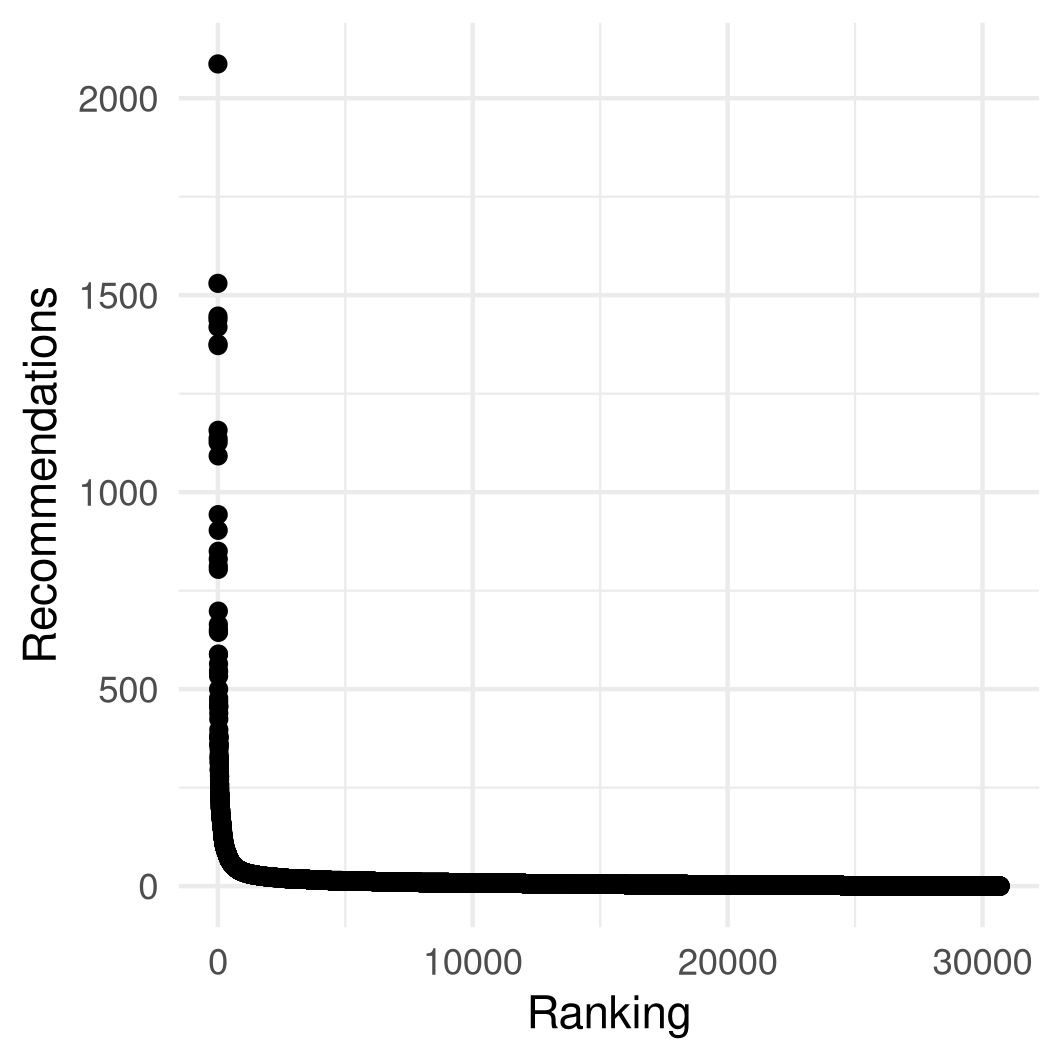
\includegraphics[width=\textwidth]{2a_vanilla}
    \caption{Recommendation profile.\label{fig:fig05_vanilla_profile}}
  \end{subfigure}
  \caption{Comparison between the original dataset's review profile (a) and the
  vanilla algorithm's recommendation
  profile.\label{fig:fig05_profile_comparison}}
\end{figure}

We experimented on many variations to the vanilla model and of the original
dataset, but all of them displayed exponential or super-exponential
recommendation profiles. This led us to posit that, indeed, recommender systems
might be prone to artificially amplifying some contents independently of the
original data. However, this static analysis was only part of the story and, in
order to confirm this hypothesis, we needed to take user dynamics into account.

\section{Dynamic Analysis}
\label{sec:dynamic}

We followed up the static experiments with a dynamic analysis. The main
question that motivated Chapter~\ref{cap:dynamic} was whether the amplification
pipeline detected in Chapter~\ref{cap:static} would be even further emphasized
by the interaction between user and recommendation system.

Even though we used a bare-bones algorithm again, this time we went with
Google's own machine learning library: TensorFlow Recommenders
\citep{noauthor_tensorflow_nodate}. Our goal was to capture the dynamics that
arise when a machine learning system has to learn from its own data, i.e., the
engagement of a user with items recommended by the algorithm itself. Since we
needed to generalize our conclusions to the environment of a social network, the
library Google uses to build its recommendation engines was the ideal choice.

Using the same MovieLens \citep{harper_movielens_2015} dataset, we created a
loop where the system would recommend 10 movies to a simulated user, this user
would then chose one movie at random to "watch", and this interaction would be
fed back into the model as a new input. This process was repeated 5 times for
each user in the original dataset.

Just as with the static experiments, the recommendation profile of our algorithm
got steeper and steeper over time, resulting in a similar super-exponential
decay; a diminishing set of movies was being recommended to a growing number of
users (as can be seen in Figure~\ref{fig:fig05_amplification}). Interestingly,
the movies that grew in popularity with time were not the most popular ones in
the original dataset.

In order to better understand the progression of the recommendation profile, we
tried to model this behavior using well-understood statistical distributions. If
we were able to accurately reproduce the results we obtained from the machine
learning algorithm with a white-box model, we would gain a deeper insight into
the internal mechanisms that caused the amplification pipeline we were
detecting.

\begin{figure}
  \centering
  \begin{subfigure}{0.45\textwidth}
    \centering
    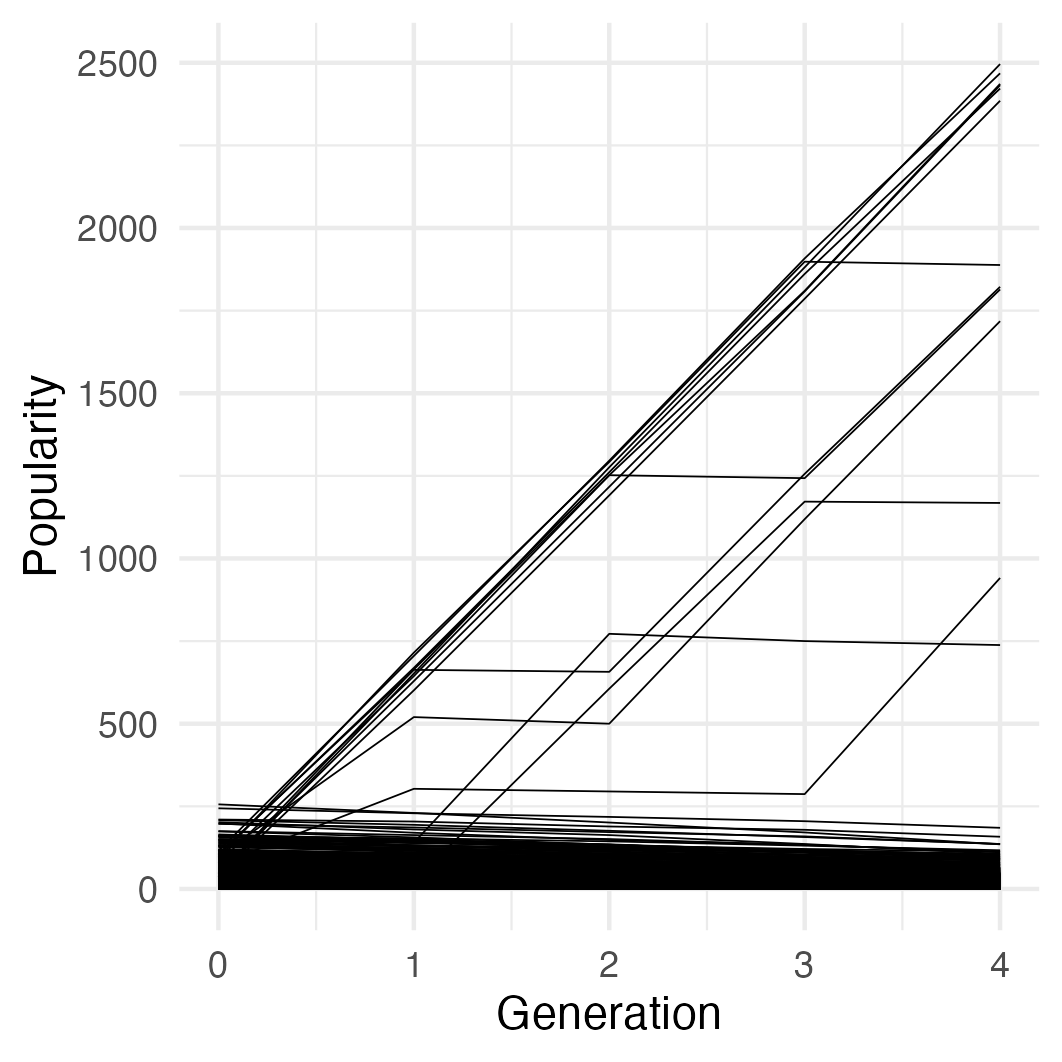
\includegraphics[width=\textwidth]{04_popularity_time}
    \caption{Movie popularity over time.\label{fig:fig05_popularity_time}}
  \end{subfigure}
  \begin{subfigure}{0.45\textwidth}
    \centering
    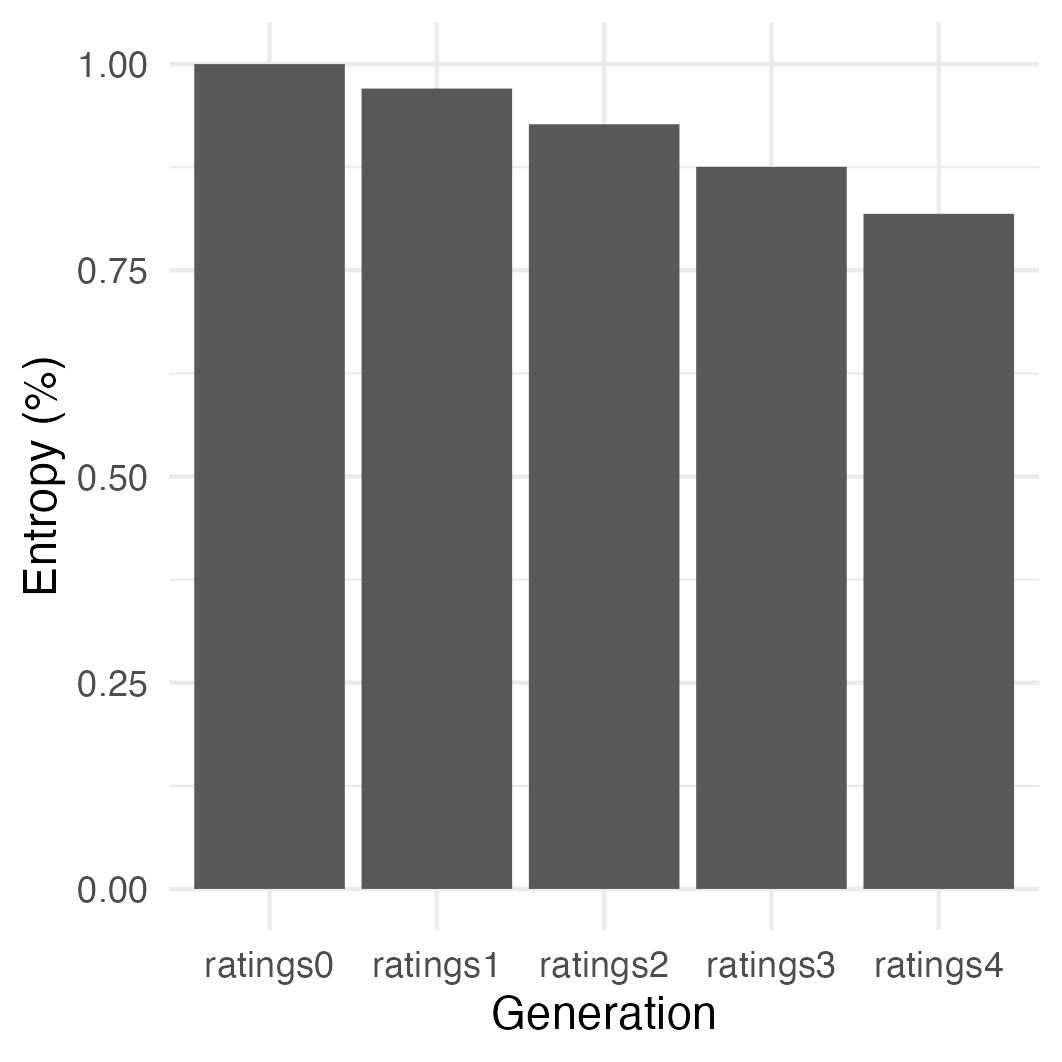
\includegraphics[width=\textwidth]{04_entropy}
    \caption{Recommendation entropy over time.\label{fig:fig05_entropy}}
  \end{subfigure}
  \caption{Amplification pipeline detected on the dynamic
  experiment.\label{fig:fig05_amplification}}
\end{figure}

We attempted to model the pipeline with Poisson and negative binomial
regressions, but had no success in both cases. We also tried adding
mixed-effects to these models and were better able to capture the variance of
the phenomenon, but a simulated envelope analysis revealed that our attempts
were still falling short.

As with the numbers obtained by \citet{} in a different scenario, the % Degenerate feedback loops in recommender systems
recommendation profiles of our model were tending quickly towards a degenerate
distribution. We believe that this is yet another piece of evidence that
suggests that recommender systems, if left unchecked, tent towards a confinement
dynamic where users' feeds devolve into filter bubbles and where the points of
view of highly-engaged minorities are amplified by a system that has to learn
from itself.

\section{Final Remarks}
\label{sec:remarks}

We began this work with the goal of developing a better understanding of the
mechanisms through which recommendation algorithms could be radicalizing users,
creating echo chambers and boosting fringe viewpoints. We believe we have found
enough evidence to support the hypothesis that recommender systems are able to
create amplification pipelines from degenerate feedback loops.

However, our findings are but one step in the direction of a solid theory.
Further research is still needed in order to find an unambiguous causal between
these processes and, more importantly, how to fix this behavior. A possible next
step would involve applying the methods discussed in this work to more complex
recommendation systems and to larger real-world datasets. Another possible
improvement would be to simulate users that ignore their recommendations.

\par

%!TeX root=../tese.tex
%("dica" para o editor de texto: este arquivo é parte de um documento maior)
% para saber mais: https://tex.stackexchange.com/q/78101/183146

% Os capítulos de compõem a dissertação/tese, com numeração normal, podem
% ser inseridos diretamente aqui ou "puxados" de outros arquivos.
% Em alguns (raros) casos, pode ser interessante usar \include ao
% invés de \input: https://tex.stackexchange.com/a/32058/183146
%!TeX root=../tese.tex
%("dica" para o editor de texto: este arquivo é parte de um documento maior)
% para saber mais: https://tex.stackexchange.com/q/78101/183146

%% ------------------------------------------------------------------------- %%
\chapter{Introduction}
\label{cap:introduction}

% Colocar uma prévia do trabalho em si, não só do contexto

Social networks have all but taken over contemporary daily life. From the
eponymous socializing, to reading news, to expressing ourselves, social media
has creeped into every corner of society. Most of its side-effects, it could be
argued, are positive (shortening distances, political accountability, social
organizing), but they are not perfect institutions.

Social media companies already face significant backlash for their questionable
business model and ethics. Cambridge Analytica's election meddling \citep{}, % Revealed: 50 million Facebook profiles harvested for Cambridge Analytica in major data breach
Facebook's subliminal experiments \citep{}, YouTube's problem with disturbing % Experimental evidence of massive-scale emotional contagion through social networks
content marketed at kids \citep{}, and Twitter's bot infestation \citep{} are % YouTube's latest hit: neon superheroes, giant ducks and plenty of lycra % Online Human-Bot Interactions: Detection, Estimation, and Characterization
just a few recent scandals that have put the societal role of social media into
question.

One particular controversy that has taken over public discourse around social
networks is the role that their algorithms might have in radicalizing users,
specially younger ones. The aforementioned experiments conducted by Facebook to
influence people's emotions and the proliferation of more than questionable
videos aimed at children on YouTube are instances that seem to corroborate the
notion that there is something fundamentally wrong with these companies'
algorithms.

News organizations, in general, have been skeptical of social networks.
Journalists and specialists alike argue that social media's algorithms
(specially recommender algorithms) are tuned to peddle conspiracy theories,
extremist views, and false information \citep{}. This would be the source cause % Mozilla Explains: Why Does YouTube Recommend Conspiracy Theory Videos?
for a plethora of what they consider contemporary evils: religious extremism,
anti-democratic leaders, widespread depression among teenagers, anti-science
movements, etc.

This narrative, of course, has been questioned for a variety of reasons. Some
say that it is self serving: traditional news organizations are being displaced
by social media and it would be convenient for them to mine the public's trust
in them \citep{munger_right-wing_2020}. Others claim that these recommender
algorithms are not to blame for political polarization and that social networks
even have a tendency to favor more left-wing viewpoints
\citep{ledwich_algorithmic_2019}.

The debate around the role of recommender systems in social media radicalization
is still, unfortunately, too recent and based in anecdotes. Since its impacts
are all but universal, more quality research is vital to inform both the public
and opinion makers about if and how much recommendation algorithms influence
social media users.

This dissertation aims to further such research.

\section{Social Networks}
\label{sec:social_networks}

Social networking services, also referred to as social networks and social
media, are notoriously difficult to define. Some definitions might be too narrow
(excluding instant messaging services), while some might be too broad (including
technologies such as telephone networks). Most definitions \citep{} include some % Social Network Sites: Definition, History, and Scholarship
common features:

\begin{itemize}
  \item Internet-based
  \item Focus on user-generated content
  \item Users have profiles
  \item Users can connect
\end{itemize}

While social-networking-like applications already existed in Usenet, Geocities,
launched in 1994, is usually regarded as the first major social network.
Friendster and Myspace followed in 2003, with Orkut and Facebook slightly
lagging behind in 2004. Each hit their peak at different moments and different
countries, but Facebook overtook all of them in 2009 when it became the most
popular social networking service in the world, still maintaining the title over
13 years latter at the moment of writing \citep{}. % Biggest social media platforms 2022

Even though all aforementioned social networks are multimedia, that is, users
can post text, photos and videos, some of the most popular services focus on a
specific type of media. For instance, YouTube (2009) centers around videos,
WhatsApp (2009) and WeChat (2011) were originally designed for text-based
communication, and Instagram's (2010) main focus is photos.

Parallel to all other features and idiosyncrasies, there lay the recommendation
algorithms. While a few social networking services (e.g. WhatsApp) do not
recommend any content or profiles to the user, most do and, according to recent
studies, these recommendations have become the main drivers of interactions
\citep{}. % acho que é um da stoica

\section{Recommender Systems}
\label{sec:recommender_systems}

Recommender systems (sometimes called recommendation systems or recommender
algorithms) first appeared in 1992 under the name ``collaborative filtering'',
even though that term nowadays refers to a subclass of recommender systems
\citep{goldberg_using_1992}. The aim of such an algorithm is providing users
with personalized product or service recommendations, an essential task when
considering the ever increasing number of possible videos to watch, music to
listen, products to buy.

The input of a recommender system is usually information about the preferences
(ratings, likes/dislikes, watch time, etc.) of consumers for a set of items.
Preference information can be gathered from explicit behaviors (e.g. rating a
product in a scale ranging from 0 to 5 stars) or from implicit behaviors (e.g.
how much time the user lingers on a product's page). These data can be combined
with information about the user (age, political leaning, etc.) in order to
create the best possible representation of the user's preferences.

The output of these systems can come in the form of a prediction or a list of
recommended items. In the first case, the goal of the algorithm is approximating
the rating a user would attribute to a yet unrated item, while the second type
of output involves gathering the items that most likely would interest the user.
Simple recommender systems that suggest items similar to the one being queried
do not necessarily involve rating predictions, but it is common to have the list
of recommended items based on the ratings the algorithms estimated the user
would give to those items.

Most recommender systems fall into one of four categories according to the
filtering algorithm they use, that it, the strategy for generating predictions
or selecting the top-N items: content-based filtering, demographic filtering,
collaborative filtering, and hybrid filtering
\citep{bobadilla_recommender_2013}.

Content-based filtering leverages characteristics of the content in order to
generate the recommendations \citep{ricci_introduction_2011}. One such algorithm
might use the genres of watched movies in order to recommend new ones, while
another might analyze the sound signature of a song to recommend similar ones,
but, either way, all content-based systems establish a similarity between items
as a basis for recommendations. Analogously, demographic filtering uses
demographic data to establish a similarity between users and recommend items
positively rated by similar people.

Collaborative filtering algorithms also recommend items that similar users
liked, but, in this case, the similarity between users is based on past ratings
and not demographic information \citep{ricci_introduction_2011}. Hybrid
filtering usually mix collaborative methods with either content-based or
demographic filtering \citep{ricci_introduction_2011}.

As with other knowledge-based systems, recommendation algorithms have quickly
incorporated neural networks and other machine learning techniques over the past
few years. Even though the implementation of YouTube's recommendation algorithm
is a trade secret, it is known to gather enormous amounts of data about the
user's interaction with the website and to require Google's own TPUs in order to
be trained. It also involves two distinct steps: candidate generation (when the
billions of videos available on the platform are quickly narrowed down to a few
hundreds that might be relevant) and ranking (when the algorithm actually
attempts to predict the score a user would implicitly give to the candidate
videos) \citep{}. % Improving Relevance Prediction with Transfer Learning in Large-scale Retrieval Systems

Another relevant aspect of recommender systems that is well-exemplified by
YouTube is the use of balancing factors such as novelty, dispersity, and
stability \citep{zhao_recommending_2019}. In the case of Google's video giant,
there is a baked-in bias for recency, strongly favoring newer videos in
detriment of older content \citep{zhao_recommending_2019}.

From this kind of bias stems much debate: as recommender systems explode in
popularity, so does research regarding its shortcommings. User radicalization
and algorithmic bias (explicitly programmed or not) are hotly debated subjects
in the literature.

\section{Radicalization and Bias}
\label{sec:radicalization_bias}

Opinion polarization is far from a recent phenomenon, and social media is only
the most recent communication medium where it can be detected and studied. An
important question is whether it facilitates or attenuates polarization:
anecdotal evidence might suggest that social network structures incentivize
users to gather into antagonistic communities, but this could be a result of
people simply being more likely to express their preferences online, not of some
intrinsic property of social media.

One possible byproduct of polarization is radicalization. Despite not being
entirely different phenomena, these concepts deserve distinct levels of
attention. While polarization can be considered a natural part of democratic
discourse, radicalization only happens when certain conditions are met. UNESCO
defines radicalization as \citep{seraphin_youth_2017}:

\begin{itemize}
  \item The individual person's search for fundamental meaning, origin and
        return to a root ideology;
  \item The individual as part of a group's adoption of a violent form of
        expansion of root ideologies and related oppositionist objectives;
  \item The polarization of the social space and the collective construction of
        a threatened ideal 'us' against 'them,' where the others are dehumanized
        by a process of scapegoating.
\end{itemize}

The third point is of special importance to the distinction between polarization
and radicalization. The first might be a simple consequence of democratic
disagreements between opposing parties, but the latter involves a dehumanization
of the opposition, which can lead to extremism: radicalism so intense that the
only effective strategy is physically exterminating the opposition.

Understanding how polarization might lead to radicalization (and, ultimately, to
extremism) is, therefore, of paramount significance to cultivate healthy
democracies, specially in the digital age. Since most social networks, as of
this writing, are still poorly moderated, they allow users to be exposed to a
plethora of viewpoints, from benign to insidious, possibly configuring a
``pipeline of radicalization'' through which regular users end up radicalized by
coming into contact with extreme content \citep{ribeiro_auditing_2020}.

Of course this argument is still very much open for debate. As will be shown in
Chapter~\ref{cap:review}, researchers have found evidences both for and against
the pipeline hypothesis and even proposed other means though which social media
might help radicalize users (e.g. the supply and demand hypothesis
\citep{munger_right-wing_2020}). Despite all disagreements, one common point
addressed by most research is the role of recommendation algorithms in serving
users with radicalizing content.

Proponents of the pipeline hypothesis, for instance, argue that recommendation
systems, aiming to maximize content consumption, suggest items that reinforce
preconceived notions of the user and that play on fear and paranoia
\citep{ribeiro_auditing_2020}. Content that appears urgent and leaves the user
fearful (for their live, their community, or their identity) could be more
engaging and, therefore, might be more susceptible to being considered as
relevant by the algorithm.

Even if the pipeline hypothesis is correct, specifics of how much algorithms are
to blame for radicalization are still unknown and hard to pin down. Most
research about the subject focuses on specific platforms (like Twitter and
YouTube) and have severe limitations with regards to how much data those
companies make available, not to mention the constant changes made to the
algorithms over the years that might alter their radicalization properties.
Definitive evidence for one theory or another must, therefore, apply to
recommender systems in general and be predictive of how they work both in
controlled and real life scenarios.

% mesclar parágrafo abaixo

YouTube, for example, currently has over 2 billion monthly logged-in users
\citep{}, but it makes no significant effort to clarify changes made to the % https://blog.youtube/press/
algorithm or even whether they fulfill their promises of reducing user exposure
to radicalizing content. With more than 500 hours of content being uploaded
every minute \citep{}, if 1\% of all videos can be considered radicalizing and % https://blog.youtube/press/
the algorithm can detect 99\% of them, that still leaves over 25.000 hours of
brand new extremist content free to spread on the platform every year. This goes
to show that, in the scale that these companies operate, even a small fraction
of content might still be enough to influence the overall recommendations made
by the algorithm. It is also worth noting that most of these platforms' efforts
are concentrated in their parent countries (usually the United States), so, even
if they actually try and remove the offending content, most of the
non-English-speaking world would still not be impacted by their policy changes.

Closely related to user radicalization is the subject of algorithmic bias.
YouTube, for example, has an explicit bias towards recency
\citep{covington_deep_2016}, meaning that more recent videos get "boosted" by
their recommendation algorithm. This is explicitly coded into the system, but
there are also implicit biases, learned by watching user behavior.

Stoica \citep{stoica_algorithmic_2018} studied Instagram profiles before and
after the implementation of their recommendation engine. They discovered that
male users had a slight predilection for following other men, while women
displayed no such preference and, as soon as the recommender system was
deployed, engagement with profiles of male users skyrocketed even though they
were the minority on the platform. The algorithm recognized and leveraged this
so called differentiated homophily effectively, but we might question whether or
not this should be the desired outcome of a good recommender system.

In social networks where recommendations are front and center, such as YouTube,
the algorithm could go from being a mere reflection of user preferences to
actively shaping user behavior. Hypothetically, a minoritary group of highly
engaged users with strong self-reinforcing consumption habits could tip the
scales of the algorithm and cause fringe content to be amplified; this is only
one way through which a radicalization pipeline could spontaneously form in a
social network.

% If this stuff happens at a sufficient scale (big % of the web), it could stop generative text models in their tracks -- their performance would degrade as they start training on their own output.

\section{Research Goals}
\label{sec:research_goals}

As explained in the previous sections, social networks' recommendation
algorithms might play a significant role in radicalizing users. This could be,
at least in part, be a result of implicit and explicit biases in recommender
systems.

This dissertation aims to explore the radicalization pipeline hypothesis and,
more specifically, understand the mechanisms through which recommender systems
can end up learning or developing biases. The research developed here revolves
around the dynamical properties of recommender systems (i.e., the sequence of
items suggested to an arbitrary user over time) and how feedback loops can
create ``amplification pipelines'' inside these engines.

In short, the main motivator of this research is to test the pipeline hypothesis
in a setting where recommendation algorithms learn dynamically.

\section{Outline}
\label{sec:outline}

...

\par

%!TeX root=../tese.tex
%("dica" para o editor de texto: este arquivo é parte de um documento maior)
% para saber mais: https://tex.stackexchange.com/q/78101/183146

\chapter{Literature review}
\label{cap:review}

There are three types of work that are relevant to the current topic: general
literature about recommender systems, evidences of algorithmic bias, and methods
of creating fairer recommendations. Since this area of study is still mostly
unexplored, there is no consensus on whether social media recommender systems
favor extremist content (or even whether they are actually deradicalisation
agents), which means that many references used in this work might disagree
amongst themselves.

\section{Scientific literature}
\label{cap:scientific}

General literature about recommendation algorithms is abound. One of the most
cited surveys was elaborated by \citet{bobadilla_recommender_2013}, but
works by \citet{he_interactive_2016} (about interactive recommender systems),
and by \citet{kunaver_diversity_2017} (about diversity in recommender systems)
were also used in order to draw a complete panorama of the field.

Another relevant article, by \citet{guy_social_2010}, is the landmark paper that
inaugurates the usage of user data alongside labels to create a recommendation
algorithm that is highly accurate and a staple of modern social networks. This
essentially starts the usage of recommenders systems in social media.

When talking specifically about YouTube's recommendation algorithms, two papers
deserve special attention. The first one, by \citet{covington_deep_2016}, marks
YouTube's move towards the usage of deep neural networks to generate video
recommendations. The authors describe a two-stage model that first generates a
list of candidates and then ranks them, also reporting dramatic performance
improvements. The second one, by \citet{zhao_recommending_2019}, describing a
more recent version of YouTube's recommendation algorithm, explores the
Multi-gate Mixture-of-Experts technique to optimize recommendations for more
than one ranking objective and the Wide \& Deep framework to mitigate selection
biases. The authors also make it clear that YouTube's recommender system has a
strong bias towards more recent content instead of more traditional metrics.

Many authors have also explored how biases in recommendation engines might lead
to user radicalization. \citet{agarwal_topic-specific_2015} developed an early
example of a technique to try and find extremist content on YouTube. Using
advanced machine learning methods, the authors create a YouTube crawler that
starts from a seed video and iteratively classifies featured channels and videos
according to their potential extremism. A more recent example of this can be
found in \citet{tangherlini_automated_2020}, where the authors propose a novel
approach for identifying conspiracy theories online. By analyzing the narrative
structure of a conspiracy theory (Pizzagate) and comparing it to an actual
conspiracy (Bridgegate), they create a model that can guess whether a
conspiratorial narrative is or not fabricated. According to their findings, a
multi-domain nature and the presence of keystone nodes are signs that strongly
indicate a conspiracy theory.

Besides just finding and identifying radicalizing content on YouTube, many
authors have been concerned with studying the radicalization dynamics directly.
\citet{alfano_technologically_2020}, for example, claim to be ``the first
systematic, pre-registered attempt to establish whether and to what extent the
recommender system tends to promote such [extremist] content.''
\citet{cho_search_2020} also attempt to understand how users can be radicalized
by the algorithm. By experimentally manipulating user search/watch history, the
authors concluded that algorithmically recommended content can reinforce a
participant's political opinions.

In the same vein, \citet{faddoul_longitudinal_2020}, after some high-profile
cases of users being radicalized through YouTube videos, studied the efforts
announced by the platform to curb the spread of conspiracy theories on the
website. The paper aimed to verify this claim by developing both an emulation of
YouTube's recommendation algorithm and a classifier that labeled whether a video
is conspiratorial or not. The authors describe an overall decrease in the number
of conspiracy recommendations, though not when weighing these recommendations by
views.

Three papers that deserve a closer look are those that investigate how regular
recommendation algorithms can learn covert biases in the users of a social
network and amplify them to previously unimaginable rates.
\citet{stoica_algorithmic_2018} explore the existence of an ``algorithmic glass
ceiling'' and introduces the concept of differentiated homophily. The authors
experiment on a Instagram dataset before and after the introduction of
algorithmic recommendations and discover that, even though most of that
network's users were female, the most followed profiles were male. They explain
this phenomenon by postulating that the algorithm learns biases in the
population, that is, male preference for male profiles (which doesn't happens
for females and thus characterizes an asymmetric---differentiated---homophily),
and ends up enhancing this effect. \citet{stoica_hegemony_2019}, building on top
of their previous work, create a proposal for new recommender systems that take
differentiated homophily into account in order to reduce the ``glass ceiling''
effect observed in non-corrected recommendation algorithms. The work focuses on
the theoretical description of the algorithm, but also attempts to validate its
hypothesis in real world data. \citet{stoica_algorithmic_2020}, in their most
recent paper, show that the most commonly used metrics in recommender systems
``exacerbate disparity between different communities'' because they reinforce
homophilic behavior of the network. This has profound implications, since these
algorithms might further suppress already minoritary viewpoints without being
explicitly programmed to do so.

Like the aforementioned articles, \citet{matakos_maximizing_2020} also propose a
novel recommendation algorithm that tries to strike a balance between
information spread and ensuring that the users are exposed to diverse
viewpoints. The authors show that this goal is important if we want to foster
healthy online debate, and that the algorithm is efficient and scalable with a
minor approximation. One possible inspiration for these papers might be one by
\citet{su_effect_2016} that studyed the network structure of Twitter before and
after the introduction of algorithmic recommendations (``Who to Follow''). The
authors of the paper discovered that all users benefitted recommendations, but
that users with already popular profiles benefitted even more, effectively
changing the network structure and dynamics. \citet{caton_fairness_2020} have
recently compiled other valuable information on fairness in machine learning
into a survey.

Because of data limitations, there still are few studies that investigate how
recommendation algorithms work dinamicaly, over time.
\citet{burke_evaluating_2010} point out that most methods for evaluating
recommender systems are static, that is, involve static snapshots of user and
item data. The authors propose a novel evaluation technique that helps provide
insight into the evolution of recommendation behavior: the ``temporal
leave-one-out'' approach. A more recent example of this approach was developed
by \citet{roth_tubes_2020}. Their paper delves into the confinement dynamics
possibly fostered by YouTube's recommendation algorithm. The authors create,
from a diverse set of seed videos, a graph of the videos iteratively recommended
by YouTube and, from this, study whether there were created ``filter bubbles''.
They find that indeed YouTubes recommendations are prone to confinement dynamics
be it topological, topical or temporal.

Even more recently, \citet{yao_measuring_2021} propose an approach for measuring
recommender system bias based on simulated users. Even though this work focuses
only on bias towards popular content, it is of particular importance because it
was written by researchers from Google itself. Some years before,
\citet{dash_network-centric_2019} also proposed a framework for auditing
recommender systems based on its network of users. Another contribution of their
work is a novel quantifications of diversity.

A different approach to understanding biases in recommendation algorithms range
from analyzing similarity metrics to developing theoretical bounded confidence
models. \citet{giller_statistical_2012} goes with the first strategy, and
identifies certain aspects of cosine similarity that are often overlooked.
Starting from simple theorems regarding the density of n-dimensional spheres,
the author concludes that the expected cosine similarity between random
bitstreams might be significantly different from the average. This is noteworthy
because many recommendation algorithms use cosine similarity in order to
determine the similarity between two items to recommend.
\citet{sirbu_algorithmic_2019} go with the latter, providing an interesting
theoretical model of how inherent biases in algorithmic recommendations might
highten opinion polarization. Using a bounded confidence model, the authors
propose the addition of a $\gamma$ term that represents the odds of an algorithm
recommending content that differs from that of a user.

Some recent papers also try to understand how YouTube might be favoring
right-wing and fascist content in specific, as opposed to trying to prove a more
general (and possibly less tractable) claim.
\citet{hosseinmardi_evaluating_2020} find evidence via a longitudinal study that
there exists ``a small but growing echo chamber of far-right content
consumption'' on YouTube. According to their research, these users are more
engaged than other, with YouTube generally accounting for a larger share of
their online news diet than the average. The authors, however, find no evidence
of this phenomenon being due to recommendations. A popular article in the field,
by \citet{ribeiro_auditing_2020}, explored the radicalization pipeline
hypothesis of algorithmic enabled radicalization. The authors collect huge
amounts of YouTube comment data over time, and determine a significant migration
of users from ``lighter'' content towards more extreme videos. This does not
prove that the pipeline exists, but is a strong argument for its existence.

Twitter was also found to consistently favor right-wing content.
\citet{huszar_algorithmic_2021} conducted a ''long-running, massive-scale
randomized experiment`` across 7 countries in order investigate the effects of
algorithmic personalization on users' feeds and, according to their results,
``mainstream political right enjoys higher algorithmic amplification than the
mainstream political left''.

Finally, feedback loops are of special interest to this discussion. Caused by
the inevitable fact that recommender systems must learn from users' reactions to
its own recommendations, they are a widely believed to be a powerful engine of
bias amplification and are discussed at length in the literature. Already in the
last decade, \citet{sinha_deconvolving_2017} investigated the viability of
identifying items affected by these feedback loops and attempted to created a
method of deconvolving them. More recently, \citet{jiang_degenerate_2019}
explored what they called ``degenerate feedback loops'' and their capability of
creating echo chambers, going as far as proposing a novel approach of slowing
down this tendency towards degeneracy. In a related study,
\citet{mansoury_feedback_2020} explored how recommender systems amplify already
popular content, but, more importantly, how this tendency might reduce content
diversity and cause users' tastes to shift over time. Depending on what a
systems values (recency, virality, controversy, engagement), this type of
feedback loop could possibly amplify not ``popular'' content, but divisive and
extremist content.

A minortiy of papers tries to disprove the hypothesis that social networks in
general, and YouTube in specific, have a radicalizing tendency.
\citet{munger_right-wing_2020} published a controversial article that postulates
a new model for YouTube radicalization. According to the authors, YouTube's
algorithm is not to blame, the users themselves are looking for extreme content
and the recommender system only supplies them. Its methods were highly
questioned by the community and is currently the only paper that spouses the
supply and demand hypothesis. \citet{ledwich_algorithmic_2019} also wrote a
highly controversial paper where its authors claim to have found evidence to
support the hypothesis that YouTube's recommendation algorithm favors mainstream
and left-leaning channels instead of right-wing ones. They categorize almost 800
channels into groups of similar political leaning and analyze recommentations
between each group, finding that YouTube might actually discourage users from
viewing radicalizing content. Most researchers though do not support the methods
employed by these two articles. In an even earlier study on news recommendations
of a major Dutch newspaper, \citet{moller_not_2018} claim that recommenders
systems had no significant impact on content diversity.

Even with a quickly growing body of research, further studies are needed in
order to shed more light into the inner workings of how recommendation
algorithms are used by social networks. Articles like the ones described in this
chapter are of utter importance to this task, but generalist studies that are
able to capture dynamics common to all or most recommender systems are still
nonexistent.

\section{Journalistic efforts}
\label{cap:journalistic}

Since this field of study is still in its infancy, many relevant sources are not
scientific in nature. Journalism, specially when investigative in nature, is a
valuable ally when trying to understand what is happening behind the curtains of
social platforms.

Some examples of journalistic endeavors that inform and guide scientific
research include, but are not limited to, a series by \citet{lecher_one_nodate}
on how different are Americans' Facebook feeds, a report (in Portuguese) by
\citet{ribeiro_como_2021} on how the far-right is still able to cheat YouTube's
attempts at curbing extremist content, and a whistleblower's account to
\citet{wong_how_2021} of how Facebook's executives resist on restricting
fake engagement that is able to distort global politics.

\par

%!TeX root=../tese.tex
%("dica" para o editor de texto: este arquivo é parte de um documento maior)
% para saber mais: https://tex.stackexchange.com/q/78101/183146

% Vamos definir alguns comandos auxiliares para facilitar.

% "textbackslash" é muito comprido.
% \newcommand{\sla}{\textbackslash}

% Vamos escrever comandos (como "make" ou "itemize") com formatação especial.
% \newcommand{\cmd}[1]{\textsf{#1}}

% Idem para packages; aqui estamos usando a mesma formatação de \cmd,
% mas poderíamos escolher outra.
% \newcommand{\pkg}[1]{\textsf{#1}}

% A maioria dos comandos LaTeX começa com "\"; vamos criar um
% comando que já coloca essa barra e formata com "\cmd".
% \newcommand{\ltxcmd}[1]{\cmd{\sla{}#1}}

\chapter{Static Analysis}
\label{cap:static}

Understanding how social networks recommend content to users is central to the
debate around political polarization and radicalization. There are many ways of
exploring recommender systems without examining their code, from simulating
their behavior after careful observation \citep{yao_measuring_2021} to directly
collecting recommendation data \citep{ribeiro_auditing_2020}, but most of them
allow us to examine only one perspective of the algorithm at a time. This means
that studying a social network's recommendation technique has inherent
limitations.

Most of the algorithms currently employed by social media companies are trade
secrets. They are also subject to constant experimentation and tuning
\citep{noauthor_congratulations_2020}, which might render worthless any research
performed before an update to the algorithm, no matter how careful the design of
the study was.

With our experiments we aim to make a tangible contribution to the field of
recommender systems, specifically how their design might (or might not) foster
confinement dynamics and create degenerate feedback loops. If it does, this
could mean that even a relatively small fraction of the content can tip the
algorithm in its favor, amplifying their message, creating filter bubbles, and
possibly sending users on a radicalization spiral if that topic is related to
politics or other contentious subjects.

In this chapter we will analyze a recommendation system statically, that is,
without taking into account its evolution after multiple rounds of training and
learning from new data. This step is essential insofar as it generates valuable
information to better orient our dynamic analyses.

\section{Datasets}
\label{sec:datasets03}

Before discussing any experiment, it is necessary to introduce the datasets used
in the models. The main dataset explored in this dissertation is MovieLens
\citep{harper_movielens_2015}, a well-known set of movie reviews that has been
featured in many recommender system tutorials and papers for the past few years.
The full dataset, with 27,000,000 ratings applied to 58,000 movies, was enriched
by \citet{banik_movies_2017} with information about the movies' credits,
metadata, keywords, and links. The first five rows of the dataset are reproduced
in Table~\ref{tab:tab03_head}.

\begin{table}[h]
  \begin{tabular}{ |r|r|r|r| }
    \hline
    user\_id & movie\_id & rating & timestamp\\
    \hline
    1 & 1193 & 5 & 978300760\\
    \hline
    1 & 661 & 3 & 978302109\\
    \hline
    1 & 914 & 3 & 978301968\\
    \hline
    1 & 3408 & 4 & 978300275\\
    \hline
    1 & 2355 & 5 & 978824291\\
    \hline
    1 & 1197 & 3 & 978302268\\
    \hline
  \end{tabular}

  \caption{First five rows of the MovieLens dataset.}
  \label{tab:tab03_head}
\end{table}

In the end, because of technical limitations, the dataset used in this chapter
was sampled until 30,689 movies were left; this was the largest dataset that
could be processed in a reasonable amount of time by the hardware we had access
to.

The second dataset, used for validation purposes only, was the Book-Crossing
Dataset \citep{ziegler_book-crossing_2004}. Just like the enriched MovieLens,
this dataset contained entries for ratings (1,149,780) applied by users
(278,858) to items (271,379 books), and information about these items like
title, author, publisher, etc. Since this dataset has fewer ratings, there was
no need to sample it before running any experiment.

\section{Models}
\label{sec:models}

The goal of the static analysis is to test the hypothesis that even a simple
recommendation algorithm can demonstrate some sort of bias towards a subset of
of items. More specifically, given an algorithm that is user agnostic, i.e.,
that cannot be influenced by users' personal preferences, would the resulting
recommender system still favor any items? Excluding user information is
important because, as demonstrated by \citet{stoica_algorithmic_2018}, users
might have their own biases and these could get transferred on to the model; the
objective here is to understand the algorithm by itself without external
influences.

We developed five different models for this purpose, which are described below.
All of them follow the same basic behavior: after the model is trained on the
relevant dataset, it is able to take an item $i$ as input and return the $n$
items most similar to it, i.e., $n$ recommendations. For example, a
recommendation algorithm applied the present version of the MovieLens dataset
would generate a list of $30,689 \times n$ items.

This mimics YouTube's sidebar, which suggests videos similar to the one
currently being watched, with the exception that our models do not take a user's
watch history into account.

\subsection{Trivial Model}
\label{subsec:trivial}

The first model we developed is the trivial model, which is a sampler that
returns $n$ movies at random when asked for a recommendation. It is the simplest
model against which we can compare all others, since it has no mechanism to
favor one item over the next.

\subsection{Vanilla Model}
\label{subsec:vanilla}

Besides the trivial model, the simplest model that excludes user information is
the content-based recommender. In the real world this is an algorithm that is
able to identify similar items based on their metadata (description, tags, etc.)
and suggest the closest items to the one being used as input. A straightforward
way of building such an algorithm is creating a vector representation of each
item and then using a similarity metric to recommend the items most similar to
the one in question. The chosen similarity metric was cosine similarity because
of its simplicity, robustness, and ubiquity \citep{sarwar_item-based_2001}.

The main non-trivial model used in this study was the one that simply generated
vector representations for the full MovieLens dataset, without any modifications
(which is why it will henceforth be referred to as the vanilla model). The
metadata for each movie was a bag-of-words made up of its keywords, main cast,
director, and genres. The vector transformation was very simple, with each
position representing one of the words of the corpus, and each element
indicating how many times that word appeared in the metadata for that movie.
When the recommendation for a movie was requested, the algorithm measured the
cosine similarity between it and every other movie, returning the IDs belonging
to the top $n$ most similar vectors.

\subsection{Cutoff Models}
\label{subsec:cutoff}

The vanilla model is at risk of being impacted by word frequency: for example,
movies whose metadata share rare words might be recommended less frequently than
movies whose metadata are not so unique. To mitigate this, we developed a model
with a cutoff point after which words would not be included in the vector
representation of the items anymore. Because of this feature, we called this
algorithm the cutoff model.

Three cutoff points were tested and only words with an absolute frequency larger
than or equal to $k$, $k = \{2, 5, 8\}$, could be included in the vector
representations.

\subsection{Similarity Models}
\label{subsec:similarity}

The next model we tested was intended to validate our choice of distance metric
for the vanilla model. In what we called similarity models, we used other
distance metrics besides cosine similarity \citep{ricci_introduction_2011}:
cosine distance, Euclidean distance and Manhattan distance. The goal here was to
verify whether other metrics could do a better (or worse) job at not creating a
subset of movies that ended up more recommended than the rest.

\subsection{Vanilla Model with Synthetic Metadata}
\label{subsec:synthetic}

The last model we developed was actually the vanilla model trained on a
variation of the original dataset. This validation step was necessary in order
to guarantee that the intrinsic properties of our data were not having an effect
on the recommendation profiles of our previous models.

The new dataset had synthetic (i.e., randomly generated) metadata: the metadata
text for each item was comprised of random words sampled uniformly from the full
metadata corpus. In the case of the MovieLens dataset, the baseline probability
of any given word $w_i$ being added to the metadata of a movie was equal to
$\overline{P(w)}$, the average probability over every word in the original
corpus.

In addition to this baseline probability, two extra sets of metadata were
constructed: one where each word was 10 times more likely to be selected than
$\overline{P(w)}$, and another where each word was 100 times more likely. All
three constructed datasets can be concisely described through the expression
$P(w_i) = C \times \overline{P(w)}, C = \{1, 10, 100\}$.

\section{Experiments}
\label{sec:experiments}

In order to evaluate these recommendation systems, at least qualitatively, we
can compare their recommendation profiles: a summary of how many times each item
is recommended overall by the model. To create this profile, the model is asked
to return $n = 10$ recommendations for each item in the dataset according to its
internal similarity metric.

The recommendation profile of the model is the number of times each item showed
up in the full set of recommendations arranged by ranking (i.e., from most
recommended to least recommended). After this computationally intensive
calculation, the occurrence of each ID would be counted and ranked accordingly
to facilitate interpretation of results, that is, the movie ranked number 1
would be the movie featured the most times in the set of all recommendations,
and so forth for every other rank.

This operation is very costly, approaching $O(MN)$ complexity, where $M$ is the
number of users in the dataset and $N$ is the number of distinct movies.

The baseline for the visualizations presented in this section is MovieLens'
original review distribution. Figure~\ref{fig:fig03_review_profile} ranks every
movie in the original dataset by their review count, i.e., the number of users
that reviewed each movie. It is important to note that we are not taking user
ratings into account for these profiles and this is deliberate: social networks
like YouTube seem to mostly ignore explicit user feedback when making
recommendations \citep{noauthor_mozilla_nodate}.

\begin{figure}
  \centering
  \begin{subfigure}{0.45\textwidth}
    \centering
    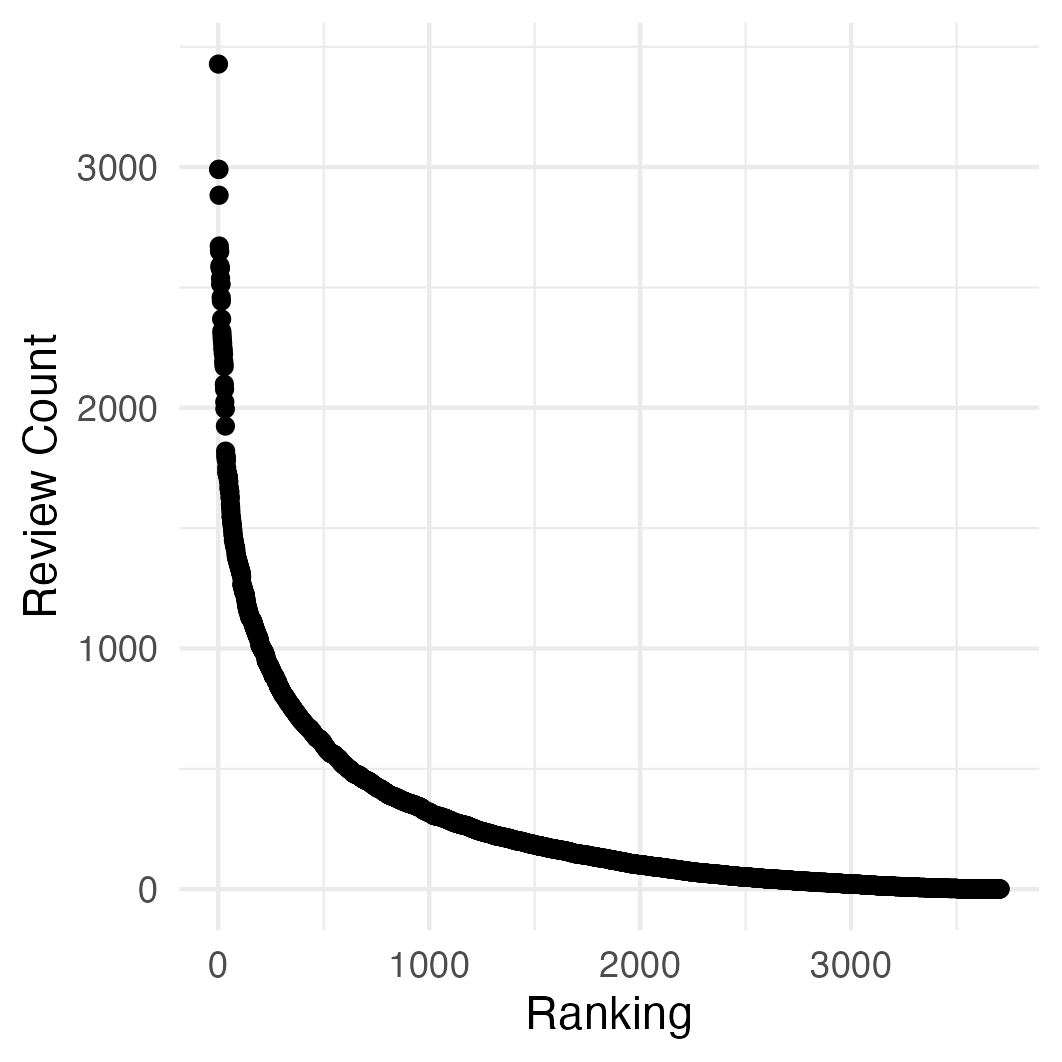
\includegraphics[width=\textwidth]{03_review_profile}
    \caption{Review profile.\label{fig:fig03_review_profile}}
  \end{subfigure}
  \begin{subfigure}{0.45\textwidth}
    \centering
    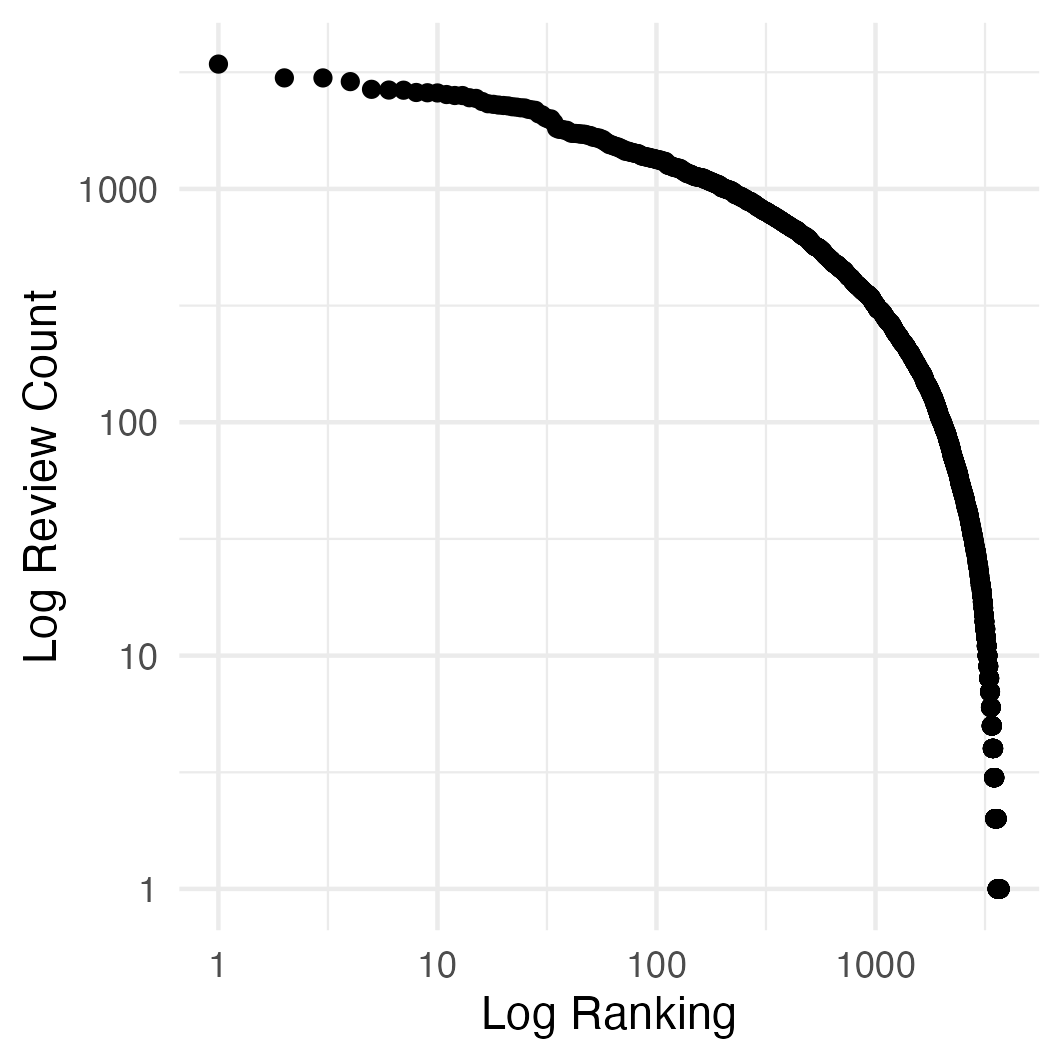
\includegraphics[width=\textwidth]{03_log_review_profile}
    \caption{Log-log plot.\label{fig:fig03_log_review_profile}}
  \end{subfigure}
  \caption{Review profile for the full dataset (a) and log-log
  plot (b).\label{fig:fig03_review_profile_both}}
\end{figure}

\subsection{Trivial Model}
\label{subsec:trivial}

Its recommendation profile can be seen in Figure~\ref{fig:fig1} and, since it is
the sum of many uniform samples, the number of times each movie is recommended
approaches a normal distribution and, therefore, the recommendation profile also
approaches the cumulative distribution function (CDF) of said distribution. The
most recommended movie appeared 25 times in the final list, while the least
recommended movie did not appear at all. Figure~\ref{fig:fig1b} shows the
log-log plot of the recommendation profile.

\begin{figure}
  \centering
  \begin{subfigure}{0.45\textwidth}
    \centering
    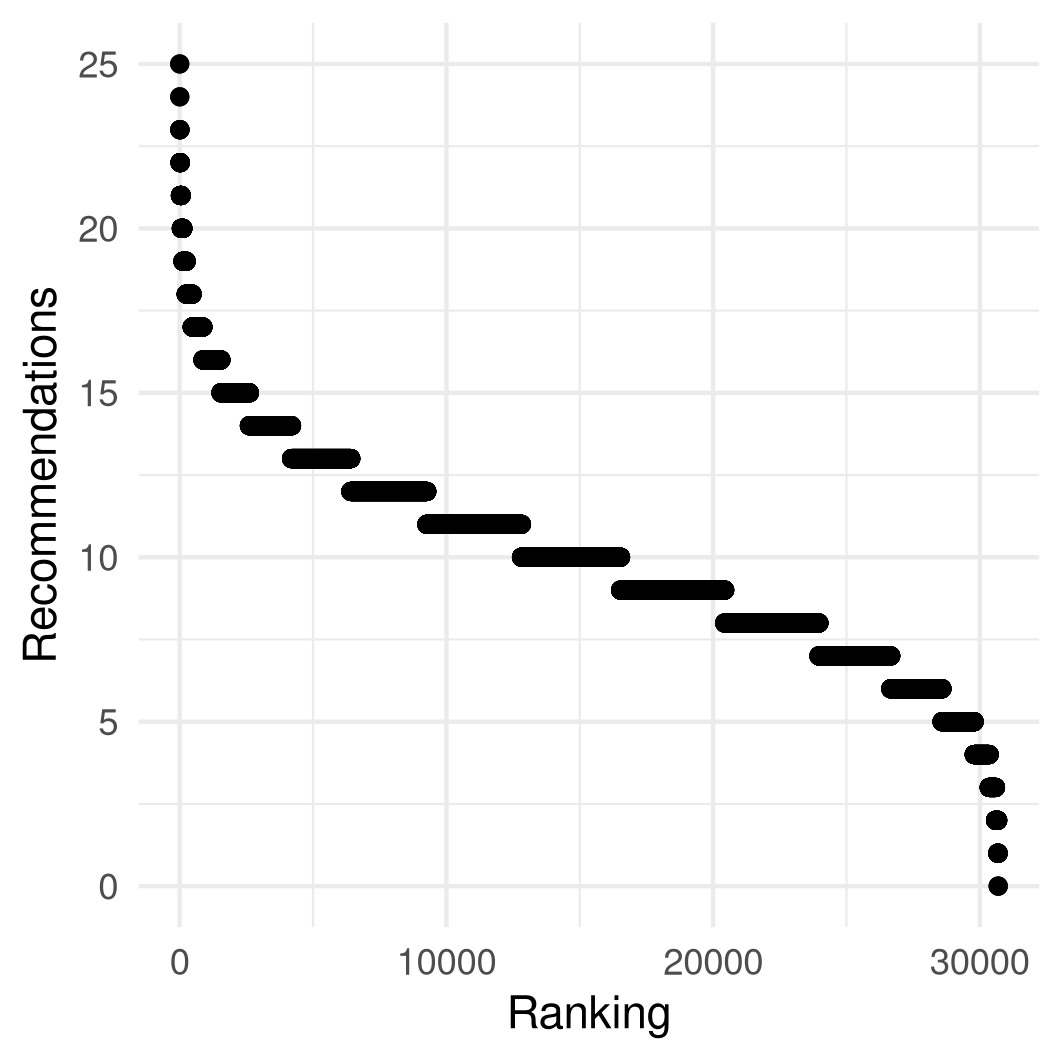
\includegraphics[width=\textwidth]{1a_random}
    \caption{Recommendation profile.\label{fig:fig1a}}
  \end{subfigure}
  \begin{subfigure}{0.45\textwidth}
    \centering
    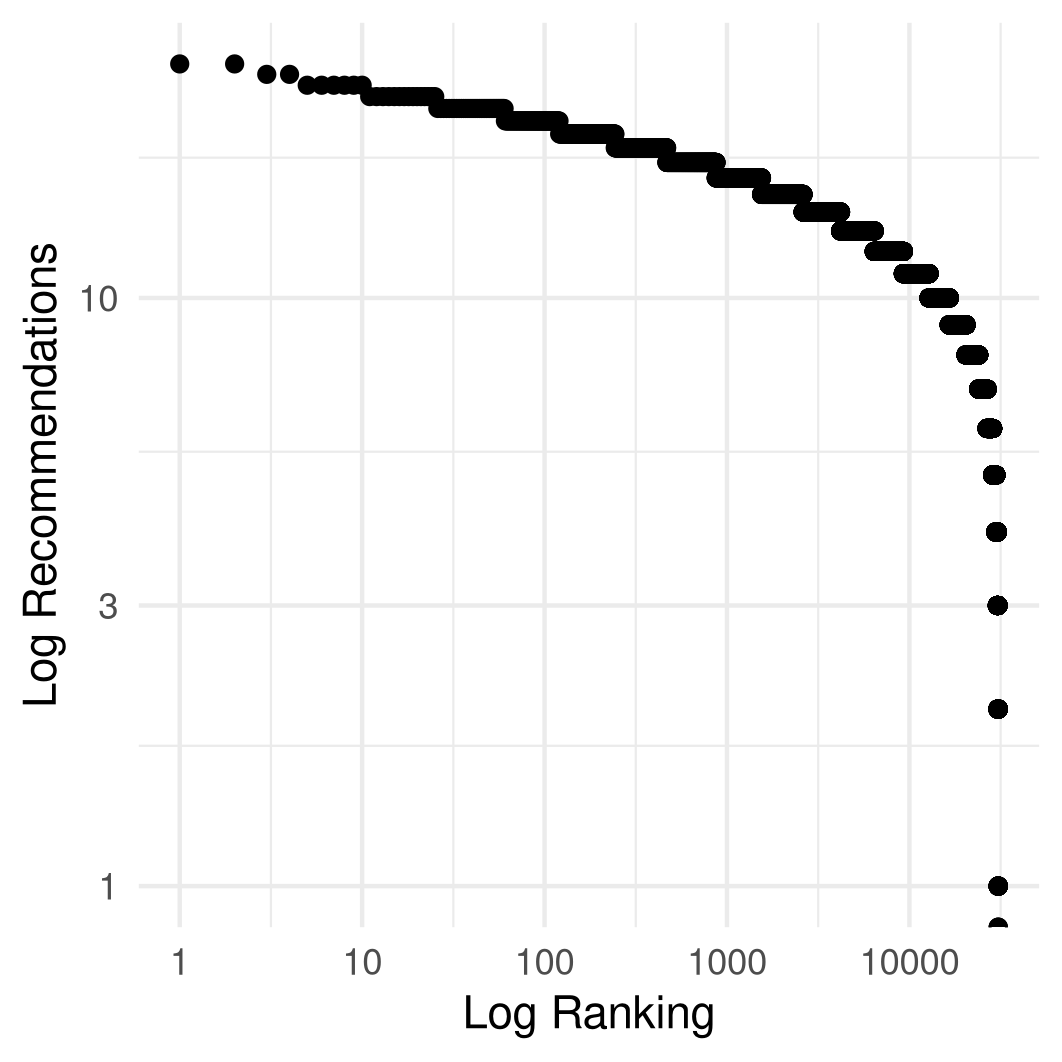
\includegraphics[width=\textwidth]{1b_random_log}
    \caption{Log-log plot.\label{fig:fig1b}}
  \end{subfigure}
  \caption{Recommendation profile for the trivial model (a) and log-log plot
    (b).\label{fig:fig1}}
\end{figure}

\subsection{Vanilla Model}
\label{subsec:vanilla}

The recommendation profile for the vanilla model can be seen in
Figure~\ref{fig:fig2a}. Here, the movie ranked number 1 appeared more than 2000
times in the full list of recommendations, with a power law decay in the number
of appearances from then on, as made evident by the log-log plot on
Figure~\ref{fig:fig2b}. This recommendation profile is a big departure from the
trivial model discussed above.

\begin{figure}
  \centering
  \begin{subfigure}{0.45\textwidth}
    \centering
    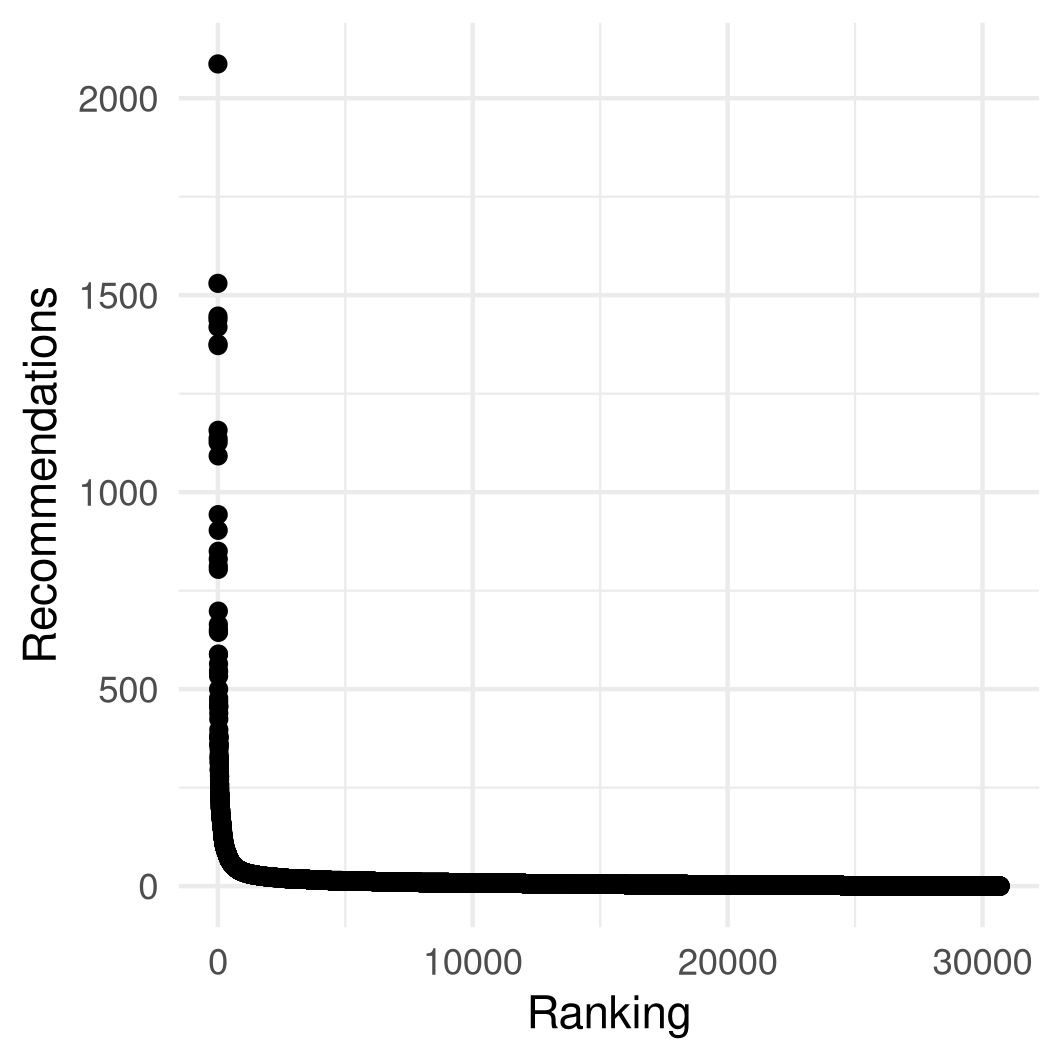
\includegraphics[width=\textwidth]{2a_vanilla}
    \caption{Recommendation profile.\label{fig:fig2a}}
  \end{subfigure}
  \begin{subfigure}{0.45\textwidth}
    \centering
    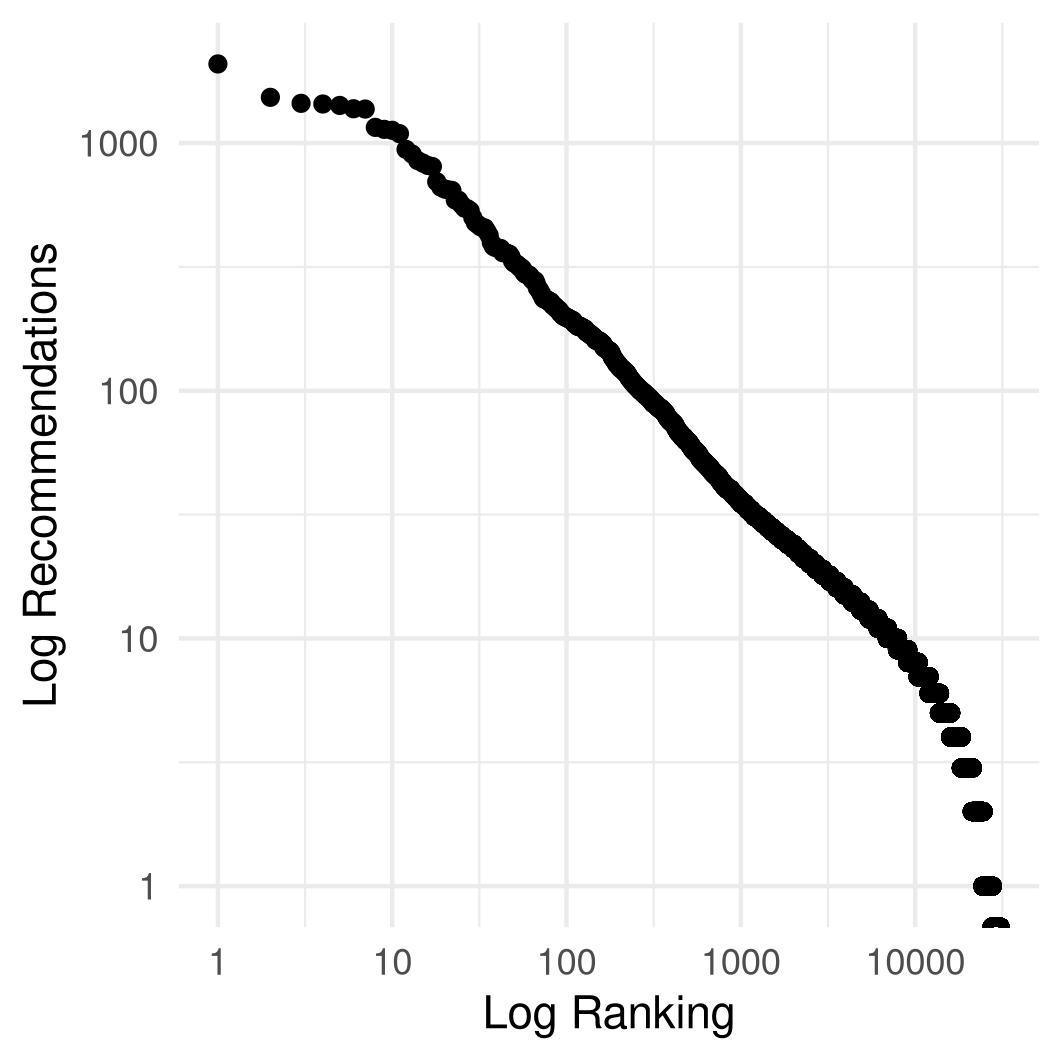
\includegraphics[width=\textwidth]{2b_vanilla_log}
    \caption{Log-log plot.\label{fig:fig2b}}
  \end{subfigure}
  \caption{Recommendation profile for the vanilla model (a) and log-log plot
    (b).\label{fig:fig2}}
\end{figure}

\subsection{Cutoff Models}
\label{subsec:cutoff}

A potential explanation for the difference between trivial and vanilla could
reside in the least used terms in the metadata and that is why we developed the
cutoff model. The results can be seen in Figure~\ref{fig:fig3} and, aside from
variations in the $y$-intercept, all plots are qualitatively very similar to
Figure~\ref{fig:fig2a}, indicating that rare words probably are not to blame for
the power law decay.

\begin{figure}
  \centering
  \begin{subfigure}{0.3\textwidth}
    \centering
    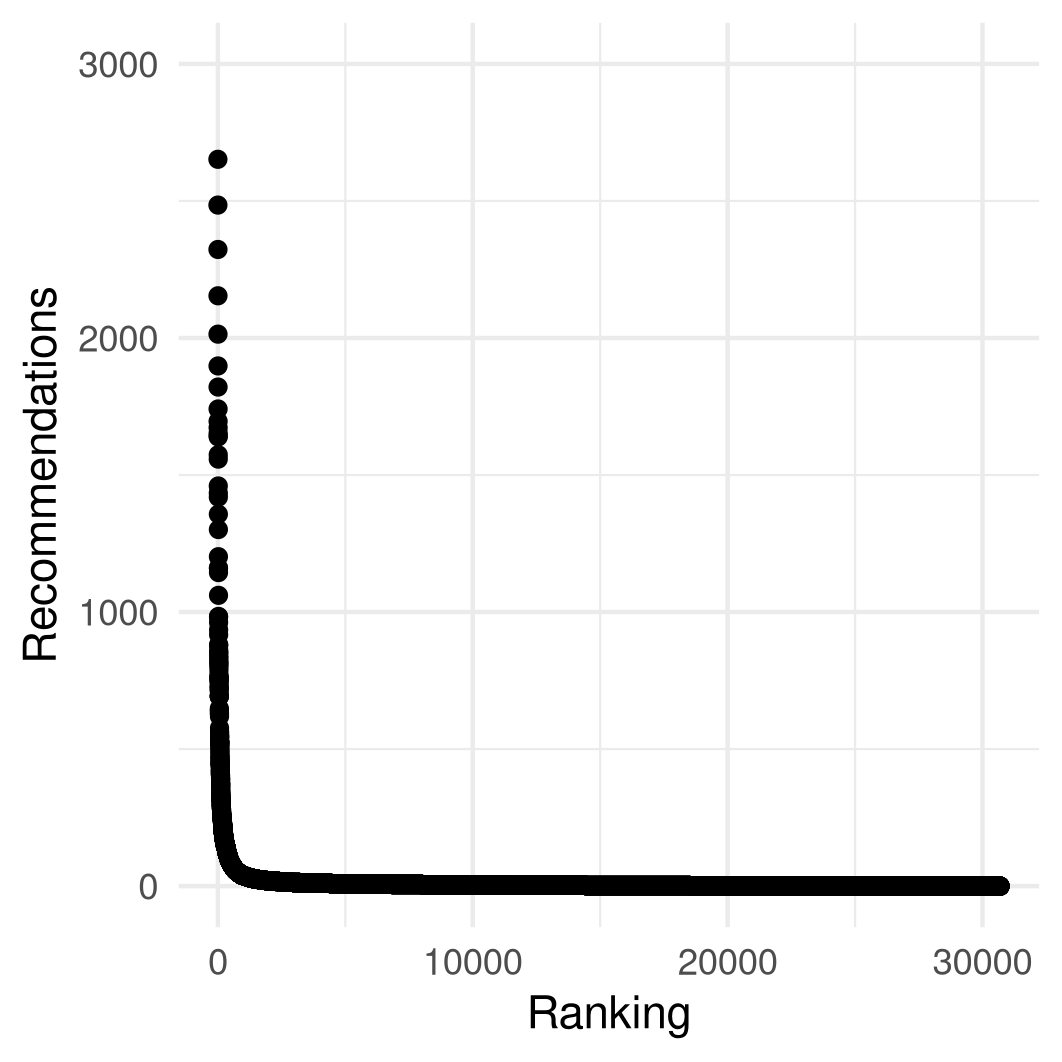
\includegraphics[width=\textwidth]{3a_cutoff_low}
    \caption{Cutoff $k = 2$.\label{fig:fig3a}}
  \end{subfigure}
  \begin{subfigure}{0.3\textwidth}
    \centering
    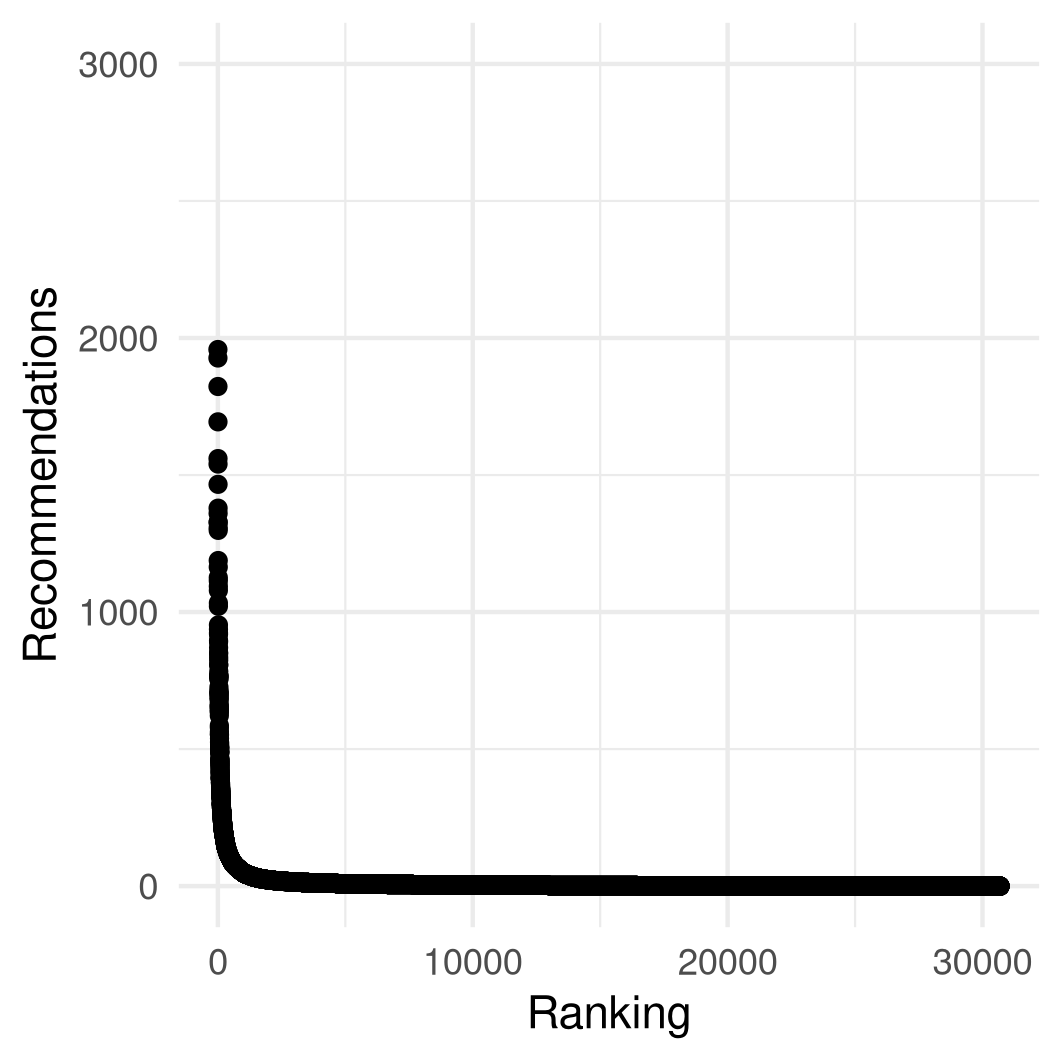
\includegraphics[width=\textwidth]{3b_cutoff_med}
    \caption{Cutoff $k = 5$.\label{fig:fig3b}}
  \end{subfigure}
  \begin{subfigure}{0.3\textwidth}
    \centering
    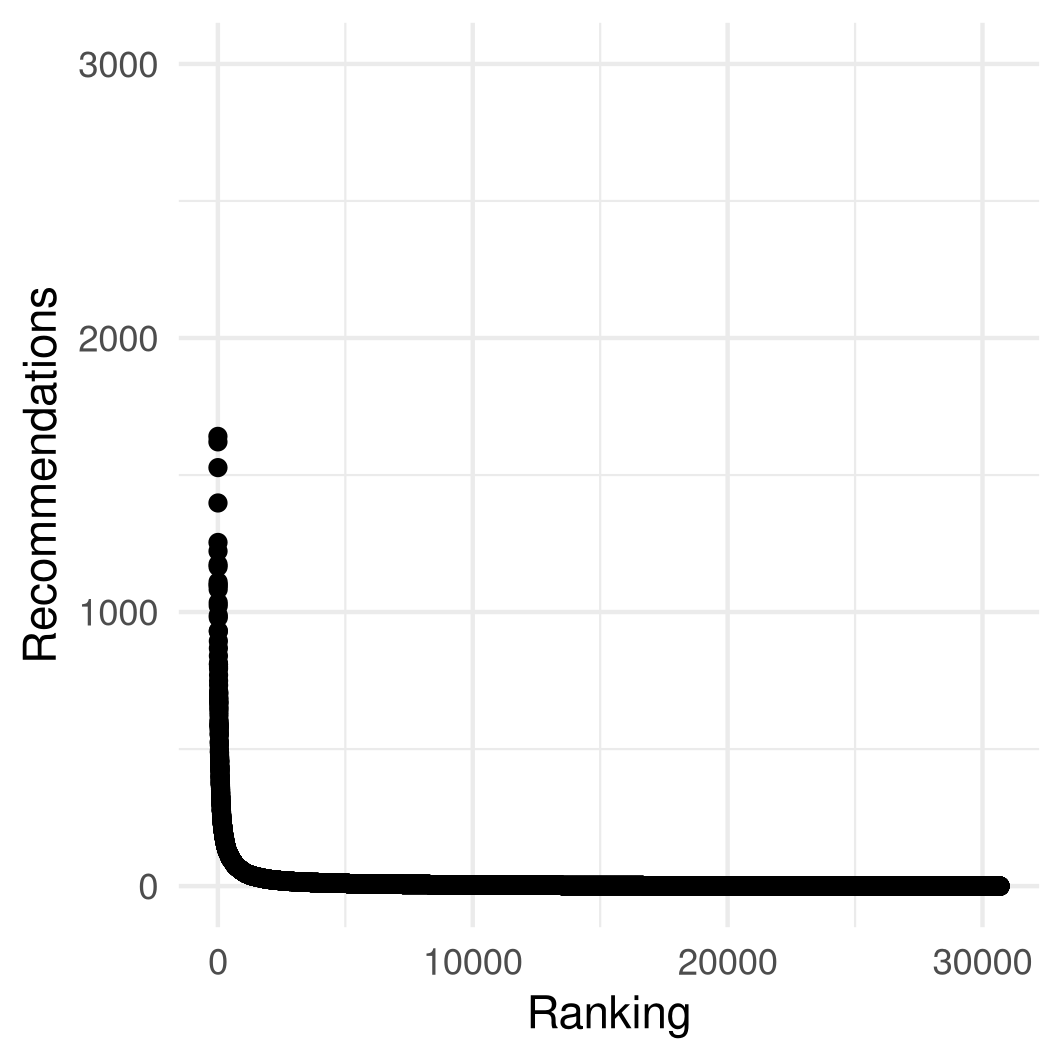
\includegraphics[width=\textwidth]{3c_cutoff_high}
    \caption{Cutoff $k = 8$.\label{fig:fig3c}}
  \end{subfigure}
  \caption{Recommendation profile for cutoff $k = 2$ (a), $5$ (b), and $8$
    (c).\label{fig:fig3}}
\end{figure}

\subsection{Similarity Models}
\label{subsec:similarity}

Since the similarity metric could also be a source of the strange behavior of
the recommendation profile, we conceived the three similarity models described
in the last section. Figure~\ref{fig:fig4} showcases a comparison between cosine
distance, euclidean distance and manhattan distance. It is clear that there are
no meaningful differences between the recommendation profiles generated by each
metric.

\begin{figure}
  \centering
  \begin{subfigure}{0.3\textwidth}
    \centering
    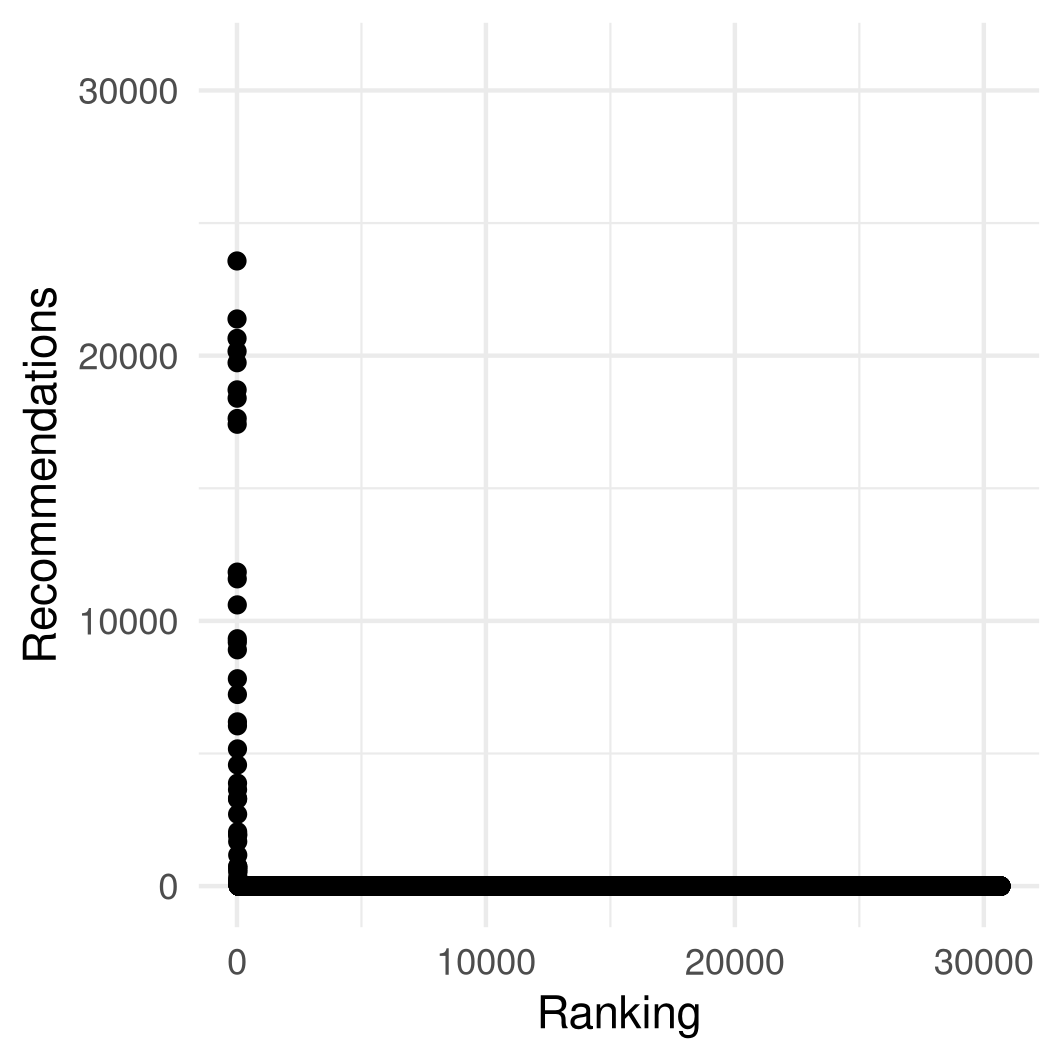
\includegraphics[width=\textwidth]{4a_cosine}
    \caption{Cosine distance (vanilla).\label{fig:fig4a}}
  \end{subfigure}
  \begin{subfigure}{0.3\textwidth}
    \centering
    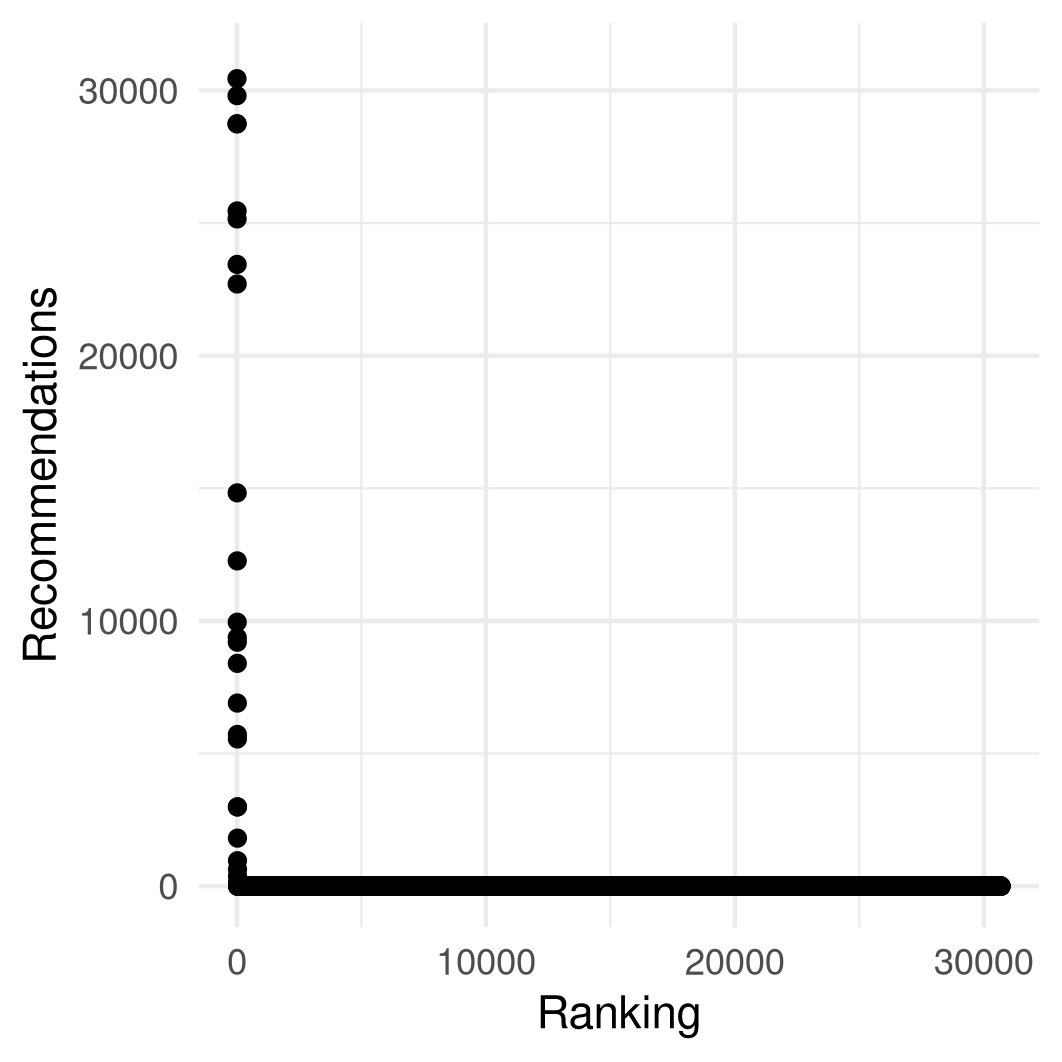
\includegraphics[width=\textwidth]{4b_euclidean}
    \caption{Euclidean distance.\label{fig:fig4b}}
  \end{subfigure}
  \begin{subfigure}{0.3\textwidth}
    \centering
    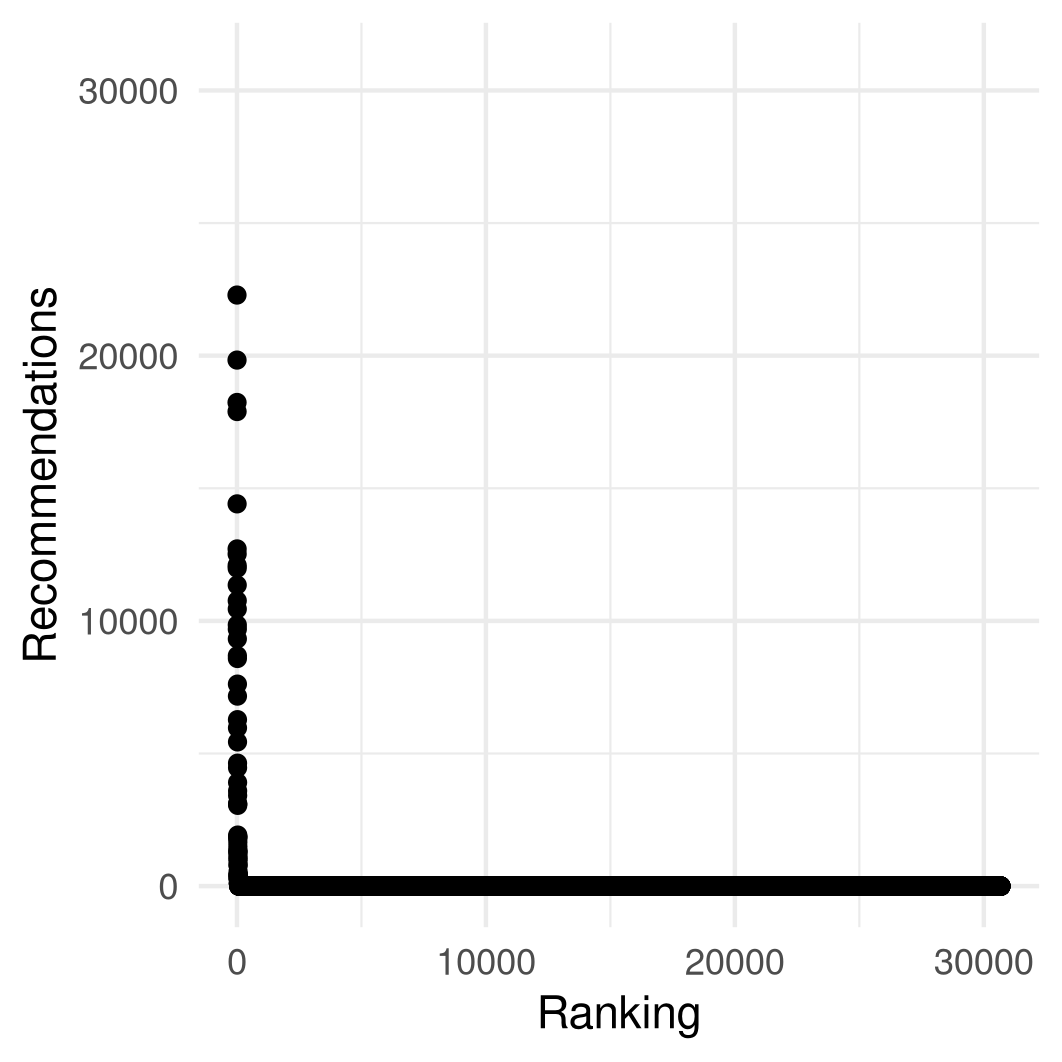
\includegraphics[width=\textwidth]{4c_manhattan}
    \caption{Manhattan distance.\label{fig:fig4c}}
  \end{subfigure}
  \caption{Recommendation profile for cosine (a), euclidean (b), and manhattan
    (c) distances.\label{fig:fig4}}
\end{figure}

\subsection{Vanilla Model with Synthetic Metadata}
\label{subsec:synthetic}

At this point it is safe to say that the type of decay seen in recommendation
frequencies up until now is not spurious and must have a clear cause. To better
investigate whether word frequency had an impact on the recommendation profiles
another hypothesis was taken into consideration: do metadata with less words
cause the recommendation curves to display a steep left-hand side?

Figure~\ref{fig:fig5} displays the recommendation profiles for the vanilla model
applied to datasets with synthetic metadata. Concretely, the figures are
equivalent to creating random metadata for the movies where the probability of
any single word being selected was approximately $1.54 \times 10^{-4}$, $1.54
\times 10^{-3}$, and $1.54 \times 10^{-2}$ respectively. The results do support
the aforementioned hypothesis since denser vectors indeed affected the decay.

\begin{figure}
  \centering
  \begin{subfigure}{0.3\textwidth}
    \centering
    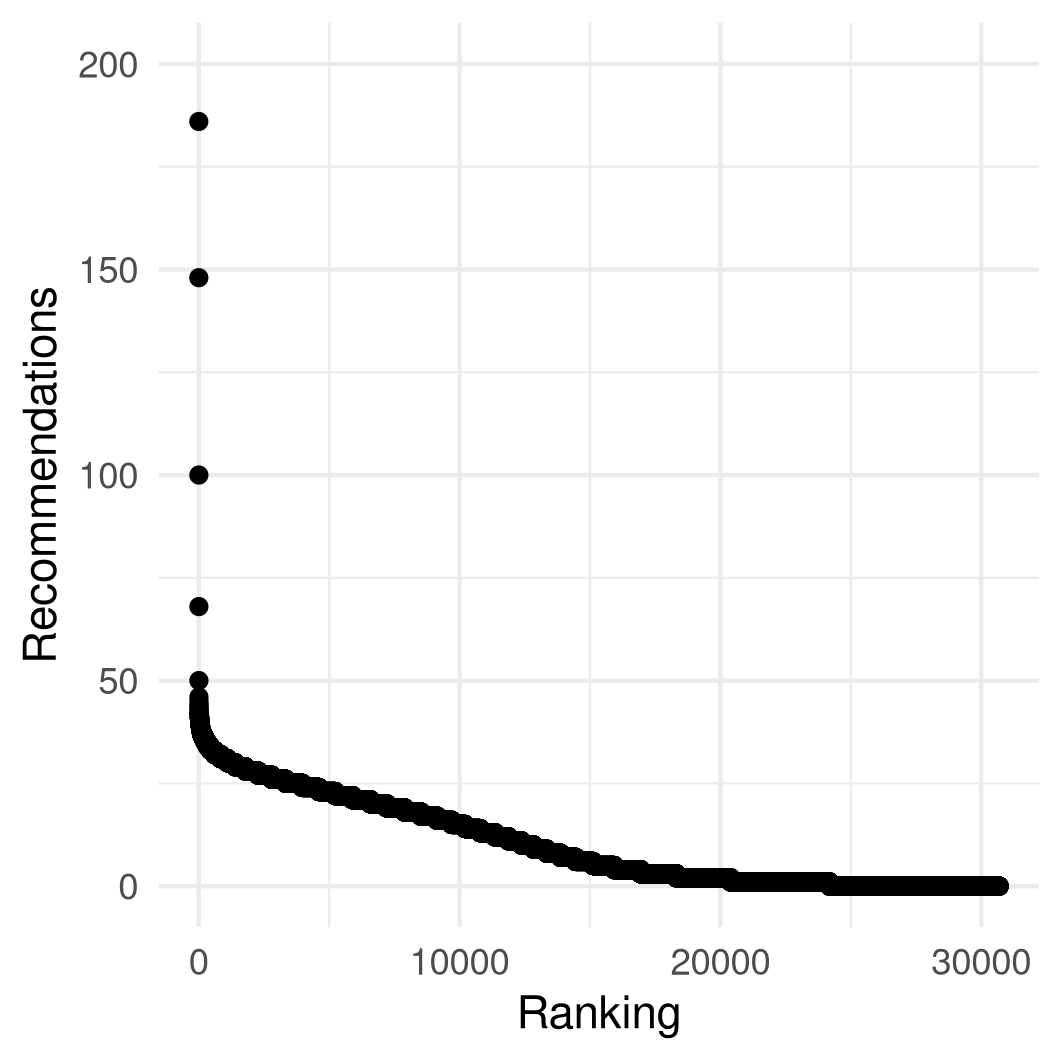
\includegraphics[width=\textwidth]{5a_p}
    \caption{$P(w_{i}) = 1 \times \overline{P(w)}$.\label{fig:fig5a}}
  \end{subfigure}
  \begin{subfigure}{0.3\textwidth}
    \centering
    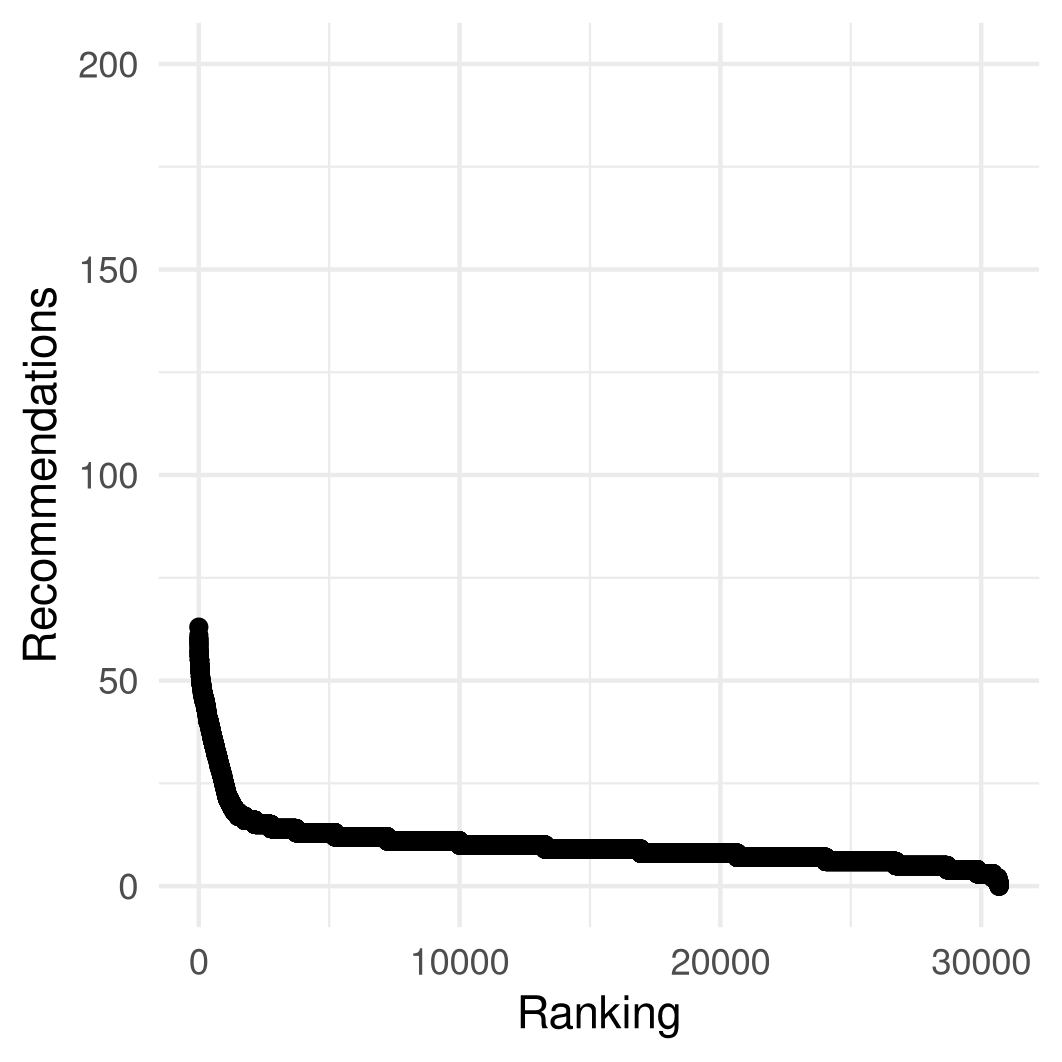
\includegraphics[width=\textwidth]{5b_p10}
    \caption{$P(w_{i}) = 10 \times \overline{P(w)}$.\label{fig:fig5b}}
  \end{subfigure}
  \begin{subfigure}{0.3\textwidth}
    \centering
    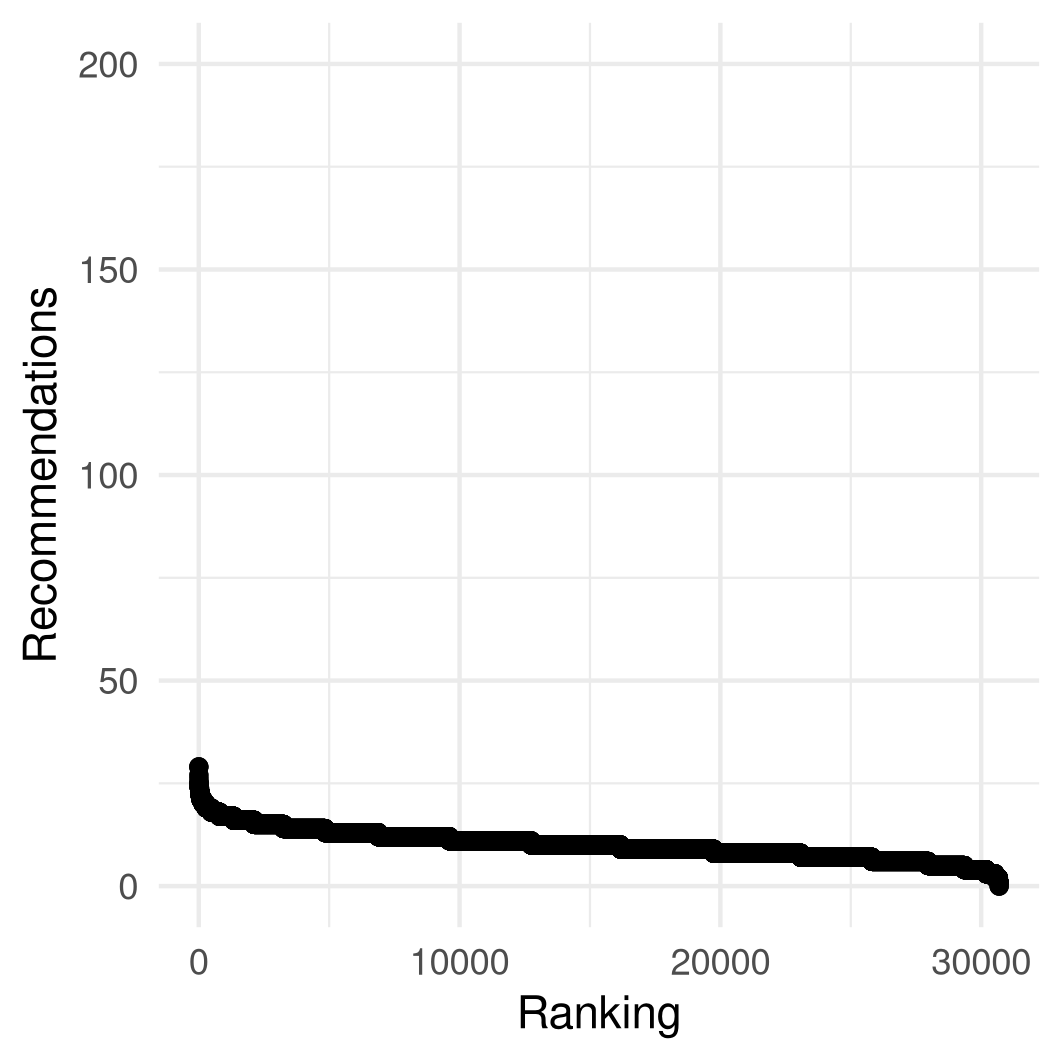
\includegraphics[width=\textwidth]{5c_p100}
    \caption{$P(w_{i}) = 100 \times \overline{P(w)}$.\label{fig:fig5c}}
  \end{subfigure}
  \caption{Recommendation profile of samples with
    $P(w_{i}) = C \times \overline{P(w)}$, $C = 1$ (a), $10$ (b), and $100$
    (c).\label{fig:fig5}}
\end{figure}

\subsection{Sanity Checks}
\label{subsec:sanity03}

After the previous experiments, sanity checks were needed in order to verify
that our previous results weren't spurious. The first check should check whether
an artificial movie created as a combination of the metadata from other movies
favored by the recommendation algorithm would also be favored (i.e. we are able
to create a popular movie from other popular movies), while the second should
check whether shorter vectors would change the decay already observed despite
being as sparse as their longer counterparts (i.e. the intrinsic properties of
the dataset aren't responsible for the power law decay). We repeated these tests
thousands of times and the results presented below are typical of what we found.

Figure~\ref{fig:fig6} showcases the two sanity checks. Figure~\ref{fig:fig6a}
was a model applied to the vanilla dataset with the addition of the movie
highlighted in red. As expected, this movie also showed up in the
top-recommended subset. Figure~\ref{fig:fig6b} comes from a model applied to
randomly generated vector representations in a similar fashion to the ones in
Figure~\ref{fig:fig5}, except each vector could only have 15,000 elements
instead of 55,681 (as with the vanilla model).

\begin{figure}
  \centering
  \begin{subfigure}{0.45\textwidth}
    \centering
    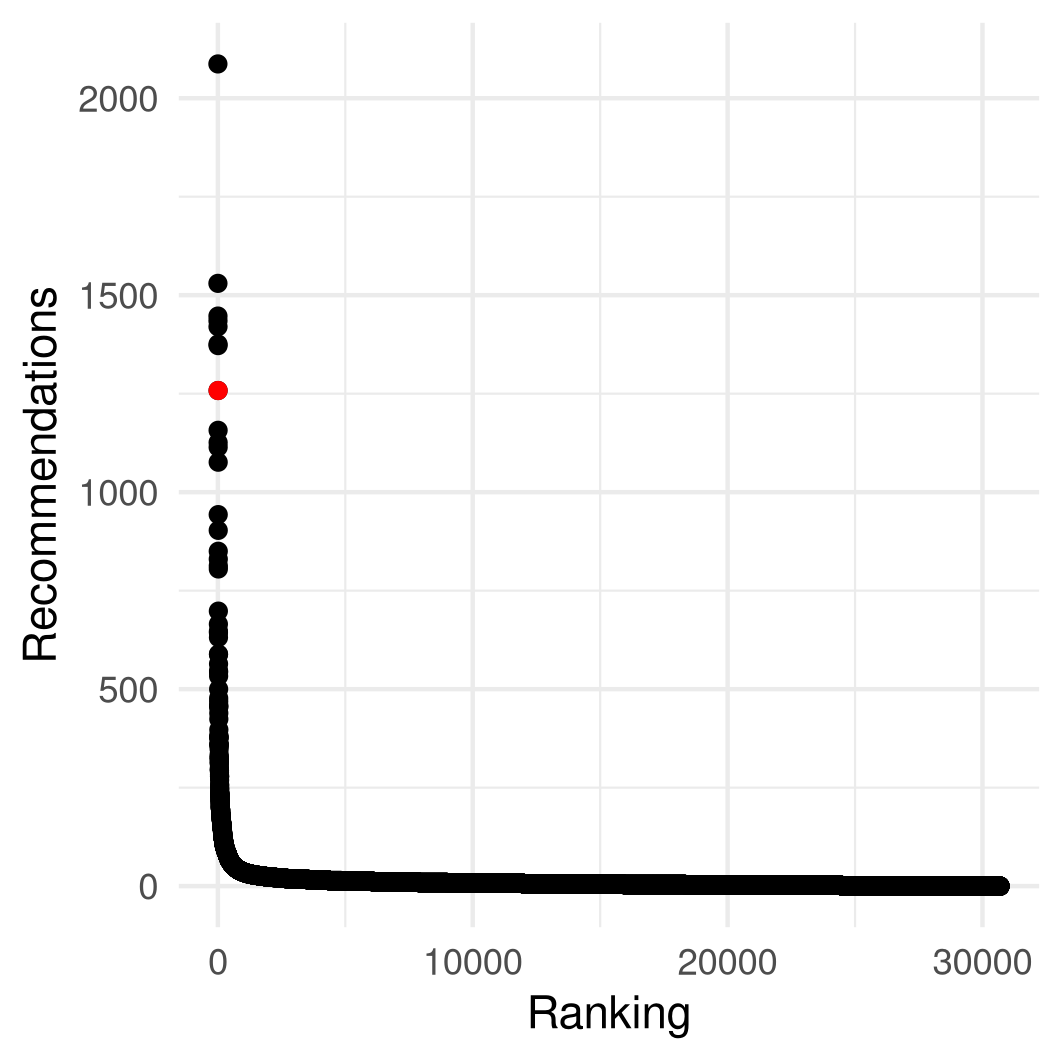
\includegraphics[width=\textwidth]{6a_artificial_movie}
    \caption{Vanilla model with artificial movie in red.\label{fig:fig6a}}
  \end{subfigure}
  \begin{subfigure}{0.45\textwidth}
    \centering
    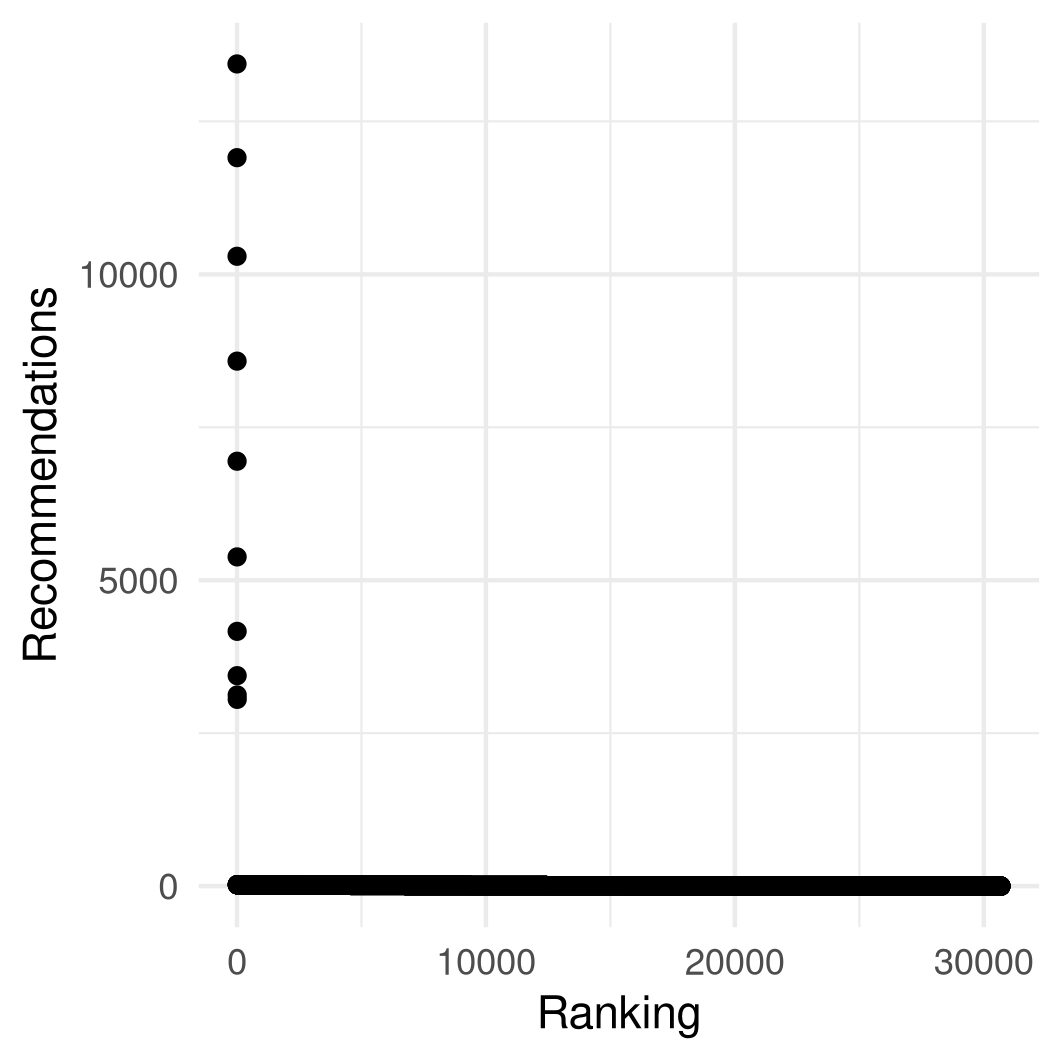
\includegraphics[width=\textwidth]{6b_long}
    \caption{Model with short vector representations.\label{fig:fig6b}}
  \end{subfigure}
  \caption{Recommendation profile for artificial movie (a) and short vector
    representations (b).\label{fig:fig6}}
\end{figure}

The last two models were considered the confirmations of the hypothesis that (at
least for this kind of recommendation systems) a subset of items was always much
more recommended than the rest as long as the data was sparse.
Figure~\ref{fig:fig7a} represents the same recommendation algorithm applied to
another dataset, the Book-Crossing dataset. Figure~\ref{fig:fig7b} contains the
results of the model applied to another set of random vector representations,
this time with the probability of each element being non-zero respecting the
marginal distributions of the vanilla dataset. Again, the power law decay
pattern persisted, only slightly less pronounced in the Book-Crossing case.

\begin{figure}
  \centering
  \begin{subfigure}{0.45\textwidth}
    \centering
    \includegraphics[width=\textwidth]{7a_books}
    \caption{Recommendation profile for book dataset.\label{fig:fig7a}}
  \end{subfigure}
  \begin{subfigure}{0.45\textwidth}
    \centering
    \includegraphics[width=\textwidth]{7b_mimic}
    \caption{Random simularion of vanilla.\label{fig:fig7b}}
  \end{subfigure}
  \caption{Recommendation profile for book dataset (a) and random simulation of
    vanilla (b).\label{fig:fig7}}
\end{figure}

The analysis up until now has been static, that is, the recommendation model
does not learn from the users' responses to its suggestions. There is no
interaction with users and no opportunity to evolve over time. The next chapter
addresses this point by using Google's newly released TensorFlow Recommenders
library \citep{noauthor_tensorflow_nodate} to gather data about what happens to
a system's recommendations as users follow its suggestions. Employing a deep
learning model that is able to improve over time is a significant departure from
the content-based models presented here and, if a similar recommendation profile
can also be detected for multi-criteria recommender systems on dynamic
scenarios, then the hypothesis ventilated in the section above would become even
more plausible.

\par

%!TeX root=../tese.tex
%("dica" para o editor de texto: este arquivo é parte de um documento maior)
% para saber mais: https://tex.stackexchange.com/q/78101/183146

\chapter{Dynamic Analysis}
\label{cap:dynamic}

Following the static analysis, it became clear that a dynamic analysis would be
of the utmost importance. Understanding how the recommendation model responds to
users reinforcing its internal biases, like the ones already detected, could
potentially lead to a better understanding of how these systems favor certain
kinds of content.

In order for this analysis to be more true to reality, we implemented a simple
recommendation algorithm using TensorFlow Recommenders \citep{}, a library for
machine learning developed by Google for use with its TensorFlow \citep{}
framework. This means that, even though our model is deliberately bare-bones, it
conforms to industry-standard technology and practices.

The choice to use a simple recommendation algorithm instead of a more complex
one was twofold: first, we didn't want to use a model that could introduce many
confounding parameters to the analysis (e.g. hyperparameters, hardware
requirements, etc.), and second, we wanted to study a baseline that could, in
the future, be used as a comparison point for more complex algorithms.

The goal of this analysis is to gather data on how the recommendation system
behaves over time. As will be explained in the next sections, is to understand
what happens to the recommendation profile of the algorithm as it interacts with
itself via users that follow the generated suggestions.

The expectation is that the recommendation profile will grow ever more steep,
which is a reasonable guess; if the users reinforce the beliefs of the
algorithm, then is stands to reason that it will recommend popular movies with
more and more frequently, to more and more users. How much more frequently,
however, is the true question.

For the sake of clarity, let's imagine two users with very distinct preferences:
Alice, who enjoys adventure movies, and Bob, who enjoys horror movies. In
principle, the algorithm should have very different recommendations for both of
them and, were they to follow them, their custom suggestions should grow
increasingly different. At the end of this experiment, users like Alice would
all be recommended the same movies, and users like Bob would have their own set
of very popular films; we should expect, therefore, a multimodal distribution of
the recommendation frequencies, with "typical" adventure movies and "typical"
horror movies being much more popular than comedy, for example.

However, if the final recommendation profile looked like what was showcased in
the previous chapter, i.e. a very small subset of movies being recommended to
most users, then we could infer that the system devolved into a degenerate
feedback loop, ignoring personal preferences and distinctions between films.

\section{Datasets}
\label{sec:datasets04}

For the dynamic experiments, we kept using the Movielens dataset \citep{}. This
time, however, we used the full ``1M'' dataset instead of sampling movies from
the larger ``25M'' version. Given that we wanted our dynamic analysis to be
conducted in a realistic scenario, we decided that it would be better not to
change the data. This whole experiment will, therefore, use a version of the
dataset commonly used for machine learning benchmarks with no alteration
whatsoever.

The 1M dataset contains 1,000,209 ratings of almost 4000 movies made by over
6000 anonymous MovieLens users who joined the platform in 2000. In this
particular version, each user has made at least 20 ratings. There are 4 columns
available:

\begin{itemize}
  \item \verb|UserID|: Unique user identifier, ranging from 1 to 6040.
  \item \verb|MovieID|: Unique movie identifier, ranging from 1 to 3952.
  \item \verb|Rating|: Movie rating according to user, from 0 to 5 stars.
  \item \verb|Timestamp|: When the user made the rating, in seconds since the
  epoch.
\end{itemize}

A second, auxiliary, dataset was also used to enrich the main one. ``Movies''
contains extra information about the movies in 1M, which allowed us to add more
variables to the recommendation system. This new dataset has 3 columns:

\begin{itemize}
  \item \verb|MovieID|: Unique user identifier, ranging from 1 to 6040.
  \item \verb|Title|: Title of the movie, as provided by IMDB.
  \item \verb|Genres|: Pipe-separated string with all applicable genres.
\end{itemize}

The other accompanying dataset, ``Users'', has not been used for the purposes of
this analysis. The reasoning behind this decision will be explained in greater
detail in the next section.

\section{Experiments}
\label{sec:experiments04}

The dynamic experiment starts in a manner much similar to the static experiment.
The full MovieLens dataset is fed as training data to a recommendation system in
order to get it ready for giving suggestions to users. As explained in the
opening section of this chapter, we chose a simple algorithm in order to reduce
the number of possible interferences architecture could have on our analysis.

The chosen recommendation algorithm was a basic ranking model described in
\citet{} using TensorFlow Recommenders \citep{}. It is composed of multiple
stacked dense layers and uses mean squared error as its loss function. The main
class in the model is reproduced below, and the full algorithm is listed in
Appendix~\ref{}.

%% Deixar o código em pseudo-código para ficar mais claro

\begin{verbatim}
class MovielensModel(tfrs.models.Model):

  def __init__(self):
    super().__init__()
    self.ranking_model: tf.keras.Model = RankingModel()
    self.task: tf.keras.layers.Layer = tfrs.tasks.Ranking(
      loss = tf.keras.losses.MeanSquaredError(),
      metrics=[tf.keras.metrics.RootMeanSquaredError()]
    )

  def call(self, features: Dict[str, tf.Tensor]) -> tf.Tensor:
    return self.ranking_model(
        (features["user_id"], features["movie_title"]))

  def compute_loss(self, features: Dict[Text, tf.Tensor],
                    training=False) -> tf.Tensor:
    labels = features.pop("user_rating")

    rating_predictions = self(features)

    # The task computes the loss and the metrics.
    return self.task(labels=labels, predictions=rating_predictions)
\end{verbatim}

In the first step of the experiment, we trained the recommendation model using
Movielens' 1M ratings dataset, which we will refer to as \verb|ratings0| from
now on. All available data was used and, in the end, we achieved a root mean
squared error (RMSE) of 0.92; this result is similar to TFRS' deep \& cross
network \citep{} results when trained on the same data. Once \verb|model0| was
ready for making recommendations, we applied it to every possible user-movie
pairing, generating a complete matrix of predicted ratings called
\verb|predictions0|.

In an environment like YouTube's recommendations sidebar, the user is presented
with a few items that the algorithm thinks they would like, and then they can
either ignore the sidebar or select one of the options to watch. Since our goal
was to explore what would happen when the recommendation system entered a
feedback loop, we picked one movie at random from each user's 10 best-ranked
entries.

This set of well-ranked movies was our way of simulating thousands of users
simultaneously approving of the algorithms recommendations and selecting one
option from their sidebars. The last step involved removing the oldest rating of
each each user from \verb|ratings0| and appending these these selections to the
dataset in order to create \verb|ratings1|. The full data flow is illustrated
in Figure~\ref{fig:fig04_dynamic_diagram}

\begin{figure}
  \centering
  \includegraphics[width=\textwidth]{04_dynamic_diagram}
  \caption{Data flow diagram.\label{fig:fig04_dynamic_diagram}}
\end{figure}

% Explicar o que são os formatos no caption da figura.

A feedback loop, however, can't be created from a single iteration. For this
reason, the process just described was classified as the ``zeroth'' iteration in
the process (as it involved \verb|ratings0|). The ``first'' iteration began with
\verb|ratings1|, trained \verb|model1|, generated \verb|predictions1|, and ended
with \verb|ratings2|. We repeated this process until we got to \verb|ratings4|,
totaling 5 ratings datasets (one original and 4 derived through ranking models).

A simplified version of the R code that created \verb|ratingsN+1| from
\verb|ratingsN| can be found below. The omitted functions served mostly
auxiliary purposes which made the datasets conform to TensorFlow's format
expectations. The full code is listed in Appendix~\ref{}.

\begin{verbatim}
predictions |>
  group_by(user_id) |>
  slice_max(prediction, n = 10) |>
  slice_sample(n = 1) |>
  ungroup() |>
  bind_rows(old_ratings) |>
  group_by(user_id) |>
  slice_max(timestamp, n = -1, with_ties = FALSE) |>
  ungroup()
\end{verbatim}

With these new datasets we were able to analyze the differences between distinct
generations of models and understand exactly how the positive feedback loop
influenced the last iteration.

A series of analysis were conducted using these datasets as sources. We found
that, with each iteration, the recommendation profile got steeper and steeper,
that is, a few popular items got more recommended while the rest fell into
disfavor; this was predictably more noticeable in movies with higher average
ratings. In fact, a small set of around 20 movies were the only ones that
consistently rose in popularity with new iterations.

Figure~\ref{fig:fig04_profile_grouped} has five subplots which represent each
iteration of the recommendation system. For \verb|ratings0|, it's possible to
see that a number of well-rated movies were more popular, i.e., were rated by
more people. Once we generate the first batch of recommendations, we add up the
number of users each movie was recommended to; this is seen in the second plot,
\verb|ratings1|. We can clearly see that a small subset of movies strayed from
the pack and to more people that had watched them previously.

This process repeats itself until, in \verb|ratings4|, the most popular movie is
recommended more than 2000 times, while the most popular movie in
\verb|ratings0| was watched a little over 500 times.

As explained before, we expected that movies which where already popular would
be recommended more times, but these plots indicate a powerful feedback loop.
Examining the data, we saw that the algorithm was consistently recommending
movies which the users had already watched and this process only became more
accentuated with each subsequent iteration.

\begin{figure}
  \centering
  \includegraphics[width=\textwidth]{04_profile_grouped}
  \caption{Recommendation profile of every generation. Colors indicate average
  movie rating, which is a strong predictor of popularity over time.
  \label{fig:fig04_profile_grouped}}
\end{figure}

% explicar que, nos gráficos, popularidade significa número de recs para t = 1..4

A good way to measure how diverse were the recommendations made by the algorithm
is to calculate the entropy \citep{} of each set. In the extreme, if the same
movie is recommended to every user, than the entropy of the recommendations will
tend to zero. In absolute terms, the entropy of \verb|ratings0| was 7.42, and
the entropy of \verb|ratings4| was 6.08 (82\% lower). A comparison in relative
terms is displayed in Figure~\ref{fig:fig04_entropy}.

\begin{figure}
  \centering
  \begin{subfigure}{0.45\textwidth}
    \centering
    \includegraphics[width=\textwidth]{04_entropy}
  \end{subfigure}
  \caption{Recommendation entropy as a percentage of ratings0s entropy.
  \label{fig:fig04_entropy}}
\end{figure}

We can also observe this reduction of variety in an even more visual way. In
Figure~\ref{fig:fig04_popularity_time_both} we plotted movie popularity over
time; each line represents a movie and each step in the x-axis is a new
generation of the model. Figure~\ref{fig:fig04_popularity_time} makes it very
clear that no more than 15 movies rose in popularity over the four generations
of the recommendation system, becoming orders of magnitude more popular than the
rest. We also scaled the y-axis by taking the its log in
Figure~\ref{fig:fig04_log_popularity_time}, and we can see that, in fact, no
other movie rose in popularity besides the ones that stick out after
\verb|model2|.

It is also of note that the few movies that rise in popularity are not the most
popular ones from \verb|ratings0|, even though genre was the only metadata we
fed into the system. This uncovers a significant feature of the feedback loop we
observed in Figure~\ref{fig:fig04_profile_grouped}: the items that the algorithm
amplifies don't necessarily have to be the most mainstream, or in other words,
recommendation systems are able to boost content artificially.

\begin{figure}
  \centering
  \begin{subfigure}{0.45\textwidth}
    \centering
    \includegraphics[width=\textwidth]{04_popularity_time}
    \caption{Movie popularity over time.\label{fig:fig04_popularity_time}}
  \end{subfigure}
  \begin{subfigure}{0.45\textwidth}
    \centering
    \includegraphics[width=\textwidth]{04_log_popularity_time}
    \caption{Movie log-popularity over time.\label{fig:fig04_log_popularity_time}}
  \end{subfigure}
  \caption{Popularity of every movie from ratings0 to ratings4.\label{fig:fig04_popularity_time_both}}
\end{figure}

\section{Modeling}
\label{sec:modeling04}

Having identified a feedback loop in the recommendation system, we decided to
fit a regression model on our generated data. The goal of this step is
essentially explainability \citep{}: to help better understand the algorithms
decisions.

% Computational Statistics do James E. Gentle

As is common in computational inference \citep{}, our process involved multiple
rounds of modeling. We started with a very simple model and, according to
goodness-of-fit measurements, made it more and more complex in order to achieve
a better representation of the behavior of the recommendation system. As we will
see later, even after feeding all of the the available data (and some extra
metadata that the recommender algorithm didn't have access to), our models were
not able to capture such a degenerate distribution.

The first model we attempted to use was a simple Poisson regression \citep{}.
Since the recommendation profiles displayed a strong positive skew and an
exponential-like decay, a log-linear model seemed like a good starting point.
For this kind of model \citep{}, we take a set of $\mathbf{x} \in
\mathbb{R}^{n}$ and fit a regression of the form

$$
\log(\operatorname{E} (Y \mid \mathbf{x})) = \alpha + \mathbf{\beta}'\mathbf{x},
$$

where $\alpha \in \mathbb{R}$ and $\mathbf{\beta} \in \mathbb{R}^{n}$. More
concretely, we used R's \verb|glm()| \citep{} function with the following
formula: \verb|pop ~ t * genre * rating|. In this expression, \verb|pop|
represents the popularity of a movie, \verb|t| represents the generation i.e.
the iteration from 0 to 4, and \verb|genre| represents the genre.

As the reader might be able to see, we used the genre variable in our regression
model even though we didn't feed it to the recommendation system. As explained
before, the algorithm only had access to the popularity and ratings of the
movies, but it is possible the there exists a latent effect of genre on the
other variables; since a machine learning system is much more flexible than a
regression model, we opted to explicitly feed the genre into the Poisson model
and all others that followed.

For illustrative purposes, we will present the full output of this model below.
It is notable how many coefficients are considered highly significant, meaning
that, individually, they were able to capture the feedback loop generated by
the recommendation system.

\begin{verbatim}
Call:
glm(formula = pop ~ t * genre * rating, family = "poisson", data = features)

Deviance Residuals:
    Min       1Q   Median       3Q      Max
-33.145   -3.088   -1.222    1.260   93.001

Coefficients:
                            Estimate Std. Error z value Pr(>|z|)
(Intercept)                9.210e-02  9.514e-02   0.968 0.333031
t                         -6.844e-02  4.200e-02  -1.629 0.103208
genreAnimation            -2.276e+00  1.475e-01 -15.430  < 2e-16 ***
genreChildren's            1.489e-02  1.754e-01   0.085 0.932347
genreComedy               -1.904e-01  1.041e-01  -1.828 0.067539 .
genreCrime                -4.898e+00  1.858e-01 -26.364  < 2e-16 ***
genreDocumentary          -1.801e+00  4.491e-01  -4.010 6.07e-05 ***
genreDrama                -1.035e+00  1.140e-01  -9.086  < 2e-16 ***
genreFilm-Noir            -1.631e+01  5.403e-01 -30.185  < 2e-16 ***
genreHorror                3.012e-01  1.178e-01   2.556 0.010582 *
genreMusical              -2.784e+00  4.813e-01  -5.784 7.31e-09 ***
genreMystery              -4.849e+00  2.464e-01 -19.681  < 2e-16 ***
genreRomance              -1.476e+00  5.299e-01  -2.785 0.005347 **
genreSci-Fi                1.583e+00  1.898e-01   8.341  < 2e-16 ***
genreThriller              3.854e-01  1.791e-01   2.152 0.031394 *
genreWestern              -4.253e+00  5.017e-01  -8.476  < 2e-16 ***
rating                     8.877e-01  2.740e-02  32.395  < 2e-16 ***
t:genreAnimation          -3.139e+00  6.223e-02 -50.435  < 2e-16 ***
t:genreChildren's         -5.212e-04  7.760e-02  -0.007 0.994641
t:genreComedy             -2.235e-02  4.602e-02  -0.486 0.627215
t:genreCrime              -3.561e+00  8.570e-02 -41.557  < 2e-16 ***
t:genreDocumentary         2.463e-01  1.933e-01   1.274 0.202583
t:genreDrama              -1.845e+00  5.015e-02 -36.799  < 2e-16 ***
t:genreFilm-Noir          -5.419e+00  1.944e-01 -27.872  < 2e-16 ***
t:genreHorror              7.776e-03  5.217e-02   0.149 0.881511
t:genreMusical             1.190e-01  2.140e-01   0.556 0.578236
t:genreMystery            -3.676e+00  1.032e-01 -35.632  < 2e-16 ***
t:genreRomance            -8.909e-02  2.334e-01  -0.382 0.702658
t:genreSci-Fi             -2.251e+00  8.076e-02 -27.869  < 2e-16 ***
t:genreThriller            6.362e-02  7.894e-02   0.806 0.420240
t:genreWestern             5.290e-02  2.211e-01   0.239 0.810874
t:rating                  -1.584e-02  1.212e-02  -1.307 0.191193
genreAnimation:rating      7.049e-01  3.938e-02  17.900  < 2e-16 ***
genreChildren's:rating    -4.814e-02  5.303e-02  -0.908 0.364006
genreComedy:rating         1.711e-02  2.989e-02   0.572 0.567055
genreCrime:rating          1.261e+00  4.818e-02  26.161  < 2e-16 ***
genreDocumentary:rating    5.638e-02  1.160e-01   0.486 0.626776
genreDrama:rating          1.163e-01  3.199e-02   3.635 0.000278 ***
genreFilm-Noir:rating      3.865e+00  1.239e-01  31.197  < 2e-16 ***
genreHorror:rating        -1.456e-01  3.541e-02  -4.111 3.95e-05 ***
genreMusical:rating        6.395e-01  1.255e-01   5.095 3.50e-07 ***
genreMystery:rating        1.286e+00  6.114e-02  21.030  < 2e-16 ***
genreRomance:rating        3.492e-02  1.506e-01   0.232 0.816639
genreSci-Fi:rating        -5.037e-01  5.457e-02  -9.230  < 2e-16 ***
genreThriller:rating      -1.952e-01  5.094e-02  -3.833 0.000127 ***
genreWestern:rating        9.773e-01  1.309e-01   7.467 8.19e-14 ***
t:genreAnimation:rating    8.263e-01  1.631e-02  50.671  < 2e-16 ***
t:genreChildren's:rating  -1.370e-03  2.350e-02  -0.058 0.953503
t:genreComedy:rating       6.194e-03  1.323e-02   0.468 0.639610
t:genreCrime:rating        9.129e-01  2.163e-02  42.204  < 2e-16 ***
t:genreDocumentary:rating -5.843e-02  5.002e-02  -1.168 0.242813
t:genreDrama:rating        5.028e-01  1.399e-02  35.927  < 2e-16 ***
t:genreFilm-Noir:rating    1.279e+00  4.402e-02  29.061  < 2e-16 ***
t:genreHorror:rating      -6.526e-03  1.573e-02  -0.415 0.678237
t:genreMusical:rating     -3.530e-02  5.588e-02  -0.632 0.527603
t:genreMystery:rating      9.553e-01  2.495e-02  38.291  < 2e-16 ***
t:genreRomance:rating      3.023e-02  6.624e-02   0.456 0.648140
t:genreSci-Fi:rating       6.707e-01  2.195e-02  30.551  < 2e-16 ***
t:genreThriller:rating    -1.870e-02  2.252e-02  -0.830 0.406351
t:genreWestern:rating     -1.209e-02  5.768e-02  -0.210 0.834031
---
Signif. codes:  0 ‘***’ 0.001 ‘**’ 0.01 ‘*’ 0.05 ‘.’ 0.1 ‘ ’ 1

(Dispersion parameter for poisson family taken to be 1)

    Null deviance: 562028  on 13559  degrees of freedom
Residual deviance: 268737  on 13500  degrees of freedom
AIC: 318813

Number of Fisher Scoring iterations: 6
\end{verbatim}

However, analyzing the coefficients by themselves is only one part of the full
picture. We used a simulation envelope \citep{} to assess global
goodness-of-fit, which is obtained by plotting the ordered absolute values of a
model diagnostic versus the expected order statistic of a normal distribution
\citep{}:

$$
\Phi^{-1}(\frac{i+3/8}{n+1/4})
$$

% Reescrever os 2 parágrafos abaixo. Eles foram tirados direto dos docs da
% hnp::hnp()

% Atkinson (1985)
\citet{} proposed the addition of a simulated envelope, which is such that under
the correct model the plot for the observed data is likely to fall within the
envelope. The objective is not to provide a region of acceptance, but some sort
of guidance to what kind of shape to expect.

Obtaining the simulated envelope is simple and consists of (1) fitting a model;
(2) extracting model diagnostics and calculating sorted absolute values; (3)
simulating 99 (or more) response variables using the same model matrix, error
distribution and fitted parameters; (4) fitting the same model to each simulated
response variable and obtaining the same model diagnostics, again sorted
absolute values; (5) computing the desired percentiles (e.g., 2.5 and 97.5) at
each value of the expected order statistic to form the envelope.

The resulting simulated envelope was generated with the \verb|hnp| \citep{} R
package and can be seen in Figure~\ref{fig:fig04_residual_poisson}. It is plain
to see that the model does not conform to the delimited region and, therefore,
isn't able to properly capture the variability of the data.

\begin{figure}
  \centering
  \includegraphics[width=\textwidth]{04_residual_poisson}
  \caption{Residual analysis via simulated envelope for the Poisson regression.\label{fig:fig04_residual_poisson}}
\end{figure}




..., and \verb|movie_id| is the ID of a movie. Note
that the genre was not used when training the recommendation models described
above, but it turned out that this feature could explain a lot of the models'
outputs.

\begin{verbatim}
  Family: nbinom2  ( log )
Formula:          pop ~ t * genre * rating + (1 | movie_id)
Data: features

     AIC      BIC   logLik deviance df.resid
 83863.8  84370.3 -41865.9  83731.8    15844

Random effects:

Conditional model:
 Groups   Name        Variance Std.Dev.
 movie_id (Intercept) 1.364    1.168
Number of obs: 15910, groups:  movie_id, 3182

Dispersion parameter for nbinom2 family ():   49

Conditional model:
                            Estimate Std. Error z value Pr(>|z|)
(Intercept)                -0.108714   0.272464  -0.399 0.689891
t                          -0.210272   0.021153  -9.941  < 2e-16 ***
genreAdventure              0.112129   0.574197   0.195 0.845174
genreAnimation             -2.286362   0.773873  -2.954 0.003132 **
genreChildren's             0.855196   0.755919   1.131 0.257915
genreComedy                -0.108159   0.352431  -0.307 0.758925
genreCrime                 -3.590470   0.850227  -4.223 2.41e-05 ***
genreDocumentary           -1.659325   1.508329  -1.100 0.271285
genreDrama                 -1.219969   0.409312  -2.981 0.002877 **
genreFilm-Noir            -16.633103   2.371128  -7.015 2.30e-12 ***
genreHorror                 0.512807   0.443025   1.158 0.247062
genreMusical               -4.259252   2.088483  -2.039 0.041410 *
genreMystery               -4.646920   1.461852  -3.179 0.001479 **
genreRomance               -2.118789   1.856289  -1.141 0.253699
genreSci-Fi                 0.363380   1.044431   0.348 0.727899
genreThriller               1.382908   0.855392   1.617 0.105944
genreWestern               -3.766758   2.108848  -1.786 0.074072 .
rating                      0.957533   0.085468  11.203  < 2e-16 ***
t:genreAdventure            0.161327   0.053403   3.021 0.002520 **
t:genreAnimation           -0.392012   0.067698  -5.791 7.01e-09 ***
t:genreChildren's           0.116028   0.066946   1.733 0.083068 .
t:genreComedy               0.119502   0.030504   3.918 8.94e-05 ***
t:genreCrime               -0.146821   0.085503  -1.717 0.085952 .
t:genreDocumentary          0.329357   0.195776   1.682 0.092507 .
t:genreDrama                0.005393   0.038739   0.139 0.889287
t:genreFilm-Noir           -0.730742   0.227275  -3.215 0.001303 **
t:genreHorror               0.148203   0.041813   3.544 0.000393 ***
t:genreMusical              0.265118   0.243060   1.091 0.275383
t:genreMystery             -1.150785   0.123034  -9.353  < 2e-16 ***
t:genreRomance              0.064921   0.227735   0.285 0.775590
t:genreSci-Fi              -0.311108   0.079779  -3.900 9.63e-05 ***
t:genreThriller             0.134758   0.077077   1.748 0.080403 .
t:genreWestern              0.184582   0.216581   0.852 0.394073
t:rating                    0.029594   0.006273   4.717 2.39e-06 ***
genreAdventure:rating      -0.209253   0.179840  -1.164 0.244606
genreAnimation:rating       0.594327   0.226301   2.626 0.008633 **
genreChildren's:rating     -0.473591   0.247951  -1.910 0.056131 .
genreComedy:rating         -0.194909   0.109223  -1.785 0.074341 .
genreCrime:rating           0.736375   0.243050   3.030 0.002448 **
genreDocumentary:rating    -0.113489   0.399299  -0.284 0.776242
genreDrama:rating          -0.031020   0.120957  -0.256 0.797601
genreFilm-Noir:rating       3.958891   0.595316   6.650 2.93e-11 ***
genreHorror:rating         -0.422452   0.151685  -2.785 0.005352 **
genreMusical:rating         0.944897   0.569196   1.660 0.096903 .
genreMystery:rating         1.092607   0.409047   2.671 0.007560 **
genreRomance:rating         0.013712   0.548422   0.025 0.980053
genreSci-Fi:rating         -0.423339   0.324094  -1.306 0.191477
genreThriller:rating       -0.729129   0.256016  -2.848 0.004400 **
genreWestern:rating         0.725673   0.578412   1.255 0.209625
t:genreAdventure:rating    -0.053250   0.015828  -3.364 0.000768 ***
t:genreAnimation:rating     0.110189   0.018603   5.923 3.16e-09 ***
t:genreChildren's:rating   -0.039499   0.020922  -1.888 0.059031 .
t:genreComedy:rating       -0.039790   0.008913  -4.464 8.04e-06 ***
t:genreCrime:rating         0.038460   0.022654   1.698 0.089557 .
t:genreDocumentary:rating  -0.088874   0.050610  -1.756 0.079076 .
t:genreDrama:rating        -0.006800   0.010754  -0.632 0.527202
t:genreFilm-Noir:rating     0.183567   0.054187   3.388 0.000705 ***
t:genreHorror:rating       -0.052874   0.013574  -3.895 9.81e-05 ***
t:genreMusical:rating      -0.082105   0.063538  -1.292 0.196285
t:genreMystery:rating       0.335177   0.032553  10.296  < 2e-16 ***
t:genreRomance:rating      -0.018634   0.064877  -0.287 0.773939
t:genreSci-Fi:rating        0.108210   0.023442   4.616 3.91e-06 ***
t:genreThriller:rating     -0.044310   0.022584  -1.962 0.049758 *
t:genreWestern:rating      -0.055461   0.056878  -0.975 0.329521
---
Signif. codes:  0 '***' 0.001 '**' 0.01 '*' 0.05 '.' 0.1 ' ' 1
\end{verbatim}

\begin{figure}
  \centering
  \includegraphics[width=\textwidth]{04_residual_mmnb2}
  \caption{Residual analysis for glmmTMB model.\label{fig:fig04_residual_mmnb2}}
\end{figure}

\par

%!TeX root=../tese.tex
%("dica" para o editor de texto: este arquivo é parte de um documento maior)
% para saber mais: https://tex.stackexchange.com/q/78101/183146

\chapter{Conclusion}
\label{cap:conclusion}

In this work, we studied recommender system bias. As detailed in
Chapter~\ref{cap:introduction}, these algorithms are pervasive in modern live
and have significant impact on our information diet; however, a growing body of
evidence indicates that these systems, specially when deployed in large social
networks, can display significant biases in their recommendations. Researchers
and activists alike worry that these biases might create echo chambers and
radicalization pipelines by amplifying extremist content. In broad terms, our
goal was to study one way through which these algorithms might be boosting
fringe viewpoints and radicalizing users: degenerate feedback loops.

Degeneracy in recommender systems has been explored before by
\citet{nguyen_exploring_2014} and \citet{jiang_degenerate_2019}. They concluded
that these algorithms show a tendency to reduce the diversity of recommended
content over time because of the feedback loop that occurs when the system must
learn from the its own outputs. Our main research objective was to further
characterize and model this behavior using both qualitative and quantitative
methods.

In Chapter~\ref{cap:review}, we reviewed the scientific literature that deals
with this topic and presented a few different viewpoints on the matter. Works by
\citet{hosseinmardi_evaluating_2020}, \citet{huszar_algorithmic_2021}, and
others suggest that social networks tend to amplify far-right views, while
\citet{munger_right-wing_2020} and \citet{ledwich_algorithmic_2019} posit that
this is not the case. \citet{ribeiro_auditing_2020} found evidence that, in
general, YouTube users tend to migrate from "lighter" content towards more
extreme videos, and \citet{stoica_algorithmic_2018} coined the term
``algorithmic glass ceiling'' to describe recommender system's propensity to
reinforce homophilic behavior.

We also drew attention to non-scientific endeavors that attempt to better
understand filter bubbles, echo chambers, and their impacts on the public. While
this issue is being debated in academia, journalists and whistleblowers like
\citet{ribeiro_como_2021} or \citet{wong_how_2021} hold social media companies
accountable by gathering anecdotal evidence and personal accounts about
algorithmic bias.

Our main contributions come in Chapters~\ref{cap:static} and \ref{cap:dynamic},
where we describe and conduct multiple experiments on recommender algorithms.

% Ver o que foi escrito em 2022 e colocar aqui para não ser pego de surpresa

\section{Static Analysis}
\label{sec:static}

Chapter~\ref{cap:static} started with a question: can recommender systems send
users in radicalization spirals? Given the many limitations of social media
analysis, we argue that the best way to answer this question is to explore the
simplest and most bare-bones algorithm possible. Our hypothesis is that, if such
a simple algorithm displays a feedback loop dynamic, then there might be some
intrinsic property of this type of system that pushes recommendations towards
degeneracy.

We designed multiple experiments with the goal of analyzing the recommendation
profile of our algorithm of choice: a simple, content-based recommender that
used cosine similarity as its internal metric. Recommendation profile is a
concept we developed as a shorthand for an algorithm's characteristic tendency
to recommend more frequently a smaller (or larger) subset of the original data.

Our expectation was that a systems's recommendation profile would be
approximately the same as the original dataset's item popularity distribution;
users that enjoyed less popular movies would be recommended other unpopular
items and users that enjoyed the more popular movies would likewise be
recommended other prominent items. This, however, was not the case.

In the original MovieLens \citep{harper_movielens_2015} dataset, the popularity
distribution was sub-exponential, meaning that there was not a sharp decrease in
the number of reviews from the most popular movies to the least popular ones.
This was in stark contrast to our vanilla model's exponential recommendation
profile. Figure ~\ref{fig:fig05_profile_comparison} displays the two profiles
side-by-side for ease of reference.

\begin{figure}
  \centering
  \begin{subfigure}{0.45\textwidth}
    \centering
    \includegraphics[width=\textwidth]{03_review_profile}
    \caption{Popularity distribution.\label{fig:fig05_review_profile}}
  \end{subfigure}
  \begin{subfigure}{0.45\textwidth}
    \centering
    \includegraphics[width=\textwidth]{2a_vanilla}
    \caption{Recommendation profile.\label{fig:fig05_vanilla_profile}}
  \end{subfigure}
  \caption{Comparison between the original dataset's review profile (a) and the
  vanilla algorithm's recommendation
  profile.\label{fig:fig05_profile_comparison}}
\end{figure}

We experimented on many variations to the vanilla model and of the original
dataset, but all of them displayed exponential or super-exponential
recommendation profiles. This led us to posit that, indeed, recommender systems
might be prone to artificially amplifying some contents independently of the
original data. However, this static analysis was only part of the story and, in
order to confirm this hypothesis, we needed to take user dynamics into account.

\section{Dynamic Analysis}
\label{sec:dynamic}

We followed up the static experiments with a dynamic analysis. The main
question that motivated Chapter~\ref{cap:dynamic} was whether the amplification
pipeline detected in Chapter~\ref{cap:static} would be even further emphasized
by the interaction between user and recommendation system.

Even though we used a bare-bones algorithm again, this time we went with
Google's own machine learning library: TensorFlow Recommenders
\citep{noauthor_tensorflow_nodate}. Our goal was to capture the dynamics that
arise when a machine learning system has to learn from its own data, i.e., the
engagement of a user with items recommended by the algorithm itself. Since we
needed to generalize our conclusions to the environment of a social network, the
library Google uses to build its recommendation engines was the ideal choice.

Using the same MovieLens \citep{harper_movielens_2015} dataset, we created a
loop where the system would recommend 10 movies to a simulated user, this user
would then chose one movie at random to "watch", and this interaction would be
fed back into the model as a new input. This process was repeated 5 times for
each user in the original dataset.

Just as with the static experiments, the recommendation profile of our algorithm
got steeper and steeper over time, resulting in a similar super-exponential
decay; a diminishing set of movies was being recommended to a growing number of
users (as can be seen in Figure~\ref{fig:fig05_amplification}). Interestingly,
the movies that grew in popularity with time were not the most popular ones in
the original dataset.

In order to better understand the progression of the recommendation profile, we
tried to model this behavior using well-understood statistical distributions. If
we were able to accurately reproduce the results we obtained from the machine
learning algorithm with a white-box model, we would gain a deeper insight into
the internal mechanisms that caused the amplification pipeline we were
detecting.

\begin{figure}
  \centering
  \begin{subfigure}{0.45\textwidth}
    \centering
    \includegraphics[width=\textwidth]{04_popularity_time}
    \caption{Movie popularity over time.\label{fig:fig05_popularity_time}}
  \end{subfigure}
  \begin{subfigure}{0.45\textwidth}
    \centering
    \includegraphics[width=\textwidth]{04_entropy}
    \caption{Recommendation entropy over time.\label{fig:fig05_entropy}}
  \end{subfigure}
  \caption{Amplification pipeline detected on the dynamic
  experiment.\label{fig:fig05_amplification}}
\end{figure}

We attempted to model the pipeline with Poisson and negative binomial
regressions, but had no success in both cases. We also tried adding
mixed-effects to these models and were better able to capture the variance of
the phenomenon, but a simulated envelope analysis revealed that our attempts
were still falling short.

As with the numbers obtained by \citet{} in a different scenario, the % Degenerate feedback loops in recommender systems
recommendation profiles of our model were tending quickly towards a degenerate
distribution. We believe that this is yet another piece of evidence that
suggests that recommender systems, if left unchecked, tent towards a confinement
dynamic where users' feeds devolve into filter bubbles and where the points of
view of highly-engaged minorities are amplified by a system that has to learn
from itself.

\section{Final Remarks}
\label{sec:remarks}

We began this work with the goal of developing a better understanding of the
mechanisms through which recommendation algorithms could be radicalizing users,
creating echo chambers and boosting fringe viewpoints. We believe we have found
enough evidence to support the hypothesis that recommender systems are able to
create amplification pipelines from degenerate feedback loops.

However, our findings are but one step in the direction of a solid theory.
Further research is still needed in order to find an unambiguous causal between
these processes and, more importantly, how to fix this behavior. A possible next
step would involve applying the methods discussed in this work to more complex
recommendation systems and to larger real-world datasets. Another possible
improvement would be to simulate users that ignore their recommendations.

\par

\par


%%%%%%%%%%%%%%%%%%%%%%%%%%%% APÊNDICES E ANEXOS %%%%%%%%%%%%%%%%%%%%%%%%%%%%%%%%

% Um apêndice é algum conteúdo adicional de sua autoria que colabora com a
% ideia geral do texto mas que, por alguma razão, não precisa fazer parte
% da sequência do discurso; por exemplo, a demonstração de um teorema, as
% perguntas usadas em uma pesquisa qualitativa etc.
%
% Um anexo é um documento que não é de sua autoria mas que é relevante para
% a tese; por exemplo, a especificação do padrão que o trabalho discute.
%
% Os comandos appendix e annex reiniciam a numeração de capítulos e passam
% a numerá-los com letras. "annex" não faz parte de nenhuma classe padrão,
% ele foi criado para este modelo (em annex.sty e utils.tex). Se o
% trabalho não tiver apêndices ou anexos, remova estas linhas.
%
% Diferentemente de \mainmatter, \backmatter etc., \appendix e \annex não
% forçam o início de uma nova página. Em geral isso não é importante, pois
% o comando seguinte costuma ser "\chapter", mas pode causar problemas com
% a formatação dos cabeçalhos. Assim, vamos forçar uma nova página antes
% de cada um deles.

%%%% Apêndices %%%%
\makeatletter
\if@openright\cleardoublepage\else\clearpage\fi
\makeatother

% Este formato está definido na package imeusp-headers.
\pagestyle{appendix}

\appendix

%%!TeX root=../tese.tex
%("dica" para o editor de texto: este arquivo é parte de um documento maior)
% para saber mais: https://tex.stackexchange.com/q/78101/183146

% Os apêndices podem ser inseridos diretamente aqui ou "puxados" de outros
% arquivos.
% Em alguns (raros) casos, pode ser interessante usar \include ao
% invés de \input: https://tex.stackexchange.com/a/32058/183146
%!TeX root=../tese.tex
%("dica" para o editor de texto: este arquivo é parte de um documento maior)
% para saber mais: https://tex.stackexchange.com/q/78101/183146

\chapter{Código-Fonte e Pseudocódigo}
\label{ap:pseudocode}

Com a \textit{package} \textsf{listings}, programas podem ser inseridos
diretamente no arquivo, como feito no caso do Programa~\ref{prog:java},
ou importados de um arquivo externo com o comando
\textsf{\textbackslash{}lstinputlisting}, como no caso
do Programa~\ref{prog:mdcinput}.

% O exemplo foi copiado da documentação de algorithmicx
\begin{program}
  \lstinputlisting[
    language=pseudocode,
    style=pseudocode,
    style=wider,
    functions={},
    specialidentifiers={},
  ]
  {conteudo/euclid.psc}

  \caption{Máximo divisor comum (arquivo importado).\label{prog:mdcinput}}
\end{program}

Trechos de código curtos (menores que uma página) podem ou não ser
incluídos como \textit{floats}; trechos longos necessariamente incluem
quebras de página e, portanto, não podem ser \textit{floats}. Com
\textit{floats}, a legenda e as linhas separadoras são colocadas pelo
comando \textsf{\textbackslash{}begin\{program\}}; sem eles, utilize o
ambiente \textsf{programruledcaption} (atenção para a colocação do
comando \textsf{\textbackslash{}label\{\}}, dentro da legenda), como
no Programa~\ref{prog:mdc}\footnote{\textsf{listings} oferece alguns
recursos próprios para a definição de \textit{floats} e legendas, mas
neste modelo não os utilizamos.}:

\begin{programruledcaption}{Máximo divisor comum.\label{prog:mdc}}
  \begin{lstlisting}[
    language=pseudocode,
    style=pseudocode,
    style=wider,
    functions={},
    specialidentifiers={},
  ]
      function euclid(a, b) // The \textbf{g.c.d.} of a and b
          r := a $\bmod$ b
          while r != 0 // We have the answer if r is 0
              a := b
              b := r
              r := a $\bmod$ b
          end
          return b // The \textbf{g.c.d.} is b
      end
  \end{lstlisting}
\end{programruledcaption}

Além do suporte às várias linguagens incluídas em \textsf{listings},
este modelo traz uma extensão para permitir o uso de pseudocódigo,
útil para a descrição de algoritmos em alto nível. Ela oferece
diversos recursos:

\begin{itemize}

    \item Comentários seguem o padrão de C++ (\lstinline{//} e
          \lstinline{/* ... */}), mas o delimitador é impresso
          como ``$\triangleright$''.

    \item ``:='', ``<>'', ``<='', ``>='' e ``!='' são substituídos
          pelo símbolo matemático adequado.

    \item É possível acrescentar palavras-chave além de ``if'', ``and''
          etc. com a opção ``\textsf{morekeywords=\{pchave1,\linebreak[0]{}pchave2\}}''
          (para um trecho de código específico) ou com o comando
          \textsf{\textbackslash{}lstset\{morekeywords=\linebreak[0]{}\{pchave1,pchave2\}\}}
          (como comando de configuração geral).

    \item É possível usar pequenos trechos de código, como nomes de variáveis,
          dentro de um parágrafo normal com \textsf{\textbackslash{}lstinline\{blah\}}.

    \item ``\$\dots\$'' ativa o modo matemático em qualquer lugar.

    \item Outros comandos LaTeX funcionam apenas em comentários; fora, a
          linguagem simula alguns pré-definidos (\textsf{\textbackslash{}textit\{\}},
          \textsf{\textbackslash{}texttt\{\}} etc.).

    \item O comando \textsf{\textbackslash{}label} também funciona em
          comentários; a referência correspondente (\textsf{\textbackslash{}ref})
          indica o número da linha de código. Se quiser usá-lo numa linha sem
          comentários, use \lstinline{///}~\textsf{\textbackslash{}label\{blah\}};
          ``\lstinline{///}'' funciona como \lstinline{//}, permitindo
          a inserção de comandos \LaTeX{}, mas não imprime o delimitador
          (\ensuremath{\triangleright}).

    \item Para suspender a formatação automática, use \textsf{\textbackslash{}noparse\{blah\}}.

    \item Para forçar a formatação de um texto como função, identificador,
          palavra-chave ou comentário, use \textsf{\textbackslash{}func\{blah\}},
          \textsf{\textbackslash{}id\{blah\}}, \textsf{\textbackslash{}kw\{blah\}} ou
          \textsf{\textbackslash{}comment\{blah\}}.

    \item Palavras-chave dentro de comentários não são formatadas
          automaticamente; se necessário, use \textsf{\textbackslash{}func\{\}},
          \textsf{\textbackslash{}id\{\}} etc. ou comandos \LaTeX{} padrão.

    \item As palavras ``Program'', ``Procedure'' e ``Function'' têm formatação
          especial e fazem a palavra seguinte ser formatada como função.
          Funções em outros lugares \emph{não} são detectadas automaticamente;
          use \textsf{\textbackslash{}func\{\}}, a opção ``\textsf{functions=\{func1,func2\}}''
          ou o comando ``\textsf{\textbackslash{}lstset\{functions=\{func1,func2\}\}}''
          para que elas sejam detectadas.

    \item Além de funções, palavras-chave, strings, comentários e
          identificadores, há ``\textsf{specialidentifiers}''. Você pode
          usá-los com \textsf{\textbackslash{}specialid\{blah\}}, com a opção
          ``\textsf{specialidentifiers=\{id1,id2\}}'' ou com o comando
          ``\textsf{\textbackslash{}lstset\{specialidentifiers=\{id1,id2\}\}}''.

\end{itemize}



\par

%!TeX root=../tese.tex
%("dica" para o editor de texto: este arquivo é parte de um documento maior)
% para saber mais: https://tex.stackexchange.com/q/78101/183146

% Os apêndices podem ser inseridos diretamente aqui ou "puxados" de outros
% arquivos.
% Em alguns (raros) casos, pode ser interessante usar \include ao
% invés de \input: https://tex.stackexchange.com/a/32058/183146
%!TeX root=../tese.tex
%("dica" para o editor de texto: este arquivo é parte de um documento maior)
% para saber mais: https://tex.stackexchange.com/q/78101/183146

\chapter{Código-Fonte e Pseudocódigo}
\label{ap:pseudocode}

Com a \textit{package} \textsf{listings}, programas podem ser inseridos
diretamente no arquivo, como feito no caso do Programa~\ref{prog:java},
ou importados de um arquivo externo com o comando
\textsf{\textbackslash{}lstinputlisting}, como no caso
do Programa~\ref{prog:mdcinput}.

% O exemplo foi copiado da documentação de algorithmicx
\begin{program}
  \lstinputlisting[
    language=pseudocode,
    style=pseudocode,
    style=wider,
    functions={},
    specialidentifiers={},
  ]
  {conteudo/euclid.psc}

  \caption{Máximo divisor comum (arquivo importado).\label{prog:mdcinput}}
\end{program}

Trechos de código curtos (menores que uma página) podem ou não ser
incluídos como \textit{floats}; trechos longos necessariamente incluem
quebras de página e, portanto, não podem ser \textit{floats}. Com
\textit{floats}, a legenda e as linhas separadoras são colocadas pelo
comando \textsf{\textbackslash{}begin\{program\}}; sem eles, utilize o
ambiente \textsf{programruledcaption} (atenção para a colocação do
comando \textsf{\textbackslash{}label\{\}}, dentro da legenda), como
no Programa~\ref{prog:mdc}\footnote{\textsf{listings} oferece alguns
recursos próprios para a definição de \textit{floats} e legendas, mas
neste modelo não os utilizamos.}:

\begin{programruledcaption}{Máximo divisor comum.\label{prog:mdc}}
  \begin{lstlisting}[
    language=pseudocode,
    style=pseudocode,
    style=wider,
    functions={},
    specialidentifiers={},
  ]
      function euclid(a, b) // The \textbf{g.c.d.} of a and b
          r := a $\bmod$ b
          while r != 0 // We have the answer if r is 0
              a := b
              b := r
              r := a $\bmod$ b
          end
          return b // The \textbf{g.c.d.} is b
      end
  \end{lstlisting}
\end{programruledcaption}

Além do suporte às várias linguagens incluídas em \textsf{listings},
este modelo traz uma extensão para permitir o uso de pseudocódigo,
útil para a descrição de algoritmos em alto nível. Ela oferece
diversos recursos:

\begin{itemize}

    \item Comentários seguem o padrão de C++ (\lstinline{//} e
          \lstinline{/* ... */}), mas o delimitador é impresso
          como ``$\triangleright$''.

    \item ``:='', ``<>'', ``<='', ``>='' e ``!='' são substituídos
          pelo símbolo matemático adequado.

    \item É possível acrescentar palavras-chave além de ``if'', ``and''
          etc. com a opção ``\textsf{morekeywords=\{pchave1,\linebreak[0]{}pchave2\}}''
          (para um trecho de código específico) ou com o comando
          \textsf{\textbackslash{}lstset\{morekeywords=\linebreak[0]{}\{pchave1,pchave2\}\}}
          (como comando de configuração geral).

    \item É possível usar pequenos trechos de código, como nomes de variáveis,
          dentro de um parágrafo normal com \textsf{\textbackslash{}lstinline\{blah\}}.

    \item ``\$\dots\$'' ativa o modo matemático em qualquer lugar.

    \item Outros comandos LaTeX funcionam apenas em comentários; fora, a
          linguagem simula alguns pré-definidos (\textsf{\textbackslash{}textit\{\}},
          \textsf{\textbackslash{}texttt\{\}} etc.).

    \item O comando \textsf{\textbackslash{}label} também funciona em
          comentários; a referência correspondente (\textsf{\textbackslash{}ref})
          indica o número da linha de código. Se quiser usá-lo numa linha sem
          comentários, use \lstinline{///}~\textsf{\textbackslash{}label\{blah\}};
          ``\lstinline{///}'' funciona como \lstinline{//}, permitindo
          a inserção de comandos \LaTeX{}, mas não imprime o delimitador
          (\ensuremath{\triangleright}).

    \item Para suspender a formatação automática, use \textsf{\textbackslash{}noparse\{blah\}}.

    \item Para forçar a formatação de um texto como função, identificador,
          palavra-chave ou comentário, use \textsf{\textbackslash{}func\{blah\}},
          \textsf{\textbackslash{}id\{blah\}}, \textsf{\textbackslash{}kw\{blah\}} ou
          \textsf{\textbackslash{}comment\{blah\}}.

    \item Palavras-chave dentro de comentários não são formatadas
          automaticamente; se necessário, use \textsf{\textbackslash{}func\{\}},
          \textsf{\textbackslash{}id\{\}} etc. ou comandos \LaTeX{} padrão.

    \item As palavras ``Program'', ``Procedure'' e ``Function'' têm formatação
          especial e fazem a palavra seguinte ser formatada como função.
          Funções em outros lugares \emph{não} são detectadas automaticamente;
          use \textsf{\textbackslash{}func\{\}}, a opção ``\textsf{functions=\{func1,func2\}}''
          ou o comando ``\textsf{\textbackslash{}lstset\{functions=\{func1,func2\}\}}''
          para que elas sejam detectadas.

    \item Além de funções, palavras-chave, strings, comentários e
          identificadores, há ``\textsf{specialidentifiers}''. Você pode
          usá-los com \textsf{\textbackslash{}specialid\{blah\}}, com a opção
          ``\textsf{specialidentifiers=\{id1,id2\}}'' ou com o comando
          ``\textsf{\textbackslash{}lstset\{specialidentifiers=\{id1,id2\}\}}''.

\end{itemize}



\par

\par

%%%% Anexos %%%%
% \makeatletter
% \if@openright\cleardoublepage\else\clearpage\fi
% \makeatother

% Este formato está definido na package imeusp-headers (note que é o mesmo
% que o anterior; repetimos aqui caso você queira desabilitar toda a seção
% de apêndices).
% \pagestyle{appendix}

% \annex

%%!TeX root=../tese.tex
%("dica" para o editor de texto: este arquivo é parte de um documento maior)
% para saber mais: https://tex.stackexchange.com/q/78101/183146

% Os anexos podem ser inseridos diretamente aqui ou "puxados" de outros
% arquivos.
% Em alguns (raros) casos, pode ser interessante usar \include ao
% invés de \input: https://tex.stackexchange.com/a/32058/183146
%%!TeX root=../tese.tex
%("dica" para o editor de texto: este arquivo é parte de um documento maior)
% para saber mais: https://tex.stackexchange.com/q/78101/183146

\chapter[Perguntas Frequentes sobre o Modelo]{Perguntas Frequentes sobre o Modelo\footnote{Esta
seção não é de fato um anexo, mas sim um apêndice; ela foi definida desta
forma apenas para servir como exemplo de anexo.}}

\begin{itemize}

\item \textbf{Não consigo decorar tantos comandos!}\\
Use a colinha que é distribuída juntamente com este modelo (\url{gitlab.com/ccsl-usp/modelo-latex/raw/master/pre-compilados/colinha.pdf?inline=false}).

\item \textbf{Por que tantos arquivos?}\\
O preâmbulo \LaTeX{} deste modelo é muito longo; as partes que normalmente não precisam ser modificadas foram colocadas no diretório \texttt{extras}, juntamente com alguns arquivos acessórios. Já os arquivos de conteúdo (capítulos, anexos etc.) foram divididos de maneira que seja fácil para você atualizar o modelo (copiando os novos arquivos ou com um sistema de controle de versões) sem que alterações no conteúdo de exemplo (este texto que você está lendo) causem conflitos com o seu próprio texto.\looseness=-1

\item \textbf{As figuras e tabelas são colocadas em lugares ruins.}\\
Veja a discussão a respeito na Seção~\ref{sec:limitations}.

\item \textbf{Estou tendo problemas com caracteres acentuados.}\\
Veja a discussão a respeito na Seção~\ref{sec:limitations}.

\item \textbf{Existe algo específico para citações de páginas web?}\\
Biblatex define o tipo ``online'', que deve ser usado para materiais com título, autor etc., como uma postagem ou comentário em um blog, um gráfico ou mesmo uma mensagem de email para uma lista de discussão. Bibtex\index{bibtex}, por padrão, não tem um tipo específico para isso; com ele, normalmente usa-se o campo ``howpublished'' para especificar que se trata de um recurso \textit{online}. Se o que você está citando não é algo determinado com título, autor etc. mas sim um sítio (como uma empresa ou um produto), pode ser mais adequado colocar a referência apenas como nota de rodapé e não na lista de referências; nesses casos, algumas pessoas acrescentam uma segunda lista de referências especificamente para recursos \textit{online} (biblatex\index{biblatex} permite criar múltiplas bibliografias). Já artigos disponíveis \textit{online} mas que fazem parte de uma publicação de formato tradicional (mesmo que apenas \textit{online}), como os anais de um congresso, devem ser citados por seu tipo verdadeiro e apenas incluir o campo ``url'' (não é nem necessário usar o comando \textsf{\textbackslash{}url\{\}}), aceito por todos os tipos de documento do bibtex/biblatex.

\item \textbf{Aparece uma folha em branco entre os capítulos.}\\
Essa característica foi colocada propositalmente, dado que todo capítulo deve (ou deveria) começar em uma página de numeração ímpar (lado direito do documento). Se quiser mudar esse comportamento, acrescente ``openany'' como opção da classe, i.e., \textsf{\textbackslash{}documentclass[openany,\dots]\{book\}}.

\item \textbf{É possível resumir o nome das seções/capítulos que aparece no topo das páginas e no sumário?}\\
Sim, usando a sintaxe \textsf{\textbackslash{}section[mini-titulo]\{titulo enorme\}}. Isso é especialmente útil nas legendas (\textit{captions}\index{Legendas}) das figuras e tabelas, que muitas vezes são demasiadamente longas para a lista de figuras/tabelas.

\item \textbf{Existe algum programa para gerenciar referências em formato bibtex?}\\
Sim, há vários. Uma opção bem comum é o JabRef; outra é usar Zotero\index{Zotero} ou Mendeley\index{Mendeley} e exportar os dados deles no formato .bib.

\item \textbf{Posso usar pacotes \LaTeX{} adicionais aos sugeridos?}\\
Com certeza! Você pode modificar os arquivos o quanto desejar, o modelo serve só como uma ajuda inicial para o seu trabalho.

\item \textbf{Como faço para usar o Makefile (comando make) no Windows?}\\
Lembre-se que a ferramenta recomendada para compilação do documento é o \textsf{latexmk}, então você não precisa do \textsf{make}. Mas, se quiser usá-lo, você pode instalar o MSYS2 (\url{www.msys2.org}) ou o Windows Subsystem for Linux (procure as versões de Linux disponíveis na Microsoft Store). Se você pretende usar algum dos editores sugeridos, é possível deixar a compilação a cargo deles, também dispensando o \textsf{make}.\looseness=-1

\item \textbf{Como eu faço para...}\\
Leia os comentários dos arquivos ``tese.tex'' e outros que compõem este modelo, além do tutorial (Capítulo \ref{chap:tutorial}) e dos exemplos do Capítulo \ref{chap:exemplos}; é provável que haja uma dica neles ou, pelo menos, a indicação da \textit{package} relacionada ao que você precisa.

\end{itemize}

\par

% %!TeX root=../tese.tex
%("dica" para o editor de texto: este arquivo é parte de um documento maior)
% para saber mais: https://tex.stackexchange.com/q/78101/183146

% Os anexos podem ser inseridos diretamente aqui ou "puxados" de outros
% arquivos.
% Em alguns (raros) casos, pode ser interessante usar \include ao
% invés de \input: https://tex.stackexchange.com/a/32058/183146
%%!TeX root=../tese.tex
%("dica" para o editor de texto: este arquivo é parte de um documento maior)
% para saber mais: https://tex.stackexchange.com/q/78101/183146

\chapter[Perguntas Frequentes sobre o Modelo]{Perguntas Frequentes sobre o Modelo\footnote{Esta
seção não é de fato um anexo, mas sim um apêndice; ela foi definida desta
forma apenas para servir como exemplo de anexo.}}

\begin{itemize}

\item \textbf{Não consigo decorar tantos comandos!}\\
Use a colinha que é distribuída juntamente com este modelo (\url{gitlab.com/ccsl-usp/modelo-latex/raw/master/pre-compilados/colinha.pdf?inline=false}).

\item \textbf{Por que tantos arquivos?}\\
O preâmbulo \LaTeX{} deste modelo é muito longo; as partes que normalmente não precisam ser modificadas foram colocadas no diretório \texttt{extras}, juntamente com alguns arquivos acessórios. Já os arquivos de conteúdo (capítulos, anexos etc.) foram divididos de maneira que seja fácil para você atualizar o modelo (copiando os novos arquivos ou com um sistema de controle de versões) sem que alterações no conteúdo de exemplo (este texto que você está lendo) causem conflitos com o seu próprio texto.\looseness=-1

\item \textbf{As figuras e tabelas são colocadas em lugares ruins.}\\
Veja a discussão a respeito na Seção~\ref{sec:limitations}.

\item \textbf{Estou tendo problemas com caracteres acentuados.}\\
Veja a discussão a respeito na Seção~\ref{sec:limitations}.

\item \textbf{Existe algo específico para citações de páginas web?}\\
Biblatex define o tipo ``online'', que deve ser usado para materiais com título, autor etc., como uma postagem ou comentário em um blog, um gráfico ou mesmo uma mensagem de email para uma lista de discussão. Bibtex\index{bibtex}, por padrão, não tem um tipo específico para isso; com ele, normalmente usa-se o campo ``howpublished'' para especificar que se trata de um recurso \textit{online}. Se o que você está citando não é algo determinado com título, autor etc. mas sim um sítio (como uma empresa ou um produto), pode ser mais adequado colocar a referência apenas como nota de rodapé e não na lista de referências; nesses casos, algumas pessoas acrescentam uma segunda lista de referências especificamente para recursos \textit{online} (biblatex\index{biblatex} permite criar múltiplas bibliografias). Já artigos disponíveis \textit{online} mas que fazem parte de uma publicação de formato tradicional (mesmo que apenas \textit{online}), como os anais de um congresso, devem ser citados por seu tipo verdadeiro e apenas incluir o campo ``url'' (não é nem necessário usar o comando \textsf{\textbackslash{}url\{\}}), aceito por todos os tipos de documento do bibtex/biblatex.

\item \textbf{Aparece uma folha em branco entre os capítulos.}\\
Essa característica foi colocada propositalmente, dado que todo capítulo deve (ou deveria) começar em uma página de numeração ímpar (lado direito do documento). Se quiser mudar esse comportamento, acrescente ``openany'' como opção da classe, i.e., \textsf{\textbackslash{}documentclass[openany,\dots]\{book\}}.

\item \textbf{É possível resumir o nome das seções/capítulos que aparece no topo das páginas e no sumário?}\\
Sim, usando a sintaxe \textsf{\textbackslash{}section[mini-titulo]\{titulo enorme\}}. Isso é especialmente útil nas legendas (\textit{captions}\index{Legendas}) das figuras e tabelas, que muitas vezes são demasiadamente longas para a lista de figuras/tabelas.

\item \textbf{Existe algum programa para gerenciar referências em formato bibtex?}\\
Sim, há vários. Uma opção bem comum é o JabRef; outra é usar Zotero\index{Zotero} ou Mendeley\index{Mendeley} e exportar os dados deles no formato .bib.

\item \textbf{Posso usar pacotes \LaTeX{} adicionais aos sugeridos?}\\
Com certeza! Você pode modificar os arquivos o quanto desejar, o modelo serve só como uma ajuda inicial para o seu trabalho.

\item \textbf{Como faço para usar o Makefile (comando make) no Windows?}\\
Lembre-se que a ferramenta recomendada para compilação do documento é o \textsf{latexmk}, então você não precisa do \textsf{make}. Mas, se quiser usá-lo, você pode instalar o MSYS2 (\url{www.msys2.org}) ou o Windows Subsystem for Linux (procure as versões de Linux disponíveis na Microsoft Store). Se você pretende usar algum dos editores sugeridos, é possível deixar a compilação a cargo deles, também dispensando o \textsf{make}.\looseness=-1

\item \textbf{Como eu faço para...}\\
Leia os comentários dos arquivos ``tese.tex'' e outros que compõem este modelo, além do tutorial (Capítulo \ref{chap:tutorial}) e dos exemplos do Capítulo \ref{chap:exemplos}; é provável que haja uma dica neles ou, pelo menos, a indicação da \textit{package} relacionada ao que você precisa.

\end{itemize}

\par

\par


%%%%%%%%%%%%%%%%%%%%%%%%%%%%%% SEÇÕES FINAIS %%%%%%%%%%%%%%%%%%%%%%%%%%%%%%%%%%%

% Aqui vão a bibliografia, índice remissivo e outras seções similares.

% O comando backmatter desabilita a numeração de capítulos.
\backmatter

% Este formato está definido na package imeusp-headers
\pagestyle{backmatter}

% Espaço adicional no sumário antes das referências / índice remissivo
\addtocontents{toc}{\vspace{2\baselineskip plus .5\baselineskip minus .5\baselineskip}}

% A bibliografia é obrigatória

%%%%%%%%% Bibliografia com bibtex (preterido): %%%%%%%%%
%\bibliographystyle{extras/alpha-ime}% citação bibliográfica alpha
%\bibliographystyle{extras/plainnat-ime} % citação bibliográfica textual
%\bibliography{bibliografia}  % associado ao arquivo: 'bibliografia.bib'

%%%%%%%% Bibliografia com biblatex (preferido): %%%%%%%%

\printbibliography[
  title=\refname\label{bibliografia}, % "Referências", recomendado pela ABNT
  %title=\bibname\label{bibliografia}, % "Bibliografia"
  % Inclui a bibliografia no sumário
  heading=bibintoc,
]

% imprime o índice remissivo no documento (opcional)
% \printindex

\end{document}
